%
% This file is part of the GROMACS molecular simulation package.
%
% Copyright (c) 2013,2014,2015,2016, by the GROMACS development team, led by
% Mark Abraham, David van der Spoel, Berk Hess, and Erik Lindahl,
% and including many others, as listed in the AUTHORS file in the
% top-level source directory and at http://www.gromacs.org.
%
% GROMACS is free software; you can redistribute it and/or
% modify it under the terms of the GNU Lesser General Public License
% as published by the Free Software Foundation; either version 2.1
% of the License, or (at your option) any later version.
%
% GROMACS is distributed in the hope that it will be useful,
% but WITHOUT ANY WARRANTY; without even the implied warranty of
% MERCHANTABILITY or FITNESS FOR A PARTICULAR PURPOSE.  See the GNU
% Lesser General Public License for more details.
%
% You should have received a copy of the GNU Lesser General Public
% License along with GROMACS; if not, see
% http://www.gnu.org/licenses, or write to the Free Software Foundation,
% Inc., 51 Franklin Street, Fifth Floor, Boston, MA  02110-1301  USA.
%
% If you want to redistribute modifications to GROMACS, please
% consider that scientific software is very special. Version
% control is crucial - bugs must be traceable. We will be happy to
% consider code for inclusion in the official distribution, but
% derived work must not be called official GROMACS. Details are found
% in the README & COPYING files - if they are missing, get the
% official version at http://www.gromacs.org.
%
% To help us fund GROMACS development, we humbly ask that you cite
% the research papers on the package. Check out http://www.gromacs.org.

\documentclass[11pt,a4paper,twoside]{gmxmanual}
\usepackage{here,picins,fancy,array,tabularx,multicol,dcolumn,makeidx,times,ifthen,enumitem,longtable,pdflscape}
%citesort was old, deprecated in tex, and doesn't work with hyperref/pdftex.
%it is rumored you could achieve the same functionality with natbib, but
%after a couple of hours of trial I gave up... /EL
%
% This file is part of the GROMACS molecular simulation package.
%
% Copyright (c) 2013,2014,2016, by the GROMACS development team, led by
% Mark Abraham, David van der Spoel, Berk Hess, and Erik Lindahl,
% and including many others, as listed in the AUTHORS file in the
% top-level source directory and at http://www.gromacs.org.
%
% GROMACS is free software; you can redistribute it and/or
% modify it under the terms of the GNU Lesser General Public License
% as published by the Free Software Foundation; either version 2.1
% of the License, or (at your option) any later version.
%
% GROMACS is distributed in the hope that it will be useful,
% but WITHOUT ANY WARRANTY; without even the implied warranty of
% MERCHANTABILITY or FITNESS FOR A PARTICULAR PURPOSE.  See the GNU
% Lesser General Public License for more details.
%
% You should have received a copy of the GNU Lesser General Public
% License along with GROMACS; if not, see
% http://www.gnu.org/licenses, or write to the Free Software Foundation,
% Inc., 51 Franklin Street, Fifth Floor, Boston, MA  02110-1301  USA.
%
% If you want to redistribute modifications to GROMACS, please
% consider that scientific software is very special. Version
% control is crucial - bugs must be traceable. We will be happy to
% consider code for inclusion in the official distribution, but
% derived work must not be called official GROMACS. Details are found
% in the README & COPYING files - if they are missing, get the
% official version at http://www.gromacs.org.
%
% To help us fund GROMACS development, we humbly ask that you cite
% the research papers on the package. Check out http://www.gromacs.org.

\setlength {\parindent}{0.0cm}
\setlength {\parskip}{1ex}
\newcommand{\ve}[1]{\mbox{\boldmath ${#1}$}} 
  % defines bold italic vectors. To be used in text or math mode.
  % Example: \ve{F}
\newcommand{\de}{\mbox{d}} 
  % defines a straight d for derivatives.
\newcommand{\intel}{Intel {\em i\/}860}
\newcommand{\gromacs}{GROMACS}
\newcommand{\gromosv}[1]{GROMOS-#1}
\newcommand{\gromos}{GROMOS}
\newcommand{\dline}{\hline\hline}
\newcommand{\etal}{{\em et al.}}
\newcommand{\beq}{\begin{equation}}
\newcommand{\eeq}{\end{equation}}
\newcommand{\bea}{\begin{eqnarray}}
\newcommand{\eea}{\end{eqnarray}}
\newcommand{\Dt}{{\Delta t}}
\newcommand{\half}{\frac{1}{2}}
\newcommand{\hDt}{\half \Dt}
\newcommand{\rvi}{\ve{r}_i}
\newcommand{\rvj}{\ve{r}_j}
\newcommand{\rvk}{\ve{r}_k}
\newcommand{\rij}{r_{ij}}
\newcommand{\rvij}{\ve{r}_{ij}}
\newcommand{\rnorm}{\frac{\rvij}{\rij}}
\newcommand{\Fvi}{\ve{F}_i}
\newcommand{\Fvj}{\ve{F}_j}
\newcommand{\Fvk}{\ve{F}_k}
\newcommand{\Fvij}{\ve{F}_{ij}}
\newcommand{\Fvji}{\ve{F}_{ji}}
\newcommand{\vvi}{\ve{v}_i}
\newcommand{\electricConvFactorValue}{138.935\,458}  % Electric conversion factor in kJ*nm/(mol*e^2)
\newcommand{\al}{\alpha}
\newcommand{\be}{\beta}
\newcommand{\ab}{\alpha\beta}
\newcommand{\rnij}{\ve{r}_{ij}^n}
\newcommand{\rni}{\ve{r}_i^n}
\newcommand{\hdt}{\frac{\Delta t}{2}}
%\newcommand{\type}[1]{\\ {\tt \% #1}\\}
\newcommand{\normindex}[1]{#1{\index{#1}}}
\newcommand{\seeindexquiet}[2]{\index{#1|see{#2}}}
\newcommand{\seeindex}[2]{#1{\seeindexquiet{#1}{#2}}}
\newcommand{\swapindexquiet}[2]{{\index{#1 #2}}{\seeindexquiet{#2, #1}{#1 #2}}}
\newcommand{\swapindex}[2]{{\normindex{#1 #2}}{\seeindexquiet{#2, #1}{#1 #2}}}
\newcommand{\swapindexthreequiet}[3]{{\index{#1 #2 #3}}{\seeindexquiet{#2!#3!#1}{#1 #2 #3}}}
\newcommand{\swapindexthree}[3]{{\normindex{#1 #2 #3}}{\seeindexquiet{#2!#3!#1}{#1 #2 #3}}}
\newcommand{\pawsindexquiet}[2]{{\seeindexquiet{#1 #2}{#2, #1}}{\index{#2, #1}}}
\newcommand{\pawsindex}[2]{#1 #2{\pawsindexquiet{#1}{#2}}}
\newcommand{\boldindex}[1]{#1\index{#1@\textbf{#1}}}
\newcommand{\eg}{\em e.g.\@}
\newcommand{\ie}{\em i.e.\@}
\newcommand{\mc}[3]{\multicolumn{#1}{#2}{#3}}

% Commands for correct spacing in tables
%       TeX and TUG News, Vol.2, No.3, p10, 1993. 
%
\newcommand\T{\rule{0pt}{2.6ex}}         % Top strut
\newcommand\B{\rule[-1.2ex]{0pt}{0pt}}   % Bottom strut
\newcommand{\Ts}{\rule{0pt}{2.4ex}}      % Smaller top strut (To be used in 
                                         % math mode in \frac, together with 
                                         % \displaystyle

\newcommand{\captspace}{\vspace{2mm}}

\newif\ifpdfman
\ifx\pdfoutput\undefined
  \pdfmanfalse % not using pdflatex  
\else
  \pdfoutput=1 % using pdflatex
  \pdfmantrue
\fi

\ifpdfman
  \usepackage[pdftex]{graphicx}
  \usepackage[pdftex,plainpages=false,pdfpagelabels,colorlinks=true,urlcolor=blue,citecolor=blue,pdfstartview=FitV]{hyperref}
\else
  \usepackage{graphicx}
  \usepackage[plainpages=false,colorlinks=true,urlcolor=blue,citecolor=blue]{hyperref}
\fi

% Work-arounds to allow unescaped underscores in text.
% These \usepackage commands should come late in the
% list of packages, and in this order.
\newcommand{\UnderscoreCommands}{\do\index}
\usepackage[strings]{underscore}
\usepackage[english]{babel}

% Slightly darker colors print better on b/w printers
\usepackage{color}
\definecolor{blue}{rgb}{0,0,0.5}
\definecolor{red}{rgb}{0.5,0,0}

\makeindex
% The total a4 paper width is 210 mm, and the margins are defined
% relative to the standard margin of 1 inch.
\setlength{\textwidth}{15cm}
\setlength{\oddsidemargin}{9.6mm}  %35mm-1inch
\setlength{\evensidemargin}{-0.4mm} %25mm-1inch
\setlength{\topmargin}{-4.4mm} % 21mm top margin
\setlength{\textheight}{22cm}

\renewcommand{\textfraction}{0.0}
\newcommand{\qtw}{3.75cm}  % 1/4 of the textwidth
\newcommand{\ttw}{4.33cm}  % 1/3 of the textwidth
\newcommand{\htw}{7.5cm}  % 1/2 of the textwidth
\newcommand{\ntw}{13cm} % 0.9 of the textwidth
\newcommand{\gmxver}{@GMX_VERSION_STRING@}
\newcommand{\gmxyear}{\the\year}
\newcommand{\figref}[1]{Fig.~\ref{fig:#1}}
\newcommand{\figsref}[2]{Figs.~\ref{fig:#1} and ~\ref{fig:#2}}
\newcommand{\tabref}[1]{Table~\ref{tab:#1}}
\newcommand{\eqnref}[1]{eqn.~\ref{eqn:#1}}
\newcommand{\eqnsref}[2]{eqns.~\ref{eqn:#1} and \ref{eqn:#2}}
\newcommand{\secref}[1]{sec.~\ref{sec:#1}}
\newcommand{\tsecref}[1]{\ref{sec:#1}}
\newcommand{\ssecref}[1]{\ref{subsec:#1}}
\newcommand{\sssecref}[1]{\ref{subsubsec:#1}}
\newcommand{\chref}[1]{chapter~\ref{ch:#1}}
\newcommand{\appref}[1]{Appendix~\ref{app:#1}}
\newcommand{\wwwpage}{\href{http://www.gromacs.org}{www.gromacs.org}}
\newcommand{\gerritpage}{\href{http://gerrit.gromacs.org}{gerrit.gromacs.org}}
\newcommand{\redminepage}{\href{http://redmine.gromacs.org}{redmine.gromacs.org}}
% NOTE: \wwwpage is explicitly included in the 'verbatim' citing instructions!
\newcommand{\mcc}[2]{\multicolumn{#1}{c|}{#2}}
\newcommand{\mcl}[2]{\multicolumn{#1}{l}{#2}}
\setlength{\headwidth}{\textwidth}
\setlength{\headheight}{1.0cm}

% LocalWords:  GROMOS et al ij ji rgb eqn eqns GROMACS


\usepackage[utf8]{inputenc}
\usepackage[T1]{fontenc}

\newcommand{\projectContributors}{
Emile Apol, Rossen Apostolov, Herman J.C. Berendsen, \\
Aldert van Buuren, P\"ar Bjelkmar, Rudi van Drunen, \\
Anton Feenstra, Sebastian Fritsch, Gerrit Groenhof, \\
Christoph Junghans, Jochen Hub, Peter Kasson, \\
Carsten Kutzner, Brad Lambeth, Per Larsson, \\
Justin A. Lemkul, Erik Marklund, Peiter Meulenhoff, \\
Teemu Murtola, Szil\'ard P\'all, Sander Pronk, \\
Roland Schulz, Michael Shirts, Alfons Sijbers, \\
Peter Tieleman, Christian Wennberg and Maarten Wolf.
}
\newcommand{\projectLeaders}{
     Mark Abraham, Berk Hess, David van der Spoel, and Erik Lindahl.
 }

\hypersetup{
pdfencoding=unicode,
pdfinfo={
   Author={The GROMACS team.
        Contributors: \projectContributors
        Project leaders: \projectLeaders
   For more details see http://www.gromacs.org/About\_Gromacs/People},
   Title={GROMACS Reference Manual},
   Subject={Theoretical and algorithmic background to molecular dynamics simulation using GROMACS},
   Keywords={GROMACS; molecular dynamics; molecular simulation; free energy; SIMD; GPU; GPGPU; MPI; OpenMP}
}}

% If you set gmxlite to 1 a very much shortened version of the manual 
% will be generated, which may be useful for teaching.
\newcommand{\gmxlite}{0}

\begin{document}

%roman pagenumbers for the preamble stuff
\pagenumbering{roman}

% Adjust margins on front page to make it
% symmetrical. It is reset on the next page.
\addtolength{\oddsidemargin}{-5mm}

%
%       F R O N T P A G E       
%
\pagestyle{empty}
\begin{center}

\textcolor{blue}{\fontsize{84}{96} \selectfont GROMACS}
\vspace{4mm}

\textcolor{blue}{\LARGE \em Groningen Machine for Chemical Simulations}
\vspace{4mm}

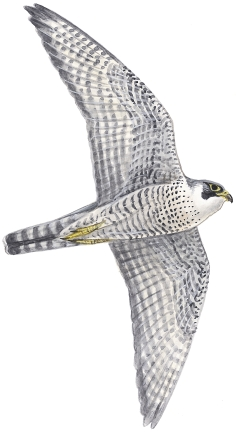
\includegraphics[height=5in]{plots/peregrine}
\vspace{4mm}

\ifthenelse{\equal{\gmxlite}{1}}
{
\fcolorbox{blue}{blue}{\textcolor{white}{\fontsize{56}{64} \selectfont Reference Manual {\em ~Lite~}}}
}
{
\fcolorbox{blue}{blue}{\textcolor{white}{\fontsize{56}{64} \selectfont ~Reference Manual~}}
} % Brace matches ifthenelse test for gmxlite
\vspace{4mm}

\textcolor{blue}{\fontsize{48}{56} \selectfont ~Version \gmxver~}


%\vspace{0.25cm}
%{\fontsize{30}{36} \selectfont \bf Version \gmxver}

\end{center}
\vfill

\ifthenelse{\equal{\gmxlite}{1}} 
{
\newpage
{\bf
This text is a shortened version of the full {\gromacs} manual, written
by David van der Spoel, Berk Hess, Erik Lindahl and others. Please
find further information on our website {\wwwpage}.}

\vspace{2cm}

\noindent \copyright\ 1991--2000: 
Department of Biophysical Chemistry, University of Groningen. 
Nijenborgh 4, 9747 AG Groningen, The Netherlands.\\
\medskip

\noindent \copyright\ 2001--{\gmxyear}:
The {\gromacs} development teams at the Royal Institute of Technology and \\
Uppsala University, Sweden.
} 
{ 
\cleardoublepage
} % Brace matches ifthenelse test for gmxlite
%reset to normal margins
\addtolength{\oddsidemargin}{5mm}

%
%       P R E F A C E
%
\renewcommand{\chaptermark}[1]{\markboth{#1}{#1}} % remember chapter title
\renewcommand{\sectionmark}[1]{\markright{\thesection\ #1}}
                                                % section number and title
\lhead[\fancyplain{}{\em\thepage}]{\fancyplain{}{\em\rightmark}}
\rhead[\fancyplain{}{\em\leftmark}]{\fancyplain{}{\em\thepage}}
\cfoot{}

\ifthenelse{\equal{\gmxlite}{1}}{}{
\begin{center}
\phantom{ }
\vspace{1cm}
{\fontsize{40}{50} \selectfont 
GROMACS\\
Reference Manual\\[1cm]
}
{\LARGE\bf Version \gmxver}\\[1cm]

{\Large 
Contributions from \\
\vspace{5mm}

\projectContributors}
\vspace{5mm}

{\LARGE \projectLeaders}
\vspace{10mm}
\end{center}

\vfill


\noindent \copyright\ 1991--2000: 
Department of Biophysical Chemistry, University of Groningen. \\
Nijenborgh 4, 9747 AG Groningen, The Netherlands.\\
\medskip

\noindent \copyright\ 2001--{\gmxyear}:
The {\gromacs} development teams at the Royal Institute of Technology and \\
Uppsala University, Sweden.

\vspace{5mm}

More information can be found on our website: {\wwwpage}.


\newpage
\pagestyle{fancyplain}

\subsection*{Preface \& Disclaimer}
This manual is not complete and has no pretention to be so due
to lack of time of the contributors -- our first priority is to improve
the software. It is worked on continuously,
which in some cases might mean the information is not entirely correct.

Comments on form and content are welcome, please send them to one of
the mailing lists (see {\wwwpage}), or open an issue
at {\redminepage}. Corrections can also be made in the GROMACS git
source repository and uploaded to {\gerritpage}.

We release an updated version of the manual whenever
we release a new version of the software, so in general 
it is a good idea to use a manual with the same major and
minor release number as your {\gromacs} installation. 

\subsection*{On-line Resources}
You can find more documentation and other material at our homepage
\wwwpage. Among other things there is an on-line reference, several
{\gromacs} mailing lists with archives and contributed
topologies/force fields.

\subsection*{Citation information}
When \normindex{citing} this document in any scientific publication
please refer to it as:
\begin{quote}
\raggedright
M.J. Abraham, D. van der Spoel, E. Lindahl, B. Hess, and the GROMACS development team,
\hspace{0.3em} {\em {\gromacs} {U}ser {M}anual version \gmxver},
\hspace{0.3em} {\wwwpage} ({\gmxyear})
\end{quote}
However, we prefer that you cite (some of) the {\gromacs}
papers~\cite{Bekker93a,Berendsen95a,Lindahl2001a,Spoel2005a,Hess2008b,Pronk2013,Pall2015,Abraham2015}
when you publish your results. Any future development depends on academic research
grants, since the package is distributed as free software!

\subsection*{{\gromacs} is {\em Free Software}}
The entire {\gromacs} package is available under the GNU Lesser
General Public License (LGPL), version 2.1. This means it's free as in free
speech, not just that you can use it without paying us money.
You can redistribute {\gromacs} and/or modify it under the terms of the LGPL
as published by the Free Software Foundation;
either version 2.1 of the License, or (at your option) any later version.
For details, check the COPYING file in the source code or consult
\href{http://www.gnu.org/licenses/old-licenses/lgpl-2.1.html}{http://www.gnu.org/licenses/old-licenses/lgpl-2.1.html}.

The {\gromacs} source code and and selected set of binary packages are
available on our homepage, \wwwpage. Have fun.
} % Brace matches ifthenelse test for gmxlite

\newpage
%       C O N T E N T S
%
\tableofcontents
%\listoffigures
%\listoftables

%
%       R E A L   M A N U A L
%
\cleardoublepage
\pagenumbering{arabic}

%
% This file is part of the GROMACS molecular simulation package.
%
% Copyright (c) 2013,2014, by the GROMACS development team, led by
% Mark Abraham, David van der Spoel, Berk Hess, and Erik Lindahl,
% and including many others, as listed in the AUTHORS file in the
% top-level source directory and at http://www.gromacs.org.
%
% GROMACS is free software; you can redistribute it and/or
% modify it under the terms of the GNU Lesser General Public License
% as published by the Free Software Foundation; either version 2.1
% of the License, or (at your option) any later version.
%
% GROMACS is distributed in the hope that it will be useful,
% but WITHOUT ANY WARRANTY; without even the implied warranty of
% MERCHANTABILITY or FITNESS FOR A PARTICULAR PURPOSE.  See the GNU
% Lesser General Public License for more details.
%
% You should have received a copy of the GNU Lesser General Public
% License along with GROMACS; if not, see
% http://www.gnu.org/licenses, or write to the Free Software Foundation,
% Inc., 51 Franklin Street, Fifth Floor, Boston, MA  02110-1301  USA.
%
% If you want to redistribute modifications to GROMACS, please
% consider that scientific software is very special. Version
% control is crucial - bugs must be traceable. We will be happy to
% consider code for inclusion in the official distribution, but
% derived work must not be called official GROMACS. Details are found
% in the README & COPYING files - if they are missing, get the
% official version at http://www.gromacs.org.
%
% To help us fund GROMACS development, we humbly ask that you cite
% the research papers on the package. Check out http://www.gromacs.org.

\chapter{Introduction}

\section{Computational Chemistry and Molecular Modeling}

\label{sec:Compchem}

{\gromacs} is an engine to perform molecular dynamics simulations and 
energy minimization. These are two of the many techniques that belong 
to the realm of \swapindex{computational}{chemistry} and 
\swapindex{molecular}{modeling}. 
{\em Computational chemistry} is just a name to indicate the use of 
computational techniques in chemistry, ranging from quantum mechanics 
of molecules to dynamics of large complex molecular aggregates. {\em 
Molecular modeling} indicates the general process of describing 
complex chemical systems in terms of a realistic atomic model, with the 
goal being to understand and predict macroscopic properties based on detailed 
knowledge on an atomic scale. Often, molecular modeling is used to 
design new materials, for which the accurate prediction of physical 
properties of realistic systems is required. 

Macroscopic physical properties can be distinguished by ($a$) {\em static 
equilibrium properties}, such as the binding constant  of an inhibitor to an 
enzyme, the average potential energy of a system, or the radial distribution  
function of a liquid, and ($b$) {\em
dynamic or non-equilibrium properties}, such as the viscosity of a 
liquid, diffusion processes in membranes, the dynamics of phase 
changes, reaction kinetics, or the dynamics of defects in crystals.  
The choice of technique depends on the question asked and on the 
feasibility of the method to yield reliable results at the present 
state of the art. Ideally, the (relativistic) time-dependent 
\swapindex{Schr{\"o}dinger}{equation} 
describes the properties of molecular systems 
with high accuracy, but anything more complex than the equilibrium 
state of a few atoms cannot be handled at this {\em ab initio} level. 
Thus, approximations are necessary; the higher the complexity of a 
system and the longer the time span of the processes of interest is, 
the more severe the required approximations are. At a certain point 
(reached very much earlier than one would wish), the {\em ab initio} 
approach must be augmented or replaced by {\em empirical} 
parameterization of the model used. Where simulations based on physical 
principles of atomic interactions still fail due to the complexity of the 
system, 
molecular modeling is based entirely on a similarity analysis of known 
structural and chemical data. The \normindex{QSAR} methods (Quantitative 
Structure-Activity Relations) and many homology-based protein structure  
predictions belong to the latter category.

Macroscopic properties are always \swapindex{ensemble}{average}s over a 
representative statistical ensemble (either equilibrium or 
non-equilibrium) of molecular systems. For molecular modeling, this has 
two important consequences:
\begin{itemize}
\item   The knowledge of a single structure, even if it is the structure 
        of the global energy minimum, is not sufficient. It is necessary to 
        generate a representative ensemble at a given temperature, in order to 
        compute macroscopic properties. But this is not enough to compute 
        thermodynamic equilibrium properties that are based on free energies, 
        such as phase equilibria, binding constants, solubilities,  relative 
        stability of molecular conformations, etc. The computation of free 
        energies and thermodynamic potentials requires special extensions of 
        molecular simulation techniques.
\item   While molecular simulations, in principle, provide atomic details 
        of the structures and motions, such details are often not relevant for 
        the macroscopic properties of interest. This opens the way to simplify 
        the description of interactions and average over irrelevant details. 
        The science of \swapindex{statistical}{mechanics} 
        provides the theoretical framework 
        for such simplifications. There is a hierarchy of methods ranging from 
        considering groups of atoms as one unit, describing motion in a 
        reduced 
        number of collective coordinates, averaging over solvent molecules 
        with 
        potentials of mean force combined with 
        \swapindex{stochastic}{dynamics}~\cite{Gunsteren90}, to {\em 
        \swapindex{mesoscopic}{dynamics}} 
        describing densities rather than atoms and fluxes 
        as response to thermodynamic gradients rather than velocities or 
        accelerations as response to forces~\cite{Fraaije93}.
\end{itemize}

For the generation of a representative equilibrium ensemble two methods 
are available: ($a$) {\em Monte Carlo simulations} and ($b$) {\em Molecular 
Dynamics simulations}. For the generation of non-equilibrium ensembles 
and for the analysis of dynamic events, only the second method is 
appropriate. While Monte Carlo simulations are more simple than MD (they 
do not require the computation of forces), they do not yield 
significantly better statistics than MD in a given amount of computer time. 
Therefore, MD is the more universal technique. If a starting 
configuration is very far from equilibrium, the forces may be 
excessively large and the MD simulation may fail. In those cases, a 
robust {\em energy minimization} is required. Another reason to perform 
an energy minimization is the removal of all kinetic energy from the 
system: if several ``snapshots'' from dynamic simulations must be compared, 
energy minimization reduces the thermal noise in the structures and  
potential energies so that they can be compared better.

\section{Molecular Dynamics Simulations}
\label{sec:MDsimulations}
MD simulations solve Newton's \swapindex{equations of}{motion} 
for a system of $N$ interacting atoms:
\beq
  m_i \frac{\partial^2 \ve{r}_i}{\partial t^2}  = \ve{F}_i, \;i=1 \ldots N.
\eeq
The forces are the negative derivatives of a potential function $V(\ve{r}_1, 
\ve{r}_2, \ldots, \ve{r}_N)$:
\beq
  \ve{F}_i = - \frac{\partial V}{\partial \ve{r}_i}
\eeq
The equations are solved simultaneously in small time steps. The
system is followed for some time, taking care that the temperature and
pressure remain at the required values, and the coordinates are
written to an output file at regular intervals. The coordinates as a
function of time represent a {\em trajectory} of the system. After
initial changes, the system will usually reach an {\em equilibrium
state}. By averaging over an equilibrium trajectory, many macroscopic
properties can be extracted from the output file.

It is useful at this point to consider the \normindex{limitations} of MD
simulations. The user should be aware of those limitations and always
perform checks on known experimental properties to assess the accuracy
of the simulation. We list the approximations below.

\begin{description}
\item[{\bf The simulations are classical}]\mbox{}\\
Using Newton's equation of motion automatically implies the use of
{\em classical mechanics} to describe the motion of atoms. This is
all right for most atoms at normal temperatures, but there are
exceptions. Hydrogen atoms are quite light and the motion of protons
is sometimes of essential quantum mechanical character. For example, a
proton may {\em tunnel} through a potential barrier in the course of a
transfer over a hydrogen bond. Such processes cannot be properly
treated by classical dynamics! Helium liquid at low temperature is
another example where classical mechanics breaks down. While helium
may not deeply concern us, the high frequency vibrations of covalent
bonds should make us worry! The statistical mechanics of a classical
harmonic oscillator differs appreciably from that of a real quantum
oscillator when the resonance frequency $\nu$ approximates or exceeds
$k_BT/h$. Now at room temperature the wavenumber $\sigma = 1/\lambda =
\nu/c$ at which $h
\nu = k_BT$ is approximately 200 cm$^{-1}$. Thus, all frequencies
higher than, say, 100 cm$^{-1}$ may misbehave in
classical simulations. This means that practically all bond and
bond-angle vibrations are suspect, and even hydrogen-bonded motions as
translational or librational H-bond vibrations are beyond the
classical limit (see \tabref{vibrations}). What can we do?

\begin{table}
\begin{center} 
\begin{tabular}{|l|l|r@{--}rl|}
\dline
                & \mcc{1}{type of}   & \mcc{3}{wavenumber}  \\
type of bond    & \mcc{1}{vibration} & \mcc{3}{(cm$^{-1}$)} \\
\hline
C-H, O-H, N-H   & stretch       & 3000  & 3500  & \\
C=C, C=O        & stretch       & 1700  & 2000  & \\
HOH             & bending       & \mcl{2}{1600} & \\
C-C             & stretch       & 1400  & 1600  & \\
H$_2$CX         & sciss, rock   & 1000  & 1500  & \\ 
CCC             & bending       &  800  & 1000  & \\
O-H$\cdots$O    & libration     &  400  & 700   & \\
O-H$\cdots$O    & stretch       &   50  & 200   & \\
\dline
\end{tabular} 
\end{center} 
\caption[Typical vibrational frequencies.]{Typical vibrational
frequencies (wavenumbers) in molecules and hydrogen-bonded
liquids. Compare $kT/h = 200$ cm$^{-1}$ at 300~K.}
\label{tab:vibrations}
\end{table}

Well, apart from real quantum-dynamical simulations, we can do one
of two things: \\ (a) If we perform MD simulations using harmonic
oscillators for bonds, we should make corrections to the total
internal energy $U = E_{kin} + E_{pot}$ and specific heat $C_V$ (and
to entropy $S$ and free energy $A$ or $G$ if those are
calculated). The corrections to the energy and specific heat of a
one-dimensional oscillator with frequency $\nu$
are:~\cite{McQuarrie76}
\beq
 U^{QM} = U^{cl} +kT \left( \half x - 1 + \frac{x}{e^x-1} \right)
\eeq
\beq
 C_V^{QM} = C_V^{cl} + k \left( \frac{x^2e^x}{(e^x-1)^2} - 1 \right), 
\eeq
where $x=h\nu /kT$. The classical oscillator absorbs too much energy
($kT$), while the high-frequency quantum oscillator is in its ground
state at the zero-point energy level of $\frac{1}{2} h\nu$. \\ (b) We
can treat the bonds (and bond angles) as {\em \normindex{constraint}s}
in the equations of motion. The rationale behind this is that a quantum
oscillator in its ground state resembles a constrained bond more
closely than a classical oscillator. A good practical reason for this
choice is that the algorithm can use larger time steps when the
highest frequencies are removed. In practice the time step can be made
four times as large when bonds are constrained than when they are
oscillators~\cite{Gunsteren77}. {\gromacs} has this option for the
bonds and bond angles.  The flexibility of the latter is
rather essential to allow for the realistic motion and coverage of
configurational space~\cite{Gunsteren82}.

\item[{\bf Electrons are in the ground state}]\mbox{}\\
In MD we use a {\em conservative} force field that is a
function of the positions of atoms only.  This means that the
electronic motions are not considered: the electrons are supposed to
adjust their dynamics instantly when the atomic positions change
(the {\em \normindex{Born-Oppenheimer}} approximation), and remain in
their ground state. This is really all right, almost always. But of
course, electron transfer processes and electronically excited states
can not be treated. Neither can chemical reactions be treated
properly, but there are other reasons to shy away from reactions for
the time being.

\item[{\bf Force fields are approximate}]\mbox{}\\
Force fields \index{force field} provide the forces.
They are not really a part of the
simulation method and their parameters can be modified by the user as the
need arises or knowledge improves. But the form of the forces that can
be used in a particular program is subject to limitations. The force
field that is incorporated in {\gromacs} is described in Chapter 4. In
the present version the force field is pair-additive (apart from
long-range Coulomb forces), it cannot incorporate
polarizabilities, and it does not contain fine-tuning of bonded
interactions. This urges the inclusion of some limitations in this
list below.  For the rest it is quite useful and fairly reliable for
biologically-relevant macromolecules in aqueous solution!

\item[{\bf The force field is pair-additive}]\mbox{}\\
This means that all {\em non-bonded} forces result from the sum of
non-bonded pair interactions. Non pair-additive interactions, the most
important example of which is interaction through atomic
polarizability, are represented by {\em effective pair
potentials}. Only average non pair-additive contributions are
incorporated. This also means that the pair interactions are not pure,
{\ie}, they are not valid for isolated pairs or for situations
that differ appreciably from the test systems on which the models were
parameterized. In fact, the effective pair potentials are not that bad
in practice. But the omission of polarizability also means that
electrons in atoms do not provide a dielectric constant as they
should. For example, real liquid alkanes have a dielectric constant of
slightly more than 2, which reduce the long-range electrostatic
interaction between (partial) charges. Thus, the simulations will
exaggerate the long-range Coulomb terms. Luckily, the next item
compensates this effect a bit.

\item[{\bf Long-range interactions are cut off}]\mbox{}\\
In this version, {\gromacs} always uses a \normindex{cut-off} radius for the
Lennard-Jones interactions and sometimes for the Coulomb interactions
as well. The ``minimum-image convention'' used by {\gromacs} requires that only one image of each
particle in the periodic boundary conditions is considered for a pair
interaction, so the cut-off radius cannot exceed half the box size. That
is still pretty big for large systems, and trouble is only expected
for systems containing charged particles. But then truly bad things can
happen, like accumulation of charges at the cut-off boundary or very
wrong energies! For such systems, you should consider using one of the
implemented long-range electrostatic algorithms, such as 
particle-mesh Ewald~\cite{Darden93,Essmann95}.

\item[{\bf Boundary conditions are unnatural}]\mbox{}\\
Since system size is small (even 10,000 particles is small), a cluster
of particles will have a lot of unwanted boundary with its environment
(vacuum). We must avoid this condition if we wish to simulate a bulk system.
As such, we use periodic boundary conditions to avoid real phase
boundaries. Since liquids are not crystals, something unnatural
remains. This item is mentioned last because it is the
least of the evils. For large systems, the errors are small, but for
small systems with a lot of internal spatial correlation, the periodic
boundaries may enhance internal correlation. In that case, beware of, and
test, the influence of system size. This is especially important when
using lattice sums for long-range electrostatics, since these are known
to sometimes introduce extra ordering.
\end{description}

\section{Energy Minimization and Search Methods}

As mentioned in \secref{Compchem}, in many cases energy minimization
is required. {\gromacs} provides a number of methods for local energy
minimization, as detailed in \secref{EM}.

The potential energy function of a (macro)molecular system is a very
complex landscape (or {\em hypersurface}) in a large number of
dimensions. It has one deepest point, the {\em global minimum} and a
very large number of {\em local minima}, where all derivatives of the
potential energy function with respect to the coordinates are zero and
all second derivatives are non-negative. The matrix of second
derivatives, which is called the {\em Hessian matrix}, has non-negative
eigenvalues; only the collective coordinates that correspond to
translation and rotation (for an isolated molecule) have zero
eigenvalues. In between the local minima there are {\em saddle
points}, where the Hessian matrix has only one negative
eigenvalue. These points are the mountain passes through which the
system can migrate from one local minimum to another.

Knowledge of all local minima, including the global one, and of all
saddle points would enable us to describe the relevant structures and
conformations and their free energies, as well as the dynamics of
structural transitions. Unfortunately, the dimensionality of the
configurational space and the number of local minima is so high that
it is impossible to sample the space at a sufficient number of points
to obtain a complete survey. In particular, no minimization method
exists that guarantees the determination of the global minimum in any
practical amount of time. Impractical methods exist, some much faster
than others~\cite{Geman84}.  However, given a starting configuration,
it is possible to find the {\em nearest local minimum}. ``Nearest'' in
this context does not always imply ``nearest'' in a geometrical sense
({\ie}, the least sum of square coordinate differences), but means the
minimum that can be reached by systematically moving down the steepest
local gradient. Finding this nearest local minimum is all that
{\gromacs} can do for you, sorry! If you want to find other minima and
hope to discover the global minimum in the process, the best advice is
to experiment with temperature-coupled MD: run your system at a high
temperature for a while and then quench it slowly down to the required
temperature; do this repeatedly!  If something as a melting or glass
transition temperature exists, it is wise to stay for some time
slightly below that temperature and cool down slowly according to some
clever scheme, a process called {\em simulated annealing}. Since no
physical truth is required, you can use your imagination to speed up this
process. One trick that often works is to make hydrogen atoms heavier
(mass 10 or so): although that will slow down the otherwise very rapid
motions of hydrogen atoms, it will hardly influence the slower motions
in the system, while enabling you to increase the time step by a factor
of 3 or 4. You can also modify the potential energy function during
the search procedure, {\eg} by removing barriers (remove dihedral
angle functions or replace repulsive potentials by {\em soft-core}
potentials~\cite{Nilges88}), but always take care to restore the
correct functions slowly. The best search method that allows rather
drastic structural changes is to allow excursions into
four-dimensional space~\cite{Schaik93}, but this requires some extra
programming beyond the standard capabilities of {\gromacs}.

Three possible energy minimization methods are:
\begin{itemize}
\item   Those that require only function evaluations. Examples are the 
        simplex method and its variants. A step is made on the basis of the 
        results of previous evaluations. If derivative information is 
        available, such methods are inferior to those that use 
        this information.
\item   Those that use derivative information. Since the partial 
        derivatives of the potential energy with respect to all 
        coordinates are known in MD programs (these are equal to minus 
        the forces) this class of methods is very suitable as modification 
        of MD programs.
\item   Those that use second derivative information as well. These methods 
        are superior in their convergence properties near the minimum: a 
        quadratic potential function is minimized in one step! The problem 
        is that for $N$ particles a $3N\times 3N$ matrix must be computed, 
        stored, and inverted. Apart from the extra programming to obtain 
        second derivatives, for most systems of interest this is beyond the 
        available capacity. There are intermediate methods that build up the 
        Hessian matrix on the fly, but they also suffer from excessive 
        storage requirements. So {\gromacs} will shy away from this class 
        of methods.
\end{itemize}


The {\em steepest descent} method, available in {\gromacs}, is of the
second class. It simply takes a step in the direction of the negative
gradient (hence in the direction of the force), without any
consideration of the history built up in previous steps. The step size
is adjusted such that the search is fast, but the motion is always
downhill. This is a simple and sturdy, but somewhat stupid, method:
its convergence can be quite slow, especially in the vicinity of the
local minimum! The faster-converging {\em conjugate gradient method}
(see {\eg} \cite{Zimmerman91}) uses gradient information from previous
steps. In general, steepest descents will bring you close to the
nearest local minimum very quickly, while conjugate gradients brings
you {\em very} close to the local minimum, but performs worse far away
from the minimum. {\gromacs} also supports the L-BFGS minimizer, which
is mostly comparable to {\em conjugate gradient method}, but in some 
cases converges faster.

% LocalWords:  Schr dinger initio parameterization QSAR equilibria solubilities
% LocalWords:  mesoscopic BT wavenumber rl HOH CX sciss CCC libration kT minima
% LocalWords:  wavenumbers polarizabilities polarizability parameterized BFGS
% LocalWords:  alkanes Compchem librational configurational Ewald
% LocalWords:  hypersurface

%
% This file is part of the GROMACS molecular simulation package.
%
% Copyright (c) 2013,2014,2015,2016, by the GROMACS development team, led by
% Mark Abraham, David van der Spoel, Berk Hess, and Erik Lindahl,
% and including many others, as listed in the AUTHORS file in the
% top-level source directory and at http://www.gromacs.org.
%
% GROMACS is free software; you can redistribute it and/or
% modify it under the terms of the GNU Lesser General Public License
% as published by the Free Software Foundation; either version 2.1
% of the License, or (at your option) any later version.
%
% GROMACS is distributed in the hope that it will be useful,
% but WITHOUT ANY WARRANTY; without even the implied warranty of
% MERCHANTABILITY or FITNESS FOR A PARTICULAR PURPOSE.  See the GNU
% Lesser General Public License for more details.
%
% You should have received a copy of the GNU Lesser General Public
% License along with GROMACS; if not, see
% http://www.gnu.org/licenses, or write to the Free Software Foundation,
% Inc., 51 Franklin Street, Fifth Floor, Boston, MA  02110-1301  USA.
%
% If you want to redistribute modifications to GROMACS, please
% consider that scientific software is very special. Version
% control is crucial - bugs must be traceable. We will be happy to
% consider code for inclusion in the official distribution, but
% derived work must not be called official GROMACS. Details are found
% in the README & COPYING files - if they are missing, get the
% official version at http://www.gromacs.org.
%
% To help us fund GROMACS development, we humbly ask that you cite
% the research papers on the package. Check out http://www.gromacs.org.

\chapter{Definitions and Units}
\label{ch:defunits}
\section{Notation}
The following conventions for mathematical typesetting 
are used throughout this document:

\centerline{
\begin{tabular}{l|l|c}
Item		&	Notation	& Example	\\
\hline	
Vector		&	Bold italic	& $\rvi$	\\
Vector Length	&	Italic		& $r_i$		\\
\end{tabular}
}

We define the {\em lowercase} subscripts 
$i$, $j$, $k$ and $l$ to denote particles:
$\rvi$ is the {\em position vector} of particle $i$, and using this 
notation:
\bea
\rvij	=	\rvj-\rvi	\\
\rij	=	| \rvij |
\eea
The force on particle $i$ is denoted by $\ve{F}_i$ and 
\beq
\ve{F}_{ij} = \mbox{force on $i$ exerted by $j$}
\eeq
Please note that we changed notation as of version 2.0 to $\rvij=\rvj-\rvi$ since this
is the notation commonly used. If you encounter an error, let us know.

\section{\normindex{MD units}\index{units}}
{\gromacs} uses a consistent set of units that produce values in the
vicinity of unity for most relevant molecular quantities. Let us call
them {\em MD units}. The basic units in this system are nm, ps, K,
electron charge (e) and atomic mass unit (u), see
\tabref{basicunits}. The values used in {\gromacs}  are taken from the
CODATA Internationally recommended 2010 values of 
fundamental physical constants (see \verb+http://nist.gov+).
\begin{table}
\centerline{
\begin{tabular}{|l|c|l|}
\dline
Quantity	& Symbol&  Unit						\\
\hline			
length		&  r	&  nm $= 10^{-9}$ m				\\
mass		&  m	&  u (unified atomic mass unit)	$=$ 
				$1.660\,538\,921 \times 10^{-27}$ kg	\\
time		&  t	&  ps $= 10^{-12}$ s				\\
charge		&  q	&  {\it e} $=$ elementary charge $=
				1.602\,176\,565(\times 10^{-19}$ C	\\
temperature	&  T	&  K  						\\
\dline
\end{tabular}
}
\caption[Basic units used in {\gromacs}.]{Basic units used in
{\gromacs}.}
\label{tab:basicunits}
\end{table}

Consistent with these units are a set of derived units, given in
\tabref{derivedunits}.
\begin{table}
\centerline{
\begin{tabular}{|l|c|l|}
\dline
Quantity	& Symbol   & Unit				\\
\hline
energy		& $E,V$	   & kJ~mol$^{-1}$			\\
Force		& $\ve{F}$ & kJ~mol$^{-1}$~nm$^{-1}$		\\
pressure	& $p$	   & bar                               \\
velocity	& $v$	   & nm~ps$^{-1} = 1000$ m s$^{-1}$		\\
dipole moment   & $\mu$	   & \emph{e}~nm                		\\ 
electric potential& $\Phi$ & kJ~mol$^{-1}$~\emph{e}$^{-1} = 
				0.010\,364\,269\,19$ Volt   	\\
electric field	& $E$	   & kJ~mol$^{-1}$~nm$^{-1}$~\emph{e}$^{-1} =
 				1.036\,426\,919 \times 10^7$~V m$^{-1}$	\\
\dline
\end{tabular}
}
\caption{Derived units. Note that an additional conversion factor of 10$^{28}$ a.m.u ($\approx$16.6)
is applied to get bar instead of internal MD units in the energy and
log files.}
\label{tab:derivedunits}
\end{table}

The {\bf electric conversion factor} $f=\frac{1}{4 \pi
\varepsilon_o}=\electricConvFactorValue$ kJ~mol$^{-1}$~nm~e$^{-2}$. It relates
the mechanical quantities to the electrical quantities as in
\beq
 V = f \frac{q^2}{r} \mbox{\ \ or\ \ } F = f \frac{q^2}{r^2}
\eeq

Electric potentials $\Phi$ and electric fields $\ve{E}$ are
intermediate quantities in the calculation of energies and
forces. They do not occur inside {\gromacs}. If they are used in
evaluations, there is a choice of equations and related units. We
strongly recommend following the usual practice of including the factor
$f$ in expressions that evaluate $\Phi$ and $\ve{E}$:
\bea
\Phi(\ve{r}) = f \sum_j \frac{q_j}{|\ve{r}-\ve{r}_j|} 	\\
\ve{E}(\ve{r}) = f \sum_j q_j \frac{(\ve{r}-\ve{r}_j)}{|\ve{r}-\ve{r}_j|^3}
\eea
With these definitions, $q\Phi$ is an energy and $q\ve{E}$ is a
force. The units are those given in \tabref{derivedunits}:
about 10 mV for potential. Thus, the potential of an electronic charge
at a distance of 1 nm equals $f \approx 140$ units $\approx
1.4$~V. (exact value: $1.439\,964\,5$ V)

{\bf Note} that these units are mutually consistent; changing any of the
units is likely to produce inconsistencies and is therefore {\em
strongly discouraged\/}! In particular: if \AA \ are used instead of
nm, the unit of time changes to 0.1 ps. If kcal mol$^{-1}$ (= 4.184
kJ mol$^{-1}$) is used instead of kJ mol$^{-1}$ for energy, the unit of time becomes
0.488882 ps and the unit of temperature changes to 4.184 K. But in
both cases all electrical energies go wrong, because they will still
be computed in kJ mol$^{-1}$, expecting nm as the unit of length. Although
careful rescaling of charges may still yield consistency, it is clear
that such confusions must be rigidly avoided.
  
In terms of the MD units, the usual physical constants take on
different values (see \tabref{consts}). All quantities are per mol rather than per
molecule. There is no distinction between Boltzmann's constant $k$ and
the gas constant $R$: their value is
$0.008\,314\,462\,1$~kJ~mol$^{-1}$~K$^{-1}$.
\begin{table}
\centerline{
\begin{tabular}{|c|l|l|}
\dline
Symbol	& Name			& Value					\\
\hline
$N_{AV}$& Avogadro's number 	& $6.022\,141\,29\times 10^{23}$  mol$^{-1}$	\\
$R$   	& gas constant 	& $8.314\,462\,1\times 10^{-3}$~kJ~mol$^{-1}$~K$^{-1}$	\\
$k_B$  	& Boltzmann's constant  & \emph{idem}	\\
$h$	& Planck's constant	& $0.399\,031\,271$~kJ~mol$^{-1}$~ps \\
$\hbar$	& Dirac's constant	& $0.063\,507\,799\,3$~kJ~mol$^{-1}$~ps \\
$c$	& velocity of light	& $299\,792.458$~nm~ps$^{-1}$ \\
\dline
\end{tabular}
}
\caption{Some Physical Constants}
\label{tab:consts}
\end{table}

\section{Reduced units\index{reduced units}}
When simulating Lennard-Jones (LJ) systems, it might be advantageous to
use reduced units ({\ie}, setting
$\epsilon_{ii}=\sigma_{ii}=m_i=k_B=1$ for one type of atoms). This is
possible. When specifying the input in reduced units, the output will
also be in reduced units. The one exception is the {\em
temperature}, which is expressed in $0.008\,314\,462\,1$ reduced
units. This is a consequence of using Boltzmann's constant in the
evaluation of temperature in the code. Thus not $T$, but $k_BT$, is the
reduced temperature. A {\gromacs} temperature $T=1$ means a reduced
temperature of $0.008\ldots$ units; if a reduced temperature of 1 is
required, the {\gromacs} temperature should be $120.272\,36$.

In \tabref{reduced} quantities are given for LJ potentials:
\beq
V_{LJ} = 4\epsilon \left[ \left(\frac{\sigma}{r}\right)^{12} - \left(\frac{\sigma}{r}\right)^{6} \right]
\eeq

\begin{table}
\centerline{
\begin{tabular}{|l|c|l|}
\dline
Quantity	& Symbol	& Relation to SI			\\
\hline
Length		& r$^*$  	& r $\sigma^{-1}$			\\
Mass		& m$^*$  	& m M$^{-1}$				\\
Time		& t$^*$  	& t $\sigma^{-1}$ $\sqrt{\epsilon/M}$ \\
Temperature  	& T$^*$  	& k$_B$T $\epsilon^{-1}$ 		\\
Energy		& E$^*$  	& E $\epsilon^{-1}$           	\\
Force		& F$^*$  	& F $\sigma~\epsilon^{-1}$		\\
Pressure	& P$^*$  	& P $\sigma ^3 \epsilon^{-1}$		\\
Velocity	& v$^*$  	& v $\sqrt{M/\epsilon}$		\\
Density		& $\rho^*$  	& N $\sigma ^3~V^{-1}$		\\
\dline
\end{tabular}
}
\caption{Reduced Lennard-Jones quantities}
\label{tab:reduced}
\end{table}


\section{Mixed or Double precision}
{\gromacs} can be compiled in either mixed\index{mixed
precision|see{precision, mixed}}\index{precision, mixed} or
\pawsindex{double}{precision}. Documentation of previous {\gromacs}
versions referred to ``single precision'', but the implementation
has made selective use of double precision for many years.
Using single precision
for all variables would lead to a significant reduction in accuracy.
Although in ``mixed precision'' all state vectors, i.e. particle coordinates,
velocities and forces, are stored in single precision, critical variables
are double precision. A typical example of the latter is the virial,
which is a sum over all forces in the system, which have varying signs.
In addition, in many parts of the code we managed to avoid double precision
for arithmetic, by paying attention to summation order or reorganization
of mathematical expressions. The default configuration uses mixed precision,
but it is easy to turn on double precision by adding the option
{\tt -DGMX_DOUBLE=on} to {\tt cmake}. Double precision
will be 20 to 100\% slower than mixed precision depending on the
architecture you are running on. Double precision will use somewhat
more memory and run input, energy and full-precision trajectory files
will be almost twice as large.

The energies in mixed precision are accurate up to the last decimal,
the last one or two decimals of the forces are non-significant.
The virial is less accurate than the forces, since the virial is only one
order of magnitude larger than the size of each element in the sum over
all atoms (\secref{virial}).
In most cases this is not really a problem, since the fluctuations in the
virial can be two orders of magnitude larger than the average.
Using cut-offs for the Coulomb interactions cause large errors
in the energies, forces, and virial.
Even when using a reaction-field or lattice sum method, the errors
are larger than, or comparable to, the errors due to the partial use of
single precision.
Since MD is chaotic, trajectories with very similar starting conditions will
diverge rapidly, the divergence is faster in mixed precision than in double
precision.

For most simulations, mixed precision is accurate enough.
In some cases double precision is required to get reasonable results:
\begin{itemize}
\item normal mode analysis,
for the conjugate gradient or l-bfgs minimization and the calculation and
diagonalization of the Hessian
\item long-term energy conservation, especially for large systems
\end{itemize}


% LocalWords:  ij basicunits derivedunits kJ mol mV kcal consts LJ BT
% LocalWords:  nm ps

%
% This file is part of the GROMACS molecular simulation package.
%
% Copyright (c) 2013,2014,2015,2016,2017, by the GROMACS development team, led by
% Mark Abraham, David van der Spoel, Berk Hess, and Erik Lindahl,
% and including many others, as listed in the AUTHORS file in the
% top-level source directory and at http://www.gromacs.org.
%
% GROMACS is free software; you can redistribute it and/or
% modify it under the terms of the GNU Lesser General Public License
% as published by the Free Software Foundation; either version 2.1
% of the License, or (at your option) any later version.
%
% GROMACS is distributed in the hope that it will be useful,
% but WITHOUT ANY WARRANTY; without even the implied warranty of
% MERCHANTABILITY or FITNESS FOR A PARTICULAR PURPOSE.  See the GNU
% Lesser General Public License for more details.
%
% You should have received a copy of the GNU Lesser General Public
% License along with GROMACS; if not, see
% http://www.gnu.org/licenses, or write to the Free Software Foundation,
% Inc., 51 Franklin Street, Fifth Floor, Boston, MA  02110-1301  USA.
%
% If you want to redistribute modifications to GROMACS, please
% consider that scientific software is very special. Version
% control is crucial - bugs must be traceable. We will be happy to
% consider code for inclusion in the official distribution, but
% derived work must not be called official GROMACS. Details are found
% in the README & COPYING files - if they are missing, get the
% official version at http://www.gromacs.org.
%
% To help us fund GROMACS development, we humbly ask that you cite
% the research papers on the package. Check out http://www.gromacs.org.

\newcommand{\nproc}{\mbox{$M$}}
\newcommand{\natom}{\mbox{$N$}}
\newcommand{\nx}{\mbox{$n_x$}}
\newcommand{\ny}{\mbox{$n_y$}}
\newcommand{\nz}{\mbox{$n_z$}}
\newcommand{\nsgrid}{NS grid}
\newcommand{\fftgrid}{FFT grid}
\newcommand{\dgrid}{\mbox{$\delta_{grid}$}}
\newcommand{\bfv}[1]{{\mbox{\boldmath{$#1$}}}}
% non-italicized boldface for math (e.g. matrices)                              
\newcommand{\bfm}[1]{{\bf #1}}
\newcommand{\dt}{\Delta t}
\newcommand{\rv}{\bfv{r}}
\newcommand{\vv}{\bfv{v}}
\newcommand{\F}{\bfv{F}}
\newcommand{\pb}{\bfv{p}}
\newcommand{\veps}{v_{\epsilon}}
\newcommand{\peps}{p_{\epsilon}}
\newcommand{\sinhx}[1]{\frac{\sinh{\left( #1\right)}}{#1}}
\chapter{Algorithms}
\label{ch:algorithms}
\section{Introduction}
In this chapter we first give describe some general concepts used in
{\gromacs}:  {\em periodic boundary conditions} (\secref{pbc})
and the {\em group concept} (\secref{groupconcept}). The MD algorithm is
described in \secref{MD}: first a global form of the algorithm is
given, which is refined in subsequent subsections. The (simple) EM
(Energy Minimization) algorithm is described in \secref{EM}. Some
other algorithms for special purpose dynamics are described after
this.  

%\ifthenelse{\equal{\gmxlite}{1}}{}{
%In the final \secref{par} of this chapter a few principles are
%given on which parallelization of {\gromacs} is based. The
%parallelization is hardly visible for the user and is therefore not
%treated in detail.
%} % Brace matches ifthenelse test for gmxlite

A few issues are of general interest. In all cases the {\em system}
must be defined, consisting of molecules. Molecules again consist of
particles  with defined interaction functions. The detailed
description of the {\em topology} of the molecules and of the {\em force
field} and the calculation of forces is given in
\chref{ff}. In the present chapter we describe
other aspects of the algorithm, such as pair list generation, update of
velocities  and positions, coupling to external temperature and
pressure,  conservation of constraints. 
\ifthenelse{\equal{\gmxlite}{1}}{}{
The {\em analysis} of the data generated by an MD simulation is treated in \chref{analysis}.
} % Brace matches ifthenelse test for gmxlite

\section{Periodic boundary conditions\index{periodic boundary conditions}}
\label{sec:pbc}
\begin{figure}
\centerline{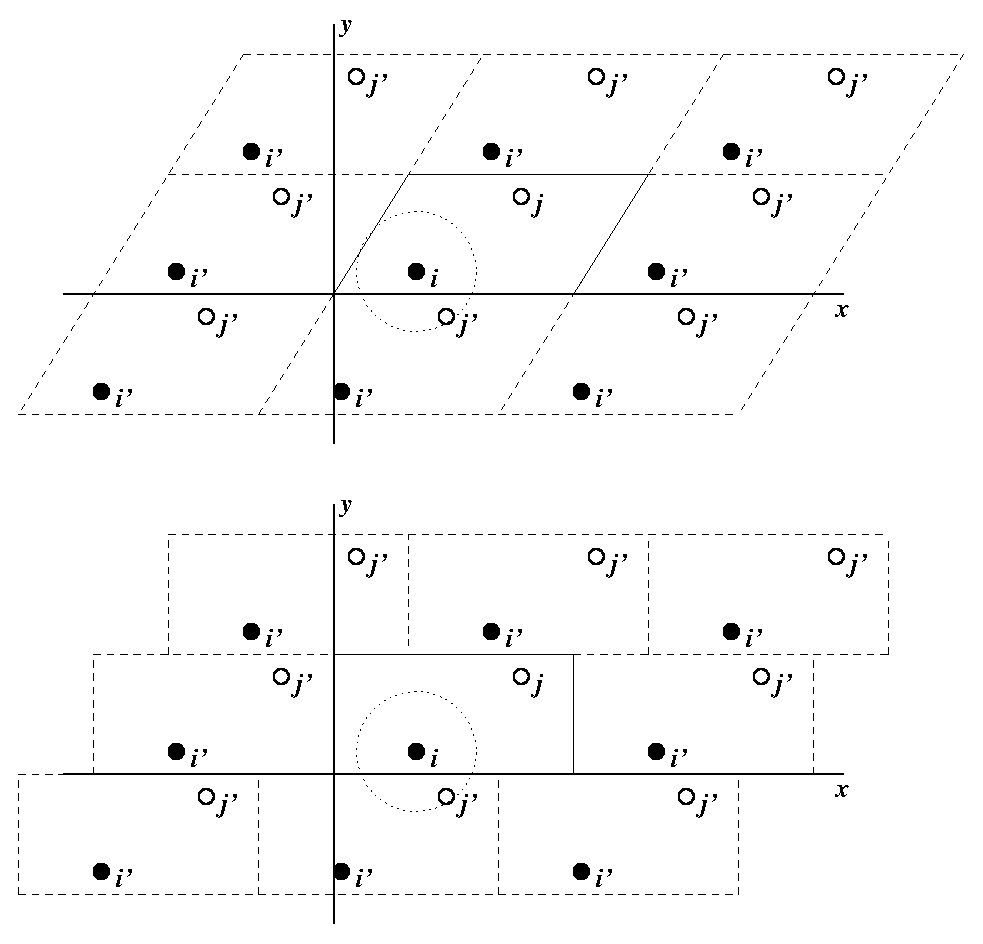
\includegraphics[width=9cm]{plots/pbctric}}
\caption {Periodic boundary conditions in two dimensions.}
\label{fig:pbc}
\end{figure}
The classical way to minimize edge effects in a finite system is to
apply {\em periodic boundary conditions}. The atoms of the system to
be simulated are put into a space-filling box, which is surrounded by
translated copies of itself (\figref{pbc}).  Thus there are no
boundaries of the system; the artifact caused by unwanted boundaries
in an isolated cluster is now replaced by the artifact of periodic
conditions. If the system is crystalline, such boundary conditions are
desired (although motions are naturally restricted to periodic motions
with wavelengths fitting into the box). If one wishes to simulate
non-periodic systems, such as liquids or solutions, the periodicity by
itself causes errors. The errors can be evaluated by comparing various
system sizes; they are expected to be less severe than the errors
resulting from an unnatural boundary with vacuum.

There are several possible shapes for space-filling unit cells. Some,
like the {\em \normindex{rhombic dodecahedron}} and the
{\em \normindex{truncated octahedron}}~\cite{Adams79} are closer to being a sphere
than a cube is, and are therefore better suited to the 
study of an approximately spherical macromolecule in solution, since
fewer solvent molecules are required to fill the box given a minimum
distance between macromolecular images. At the same time, rhombic 
dodecahedra and truncated octahedra are special cases of {\em triclinic} 
unit cells\index{triclinic unit cell}; the most general space-filling unit cells
that comprise all possible space-filling shapes~\cite{Bekker95}.
For this reason, {\gromacs} is based on the triclinic unit cell.
  
{\gromacs} uses periodic boundary conditions, combined with the {\em
\normindex{minimum image convention}}: only one -- the nearest -- image of each
particle is considered for short-range non-bonded interaction terms.
For long-range electrostatic interactions this is not always accurate
enough, and {\gromacs} therefore also incorporates lattice sum methods
such as Ewald Sum, PME and PPPM.

{\gromacs} supports triclinic boxes of any shape.
The simulation box (unit cell) is defined by the 3 box vectors 
${\bf a}$,${\bf b}$ and ${\bf c}$.
The box vectors must satisfy the following conditions:
\beq
\label{eqn:box_rot}
a_y = a_z = b_z = 0
\eeq
\beq
\label{eqn:box_shift1}
a_x>0,~~~~b_y>0,~~~~c_z>0
\eeq
\beq
\label{eqn:box_shift2}
|b_x| \leq \frac{1}{2} \, a_x,~~~~
|c_x| \leq \frac{1}{2} \, a_x,~~~~
|c_y| \leq \frac{1}{2} \, b_y
\eeq
Equations \ref{eqn:box_rot} can always be satisfied by rotating the box.
Inequalities (\ref{eqn:box_shift1}) and (\ref{eqn:box_shift2}) can always be
satisfied by adding and subtracting box vectors.

Even when simulating using a triclinic box, {\gromacs} always keeps the
particles in a brick-shaped volume for efficiency,
as illustrated in \figref{pbc} for a 2-dimensional system.
Therefore, from the output trajectory it might seem that the simulation was
done in a rectangular box. The program {\tt trjconv} can be used to convert 
the trajectory to a different unit-cell representation.

It is also possible to simulate without periodic boundary conditions,
but it is usually more efficient to simulate an isolated cluster of molecules
in a large periodic box, since fast grid searching can only be used 
in a periodic system.

\begin{figure}
\centerline{
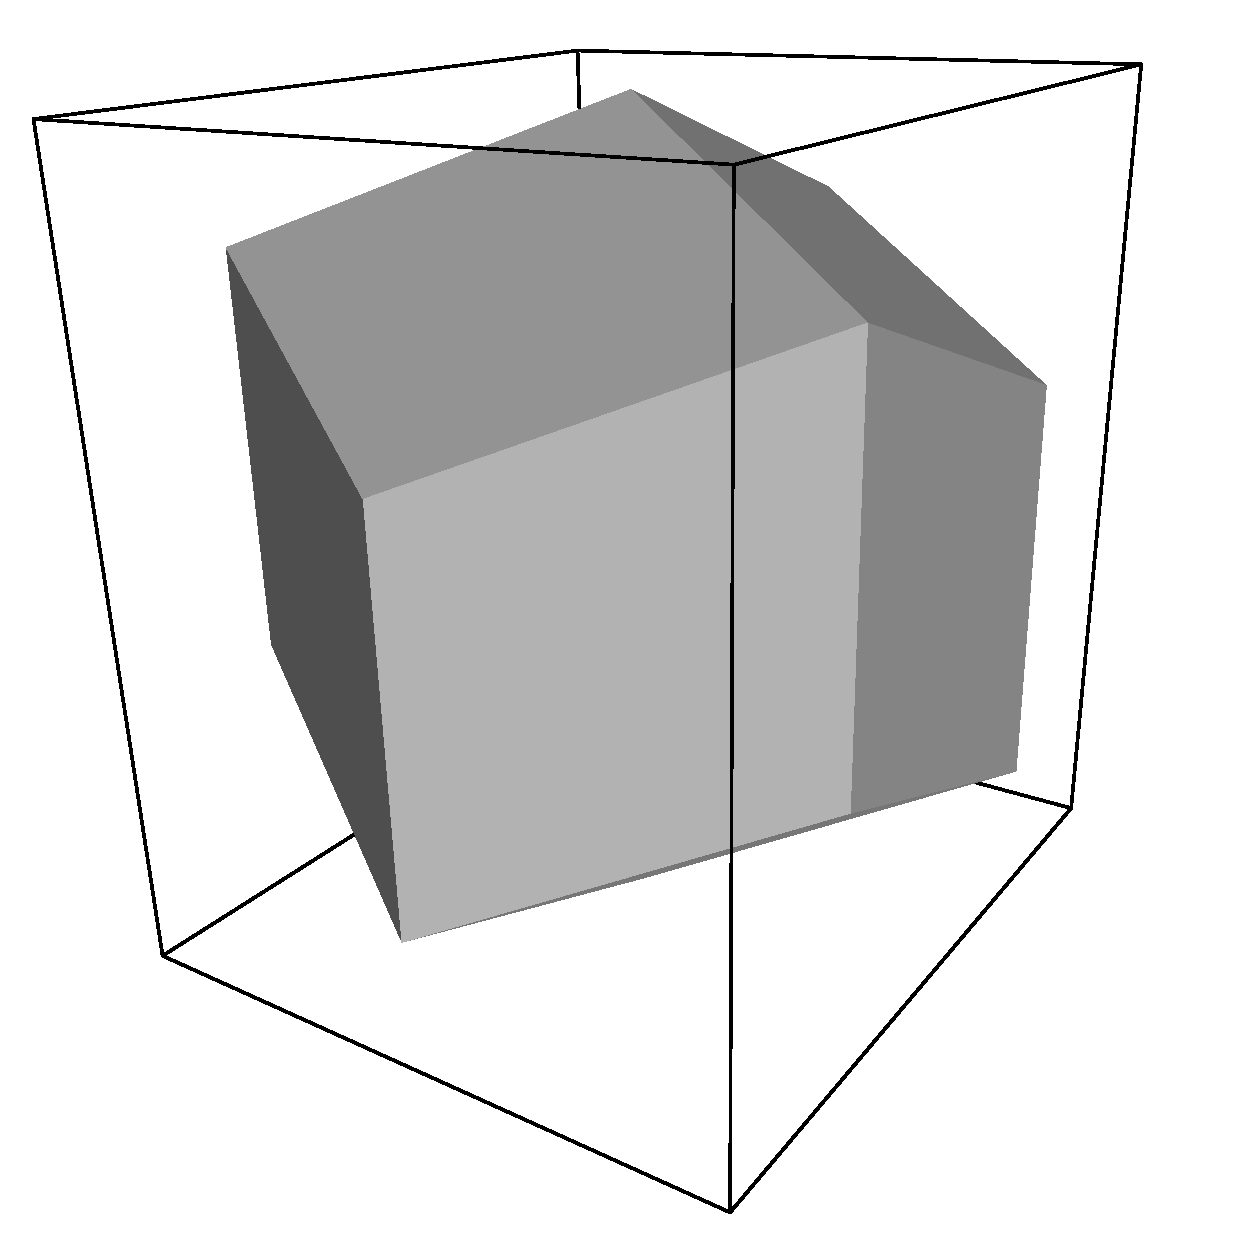
\includegraphics[width=5cm]{plots/rhododec}
~~~~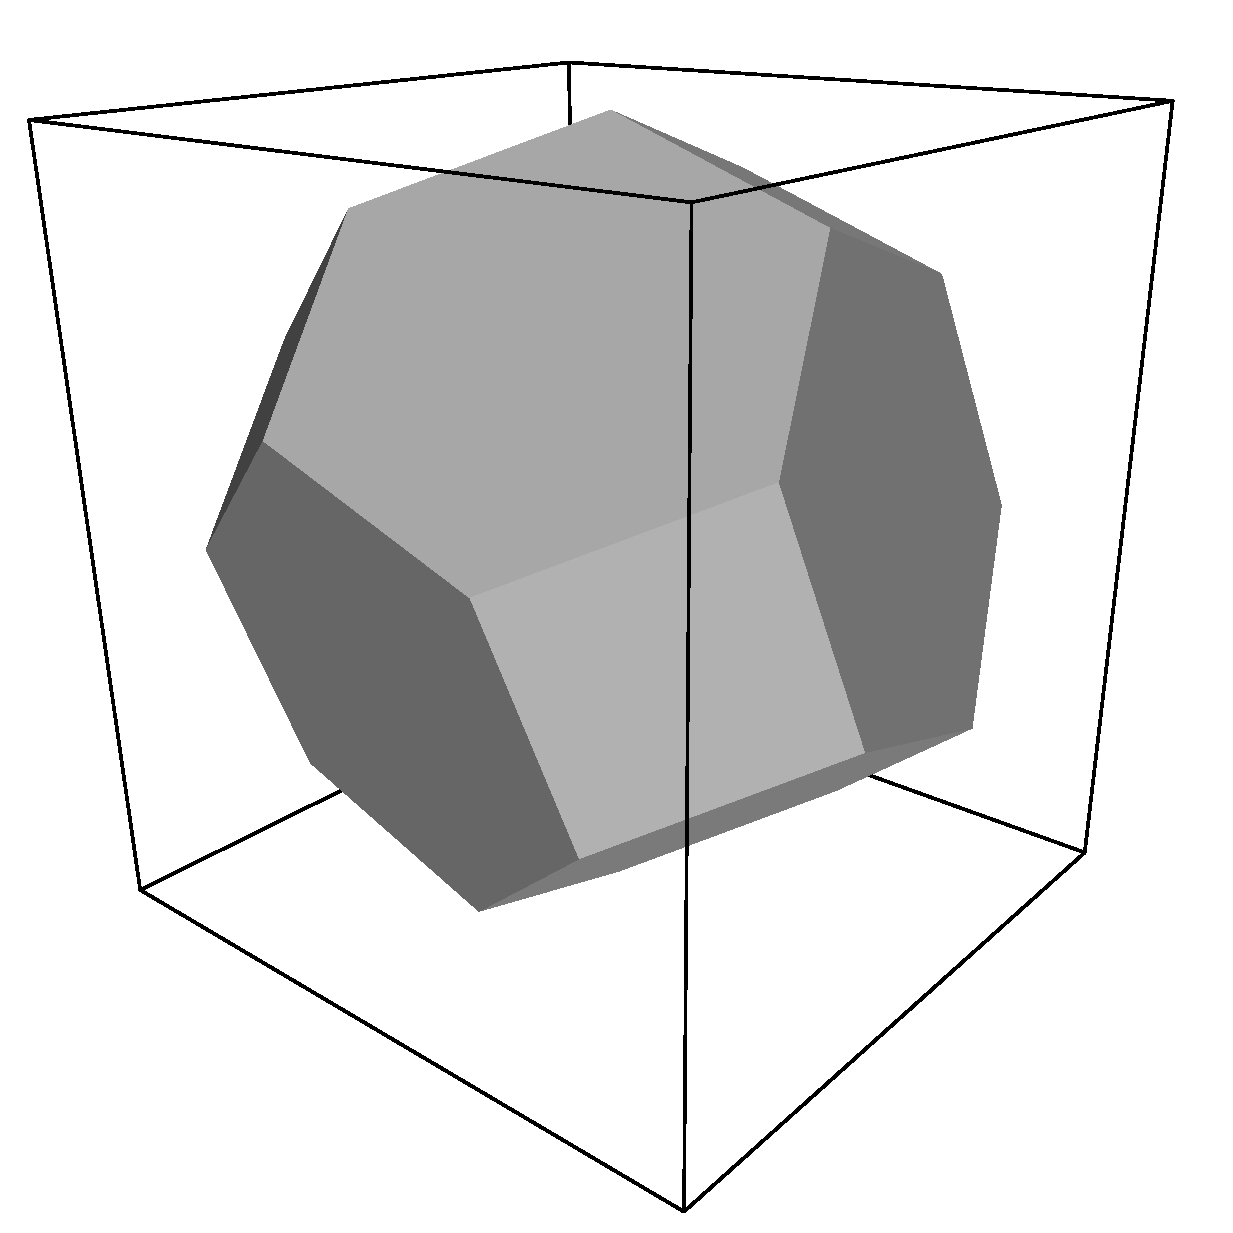
\includegraphics[width=5cm]{plots/truncoct}
}
\caption {A rhombic dodecahedron and truncated octahedron
(arbitrary orientations).}
\label{fig:boxshapes}
\end{figure}

\subsection{Some useful box types}
\begin{table}
\centerline{
\begin{tabular}{|c|c|c|ccc|ccc|}
\dline
box type & image & box & \multicolumn{3}{c|}{box vectors} & \multicolumn{3}{c|}{box vector angles} \\
 & distance & volume & ~{\bf a}~ & {\bf b} & {\bf c} &
   $\angle{\bf bc}$ & $\angle{\bf ac}$ & $\angle{\bf ab}$ \\
\dline
             &     &       & $d$ & 0              & 0              & & & \\
cubic        & $d$ & $d^3$ & 0   & $d$            & 0              & $90^\circ$ & $90^\circ$ & $90^\circ$ \\
             &     &       & 0   & 0              & $d$            & & & \\
\hline
rhombic      &     &       & $d$ & 0              & $\frac{1}{2}\,d$ & & & \\
dodecahedron & $d$ & $\frac{1}{2}\sqrt{2}\,d^3$ & 0   & $d$            & $\frac{1}{2}\,d$ & $60^\circ$ & $60^\circ$ & $90^\circ$ \\
(xy-square)  &     & $0.707\,d^3$ & 0   & 0              & $\frac{1}{2}\sqrt{2}\,d$ & & & \\
\hline
rhombic      &     &       & $d$ & $\frac{1}{2}\,d$ & $\frac{1}{2}\,d$ & & & \\
dodecahedron & $d$ & $\frac{1}{2}\sqrt{2}\,d^3$ & 0 & $\frac{1}{2}\sqrt{3}\,d$ & $\frac{1}{6}\sqrt{3}\,d$ & $60^\circ$ & $60^\circ$ & $60^\circ$ \\
(xy-hexagon) &     & $0.707\,d^3$ & 0   & 0              & $\frac{1}{3}\sqrt{6}\,d$ & & & \\
\hline
truncated    &     &       & $d$ & $\frac{1}{3}\,d$ & $-\frac{1}{3}\,d$ & & &\\
octahedron   & $d$ & $\frac{4}{9}\sqrt{3}\,d^3$ & 0   & $\frac{2}{3}\sqrt{2}\,d$ & $\frac{1}{3}\sqrt{2}\,d$ & $71.53^\circ$ & $109.47^\circ$ & $71.53^\circ$ \\
             &     & $0.770\,d^3$ & 0   & 0              & $\frac{1}{3}\sqrt{6}\,d$ & & & \\
\dline
\end{tabular}
}
\caption{The cubic box, the rhombic \normindex{dodecahedron} and the truncated
\normindex{octahedron}.}
\label{tab:boxtypes}
\end{table}
The three most useful box types for simulations of solvated systems
are described in \tabref{boxtypes}.  The rhombic dodecahedron
(\figref{boxshapes}) is the smallest and most regular space-filling
unit cell. Each of the 12 image cells is at the same distance.  The
volume is 71\% of the volume of a cube having the same image
distance. This saves about 29\% of CPU-time when simulating a
spherical or flexible molecule in solvent. There are two different
orientations of a rhombic dodecahedron that satisfy equations
\ref{eqn:box_rot}, \ref{eqn:box_shift1} and \ref{eqn:box_shift2}.
The program {\tt editconf} produces the orientation
which has a square intersection with the xy-plane.  This orientation
was chosen because the first two box vectors coincide with the x and
y-axis, which is easier to comprehend. The other orientation can be
useful for simulations of membrane proteins. In this case the
cross-section with the xy-plane is a hexagon, which has an area which
is 14\% smaller than the area of a square with the same image
distance.  The height of the box ($c_z$) should be changed to obtain
an optimal spacing.  This box shape not only saves CPU time, it
also results in a more uniform arrangement of the proteins.

\subsection{Cut-off restrictions}
The \normindex{minimum image convention} implies that the cut-off radius used to
truncate non-bonded interactions may not exceed half the shortest box
vector:
\beq
\label{eqn:physicalrc}
  R_c < \half \min(\|{\bf a}\|,\|{\bf b}\|,\|{\bf c}\|),
\eeq
because otherwise more than one image would be within the cut-off distance 
of the force. When a macromolecule, such as a protein, is studied in
solution, this restriction alone is not sufficient: in principle, a single
solvent molecule should not be able
to `see' both sides of the macromolecule. This means that the length of
each box vector must exceed the length of the macromolecule in the
direction of that edge {\em plus} two times the cut-off radius $R_c$.
It is, however, common to compromise in this respect, and make the solvent 
layer somewhat smaller in order to reduce the computational cost.
For efficiency reasons the cut-off with triclinic boxes is more restricted.
For grid search the extra restriction is weak:
\beq
\label{eqn:gridrc}
R_c < \min(a_x,b_y,c_z)
\eeq
For simple search the extra restriction is stronger:
\beq
\label{eqn:simplerc}
R_c < \half \min(a_x,b_y,c_z)
\eeq

Each unit cell (cubic, rectangular or triclinic)
is surrounded by 26 translated images. A
particular image can therefore always be identified by an index pointing to one
of 27 {\em translation vectors} and constructed by applying a
translation with the indexed vector (see \ssecref{forces}).
Restriction (\ref{eqn:gridrc}) ensures that only 26 images need to be
considered.

%\ifthenelse{\equal{\gmxlite}{1}}{}{
\section{The group concept}
\label{sec:groupconcept}\index{group}
The {\gromacs} MD and analysis programs use user-defined {\em groups} of
atoms to perform certain actions on. The maximum number of groups is
256, but each atom can only belong to six different groups, one 
each of the following:
\begin{description}
\item[\swapindex{temperature-coupling}{group}]
The \normindex{temperature coupling} parameters (reference
temperature, time constant, number of degrees of freedom, see
\ssecref{update}) can be defined for each T-coupling group
separately. For example, in a solvated macromolecule the solvent (that
tends to generate more heating by force and integration errors) can be
coupled with a shorter time constant to a bath than is a macromolecule,
or a surface can be kept cooler than an adsorbing molecule. Many
different T-coupling groups may be defined. See also center of mass
groups below.

\item[\swapindex{freeze}{group}\index{frozen atoms}]
Atoms that belong to a freeze group are kept stationary in the
dynamics. This is useful during equilibration, {\eg} to avoid badly
placed solvent molecules giving unreasonable kicks to protein atoms,
although the same effect can also be obtained by putting a restraining
potential on the atoms that must be protected. The freeze option can
be used, if desired, on just one or two coordinates of an atom,
thereby freezing the atoms in a plane or on a line.  When an atom is
partially frozen, constraints will still be able to move it, even in a
frozen direction. A fully frozen atom can not be moved by constraints.
Many freeze groups can be defined.  Frozen coordinates are unaffected
by pressure scaling; in some cases this can produce unwanted results,
particularly when constraints are also used (in this case you will
get very large pressures). Accordingly, it is recommended to avoid
combining freeze groups with constraints and pressure coupling. For the
sake of equilibration it could suffice to start with freezing in a
constant volume simulation, and afterward use position restraints in
conjunction with constant pressure.

\item[\swapindex{accelerate}{group}]
On each atom in an ``accelerate group'' an acceleration
$\ve{a}^g$ is imposed. This is equivalent to an external
force. This feature makes it possible to drive the system into a
non-equilibrium state and enables the performance of 
\swapindex{non-equilibrium}{MD} and hence to obtain transport properties.

\item[\swapindex{energy-monitor}{group}]
Mutual interactions between all energy-monitor groups are compiled
during the simulation. This is done separately for Lennard-Jones and
Coulomb terms.  In principle up to 256 groups could be defined, but
that would lead to 256$\times$256 items! Better use this concept
sparingly.

All non-bonded interactions between pairs of energy-monitor groups can
be excluded\index{exclusions}
\ifthenelse{\equal{\gmxlite}{1}}
{.}
{(see details in the User Guide).}
Pairs of particles from excluded pairs of energy-monitor groups
are not put into the pair list.
This can result in a significant speedup
for simulations where interactions within or between parts of the system
are not required.

\item[\swapindex{center of mass}{group}\index{removing COM motion}]
In \gromacs\ the center of mass (COM) motion can be removed, for
either the complete system or for groups of atoms. The latter is
useful, {\eg} for systems where there is limited friction ({\eg} gas
systems) to prevent center of mass motion to occur. It makes sense to
use the same groups for temperature coupling and center of mass motion
removal.

\item[\swapindex{Compressed position output}{group}]

In order to further reduce the size of the compressed trajectory file
({\tt .xtc{\index{XTC}}} or {\tt .tng{\index{TNG}}}), it is possible
to store only a subset of all particles. All x-compression groups that
are specified are saved, the rest are not. If no such groups are
specified, than all atoms are saved to the compressed trajectory file.

\end{description}
The use of groups in {\gromacs} tools is described in
\secref{usinggroups}.
%} % Brace matches ifthenelse test for gmxlite

\section{Molecular Dynamics}
\label{sec:MD}
\begin{figure}
\begin{center}
\addtolength{\fboxsep}{0.5cm}
\begin{shadowenv}[12cm]
{\large \bf THE GLOBAL MD ALGORITHM}
\rule{\textwidth}{2pt} \\
{\bf 1. Input initial conditions}\\[2ex]
Potential interaction $V$ as a function of atom positions\\
Positions $\ve{r}$ of all atoms in the system\\
Velocities $\ve{v}$ of all atoms in the system \\
$\Downarrow$\\
\rule{\textwidth}{1pt}\\
{\bf repeat 2,3,4} for the required number of steps:\\
\rule{\textwidth}{1pt}\\
{\bf 2. Compute forces} \\[1ex]
The force on any atom  \\[1ex]
$\ve{F}_i = - \displaystyle\frac{\partial V}{\partial \ve{r}_i}$ \\[1ex]
is computed by calculating the force between non-bonded atom pairs: \\
$\ve{F}_i = \sum_j \ve{F}_{ij}$ \\
plus the forces due to bonded interactions (which may depend on 1, 2,
3, or 4 atoms), plus restraining and/or external forces. \\
The potential and kinetic energies and the pressure tensor may be computed. \\
$\Downarrow$\\
{\bf 3. Update configuration} \\[1ex]
The movement of the atoms is simulated by numerically solving Newton's
equations of motion \\[1ex]
$\displaystyle
\frac {\de^2\ve{r}_i}{\de t^2} = \frac{\ve{F}_i}{m_i} $ \\
or \\
$\displaystyle
\frac{\de\ve{r}_i}{\de t} = \ve{v}_i ; \;\;
\frac{\de\ve{v}_i}{\de t} = \frac{\ve{F}_i}{m_i} $ \\[1ex]
$\Downarrow$ \\
{\bf 4.} if required: {\bf Output step} \\
write positions, velocities, energies, temperature, pressure, etc. \\
\end{shadowenv}
\caption{The global MD algorithm}
\label{fig:global}
\end{center}
\end{figure}
A global flow scheme for MD is given in \figref{global}. Each
MD or  EM run requires as input a set of initial coordinates and --
optionally -- initial velocities of all particles involved. This
chapter does not describe how these are obtained; for the setup of an
actual MD run check the online manual at {\wwwpage}.

\subsection{Initial conditions}
\subsubsection{Topology and force field}
The system topology, including a description of the force field, must
be read in.
\ifthenelse{\equal{\gmxlite}{1}}
{.}
{Force fields and topologies are described in \chref{ff}
and \ref{ch:top}, respectively.}
All this information is static; it is never modified during the run.

\subsubsection{Coordinates and velocities}
\begin{figure}
\centerline{\includegraphics[width=8cm]{plots/maxwell}}
\caption{A Maxwell-Boltzmann velocity distribution, generated from 
    random numbers.}
\label{fig:maxwell}
\end{figure}

Then, before a run starts, the box size and the coordinates and
velocities of  all particles are required. The box size and shape is 
determined by three vectors (nine numbers) $\ve{b}_1, \ve{b}_2, \ve{b}_3$, 
which represent the three basis vectors of the periodic box.

If the run starts at $t=t_0$, the coordinates at $t=t_0$ must be
known. The {\em leap-frog algorithm}, the default algorithm used to 
update the time step with $\Dt$ (see \ssecref{update}), also requires 
that the velocities at $t=t_0 - \hDt$ are known. If velocities are not 
available, the program can generate initial atomic velocities 
$v_i, i=1\ldots 3N$ with a \index{Maxwell-Boltzmann distribution} 
(\figref{maxwell}) at a given absolute temperature $T$:
\beq 
p(v_i) = \sqrt{\frac{m_i}{2 \pi kT}}\exp\left(-\frac{m_i v_i^2}{2kT}\right)
\eeq
where $k$ is Boltzmann's constant (see \chref{defunits}).
To accomplish this, normally distributed random numbers are generated
by adding twelve random numbers $R_k$ in the range $0 \le R_k < 1$ and
subtracting 6.0 from their sum. The result is then multiplied by the
standard deviation of the velocity distribution $\sqrt{kT/m_i}$. Since
the resulting total energy will not correspond exactly to the required
temperature $T$, a correction is made: first the center-of-mass motion
is removed and then all velocities are scaled so that the total
energy corresponds exactly to $T$ (see \eqnref{E-T}). 
% Why so complicated? What's wrong with Box-Mueller transforms?

\subsubsection{Center-of-mass motion\index{removing COM motion}}
The \swapindex{center-of-mass}{velocity} is normally set to zero at
every step; there is (usually) no net external force acting on the
system and the center-of-mass velocity should remain constant. In
practice, however, the update algorithm introduces a very slow change in
the center-of-mass velocity, and therefore in the total kinetic energy of
the system -- especially when temperature coupling is used. If such
changes are not quenched, an appreciable center-of-mass motion
can develop in long runs, and the temperature will be
significantly misinterpreted. Something similar may happen due to overall
rotational motion, but only when an isolated cluster is simulated. In
periodic systems with filled boxes, the overall rotational motion is
coupled to other degrees of freedom and does not cause such problems.


\subsection{Neighbor searching\swapindexquiet{neighbor}{searching}}
\label{subsec:ns}
As mentioned in \chref{ff}, internal forces are
either generated from fixed (static) lists, or from dynamic lists.
The latter consist of non-bonded interactions between any pair of particles.
When calculating the non-bonded forces, it is convenient to have all
particles in a rectangular box.
As shown in \figref{pbc}, it is possible to transform a
triclinic box into a rectangular box.
The output coordinates are always in a rectangular box, even when a
dodecahedron or triclinic box was used for the simulation.
Equation \ref{eqn:box_rot} ensures that we can reset particles
in a rectangular box by first shifting them with
box vector ${\bf c}$, then with ${\bf b}$ and finally with ${\bf a}$.
Equations \ref{eqn:box_shift2}, \ref{eqn:physicalrc} and \ref{eqn:gridrc}
ensure that we can find the 14 nearest triclinic images within
a linear combination that does not involve multiples of box vectors.

\subsubsection{Pair lists generation}
The non-bonded pair forces need to be calculated only for those pairs
$i,j$  for which the distance $r_{ij}$ between $i$ and the 
\swapindex{nearest}{image} 
of $j$ is less than a given cut-off radius $R_c$. Some of the particle
pairs that fulfill this criterion are excluded, when their interaction
is already fully accounted for by bonded interactions.  {\gromacs}
employs a {\em pair list} that contains those particle pairs for which
non-bonded forces must be calculated.  The pair list contains particles
$i$, a displacement vector for particle $i$, and all particles $j$ that
are within \verb'rlist' of this particular image of particle $i$.  The
list is updated every \verb'nstlist' steps.

To make the \normindex{neighbor list}, all particles that are close
({\ie} within the neighbor list cut-off) to a given particle must be found.
This searching, usually called neighbor search (NS) or pair search,
involves periodic boundary conditions and determining the {\em image}
(see \secref{pbc}). The search algorithm is $O(N)$, although a simpler
$O(N^2)$ algorithm is still available under some conditions.

\subsubsection{\normindex{Cut-off schemes}: group versus Verlet}
From version 4.6, {\gromacs} supports two different cut-off scheme
setups: the original one based on particle groups and one using a Verlet
buffer. There are some important differences that affect results,
performance and feature support. The group scheme can be made to work
(almost) like the Verlet scheme, but this will lead to a decrease in
performance. The group scheme is especially fast for water molecules,
which are abundant in many simulations, but on the most recent x86
processors, this advantage is negated by the better instruction-level
parallelism available in the Verlet-scheme implementation. The group
scheme is deprecated in version 5.0, and will be removed in a future
version. For practical details of choosing and setting up
cut-off schemes, please see the User Guide.

In the group scheme, a neighbor list is generated consisting of pairs
of groups of at least one particle. These groups were originally
\swapindex{charge}{group}s \ifthenelse{\equal{\gmxlite}{1}}{}{(see
  \secref{chargegroup})}, but with a proper treatment of long-range
electrostatics, performance in unbuffered simulations is their only advantage. A pair of groups
is put into the neighbor list when their center of geometry is within
the cut-off distance. Interactions between all particle pairs (one from
each charge group) are calculated for a certain number of MD steps,
until the neighbor list is updated. This setup is efficient, as the
neighbor search only checks distance between charge-group pair, not
particle pairs (saves a factor of $3 \times 3 = 9$ with a three-particle water
model) and the non-bonded force kernels can be optimized for, say, a
water molecule ``group''. Without explicit buffering, this setup leads
to energy drift as some particle pairs which are within the cut-off don't
interact and some outside the cut-off do interact. This can be caused
by
\begin{itemize}
\item particles moving across the cut-off between neighbor search steps, and/or
\item for charge groups consisting of more than one particle, particle pairs
  moving in/out of the cut-off when their charge group center of
  geometry distance is outside/inside of the cut-off.
\end{itemize}
Explicitly adding a buffer to the neighbor list will remove such
artifacts, but this comes at a high computational cost. How severe the
artifacts are depends on the system, the properties in which you are
interested, and the cut-off setup.

The Verlet cut-off scheme uses a buffered pair list by default. It
also uses clusters of particles, but these are not static as in the group
scheme. Rather, the clusters are defined spatially and consist of 4 or
8 particles, which is convenient for stream computing, using e.g. SSE, AVX
or CUDA on GPUs. At neighbor search steps, a pair list is created
with a Verlet buffer, ie. the pair-list cut-off is larger than the
interaction cut-off. In the non-bonded kernels, interactions are only
computed when a particle pair is within the cut-off distance at that
particular time step. This ensures that as particles move between pair
search steps, forces between nearly all particles within the cut-off
distance are calculated. We say {\em nearly} all particles, because
{\gromacs} uses a fixed pair list update frequency for
efficiency. A particle-pair, whose distance was outside the cut-off,
could possibly move enough during this fixed number of
steps that its distance is now within the cut-off. This
small chance results in a small energy drift, and the size of the
chance depends on the temperature. When temperature
coupling is used, the buffer size can be determined automatically,
given a certain tolerance on the energy drift.

The Verlet cut-off scheme is implemented in a very efficient fashion
based on clusters of particles. The simplest example is a cluster size
of 4 particles. The pair list is then constructed based on cluster
pairs. The cluster-pair search is much faster searching based on
particle pairs, because $4 \times 4 = 16$ particle pairs are put in
the list at once. The non-bonded force calculation kernel can then
calculate many particle-pair interactions at once, which maps nicely
to SIMD or SIMT units on modern hardware, which can perform multiple
floating operations at once. These non-bonded kernels
are much faster than the kernels used in the group scheme for most
types of systems, particularly on newer hardware.

\ifthenelse{\equal{\gmxlite}{1}}{}{
\subsubsection{Energy drift and pair-list buffering}
For a canonical (NVT) ensemble, the average energy error caused by
diffusion of $j$ particles from outside the pair-list cut-off
$r_\ell$ to inside the interaction cut-off $r_c$ over the lifetime
of the list can be determined from the atomic
displacements and the shape of the potential at the cut-off.
%Since we are interested in the small drift regime, we will assume
%#that atoms will only move within the cut-off distance in the last step,
%$n_\mathrm{ps}-1$, of the pair list update interval $n_\mathrm{ps}$.
%Over this number of steps the displacment of an atom with mass $m$
The displacement distribution along one dimension for a freely moving
particle with mass $m$ over time $t$ at temperature $T$ is
a Gaussian $G(x)$
of zero mean and variance $\sigma^2 = t^2 k_B T/m$. For the distance
between two particles, the variance changes to $\sigma^2 = \sigma_{12}^2 =
t^2 k_B T(1/m_1+1/m_2)$. Note that in practice particles usually
interact with other particles over time $t$ and therefore the real
displacement distribution is much narrower.  Given a non-bonded
interaction cut-off distance of $r_c$ and a pair-list cut-off
$r_\ell=r_c+r_b$ for $r_b$ the Verlet buffer size, we can then
write the average energy error after time $t$ for all missing pair
interactions between a single $i$ particle of type 1 surrounded
by all $j$ particles that are of type 2 with number density $\rho_2$,
when the inter-particle distance changes from $r_0$ to $r_t$, as:
\beq
\langle \Delta V \rangle =
\int_{0}^{r_c} \int_{r_\ell}^\infty 4 \pi r_0^2 \rho_2 V(r_t) G\!\left(\frac{r_t-r_0}{\sigma}\right) d r_0\, d r_t
\eeq
To evaluate this analytically, we need to make some approximations. First we replace $V(r_t)$ by a Taylor expansion around $r_c$, then we can move the lower bound of the integral over $r_0$ to $-\infty$ which will simplify the result:
\begin{eqnarray}
\langle \Delta V \rangle &\approx&
\int_{-\infty}^{r_c} \int_{r_\ell}^\infty 4 \pi r_0^2 \rho_2 \Big[ V'(r_c) (r_t - r_c) +
\nonumber\\
& &
\phantom{\int_{-\infty}^{r_c} \int_{r_\ell}^\infty 4 \pi r_0^2 \rho_2 \Big[}
V''(r_c)\frac{1}{2}(r_t - r_c)^2 +
\nonumber\\
& &
\phantom{\int_{-\infty}^{r_c} \int_{r_\ell}^\infty 4 \pi r_0^2 \rho_2 \Big[}
  V'''(r_c)\frac{1}{6}(r_t - r_c)^3 +
  \nonumber\\
& &
\phantom{\int_{-\infty}^{r_c} \int_{r_\ell}^\infty 4 \pi r_0^2 \rho_2 \Big[}
  O \! \left((r_t - r_c)^4 \right)\Big] G\!\left(\frac{r_t-r_0}{\sigma}\right) d r_0 \, d r_t
\end{eqnarray}
Replacing the factor $r_0^2$ by $(r_\ell + \sigma)^2$, which results in a slight overestimate, allows us to calculate the integrals analytically:
\begin{eqnarray}
\langle \Delta V \rangle \!
&\approx&
4 \pi (r_\ell+\sigma)^2 \rho_2
\int_{-\infty}^{r_c} \int_{r_\ell}^\infty \Big[ V'(r_c) (r_t - r_c) +
\nonumber\\
& &
\phantom{4 \pi (r_\ell+\sigma)^2 \rho_2 \int_{-\infty}^{r_c} \int_{r_\ell}^\infty \Big[}
V''(r_c)\frac{1}{2}(r_t - r_c)^2 +
\nonumber\\
& &
\phantom{4 \pi (r_\ell+\sigma)^2 \rho_2 \int_{-\infty}^{r_c} \int_{r_\ell}^\infty \Big[}
V'''(r_c)\frac{1}{6}(r_t - r_c)^3 \Big] G\!\left(\frac{r_t-r_0}{\sigma}\right)
d r_0 \, d r_t\\
&=&
4 \pi (r_\ell+\sigma)^2 \rho_2 \bigg\{
\frac{1}{2}V'(r_c)\left[r_b \sigma G\!\left(\frac{r_b}{\sigma}\right) - (r_b^2+\sigma^2)E\!\left(\frac{r_b}{\sigma}\right) \right] +
\nonumber\\
& &
\phantom{4 \pi (r_\ell+\sigma)^2 \rho_2 \bigg\{ }
\frac{1}{6}V''(r_c)\left[ \sigma(r_b^2+2\sigma^2) G\!\left(\frac{r_b}{\sigma}\right) - r_b(r_b^2+3\sigma^2 ) E\!\left(\frac{r_b}{\sigma}\right) \right] +
\nonumber\\
& &
\phantom{4 \pi (r_\ell+\sigma)^2 \rho_2 \bigg\{ }
\frac{1}{24}V'''(r_c)\bigg[ r_b\sigma(r_b^2+5\sigma^2) G\!\left(\frac{r_b}{\sigma}\right)
\nonumber\\
& &
\phantom{4 \pi (r_\ell+\sigma)^2 \rho_2 \bigg\{ \frac{1}{24}V'''(r_c)\bigg[ }
 - (r_b^4+6r_b^2\sigma^2+3\sigma^4 ) E\!\left(\frac{r_b}{\sigma}\right) \bigg]
\bigg\}
\end{eqnarray}

where $G(x)$ is a Gaussian distribution with 0 mean and unit variance and
$E(x)=\frac{1}{2}\mathrm{erfc}(x/\sqrt{2})$. We always want to achieve
small energy error, so $\sigma$ will be small compared to both $r_c$
and $r_\ell$, thus the approximations in the equations above are good,
since the Gaussian distribution decays rapidly. The energy error needs
to be averaged over all particle pair types and weighted with the
particle counts. In {\gromacs} we don't allow cancellation of error
between pair types, so we average the absolute values. To obtain the
average energy error per unit time, it needs to be divided by the
neighbor-list life time $t = ({\tt nstlist} - 1)\times{\tt dt}$. The
function can not be inverted analytically, so we use bisection to
obtain the buffer size $r_b$ for a target drift.  Again we note that
in practice the error we usually be much smaller than this estimate,
as in the condensed phase particle displacements will be much smaller
than for freely moving particles, which is the assumption used here.

When (bond) constraints are present, some particles will have fewer
degrees of freedom. This will reduce the energy errors. For simplicity,
we only consider one constraint per particle, the heaviest particle
in case a particle is involved in multiple constraints.
This simplification overestimates the displacement. The motion of
a constrained particle is a superposition of the 3D motion of the
center of mass of both particles and a 2D rotation around the center of mass.
The displacement in an arbitrary direction of a particle with 2 degrees
of freedom is not Gaussian, but rather follows the complementary error
function:
\beq
\frac{\sqrt{\pi}}{2\sqrt{2}\sigma}\,\mathrm{erfc}\left(\frac{|r|}{\sqrt{2}\,\sigma}\right)
\label{eqn:2D_disp}
\eeq
where $\sigma^2$ is again $t^2 k_B T/m$.  This distribution can no
longer be integrated analytically to obtain the energy error. But we
can generate a tight upper bound using a scaled and shifted Gaussian
distribution (not shown). This Gaussian distribution can then be used
to calculate the energy error as described above. The rotation displacement
around the center of mass can not be more than the length of the arm.
To take this into account, we scale $\sigma$ in \eqnref{2D_disp} (details
not presented here) to obtain an overestimate of the real displacement.
This latter effect significantly reduces the buffer size for longer
neighborlist lifetimes in e.g. water, as constrained hydrogens are by far
the fastest particles, but they can not move further than 0.1 nm
from the heavy atom they are connected to.


There is one important implementation detail that reduces the energy
errors caused by the finite Verlet buffer list size. The derivation
above assumes a particle pair-list. However, the {\gromacs}
implementation uses a cluster pair-list for efficiency. The pair list
consists of pairs of clusters of 4 particles in most cases, also
called a $4 \times 4$ list, but the list can also be $4 \times 8$ (GPU
CUDA kernels and AVX 256-bit single precision kernels) or $4 \times 2$
(SSE double-precision kernels). This means that the pair-list is
effectively much larger than the corresponding $1 \times 1$ list. Thus
slightly beyond the pair-list cut-off there will still be a large
fraction of particle pairs present in the list. This fraction can be
determined in a simulation and accurately estimated under some
reasonable assumptions. The fraction decreases with increasing
pair-list range, meaning that a smaller buffer can be used. For
typical all-atom simulations with a cut-off of 0.9 nm this fraction is
around 0.9, which gives a reduction in the energy errors of a factor of
10. This reduction is taken into account during the automatic Verlet
buffer calculation and results in a smaller buffer size.

\begin{figure}
\centerline{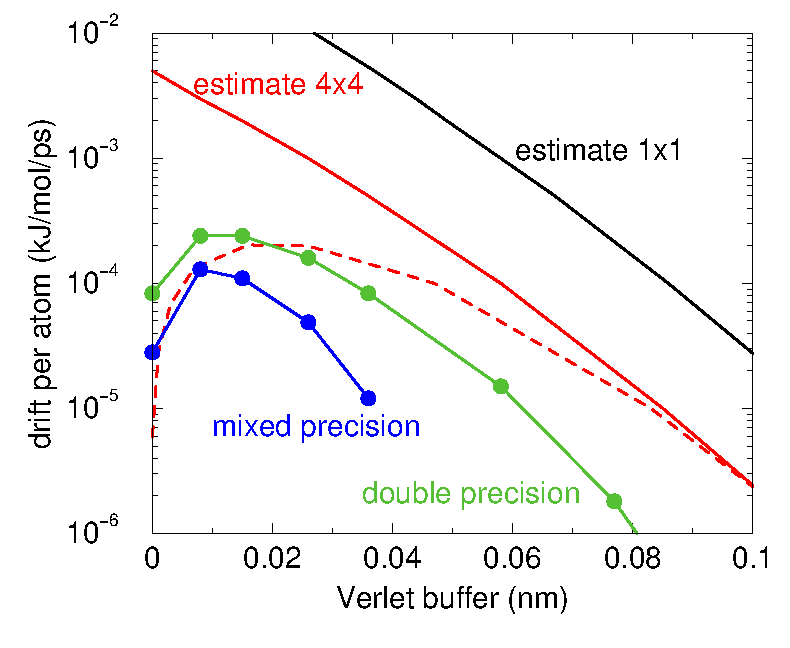
\includegraphics[width=9cm]{plots/verlet-drift}}
\caption {Energy drift per atom for an SPC/E water system at 300K with
  a time step of 2 fs and a pair-list update period of 10 steps
  (pair-list life time: 18 fs). PME was used with {\tt ewald-rtol} set
  to 10$^{-5}$; this parameter affects the shape of the potential at
  the cut-off. Error estimates due to finite Verlet buffer size are
  shown for a $1 \times 1$ atom pair list and $4 \times 4$ atom pair
  list without and with (dashed line) cancellation of positive and
  negative errors. Real energy drift is shown for simulations using
  double- and mixed-precision settings. Rounding errors in the SETTLE
  constraint algorithm from the use of single precision causes
  the drift to become negative
  at large buffer size. Note that at zero buffer size, the real drift
  is small because positive (H-H) and negative (O-H) energy errors
  cancel.}
\label{fig:verletdrift}
\end{figure}

In \figref{verletdrift} one can see that for small buffer sizes the drift
of the total energy is much smaller than the pair energy error tolerance,
due to cancellation of errors. For larger buffer size, the error estimate
is a factor of 6 higher than drift of the total energy, or alternatively
the buffer estimate is 0.024 nm too large. This is because the protons
don't move freely over 18 fs, but rather vibrate.
%At a buffer size of zero there is cancellation of
%drift due to repulsive (H-H) and attractive (O-H) interactions.

\subsubsection{Cut-off artifacts and switched interactions}
With the Verlet scheme, the pair potentials are shifted to be zero at
the cut-off, which makes the potential the integral of the force.
This is only possible in the group scheme if the shape of the potential
is such that its value is zero at the cut-off distance.
However, there can still be energy drift when the
forces are non-zero at the cut-off. This effect is extremely small and
often not noticeable, as other integration errors (e.g. from constraints)
may dominate. To
completely avoid cut-off artifacts, the non-bonded forces can be
switched exactly to zero at some distance smaller than the neighbor
list cut-off (there are several ways to do this in {\gromacs}, see
\secref{mod_nb_int}). One then has a buffer with the size equal to the
neighbor list cut-off less the longest interaction cut-off.

} % Brace matches ifthenelse test for gmxlite

\subsubsection{Simple search\swapindexquiet{simple}{search}}
Due to \eqnsref{box_rot}{simplerc}, the vector $\rvij$
connecting images within the cut-off $R_c$ can be found by constructing:
\bea
\ve{r}'''   & = & \ve{r}_j-\ve{r}_i \\
\ve{r}''    & = & \ve{r}''' - {\bf c}*\verb'round'(r'''_z/c_z) \\
\ve{r}'     & = & \ve{r}'' - {\bf b}*\verb'round'(r''_y/b_y) \\
\ve{r}_{ij} & = & \ve{r}' - {\bf a}*\verb'round'(r'_x/a_x)
\eea
When distances between two particles in a triclinic box are needed
that do not obey \eqnref{box_rot},
many shifts of combinations of box vectors need to be considered to find
the nearest image.

\ifthenelse{\equal{\gmxlite}{1}}{}{

\begin{figure}
\centerline{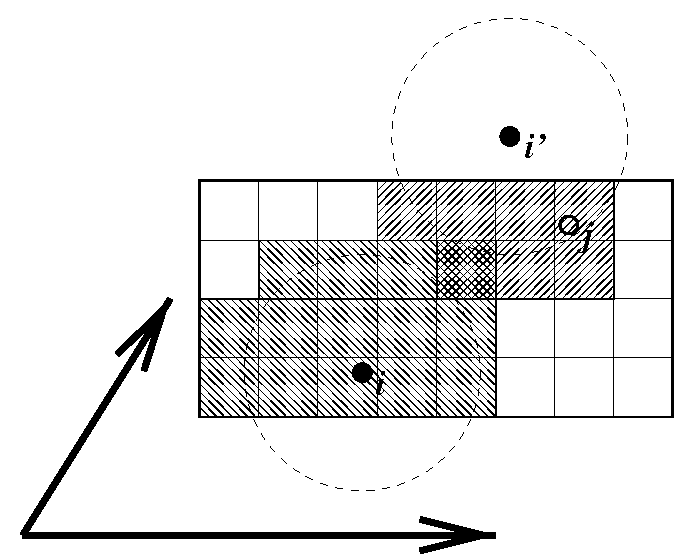
\includegraphics[width=8cm]{plots/nstric}}
\caption {Grid search in two dimensions. The arrows are the box vectors.}
\label{fig:grid}
\end{figure}

\subsubsection{Grid search\swapindexquiet{grid}{search}}
\label{sec:nsgrid}
The grid search is schematically depicted in \figref{grid}.  All
particles are put on the {\nsgrid}, with the smallest spacing $\ge$
$R_c/2$ in each of the directions.  In the direction of each box
vector, a particle $i$ has three images. For each direction the image
may be -1,0 or 1, corresponding to a translation over -1, 0 or +1 box
vector. We do not search the surrounding {\nsgrid} cells for neighbors
of $i$ and then calculate the image, but rather construct the images
first and then search neighbors corresponding to that image of $i$.
As \figref{grid} shows, some grid cells may be searched more than once
for different images of $i$. This is not a problem, since, due to the
minimum image convention, at most one image will ``see'' the
$j$-particle.  For every particle, fewer than 125 (5$^3$) neighboring
cells are searched.  Therefore, the algorithm scales linearly with the
number of particles.  Although the prefactor is large, the scaling
behavior makes the algorithm far superior over the standard $O(N^2)$
algorithm when there are more than a few hundred particles.  The
grid search is equally fast for rectangular and triclinic boxes.  Thus
for most protein and peptide simulations the rhombic dodecahedron will
be the preferred box shape.
} % Brace matches ifthenelse test for gmxlite

\ifthenelse{\equal{\gmxlite}{1}}{}{
\subsubsection{Charge groups}
\label{sec:chargegroup}\swapindexquiet{charge}{group}%
Charge groups were originally introduced to reduce cut-off artifacts
of Coulomb interactions. When a plain cut-off is used, significant
jumps in the potential and forces arise when atoms with (partial) charges
move in and out of the cut-off radius. When all chemical moieties have
a net charge of zero, these jumps can be reduced by moving groups
of atoms with net charge zero, called charge groups, in and
out of the neighbor list. This reduces the cut-off effects from
the charge-charge level to the dipole-dipole level, which decay
much faster. With the advent of full range electrostatics methods,
such as particle-mesh Ewald (\secref{pme}), the use of charge groups is
no longer required for accuracy. It might even have a slight negative effect
on the accuracy or efficiency, depending on how the neighbor list is made
and the interactions are calculated.

But there is still an important reason for using ``charge groups'': efficiency with the group cut-off scheme.
Where applicable, neighbor searching is carried out on the basis of
charge groups which are defined in the molecular topology.
If the nearest image distance between the {\em
geometrical centers} of the atoms of two charge groups is less than
the cut-off radius, all atom pairs between the charge groups are
included in the pair list.
The neighbor searching for a water system, for instance,
is $3^2=9$ times faster when each molecule is treated as a charge group.
Also the highly optimized water force loops (see \secref{waterloops})
only work when all atoms in a water molecule form a single charge group.
Currently the name {\em neighbor-search group} would be more appropriate,
but the name charge group is retained for historical reasons.
When developing a new force field, the advice is to use charge groups
of 3 to 4 atoms for optimal performance. For all-atom force fields
this is relatively easy, as one can simply put hydrogen atoms, and in some
case oxygen atoms, in the same charge group as the heavy atom they
are connected to; for example: CH$_3$, CH$_2$, CH, NH$_2$, NH, OH, CO$_2$, CO.

With the Verlet cut-off scheme, charge groups are ignored.

} % Brace matches ifthenelse test for gmxlite

\subsection{Compute forces}
\label{subsec:forces}

\subsubsection{Potential energy}
When forces are computed, the \swapindex{potential}{energy} of each
interaction term is computed as well. The total potential energy is
summed for various contributions, such as Lennard-Jones, Coulomb, and
bonded terms. It is also possible to compute these contributions for
{\em energy-monitor groups} of atoms that are separately defined (see
\secref{groupconcept}).

\subsubsection{Kinetic energy and temperature}
The \normindex{temperature} is given by the total
\swapindex{kinetic}{energy} of the $N$-particle system:
\beq
E_{kin} = \half \sum_{i=1}^N m_i v_i^2
\eeq
From this the absolute temperature $T$ can be computed using:
\beq
\half N_{\mathrm{df}} kT = E_{\mathrm{kin}}
\label{eqn:E-T}
\eeq
where $k$ is Boltzmann's constant and $N_{df}$ is the number of
degrees of freedom which can be computed from:
\beq
N_{\mathrm{df}}  ~=~     3 N - N_c - N_{\mathrm{com}}
\eeq
Here $N_c$ is the number of {\em \normindex{constraints}} imposed on the system.
When performing molecular dynamics $N_{\mathrm{com}}=3$ additional degrees of
freedom must be removed, because the three
center-of-mass velocities are constants of the motion, which are usually
set to zero. When simulating in vacuo, the rotation around the center of mass
can also be removed, in this case $N_{\mathrm{com}}=6$.
When more than one temperature-coupling group\index{temperature-coupling group} is used, the number of degrees
of freedom for group $i$ is:
\beq
N^i_{\mathrm{df}}  ~=~  (3 N^i - N^i_c) \frac{3 N - N_c - N_{\mathrm{com}}}{3 N - N_c}
\eeq

The kinetic energy can also be written as a tensor, which is necessary
for pressure calculation in a triclinic system, or systems where shear
forces  are imposed:
\beq
{\bf E}_{\mathrm{kin}} = \half \sum_i^N m_i \vvi \otimes \vvi
\eeq

\subsubsection{Pressure and virial}
The \normindex{pressure} 
tensor {\bf P} is calculated from the difference between 
kinetic energy $E_{\mathrm{kin}}$ and the \normindex{virial} ${\bf \Xi}$:
\beq
{\bf P} = \frac{2}{V} ({\bf E}_{\mathrm{kin}}-{\bf \Xi})
\label{eqn:P}
\eeq
where $V$ is the volume of the computational box. 
The scalar pressure $P$, which can be used for pressure coupling in the case
of isotropic systems, is computed as:
\beq
P       = {\rm trace}({\bf P})/3
\eeq

The virial ${\bf \Xi}$ tensor is defined as:
\beq
{\bf \Xi} = -\half \sum_{i<j} \rvij \otimes \Fvij 
\label{eqn:Xi}
\eeq

\ifthenelse{\equal{\gmxlite}{1}}{}{
The {\gromacs} implementation of the virial computation is described
in \secref{virial}.
} % Brace matches ifthenelse test for gmxlite


\subsection{The \swapindex{leap-frog}{integrator}}
\label{subsec:update}
\begin{figure}
\centerline{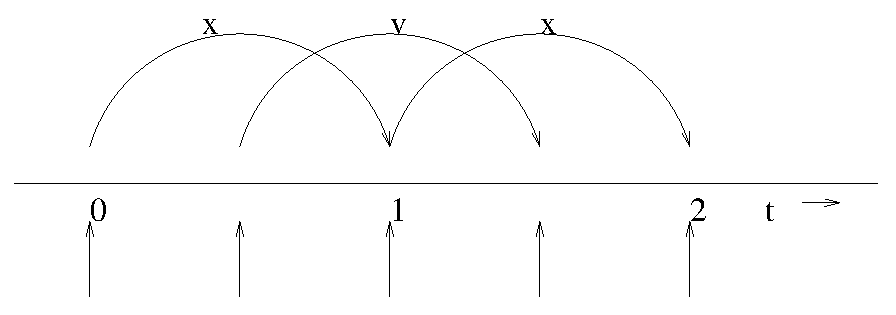
\includegraphics[width=8cm]{plots/leapfrog}}
\caption[The Leap-Frog integration method.]{The Leap-Frog integration method. The algorithm is called Leap-Frog because $\ve{r}$ and $\ve{v}$ are leaping
like  frogs over each other's backs.}
\label{fig:leapfrog}
\end{figure}

The default MD integrator in {\gromacs} is the so-called {\em leap-frog} 
algorithm~\cite{Hockney74} for the integration of the equations of
motion.  When extremely accurate integration with temperature
and/or pressure coupling is required, the velocity Verlet integrators
are also present and may be preferable (see \ssecref{vverlet}). The leap-frog
algorithm uses positions $\ve{r}$ at time $t$ and
velocities $\ve{v}$ at time $t-\hDt$; it updates positions and
velocities using the forces
$\ve{F}(t)$ determined by the positions at time $t$ using these relations:
\bea
\label{eqn:leapfrogv}
\ve{v}(t+\hDt)  &~=~&   \ve{v}(t-\hDt)+\frac{\Dt}{m}\ve{F}(t)   \\
\ve{r}(t+\Dt)   &~=~&   \ve{r}(t)+\Dt\ve{v}(t+\hDt)
\eea
The algorithm is visualized in \figref{leapfrog}.
It produces trajectories that are identical to the Verlet~\cite{Verlet67} algorithm,
whose position-update relation is
\beq
\ve{r}(t+\Dt)~=~2\ve{r}(t) - \ve{r}(t-\Dt) + \frac{1}{m}\ve{F}(t)\Dt^2+O(\Dt^4)
\eeq
The algorithm is of third order in $\ve{r}$ and is time-reversible.
See ref.~\cite{Berendsen86b} for the merits of this algorithm and comparison
with other time integration algorithms.

The \swapindex{equations of}{motion} are modified for temperature
coupling and pressure coupling, and extended to include the
conservation of constraints, all of which are described below.  

\subsection{The \swapindex{velocity Verlet}{integrator}}
\label{subsec:vverlet}
The velocity Verlet algorithm~\cite{Swope82} is also implemented in
{\gromacs}, though it is not yet fully integrated with all sets of
options.  In velocity Verlet, positions $\ve{r}$ and velocities
$\ve{v}$ at time $t$ are used to integrate the equations of motion;
velocities at the previous half step are not required.  \bea
\label{eqn:velocityverlet1}
\ve{v}(t+\hDt)  &~=~&   \ve{v}(t)+\frac{\Dt}{2m}\ve{F}(t)   \\
\ve{r}(t+\Dt)   &~=~&   \ve{r}(t)+\Dt\,\ve{v}(t+\hDt) \\
\ve{v}(t+\Dt)   &~=~&   \ve{v}(t+\hDt)+\frac{\Dt}{2m}\ve{F}(t+\Dt)
\eea
or, equivalently,
\bea
\label{eqn:velocityverlet2}
\ve{r}(t+\Dt)   &~=~&   \ve{r}(t)+ \Dt\,\ve{v} + \frac{\Dt^2}{2m}\ve{F}(t) \\
\ve{v}(t+\Dt)   &~=~&   \ve{v}(t)+ \frac{\Dt}{2m}\left[\ve{F}(t) + \ve{F}(t+\Dt)\right]
\eea
With no temperature or pressure coupling, and with {\em corresponding}
starting points, leap-frog and velocity Verlet will generate identical
trajectories, as can easily be verified by hand from the equations
above.  Given a single starting file with the {\em same} starting
point $\ve{x}(0)$ and $\ve{v}(0)$, leap-frog and velocity Verlet will
{\em not} give identical trajectories, as leap-frog will interpret the
velocities as corresponding to $t=-\hDt$, while velocity Verlet will
interpret them as corresponding to the timepoint $t=0$.

\subsection{Understanding reversible integrators: The Trotter decomposition}
To further understand the relationship between velocity Verlet and
leap-frog integration, we introduce the reversible Trotter formulation
of dynamics, which is also useful to understanding implementations of
thermostats and barostats in {\gromacs}.

A system of coupled, first-order differential equations can be evolved
from time $t = 0$ to time $t$ by applying the evolution operator
\bea
\Gamma(t) &=& \exp(iLt) \Gamma(0) \nonumber \\
iL &=& \dot{\Gamma}\cdot \nabla_{\Gamma},
\eea
where $L$ is the Liouville operator, and $\Gamma$ is the
multidimensional vector of independent variables (positions and
velocities).
A short-time approximation to the true operator, accurate at time $\Dt
= t/P$, is applied $P$ times in succession to evolve the system as
\beq
\Gamma(t) = \prod_{i=1}^P \exp(iL\Dt) \Gamma(0)
\eeq
For NVE dynamics, the Liouville operator is
\bea
iL = \sum_{i=1}^{N} \vv_i \cdot \nabla_{\rv_i} + \sum_{i=1}^N \frac{1}{m_i}\F(r_i) \cdot \nabla_{\vv_i}.
\eea
This can be split into two additive operators
\bea
iL_1 &=& \sum_{i=1}^N \frac{1}{m_i}\F(r_i) \cdot \nabla_{\vv_i} \nonumber \\
iL_2 &=& \sum_{i=1}^{N} \vv_i \cdot \nabla_{\rv_i} 
\eea
Then a short-time, symmetric, and thus reversible approximation of the true dynamics will be
\bea
\exp(iL\Dt) = \exp(iL_2\hDt) \exp(iL_1\Dt) \exp(iL_2\hDt) + \mathcal{O}(\Dt^3).
\label{eq:NVE_Trotter}
\eea
This corresponds to velocity Verlet integration.  The first
exponential term over $\hDt$ corresponds to a velocity half-step, the
second exponential term over $\Dt$ corresponds to a full velocity
step, and the last exponential term over $\hDt$ is the final velocity
half step.  For future times $t = n\Dt$, this becomes
\bea
\exp(iLn\Dt) &\approx&  \left(\exp(iL_2\hDt) \exp(iL_1\Dt) \exp(iL_2\hDt)\right)^n \nonumber \\
             &\approx&  \exp(iL_2\hDt) \bigg(\exp(iL_1\Dt) \exp(iL_2\Dt)\bigg)^{n-1} \nonumber \\
             &       &  \;\;\;\; \exp(iL_1\Dt) \exp(iL_2\hDt) 
\eea
This formalism allows us to easily see the difference between the
different flavors of Verlet integrators.  The leap-frog integrator can
be seen as starting with Eq.~\ref{eq:NVE_Trotter} with the
$\exp\left(iL_1 \dt\right)$ term, instead of the half-step velocity
term, yielding
\bea 
\exp(iLn\dt) &=& \exp\left(iL_1 \dt\right) \exp\left(iL_2 \Dt \right) + \mathcal{O}(\Dt^3).
\eea 
Here, the full step in velocity is between $t-\hDt$ and $t+\hDt$,
since it is a combination of the velocity half steps in velocity
Verlet. For future times $t = n\Dt$, this becomes
\bea 
\exp(iLn\dt) &\approx& \bigg(\exp\left(iL_1 \dt\right) \exp\left(iL_2 \Dt \right)  \bigg)^{n}.
\eea 
Although at first this does not appear symmetric, as long as the full velocity
step is between $t-\hDt$ and $t+\hDt$, then this is simply a way of
starting velocity Verlet at a different place in the cycle.

Even though the trajectory and thus potential energies are identical
between leap-frog and velocity Verlet, the kinetic energy and
temperature will not necessarily be the same.  Standard velocity
Verlet uses the velocities at the $t$ to calculate the kinetic energy
and thus the temperature only at time $t$; the kinetic energy is then a sum over all particles
\bea
KE_{\mathrm{full}}(t) &=& \sum_i \left(\frac{1}{2m_i}\ve{v}_i(t)\right)^2 \nonumber\\ 
      &=& \sum_i \frac{1}{2m_i}\left(\frac{1}{2}\ve{v}_i(t-\hDt)+\frac{1}{2}\ve{v}_i(t+\hDt)\right)^2,
\eea
with the square on the {\em outside} of the average.  Standard
leap-frog calculates the kinetic energy at time $t$ based on the
average kinetic energies at the timesteps $t+\hDt$ and $t-\hDt$, or
the sum over all particles
\bea
KE_{\mathrm{average}}(t) &=& \sum_i \frac{1}{2m_i}\left(\frac{1}{2}\ve{v}_i(t-\hDt)^2+\frac{1}{2}\ve{v}_i(t+\hDt)^2\right),
\eea
where the square is {\em inside} the average.

A non-standard variant of velocity Verlet which averages the kinetic
energies $KE(t+\hDt)$ and $KE(t-\hDt)$, exactly like leap-frog, is also
now implemented in {\gromacs} (as {\tt .mdp} file option {\tt md-vv-avek}).  Without
temperature and pressure coupling, velocity Verlet with
half-step-averaged kinetic energies and leap-frog will be identical up
to numerical precision.  For temperature- and pressure-control schemes,
however, velocity Verlet with half-step-averaged kinetic energies and
leap-frog will be different, as will be discussed in the section in
thermostats and barostats.

The half-step-averaged kinetic energy and temperature are slightly more
accurate for a given step size; the difference in average kinetic
energies using the half-step-averaged kinetic energies ({\em md} and
{\em md-vv-avek}) will be closer to the kinetic energy obtained in the
limit of small step size than will the full-step kinetic energy (using
{\em md-vv}).  For NVE simulations, this difference is usually not
significant, since the positions and velocities of the particles are
still identical; it makes a difference in the way the the temperature
of the simulations are {\em interpreted}, but {\em not} in the
trajectories that are produced.  Although the kinetic energy is more
accurate with the half-step-averaged method, meaning that it changes
less as the timestep gets large, it is also more noisy.  The RMS deviation
of the total energy of the system (sum of kinetic plus
potential) in the half-step-averaged kinetic energy case will be
higher (about twice as high in most cases) than the full-step kinetic
energy.  The drift will still be the same, however, as again, the
trajectories are identical.

For NVT simulations, however, there {\em will} be a difference, as
discussed in the section on temperature control, since the velocities
of the particles are adjusted such that kinetic energies of the
simulations, which can be calculated either way, reach the
distribution corresponding to the set temperature.  In this case, the
three methods will not give identical results.

Because the velocity and position are both defined at the same time
$t$ the velocity Verlet integrator can be used for some methods,
especially rigorously correct pressure control methods, that are not
actually possible with leap-frog.  The integration itself takes
negligibly more time than leap-frog, but twice as many communication
calls are currently required.  In most cases, and especially for large
systems where communication speed is important for parallelization and
differences between thermodynamic ensembles vanish in the $1/N$ limit,
and when only NVT ensembles are required, leap-frog will likely be the
preferred integrator.  For pressure control simulations where the fine
details of the thermodynamics are important, only velocity Verlet
allows the true ensemble to be calculated.  In either case, simulation
with double precision may be required to get fine details of
thermodynamics correct.

\subsection{Multiple time stepping}
Several other simulation packages uses multiple time stepping for
bonds and/or the PME mesh forces. In {\gromacs} we have not implemented
this (yet), since we use a different philosophy. Bonds can be constrained
(which is also a more sound approximation of a physical quantum
oscillator), which allows the smallest time step to be increased
to the larger one. This not only halves the number of force calculations,
but also the update calculations. For even larger time steps, angle vibrations
involving hydrogen atoms can be removed using virtual interaction
\ifthenelse{\equal{\gmxlite}{1}}
{sites,}
{sites (see \secref{rmfast}),}
which brings the shortest time step up to
PME mesh update frequency of a multiple time stepping scheme.

\subsection{Temperature coupling\index{temperature coupling}}
While direct use of molecular dynamics gives rise to the NVE (constant
number, constant volume, constant energy ensemble), most quantities
that we wish to calculate are actually from a constant temperature
(NVT) ensemble, also called the canonical ensemble. {\gromacs} can use
the {\em weak-coupling} scheme of Berendsen~\cite{Berendsen84},
stochastic randomization through the Andersen
thermostat~\cite{Andersen80}, the extended ensemble Nos{\'e}-Hoover
scheme~\cite{Nose84,Hoover85}, or a velocity-rescaling
scheme~\cite{Bussi2007a} to simulate constant temperature, with
advantages of each of the schemes laid out below.

There are several other reasons why it might be necessary to control
the temperature of the system (drift during equilibration, drift as a
result of force truncation and integration errors, heating due to
external or frictional forces), but this is not entirely correct to do
from a thermodynamic standpoint, and in some cases only masks the
symptoms (increase in temperature of the system) rather than the
underlying problem (deviations from correct physics in the dynamics).
For larger systems, errors in ensemble averages and structural
properties incurred by using temperature control to remove slow drifts
in temperature appear to be negligible, but no completely
comprehensive comparisons have been carried out, and some caution must
be taking in interpreting the results.

\subsubsection{Berendsen temperature coupling\pawsindexquiet{Berendsen}{temperature coupling}\index{weak coupling}}
The Berendsen algorithm mimics weak coupling with first-order 
kinetics to an external heat bath with given temperature $T_0$. 
See ref.~\cite{Berendsen91} for a comparison with the
Nos{\'e}-Hoover scheme. The effect of this algorithm is
that a deviation of the system temperature from $T_0$ is slowly
corrected according to:
\beq
\frac{\de T}{\de t} = \frac{T_0-T}{\tau}
\label{eqn:Tcoupling}
\eeq
which means that a temperature deviation decays exponentially with a
time constant $\tau$.
This method of coupling has the advantage that the strength of the
coupling can be varied and adapted to the user requirement: for
equilibration purposes the coupling time can be taken quite short
({\eg} 0.01 ps), but for reliable equilibrium runs it can be taken much
longer ({\eg} 0.5 ps) in which case it hardly influences the
conservative dynamics. 

The Berendsen thermostat suppresses the fluctuations of the kinetic
energy.  This means that one does not generate a proper canonical
ensemble, so rigorously, the sampling will be incorrect.  This
error scales with $1/N$, so for very large systems most ensemble
averages will not be affected significantly, except for the
distribution of the kinetic energy itself.  However, fluctuation
properties, such as the heat capacity, will be affected.  A similar
thermostat which does produce a correct ensemble is the velocity
rescaling thermostat~\cite{Bussi2007a} described below.

The heat flow into or out of the system is affected by scaling the
velocities of each particle every step, or every $n_\mathrm{TC}$ steps,
with a time-dependent factor $\lambda$, given by:
\beq 
\lambda = \left[ 1 + \frac{n_\mathrm{TC} \Delta t}{\tau_T}
\left\{\frac{T_0}{T(t -  \hDt)} - 1 \right\} \right]^{1/2}
\label{eqn:lambda}
\eeq
The parameter $\tau_T$ is close, but not exactly equal, to the time constant
$\tau$ of the temperature coupling (\eqnref{Tcoupling}):
\beq
\tau = 2 C_V \tau_T / N_{df} k
\eeq
where $C_V$ is the total heat capacity of the system, $k$ is Boltzmann's
constant, and $N_{df}$ is the total number of degrees of freedom. The
reason that $\tau \neq \tau_T$ is that the kinetic energy change
caused by scaling the velocities is partly redistributed between
kinetic and potential energy and hence the change in temperature is
less than the scaling energy.  In practice, the ratio $\tau / \tau_T$
ranges from 1 (gas) to 2 (harmonic solid) to 3 (water). When we use
the term ``temperature coupling time constant,'' we mean the parameter
\normindex{$\tau_T$}.  
{\bf Note} that in practice the scaling factor $\lambda$ is limited to 
the range of 0.8 $<= \lambda <=$ 1.25, to avoid scaling by very large
numbers which may crash the simulation. In normal use, 
$\lambda$ will always be much closer to 1.0.

\subsubsection{Velocity-rescaling temperature coupling\pawsindexquiet{velocity-rescaling}{temperature coupling}}
The velocity-rescaling thermostat~\cite{Bussi2007a} is essentially a Berendsen
thermostat (see above) with an additional stochastic term that ensures
a correct kinetic energy distribution by modifying it according to
\beq
\de K = (K_0 - K) \frac{\de t}{\tau_T} + 2 \sqrt{\frac{K K_0}{N_f}} \frac{\de W}{\sqrt{\tau_T}},
\label{eqn:vrescale}
\eeq
where $K$ is the kinetic energy, $N_f$ the number of degrees of freedom and $\de W$ a Wiener process.
There are no additional parameters, except for a random seed.
This thermostat produces a correct canonical ensemble and still has
the advantage of the Berendsen thermostat: first order decay of
temperature deviations and no oscillations.
When an $NVT$ ensemble is used, the conserved energy quantity
is written to the energy and log file.  

\subsubsection{\normindex{Andersen thermostat}}
One simple way to maintain a thermostatted ensemble is to take an
$NVE$ integrator and periodically re-select the velocities of the
particles from a Maxwell-Boltzmann distribution.~\cite{Andersen80}
This can either be done by randomizing all the velocities
simultaneously (massive collision) every $\tau_T/\Dt$ steps ({\tt andersen-massive}), or by
randomizing every particle with some small probability every timestep ({\tt andersen}),
equal to $\Dt/\tau$, where in both cases $\Dt$ is the timestep and
$\tau_T$ is a characteristic coupling time scale.
Because of the way constraints operate, all particles in the same
constraint group must be randomized simultaneously.  Because of
parallelization issues, the {\tt andersen} version cannot currently (5.0) be
used in systems with constraints. {\tt andersen-massive} can be used regardless of constraints.
This thermostat is also currently only possible with velocity Verlet algorithms,
because it operates directly on the velocities at each timestep.

This algorithm completely avoids some of the ergodicity issues of other thermostatting
algorithms, as energy cannot flow back and forth between energetically
decoupled components of the system as in velocity scaling motions.
However, it can slow down the kinetics of system by randomizing
correlated motions of the system, including slowing sampling when
$\tau_T$ is at moderate levels (less than 10 ps). This algorithm
should therefore generally not be used when examining kinetics or
transport properties of the system.~\cite{Basconi2013}

% \ifthenelse{\equal{\gmxlite}{1}}{}{
\subsubsection{Nos{\'e}-Hoover temperature coupling\index{Nose-Hoover temperature coupling@Nos{\'e}-Hoover temperature coupling|see{temperature coupling, Nos{\'e}-Hoover}}{\index{temperature coupling Nose-Hoover@temperature coupling Nos{\'e}-Hoover}}\index{extended ensemble}}

The Berendsen weak-coupling algorithm is
extremely efficient for relaxing a system to the target temperature,
but once the system has reached equilibrium it might be more
important to probe a correct canonical ensemble. This is unfortunately
not the case for the weak-coupling scheme.

To enable canonical ensemble simulations, {\gromacs} also supports the
extended-ensemble approach first proposed by Nos{\'e}~\cite{Nose84}
and later modified by Hoover~\cite{Hoover85}. The system Hamiltonian is
extended by introducing a thermal reservoir and a friction term in the
equations of motion.  The friction force is proportional to the
product of each particle's velocity and a friction parameter, $\xi$.
This friction parameter (or ``heat bath'' variable) is a fully
dynamic quantity with its own momentum ($p_{\xi}$) and equation of
motion; the time derivative is calculated from the difference between
the current kinetic energy and the reference temperature.  

In this formulation, the particles' equations of motion in
\figref{global} are replaced by:
\beq
\frac {\de^2\ve{r}_i}{\de t^2} = \frac{\ve{F}_i}{m_i} - 
\frac{p_{\xi}}{Q}\frac{\de \ve{r}_i}{\de t} ,
\label{eqn:NH-eqn-of-motion}
\eeq where the equation of motion for the heat bath parameter $\xi$ is:
\beq \frac {\de p_{\xi}}{\de t} = \left( T - T_0 \right).  \eeq The
reference temperature is denoted $T_0$, while $T$ is the current
instantaneous temperature of the system. The strength of the coupling
is determined by the constant $Q$ (usually called the ``mass parameter''
of the reservoir) in combination with the reference
temperature.~\footnote{Note that some derivations, an alternative
  notation $\xi_{\mathrm{alt}} = v_{\xi} = p_{\xi}/Q$ is used.}

The conserved quantity for the Nos{\'e}-Hoover equations of motion is not 
the total energy, but rather
\bea
H = \sum_{i=1}^{N} \frac{\pb_i}{2m_i} + U\left(\rv_1,\rv_2,\ldots,\rv_N\right) +\frac{p_{\xi}^2}{2Q} + N_fkT\xi,
\eea
where $N_f$ is the total number of degrees of freedom.

In our opinion, the mass parameter is a somewhat awkward way of
describing coupling strength, especially due to its dependence on
reference temperature (and some implementations even include the
number of degrees of freedom in your system when defining $Q$).  To
maintain the coupling strength, one would have to change $Q$ in
proportion to the change in reference temperature. For this reason, we
prefer to let the {\gromacs} user work instead with the period
$\tau_T$ of the oscillations of kinetic energy between the system and
the reservoir instead. It is directly related to $Q$ and $T_0$ via:
\beq
Q = \frac {\tau_T^2 T_0}{4 \pi^2}.
\eeq
This provides a much more intuitive way of selecting the
Nos{\'e}-Hoover coupling strength (similar to the weak-coupling
relaxation), and in addition $\tau_T$ is independent of system size
and reference temperature.

It is however important to keep the difference between the 
weak-coupling scheme and the Nos{\'e}-Hoover algorithm in mind: 
Using weak coupling you get a
strongly damped {\em exponential relaxation}, 
while the Nos{\'e}-Hoover approach
produces an {\em oscillatory relaxation}. 
The actual time it takes to relax with Nos{\'e}-Hoover coupling is 
several times larger than the period of the
oscillations that you select. These oscillations (in contrast
to exponential relaxation) also means that
the time constant normally should be 4--5 times larger
than the relaxation time used with weak coupling, but your 
mileage may vary.

Nos{\'e}-Hoover dynamics in simple systems such as collections of
harmonic oscillators, can be {\em nonergodic}, meaning that only a
subsection of phase space is ever sampled, even if the simulations
were to run for infinitely long.  For this reason, the Nos{\'e}-Hoover
chain approach was developed, where each of the Nos{\'e}-Hoover
thermostats has its own Nos{\'e}-Hoover thermostat controlling its
temperature.  In the limit of an infinite chain of thermostats, the
dynamics are guaranteed to be ergodic. Using just a few chains can
greatly improve the ergodicity, but recent research has shown that the
system will still be nonergodic, and it is still not entirely clear
what the practical effect of this~\cite{Cooke2008}. Currently, the
default number of chains is 10, but this can be controlled by the
user.  In the case of chains, the equations are modified in the
following way to include a chain of thermostatting
particles~\cite{Martyna1992}:

\bea
\frac {\de^2\ve{r}_i}{\de t^2} &~=~& \frac{\ve{F}_i}{m_i} - \frac{p_{{\xi}_1}}{Q_1} \frac{\de \ve{r}_i}{\de t} \nonumber \\
\frac {\de p_{{\xi}_1}}{\de t} &~=~& \left( T - T_0 \right) - p_{{\xi}_1} \frac{p_{{\xi}_2}}{Q_2} \nonumber \\
\frac {\de p_{{\xi}_{i=2\ldots N}}}{\de t} &~=~& \left(\frac{p_{\xi_{i-1}}^2}{Q_{i-1}} -kT\right) - p_{\xi_i} \frac{p_{\xi_{i+1}}}{Q_{i+1}} \nonumber \\
\frac {\de p_{\xi_N}}{\de t} &~=~& \left(\frac{p_{\xi_{N-1}}^2}{Q_{N-1}}-kT\right)
\label{eqn:NH-chain-eqn-of-motion}
\eea
The conserved quantity for Nos{\'e}-Hoover chains is
\bea
H = \sum_{i=1}^{N} \frac{\pb_i}{2m_i} + U\left(\rv_1,\rv_2,\ldots,\rv_N\right) +\sum_{k=1}^M\frac{p^2_{\xi_k}}{2Q^{\prime}_k} + N_fkT\xi_1 + kT\sum_{k=2}^M \xi_k 
\eea
The values and velocities of the Nos{\'e}-Hoover thermostat variables
are generally not included in the output, as they take up a fair
amount of space and are generally not important for analysis of
simulations, but this can be overridden by defining the environment
variable {\tt GMX_NOSEHOOVER_CHAINS}, which will print the values of all
the positions and velocities of all Nos{\'e}-Hoover particles in the
chain to the {\tt .edr} file.  Leap-frog simulations currently can only have 
Nos{\'e}-Hoover chain lengths of 1, but this will likely be updated in 
later version.

As described in the integrator section, for temperature coupling, the
temperature that the algorithm attempts to match to the reference
temperature is calculated differently in velocity Verlet and leap-frog
dynamics.  Velocity Verlet ({\em md-vv}) uses the full-step kinetic
energy, while leap-frog and {\em md-vv-avek} use the half-step-averaged
kinetic energy.

We can examine the Trotter decomposition again to better understand
the differences between these constant-temperature integrators.  In
the case of Nos{\'e}-Hoover dynamics (for simplicity, using a chain
with $N=1$, with more details in Ref.~\cite{Martyna1996}), we split
the Liouville operator as
\beq
iL = iL_1 + iL_2 + iL_{\mathrm{NHC}},
\eeq
where
\bea
iL_1 &=& \sum_{i=1}^N \left[\frac{\pb_i}{m_i}\right]\cdot \frac{\partial}{\partial \rv_i} \nonumber \\
iL_2 &=& \sum_{i=1}^N \F_i\cdot \frac{\partial}{\partial \pb_i} \nonumber \\
iL_{\mathrm{NHC}} &=& \sum_{i=1}^N-\frac{p_{\xi}}{Q}\vv_i\cdot \nabla_{\vv_i} +\frac{p_{\xi}}{Q}\frac{\partial }{\partial \xi} + \left( T - T_0 \right)\frac{\partial }{\partial p_{\xi}}
\eea
For standard velocity Verlet with Nos{\'e}-Hoover temperature control, this becomes
\bea  
\exp(iL\dt) &=& \exp\left(iL_{\mathrm{NHC}}\dt/2\right) \exp\left(iL_2 \dt/2\right) \nonumber \\
&&\exp\left(iL_1 \dt\right) \exp\left(iL_2 \dt/2\right) \exp\left(iL_{\mathrm{NHC}}\dt/2\right) + \mathcal{O}(\Dt^3).
\eea
For half-step-averaged temperature control using {\em md-vv-avek},
this decomposition will not work, since we do not have the full step
temperature until after the second velocity step.  However, we can
construct an alternate decomposition that is still reversible, by
switching the place of the NHC and velocity portions of the
decomposition:
\bea  
\exp(iL\dt) &=& \exp\left(iL_2 \dt/2\right) \exp\left(iL_{\mathrm{NHC}}\dt/2\right)\exp\left(iL_1 \dt\right)\nonumber \\
&&\exp\left(iL_{\mathrm{NHC}}\dt/2\right) \exp\left(iL_2 \dt/2\right)+ \mathcal{O}(\Dt^3)
\label{eq:half_step_NHC_integrator}
\eea
This formalism allows us to easily see the difference between the
different flavors of velocity Verlet integrator.  The leap-frog
integrator can be seen as starting with
Eq.~\ref{eq:half_step_NHC_integrator} just before the $\exp\left(iL_1
\dt\right)$ term, yielding:
\bea  
\exp(iL\dt) &=&  \exp\left(iL_1 \dt\right) \exp\left(iL_{\mathrm{NHC}}\dt/2\right) \nonumber \\
&&\exp\left(iL_2 \dt\right) \exp\left(iL_{\mathrm{NHC}}\dt/2\right) + \mathcal{O}(\Dt^3)
\eea
and then using some algebra tricks to solve for some quantities are
required before they are actually calculated~\cite{Holian95}.

% }

\subsubsection{Group temperature coupling}\index{temperature-coupling group}%
In {\gromacs} temperature coupling can be performed on groups of
atoms, typically a protein and solvent. The reason such algorithms
were introduced is that energy exchange between different components
is not perfect, due to different effects including cut-offs etc. If
now the whole system is coupled to one heat bath, water (which
experiences the largest cut-off noise) will tend to heat up and the
protein will cool down. Typically 100 K differences can be obtained.
With the use of proper electrostatic methods (PME) these difference
are much smaller but still not negligible.  The parameters for
temperature coupling in groups are given in the {\tt mdp} file.
Recent investigation has shown that small temperature differences
between protein and water may actually be an artifact of the way
temperature is calculated when there are finite timesteps, and very
large differences in temperature are likely a sign of something else
seriously going wrong with the system, and should be investigated
carefully~\cite{Eastwood2010}.

One special case should be mentioned: it is possible to temperature-couple only
part of the system, leaving other parts without temperature
coupling. This is done by specifying ${-1}$ for the time constant
$\tau_T$ for the group that should not be thermostatted.  If only
part of the system is thermostatted, the system will still eventually
converge to an NVT system.  In fact, one suggestion for minimizing
errors in the temperature caused by discretized timesteps is that if
constraints on the water are used, then only the water degrees of
freedom should be thermostatted, not protein degrees of freedom, as
the higher frequency modes in the protein can cause larger deviations
from the ``true'' temperature, the temperature obtained with small
timesteps~\cite{Eastwood2010}.

\subsection{Pressure coupling\index{pressure coupling}}
In the same spirit as the temperature coupling, the system can also be
coupled to a ``pressure bath.'' {\gromacs} supports both the Berendsen
algorithm~\cite{Berendsen84} that scales coordinates and box vectors
every step, the extended-ensemble Parrinello-Rahman approach~\cite{Parrinello81,Nose83}, and for
the velocity Verlet variants, the Martyna-Tuckerman-Tobias-Klein
(MTTK) implementation of pressure
control~\cite{Martyna1996}. Parrinello-Rahman and Berendsen can be
combined with any of the temperature coupling methods above. MTTK can
only be used with Nos{\'e}-Hoover temperature control. From 5.1 afterwards,
it can only used when the system does not have constraints.

\subsubsection{Berendsen pressure coupling\pawsindexquiet{Berendsen}{pressure coupling}\index{weak coupling}}
\label{sec:berendsen_pressure_coupling}
The Berendsen algorithm rescales the 
coordinates and box vectors every step, or every $n_\mathrm{PC}$ steps,
 with a matrix {\boldmath $\mu$},
which has the effect of a first-order kinetic relaxation of the pressure
towards a given reference pressure ${\bf P}_0$ according to
\beq
\frac{\de {\bf P}}{\de t} = \frac{{\bf P}_0-{\bf P}}{\tau_p}.
\eeq
The scaling matrix {\boldmath $\mu$} is given by
\beq
\mu_{ij}
= \delta_{ij} - \frac{n_\mathrm{PC}\Delta t}{3\, \tau_p} \beta_{ij} \{P_{0ij} - P_{ij}(t) \}.
\label{eqn:mu}
\eeq
\index{isothermal compressibility}
\index{compressibility}
Here, {\boldmath $\beta$} is the isothermal compressibility of the system.
In most cases this will be a diagonal matrix, with equal elements on the
diagonal, the value of which is generally not known.
It suffices to take a rough estimate because the value of {\boldmath $\beta$}
only influences the non-critical time constant of the
pressure relaxation without affecting the average pressure itself.
For water at 1 atm and 300 K 
$\beta = 4.6 \times 10^{-10}$ Pa$^{-1} = 4.6 \times 10^{-5}$ bar$^{-1}$,
which is $7.6 \times 10^{-4}$ MD units (see \chref{defunits}).
Most other liquids have similar values.
When scaling completely anisotropically, the system has to be rotated in
order to obey \eqnref{box_rot}.
This rotation is approximated in first order in the scaling, which is usually
less than $10^{-4}$. The actual scaling matrix {\boldmath $\mu'$} is
\beq
\mbox{\boldmath $\mu'$} = 
\left(\begin{array}{ccc}
\mu_{xx} & \mu_{xy} + \mu_{yx} & \mu_{xz} + \mu_{zx} \\
0        & \mu_{yy}            & \mu_{yz} + \mu_{zy} \\
0        & 0                   & \mu_{zz}
\end{array}\right).
\eeq
The velocities are neither scaled nor rotated.

In {\gromacs}, the Berendsen scaling can also be done isotropically, 
which means that instead of $\ve{P}$ a diagonal matrix with elements of size
trace$(\ve{P})/3$ is used. For systems with interfaces, semi-isotropic 
scaling can be useful.
In this case, the $x/y$-directions are scaled isotropically and the $z$
direction is scaled independently. The compressibility in the $x/y$ or
$z$-direction can be set to zero, to scale only in the other direction(s).

If you allow full anisotropic deformations and use constraints you
might have to scale more slowly or decrease your timestep to avoid
errors from the constraint algorithms.  It is important to note that
although the Berendsen pressure control algorithm yields a simulation
with the correct average pressure, it does not yield the exact NPT
ensemble, and it is not yet clear exactly what errors this approximation
may yield.

% \ifthenelse{\equal{\gmxlite}{1}}{}{
\subsubsection{Parrinello-Rahman pressure coupling\pawsindexquiet{Parrinello-Rahman}{pressure coupling}}

In cases where the fluctuations in pressure or volume are important
{\em per se} ({\eg} to calculate thermodynamic properties), especially
for small systems, it may be a problem that the exact ensemble is not
well defined for the weak-coupling scheme, and that it does not
simulate the true NPT ensemble.

{\gromacs} also supports constant-pressure simulations using the
Parrinello-Rahman approach~\cite{Parrinello81,Nose83}, which is similar
to the Nos{\'e}-Hoover temperature coupling, and in theory gives the
true NPT ensemble.  With the Parrinello-Rahman barostat, the box
vectors as represented by the matrix \ve{b} obey the matrix equation
of motion\footnote{The box matrix representation \ve{b} in {\gromacs}
corresponds to the transpose of the box matrix representation \ve{h}
in the paper by Nos{\'e} and Klein. Because of this, some of our
equations will look slightly different.}
\beq
\frac{\de \ve{b}^2}{\de t^2}= V \ve{W}^{-1} \ve{b}'^{-1} \left( \ve{P} - \ve{P}_{ref}\right).
\eeq

The volume of the box is denoted $V$, and $\ve{W}$ is a matrix parameter that determines
the strength of the coupling. The matrices \ve{P} and \ve{P}$_{ref}$ are the 
current and reference pressures, respectively.

The equations of motion for the particles are also changed, just as
for the Nos{\'e}-Hoover coupling. In most cases you would combine the 
Parrinello-Rahman barostat with the Nos{\'e}-Hoover
thermostat, but to keep it simple we only show the Parrinello-Rahman 
modification here:

\bea \frac {\de^2\ve{r}_i}{\de t^2} & = & \frac{\ve{F}_i}{m_i} -
\ve{M} \frac{\de \ve{r}_i}{\de t} , \\ \ve{M} & = & \ve{b}^{-1} \left[
  \ve{b} \frac{\de \ve{b}'}{\de t} + \frac{\de \ve{b}}{\de t} \ve{b}'
  \right] \ve{b}'^{-1}.  \eea The (inverse) mass parameter matrix
$\ve{W}^{-1}$ determines the strength of the coupling, and how the box
can be deformed.  The box restriction (\ref{eqn:box_rot}) will be
fulfilled automatically if the corresponding elements of $\ve{W}^{-1}$
are zero. Since the coupling strength also depends on the size of your
box, we prefer to calculate it automatically in {\gromacs}.  You only
have to provide the approximate isothermal compressibilities
{\boldmath $\beta$} and the pressure time constant $\tau_p$ in the
input file ($L$ is the largest box matrix element): \beq \left(
\ve{W}^{-1} \right)_{ij} = \frac{4 \pi^2 \beta_{ij}}{3 \tau_p^2 L}.
\eeq Just as for the Nos{\'e}-Hoover thermostat, you should realize
that the Parrinello-Rahman time constant is {\em not} equivalent to
the relaxation time used in the Berendsen pressure coupling algorithm.
In most cases you will need to use a 4--5 times larger time constant
with Parrinello-Rahman coupling. If your pressure is very far from
equilibrium, the Parrinello-Rahman coupling may result in very large
box oscillations that could even crash your run.  In that case you
would have to increase the time constant, or (better) use the weak-coupling
scheme to reach the target pressure, and then switch to
Parrinello-Rahman coupling once the system is in equilibrium.
Additionally, using the leap-frog algorithm, the pressure at time $t$
is not available until after the time step has completed, and so the
pressure from the previous step must be used, which makes the algorithm
not directly reversible, and may not be appropriate for high precision
thermodynamic calculations.

\subsubsection{Surface-tension coupling\pawsindexquiet{surface-tension}{pressure coupling}}
When a periodic system consists of more than one phase, separated by
surfaces which are parallel to the $xy$-plane,
the surface tension and the $z$-component of the pressure can be coupled
to a pressure bath. Presently, this only works with the Berendsen
pressure coupling algorithm in {\gromacs}.
The average surface tension $\gamma(t)$ can be calculated from
the difference between the normal and the lateral pressure
\bea
\gamma(t) & = & 
\frac{1}{n} \int_0^{L_z}
\left\{ P_{zz}(z,t) - \frac{P_{xx}(z,t) + P_{yy}(z,t)}{2} \right\} \mbox{d}z \\
& = &
\frac{L_z}{n} \left\{ P_{zz}(t) - \frac{P_{xx}(t) + P_{yy}(t)}{2} \right\},
\eea
where $L_z$ is the height of the box and $n$ is the number of surfaces.
The pressure in the z-direction is corrected by scaling the height of
the box with $\mu_{zz}$
\beq
\Delta P_{zz} = \frac{\Delta t}{\tau_p} \{ P_{0zz} - P_{zz}(t) \}
\eeq
\beq
\mu_{zz} = 1 + \beta_{zz} \Delta P_{zz}
\eeq
This is similar to normal pressure coupling, except that the factor
of $1/3$ is missing. 
The pressure correction in the $z$-direction is then used to get the
correct convergence for the surface tension to the reference value $\gamma_0$.
The correction factor for the box length in the $x$/$y$-direction is
\beq
\mu_{x/y} = 1 + \frac{\Delta t}{2\,\tau_p} \beta_{x/y}
        \left( \frac{n \gamma_0}{\mu_{zz} L_z}
        - \left\{ P_{zz}(t)+\Delta P_{zz} - \frac{P_{xx}(t) + P_{yy}(t)}{2} \right\} 
        \right)
\eeq
The value of $\beta_{zz}$ is more critical than with normal pressure
coupling. Normally an incorrect compressibility will just scale $\tau_p$,
but with surface tension coupling it affects the convergence of the surface
tension. 
When $\beta_{zz}$ is set to zero (constant box height), $\Delta P_{zz}$ is also set
to zero, which is necessary for obtaining the correct surface tension. 

\subsubsection{MTTK pressure control algorithms}

As mentioned in the previous section, one weakness of leap-frog
integration is in constant pressure simulations, since the pressure
requires a calculation of both the virial and the kinetic energy at
the full time step; for leap-frog, this information is not available
until {\em after} the full timestep.  Velocity Verlet does allow the
calculation, at the cost of an extra round of global communication,
and can compute, mod any integration errors, the true NPT ensemble.

The full equations, combining both pressure coupling and temperature
coupling, are taken from Martyna {\em et al.}~\cite{Martyna1996} and
Tuckerman~\cite{Tuckerman2006} and are referred to here as MTTK
equations (Martyna-Tuckerman-Tobias-Klein).  We introduce for
convenience $\epsilon = (1/3)\ln (V/V_0)$, where $V_0$ is a reference
volume.  The momentum of $\epsilon$ is $\veps = p_{\epsilon}/W =
\dot{\epsilon} = \dot{V}/3V$, and define $\alpha = 1 + 3/N_{dof}$ (see
Ref~\cite{Tuckerman2006})

The isobaric equations are
\bea
\dot{\rv}_i &=& \frac{\pb_i}{m_i} + \frac{\peps}{W} \rv_i \nonumber \\
\frac{\dot{\pb}_i}{m_i} &=& \frac{1}{m_i}\F_i - \alpha\frac{\peps}{W} \frac{\pb_i}{m_i} \nonumber \\
\dot{\epsilon} &=& \frac{\peps}{W} \nonumber \\
\frac{\dot{\peps}}{W} &=& \frac{3V}{W}(P_{\mathrm{int}} - P) + (\alpha-1)\left(\sum_{n=1}^N\frac{\pb_i^2}{m_i}\right),\\
\eea
where
\bea
P_{\mathrm{int}} &=& P_{\mathrm{kin}} -P_{\mathrm{vir}} = \frac{1}{3V}\left[\sum_{i=1}^N \left(\frac{\pb_i^2}{2m_i} - \rv_i \cdot \F_i\
\right)\right].
\eea
The terms including $\alpha$ are required to make phase space
incompressible~\cite{Tuckerman2006}. The $\epsilon$ acceleration term
can be rewritten as
\bea
\frac{\dot{\peps}}{W} &=& \frac{3V}{W}\left(\alpha P_{\mathrm{kin}} - P_{\mathrm{vir}} - P\right)
\eea
In terms of velocities, these equations become
\bea
\dot{\rv}_i &=& \vv_i + \veps \rv_i \nonumber \\
\dot{\vv}_i &=& \frac{1}{m_i}\F_i - \alpha\veps \vv_i \nonumber \\
\dot{\epsilon} &=& \veps \nonumber \\
\dot{\veps} &=& \frac{3V}{W}(P_{\mathrm{int}} - P) + (\alpha-1)\left( \sum_{n=1}^N \frac{1}{2} m_i \vv_i^2\right)\nonumber \\
P_{\mathrm{int}} &=& P_{\mathrm{kin}} - P_{\mathrm{vir}} = \frac{1}{3V}\left[\sum_{i=1}^N \left(\frac{1}{2} m_i\vv_i^2 - \rv_i \cdot \F_i\right)\right]
\eea
For these equations, the conserved quantity is
\bea
H = \sum_{i=1}^{N} \frac{\pb_i^2}{2m_i} + U\left(\rv_1,\rv_2,\ldots,\rv_N\right) + \frac{p_\epsilon}{2W} + PV
\eea
The next step is to add temperature control.  Adding Nos{\'e}-Hoover
chains, including to the barostat degree of freedom, where we use
$\eta$ for the barostat Nos{\'e}-Hoover variables, and $Q^{\prime}$
for the coupling constants of the thermostats of the barostats, we get
\bea
\dot{\rv}_i &=& \frac{\pb_i}{m_i} + \frac{\peps}{W} \rv_i \nonumber \\
\frac{\dot{\pb}_i}{m_i} &=& \frac{1}{m_i}\F_i - \alpha\frac{\peps}{W} \frac{\pb_i}{m_i} - \frac{p_{\xi_1}}{Q_1}\frac{\pb_i}{m_i}\nonumber \\
\dot{\epsilon} &=& \frac{\peps}{W} \nonumber \\
\frac{\dot{\peps}}{W} &=& \frac{3V}{W}(\alpha P_{\mathrm{kin}} - P_{\mathrm{vir}} - P) -\frac{p_{\eta_1}}{Q^{\prime}_1}\peps \nonumber \\
\dot{\xi}_k &=& \frac{p_{\xi_k}}{Q_k} \nonumber \\ 
\dot{\eta}_k &=& \frac{p_{\eta_k}}{Q^{\prime}_k} \nonumber \\
\dot{p}_{\xi_k} &=& G_k - \frac{p_{\xi_{k+1}}}{Q_{k+1}} \;\;\;\; k=1,\ldots, M-1 \nonumber \\ 
\dot{p}_{\eta_k} &=& G^\prime_k - \frac{p_{\eta_{k+1}}}{Q^\prime_{k+1}} \;\;\;\; k=1,\ldots, M-1 \nonumber \\
\dot{p}_{\xi_M} &=& G_M \nonumber \\
\dot{p}_{\eta_M} &=& G^\prime_M, \nonumber \\
\eea
where
\bea
P_{\mathrm{int}} &=& P_{\mathrm{kin}} - P_{\mathrm{vir}} = \frac{1}{3V}\left[\sum_{i=1}^N \left(\frac{\pb_i^2}{2m_i} - \rv_i \cdot \F_i\right)\right] \nonumber \\
G_1  &=& \sum_{i=1}^N \frac{\pb^2_i}{m_i} - N_f kT \nonumber \\
G_k  &=&  \frac{p^2_{\xi_{k-1}}}{2Q_{k-1}} - kT \;\; k = 2,\ldots,M \nonumber \\
G^\prime_1 &=& \frac{\peps^2}{2W} - kT \nonumber \\
G^\prime_k &=& \frac{p^2_{\eta_{k-1}}}{2Q^\prime_{k-1}} - kT \;\; k = 2,\ldots,M
\eea
The conserved quantity is now
\bea
H = \sum_{i=1}^{N} \frac{\pb_i}{2m_i} + U\left(\rv_1,\rv_2,\ldots,\rv_N\right) + \frac{p^2_\epsilon}{2W} + PV + \nonumber \\
\sum_{k=1}^M\frac{p^2_{\xi_k}}{2Q_k} +\sum_{k=1}^M\frac{p^2_{\eta_k}}{2Q^{\prime}_k} + N_fkT\xi_1 +  kT\sum_{i=2}^M \xi_k + kT\sum_{k=1}^M \eta_k
\eea
Returning to the Trotter decomposition formalism, for pressure control and temperature control~\cite{Martyna1996} we get:
\bea
iL = iL_1 + iL_2 + iL_{\epsilon,1} + iL_{\epsilon,2} + iL_{\mathrm{NHC-baro}} + iL_{\mathrm{NHC}}
\eea
where ``NHC-baro'' corresponds to the Nos{\`e}-Hoover chain of the barostat,
and NHC corresponds to the NHC of the particles,
\bea
iL_1 &=& \sum_{i=1}^N \left[\frac{\pb_i}{m_i} + \frac{\peps}{W}\rv_i\right]\cdot \frac{\partial}{\partial \rv_i} \\
iL_2 &=& \sum_{i=1}^N \F_i - \alpha \frac{\peps}{W}\pb_i \cdot \frac{\partial}{\partial \pb_i} \\
iL_{\epsilon,1} &=& \frac{p_\epsilon}{W} \frac{\partial}{\partial \epsilon}\\
iL_{\epsilon,2} &=& G_{\epsilon} \frac{\partial}{\partial p_\epsilon}
\eea
and where
\bea
G_{\epsilon} = 3V\left(\alpha P_{\mathrm{kin}} - P_{\mathrm{vir}} - P\right)
\eea 
Using the Trotter decomposition, we get
\bea  
\exp(iL\dt) &=& \exp\left(iL_{\mathrm{NHC-baro}}\dt/2\right)\exp\left(iL_{\mathrm{NHC}}\dt/2\right) \nonumber \nonumber \\
&&\exp\left(iL_{\epsilon,2}\dt/2\right) \exp\left(iL_2 \dt/2\right) \nonumber \nonumber \\
&&\exp\left(iL_{\epsilon,1}\dt\right) \exp\left(iL_1 \dt\right) \nonumber \nonumber \\
&&\exp\left(iL_2 \dt/2\right) \exp\left(iL_{\epsilon,2}\dt/2\right) \nonumber \nonumber \\
&&\exp\left(iL_{\mathrm{NHC}}\dt/2\right)\exp\left(iL_{\mathrm{NHC-baro}}\dt/2\right) + \mathcal{O}(\dt^3)
\eea
The action of $\exp\left(iL_1 \dt\right)$ comes from the solution of
the the differential equation 
$\dot{\rv}_i = \vv_i + \veps \rv_i$
with $\vv_i = \pb_i/m_i$ and $\veps$ constant with initial condition
$\rv_i(0)$, evaluate at $t=\Delta t$.  This yields the evolution
\beq
\rv_i(\dt) = \rv_i(0)e^{\veps \dt} + \Delta t \vv_i(0) e^{\veps \dt/2} \sinhx{\veps \dt/2}.
\eeq
The action of $\exp\left(iL_2 \dt/2\right)$ comes from the solution
of the differential equation $\dot{\vv}_i = \frac{\F_i}{m_i} -
\alpha\veps\vv_i$, yielding
\beq
\vv_i(\dt/2) = \vv_i(0)e^{-\alpha\veps \dt/2} + \frac{\Delta t}{2m_i}\F_i(0) e^{-\alpha\veps \dt/4}\sinhx{\alpha\veps \dt/4}.
\eeq
{\em md-vv-avek} uses the full step kinetic energies for determining the pressure with the pressure control,
but the half-step-averaged kinetic energy for the temperatures, which can be written as a Trotter decomposition as
\bea  
\exp(iL\dt) &=& \exp\left(iL_{\mathrm{NHC-baro}}\dt/2\right)\nonumber \exp\left(iL_{\epsilon,2}\dt/2\right) \exp\left(iL_2 \dt/2\right) \nonumber \\
&&\exp\left(iL_{\mathrm{NHC}}\dt/2\right) \exp\left(iL_{\epsilon,1}\dt\right) \exp\left(iL_1 \dt\right) \exp\left(iL_{\mathrm{NHC}}\dt/2\right) \nonumber \\
&&\exp\left(iL_2 \dt/2\right) \exp\left(iL_{\epsilon,2}\dt/2\right) \exp\left(iL_{\mathrm{NHC-baro}}\dt/2\right) + \mathcal{O}(\dt^3)
\eea

With constraints, the equations become significantly more complicated,
in that each of these equations need to be solved iteratively for the
constraint forces. Before {\gromacs} 5.1, these iterative
constraints were solved as described in~\cite{Yu2010}. From {\gromacs}
5.1 onward, MTTK with constraints has been removed because of
numerical stability issues with the iterations.

\subsubsection{Infrequent evaluation of temperature and pressure coupling}

Temperature and pressure control require global communication to
compute the kinetic energy and virial, which can become costly if
performed every step for large systems.  We can rearrange the Trotter
decomposition to give alternate symplectic, reversible integrator with
the coupling steps every $n$ steps instead of every steps.  These new
integrators will diverge if the coupling time step is too large, as
the auxiliary variable integrations will not converge.  However, in
most cases, long coupling times are more appropriate, as they disturb
the dynamics less~\cite{Martyna1996}.

Standard velocity Verlet with Nos{\'e}-Hoover temperature control has a Trotter expansion
\bea  
\exp(iL\dt) &\approx& \exp\left(iL_{\mathrm{NHC}}\dt/2\right) \exp\left(iL_2 \dt/2\right) \nonumber \\
&&\exp\left(iL_1 \dt\right) \exp\left(iL_2 \dt/2\right) \exp\left(iL_{\mathrm{NHC}}\dt/2\right).
\eea
If the Nos{\'e}-Hoover chain is sufficiently slow with respect to the motions of the system, we can
write an alternate integrator over $n$ steps for velocity Verlet as
\bea  
\exp(iL\dt) &\approx& (\exp\left(iL_{\mathrm{NHC}}(n\dt/2)\right)\left[\exp\left(iL_2 \dt/2\right)\right. \nonumber \\
&&\left.\exp\left(iL_1 \dt\right) \exp\left(iL_2 \dt/2\right)\right]^n \exp\left(iL_{\mathrm{NHC}}(n\dt/2)\right).
\eea
For pressure control, this becomes
\bea  
\exp(iL\dt) &\approx& \exp\left(iL_{\mathrm{NHC-baro}}(n\dt/2)\right)\exp\left(iL_{\mathrm{NHC}}(n\dt/2)\right) \nonumber \nonumber \\
&&\exp\left(iL_{\epsilon,2}(n\dt/2)\right) \left[\exp\left(iL_2 \dt/2\right)\right. \nonumber \nonumber \\
&&\exp\left(iL_{\epsilon,1}\dt\right) \exp\left(iL_1 \dt\right) \nonumber \nonumber \\
&&\left.\exp\left(iL_2 \dt/2\right)\right]^n \exp\left(iL_{\epsilon,2}(n\dt/2)\right) \nonumber \nonumber \\
&&\exp\left(iL_{\mathrm{NHC}}(n\dt/2)\right)\exp\left(iL_{\mathrm{NHC-baro}}(n\dt/2)\right),
\eea
where the box volume integration occurs every step, but the auxiliary variable
integrations happen every $n$ steps.

% } % Brace matches ifthenelse test for gmxlite


\subsection{The complete update algorithm}
\begin{figure}
\begin{center}
\addtolength{\fboxsep}{0.5cm}
\begin{shadowenv}[12cm]
{\large \bf THE UPDATE ALGORITHM}
\rule{\textwidth}{2pt} \\
Given:\\
Positions $\ve{r}$ of all atoms at time $t$ \\
Velocities $\ve{v}$ of all atoms at time $t-\hDt$ \\
Accelerations $\ve{F}/m$ on all atoms at time $t$.\\
(Forces are computed disregarding any constraints)\\
Total kinetic energy and virial at $t-\Dt$\\
$\Downarrow$ \\
{\bf 1.} Compute the scaling factors $\lambda$ and $\mu$\\
according to \eqnsref{lambda}{mu}\\   
$\Downarrow$ \\
{\bf 2.} Update and scale velocities: $\ve{v}' =  \lambda (\ve{v} +
\ve{a} \Delta t)$ \\
$\Downarrow$ \\
{\bf 3.} Compute new unconstrained coordinates: $\ve{r}' = \ve{r} + \ve{v}'
\Delta t$ \\
$\Downarrow$ \\
{\bf 4.} Apply constraint algorithm to coordinates: constrain($\ve{r}^{'} \rightarrow  \ve{r}'';
\,  \ve{r}$) \\
$\Downarrow$ \\
{\bf 5.} Correct velocities for constraints: $\ve{v} = (\ve{r}'' -
\ve{r}) / \Delta t$ \\
$\Downarrow$ \\
{\bf 6.} Scale coordinates and box: $\ve{r} = \mu \ve{r}''; \ve{b} =
\mu  \ve{b}$ \\
\end{shadowenv}
\caption{The MD update algorithm with the leap-frog integrator}
\label{fig:complete-update}
\end{center}
\end{figure}
The complete algorithm for the update of velocities and coordinates is
given using leap-frog in \figref{complete-update}. The SHAKE algorithm of step
4 is explained below. 

{\gromacs} has a provision to ``freeze''  (prevent motion of) selected
particles\index{frozen atoms}, which must be defined as a ``\swapindex{freeze}{group}.'' This is implemented
using a {\em freeze factor $\ve{f}_g$}, which is a vector, and differs for each
freeze group (see \secref{groupconcept}). This vector contains only
zero (freeze) or one (don't freeze).
When we take this freeze factor and the external acceleration $\ve{a}_h$ into 
account the update algorithm for the velocities becomes
\beq
\ve{v}(t+\hdt)~=~\ve{f}_g * \lambda * \left[ \ve{v}(t-\hdt) +\frac{\ve{F}(t)}{m}\Delta t + \ve{a}_h \Delta t \right],
\eeq
where $g$ and $h$ are group indices which differ per atom.

\subsection{Output step}
The most important output of the MD run is the {\em
\swapindex{trajectory}{file}}, which contains particle coordinates
and (optionally) velocities at regular intervals.
The trajectory file contains frames that could include positions,
velocities and/or forces, as well as information about the dimensions
of the simulation volume, integration step, integration time, etc. The
interpretation of the time varies with the integrator chosen, as
described above. For Velocity Verlet integrators, velocities labeled
at time $t$ are for that time. For other integrators (e.g. leap-frog,
stochastic dynamics), the velocities labeled at time $t$ are for time
$t - \hDt$.

Since the trajectory
files are lengthy, one should not save every step! To retain all
information it suffices to write a frame every 15 steps, since at
least 30 steps are made per period of the highest frequency in the
system, and Shannon's \normindex{sampling} theorem states that two samples per
period of the highest frequency in a band-limited signal contain all
available information. But that still gives very long files! So, if
the highest frequencies are not of interest, 10 or 20 samples per ps
may suffice. Be aware of the distortion of high-frequency motions by
the {\em stroboscopic effect}, called {\em aliasing}: higher frequencies
are  mirrored with respect to the sampling frequency and appear as
lower frequencies.

{\gromacs} can also write reduced-precision coordinates for a subset of
the simulation system to a special compressed trajectory file
format. All the other tools can read and write this format. See
the User Guide for details on how to set up your {\tt .mdp} file
to have {\tt mdrun} use this feature.

% \ifthenelse{\equal{\gmxlite}{1}}{}{
\section{Shell molecular dynamics}
{\gromacs} can simulate \normindex{polarizability} using the 
\normindex{shell model} of Dick and Overhauser~\cite{Dick58}. In such models
a shell particle representing the electronic degrees of freedom is
attached to a nucleus by a spring. The potential energy is minimized with
respect to the shell position  at every step of the simulation (see below).
Successful applications of shell models in {\gromacs} have been published
for $N_2$~\cite{Jordan95} and water~\cite{Maaren2001a}.

\subsection{Optimization of the shell positions}
The force \ve{F}$_S$ on a shell particle $S$ can be decomposed into two
components
\begin{equation}
\ve{F}_S ~=~ \ve{F}_{bond} + \ve{F}_{nb}
\end{equation}
where \ve{F}$_{bond}$ denotes the component representing the
polarization energy, usually represented by a harmonic potential and
\ve{F}$_{nb}$ is the sum of Coulomb and van der Waals interactions. If we
assume that \ve{F}$_{nb}$ is almost constant we can analytically derive the
optimal position of the shell, i.e. where \ve{F}$_S$ = 0. If we have the
shell S connected to atom A we have
\begin{equation}
\ve{F}_{bond} ~=~ k_b \left( \ve{x}_S - \ve{x}_A\right).
\end{equation}
In an iterative solver, we have positions \ve{x}$_S(n)$ where $n$ is
the iteration count. We now have at iteration $n$
\begin{equation}
\ve{F}_{nb} ~=~ \ve{F}_S - k_b \left( \ve{x}_S(n) - \ve{x}_A\right)
\end{equation}
and the optimal position for the shells $x_S(n+1)$ thus follows from
\begin{equation}
\ve{F}_S - k_b \left( \ve{x}_S(n) - \ve{x}_A\right) + k_b \left( \ve{x}_S(n+1) - \ve{x}_A\right) = 0
\end{equation}
if we write
\begin{equation}
\Delta \ve{x}_S = \ve{x}_S(n+1) - \ve{x}_S(n)
\end{equation}
we finally obtain
\begin{equation}
\Delta \ve{x}_S = \ve{F}_S/k_b
\end{equation}
which then yields the algorithm to compute the next trial in the optimization
of shell positions
\begin{equation}
\ve{x}_S(n+1) ~=~ \ve{x}_S(n) + \ve{F}_S/k_b.
\end{equation}
% } % Brace matches ifthenelse test for gmxlite

\section{Constraint algorithms\index{constraint algorithms}}
Constraints can be imposed in {\gromacs} using LINCS (default) or
the traditional SHAKE method.

\subsection{\normindex{SHAKE}}
\label{subsec:SHAKE}
The SHAKE~\cite{Ryckaert77} algorithm changes a set of unconstrained
coordinates $\ve{r}^{'}$ to a set of coordinates $\ve{r}''$ that
fulfill a  list of distance constraints, using a set $\ve{r}$
reference, as
\beq
{\rm SHAKE}(\ve{r}^{'} \rightarrow \ve{r}'';\, \ve{r})
\eeq
This action is consistent with solving a set of Lagrange multipliers
in the constrained equations of motion. SHAKE needs a {\em relative tolerance};
it will continue until all constraints are satisfied within
that relative tolerance. An error message is
given if SHAKE cannot reset the coordinates because the deviation is
too large, or if a given number of iterations is surpassed. 

Assume the equations of motion must fulfill $K$ holonomic constraints,
expressed as
\beq
\sigma_k(\ve{r}_1 \ldots \ve{r}_N) = 0; \;\; k=1 \ldots K.
\eeq
For example, $(\ve{r}_1 - \ve{r}_2)^2 - b^2 = 0$.
Then the forces are defined as
\beq
- \frac{\partial}{\partial \ve{r}_i} \left( V + \sum_{k=1}^K \lambda_k
\sigma_k \right),
\eeq
where $\lambda_k$ are Lagrange multipliers which must be solved to
fulfill the constraint equations. The second part of this sum
determines the {\em constraint forces} $\ve{G}_i$, defined by
\beq
\ve{G}_i = -\sum_{k=1}^K \lambda_k \frac{\partial \sigma_k}{\partial
\ve{r}_i}
\eeq
The displacement due to the constraint forces in the leap-frog or
Verlet algorithm is equal to $(\ve{G}_i/m_i)(\Dt)^2$. Solving the
Lagrange multipliers (and hence the displacements) requires the
solution of a set of coupled equations of the second degree. These are
solved iteratively by SHAKE.
% \ifthenelse{\equal{\gmxlite}{1}}{}{
\label{subsec:SETTLE}
For the special case of rigid water molecules, that often make up more
than 80\% of the simulation system we have implemented the 
\normindex{SETTLE}
algorithm~\cite{Miyamoto92} (\secref{constraints}).

For velocity Verlet, an additional round of constraining must be
done, to constrain the velocities of the second velocity half step,
removing any component of the velocity parallel to the bond vector.
This step is called RATTLE, and is covered in more detail in the
original Andersen paper~\cite{Andersen1983a}.

% } % Brace matches ifthenelse test for gmxlite




\newcommand{\fs}[1]{\begin{equation} \label{eqn:#1}}
\newcommand{\fe}{\end{equation}}
\newcommand{\p}{\partial}
\newcommand{\Bm}{\ve{B}}
\newcommand{\M}{\ve{M}}
\newcommand{\iM}{\M^{-1}}
\newcommand{\Tm}{\ve{T}}
\newcommand{\Sm}{\ve{S}}
\newcommand{\fo}{\ve{f}}
\newcommand{\con}{\ve{g}}
\newcommand{\lenc}{\ve{d}}

% \ifthenelse{\equal{\gmxlite}{1}}{}{
\subsection{\normindex{LINCS}}
\label{subsec:lincs}

\subsubsection{The LINCS algorithm}
LINCS is an algorithm that resets bonds to their correct lengths
after an unconstrained update~\cite{Hess97}. 
The method is non-iterative, as it always uses two steps.
Although LINCS is based on matrices, no matrix-matrix multiplications are 
needed. The method is more stable and faster than SHAKE, 
but it can only be used with bond constraints and 
isolated angle constraints, such as the proton angle in OH. 
Because of its stability, LINCS is especially useful for Brownian dynamics. 
LINCS has two parameters, which are explained in the subsection parameters.
The parallel version of LINCS, P-LINCS, is described
in subsection \ssecref{plincs}.
 
\subsubsection{The LINCS formulas}
We consider a system of $N$ particles, with positions given by a
$3N$ vector $\ve{r}(t)$.
For molecular dynamics the equations of motion are given by Newton's Law
\fs{c1}
{\de^2 \ve{r} \over \de t^2} = \iM \ve{F},
\fe
where $\ve{F}$ is the $3N$ force vector 
and $\M$ is a $3N \times 3N$ diagonal matrix,
containing the masses of the particles.
The system is constrained by $K$ time-independent constraint equations
\fs{c2}
g_i(\ve{r}) = | \ve{r}_{i_1}-\ve{r}_{i_2} | - d_i = 0 ~~~~~~i=1,\ldots,K.
\fe

In a numerical integration scheme, LINCS is applied after an
unconstrained update, just like SHAKE. The algorithm works in two
steps (see figure \figref{lincs}). In the first step, the projections
of the new bonds on the old bonds are set to zero. In the second step,
a correction is applied for the lengthening of the bonds due to
rotation. The numerics for the first step and the second step are very
similar. A complete derivation of the algorithm can be found in
\cite{Hess97}. Only a short description of the first step is given
here.

\begin{figure}
\centerline{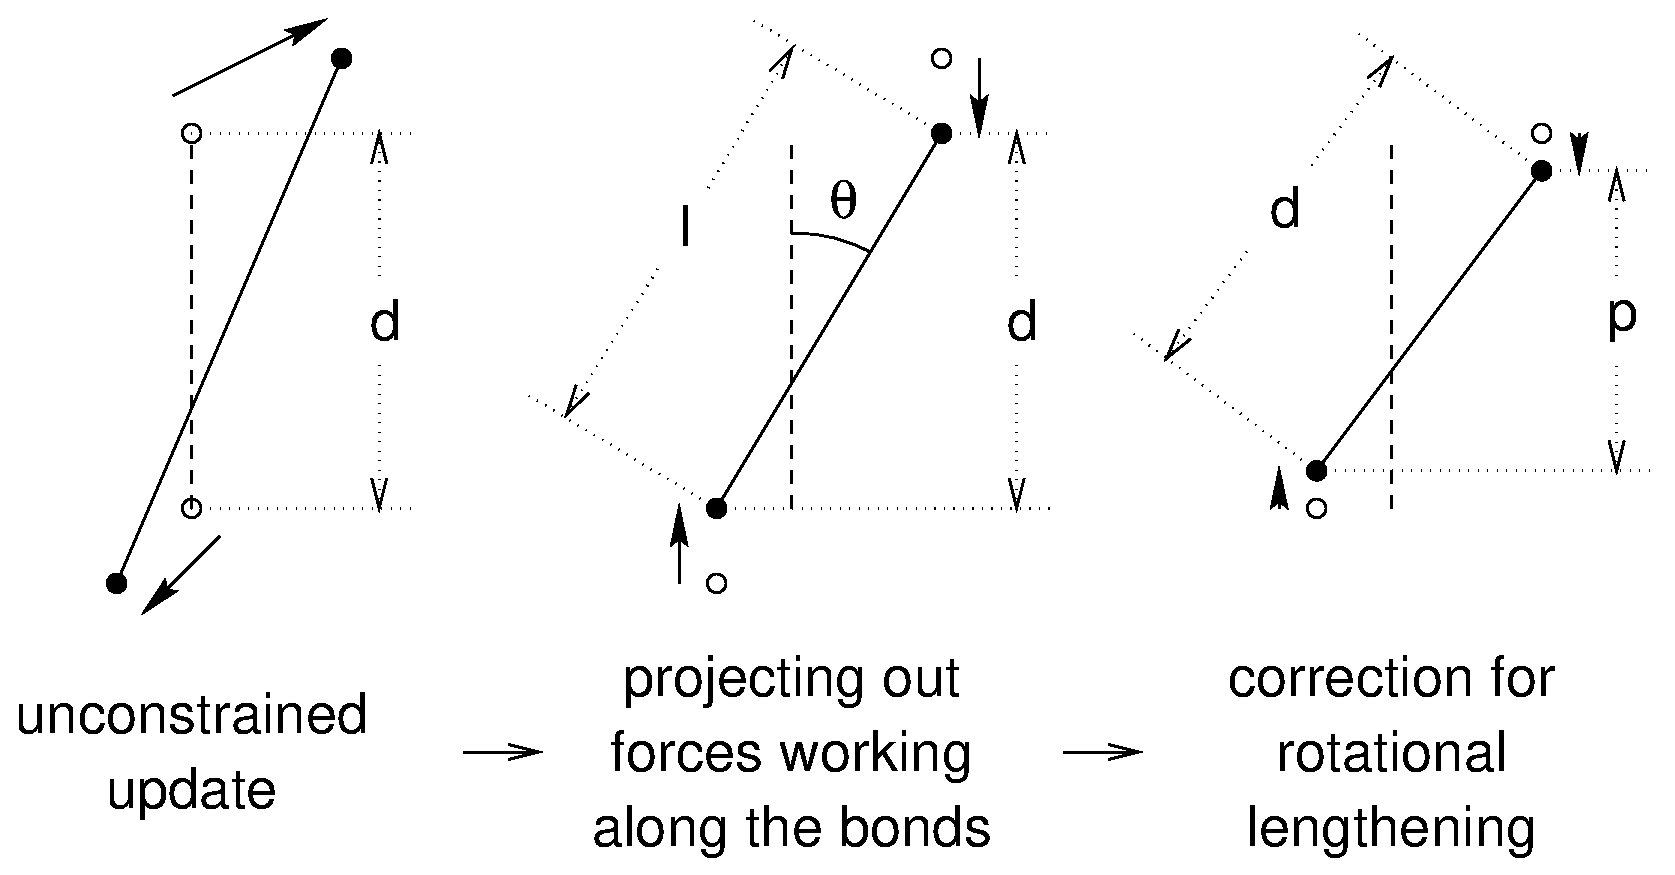
\includegraphics[height=50mm]{plots/lincs}}
\caption[The three position updates needed for one time step.]{The
three position updates needed for one time step. The dashed line is
the old bond of length $d$, the solid lines are the new bonds. $l=d
\cos \theta$ and $p=(2 d^2 - l^2)^{1 \over 2}$.}
\label{fig:lincs}
\end{figure}

A new notation is introduced for the gradient matrix of the constraint 
equations which appears on the right hand side of this equation:
\fs{c3}
B_{hi} = {\p g_h \over \p r_i}
\fe
Notice that $\Bm$ is a $K \times 3N$ matrix, it contains the directions
of the constraints.
The following equation shows how the new constrained coordinates 
$\ve{r}_{n+1}$ are related to the unconstrained coordinates
$\ve{r}_{n+1}^{unc}$ by
\fs{m0}
\begin{array}{c}
  \ve{r}_{n+1}=(\ve{I}-\Tm_n \ve{B}_n) \ve{r}_{n+1}^{unc} + \Tm_n \lenc=  
  \\[2mm]
  \ve{r}_{n+1}^{unc} - 
\iM \Bm_n (\Bm_n \iM \Bm_n^T)^{-1} (\Bm_n \ve{r}_{n+1}^{unc} - \lenc) 
\end{array}
\fe
where $\Tm = \iM \Bm^T (\Bm \iM \Bm^T)^{-1}$.
The derivation of this equation from \eqnsref{c1}{c2} can be found
in \cite{Hess97}.

This first step does not set the real bond lengths to the prescribed lengths,
but the projection of the new bonds onto the old directions of the bonds.
To correct for the rotation of bond $i$, the projection of the
bond, $p_i$, on the old direction is set to
\fs{m1a}
p_i=\sqrt{2 d_i^2 - l_i^2},
\fe
where $l_i$ is the bond length after the first projection.
The corrected positions are
\fs{m1b}
\ve{r}_{n+1}^*=(\ve{I}-\Tm_n \Bm_n)\ve{r}_{n+1} + \Tm_n \ve{p}.
\fe
This correction for rotational effects is actually an iterative process,
but during MD only one iteration is applied.
The relative constraint deviation after this procedure will be less than
0.0001 for every constraint.
In energy minimization, this might not be accurate enough, so the number
of iterations is equal to the order of the expansion (see below).

Half of the CPU time goes to inverting the constraint coupling 
matrix $\Bm_n \iM \Bm_n^T$, which has to be done every time step.
This $K \times K$ matrix
has $1/m_{i_1} + 1/m_{i_2}$ on the diagonal.
The off-diagonal elements are only non-zero when two bonds are connected,
then the element is 
$\cos \phi /m_c$,  where $m_c$ is 
the mass of the atom connecting the
two bonds and $\phi$ is the angle between the bonds.

The matrix $\Tm$ is inverted through a power expansion.
A $K \times K$ matrix $\ve{S}$ is 
introduced which is the inverse square root of 
the diagonal of $\Bm_n \iM \Bm_n^T$.
This matrix is used to convert the diagonal elements 
of the coupling matrix to one:
\fs{m2}
\begin{array}{c}
(\Bm_n \iM \Bm_n^T)^{-1}
= \Sm \Sm^{-1} (\Bm_n \iM \Bm_n^T)^{-1} \Sm^{-1} \Sm  \\[2mm]
= \Sm (\Sm \Bm_n \iM \Bm_n^T \Sm)^{-1} \Sm =
  \Sm (\ve{I} - \ve{A}_n)^{-1} \Sm
\end{array}
\fe
The matrix $\ve{A}_n$ is symmetric and sparse and has zeros on the diagonal.
Thus a simple trick can be used to calculate the inverse:
\fs{m3}
(\ve{I}-\ve{A}_n)^{-1}= 
        \ve{I} + \ve{A}_n + \ve{A}_n^2 + \ve{A}_n^3 + \ldots
\fe

This inversion method is only valid if the absolute values of all the
eigenvalues of $\ve{A}_n$ are smaller than one.
In molecules with only bond constraints, the connectivity is so low
that this will always be true, even if ring structures are present.
Problems can arise in angle-constrained molecules.
By constraining angles with additional distance constraints,
multiple small ring structures are introduced.
This gives a high connectivity, leading to large eigenvalues.
Therefore LINCS should NOT be used with coupled angle-constraints.

For molecules with all bonds constrained the eigenvalues of $A$
are around 0.4. This means that with each additional order
in the expansion \eqnref{m3} the deviations decrease by a factor 0.4.
But for relatively isolated triangles of constraints the largest
eigenvalue is around 0.7.
Such triangles can occur when removing hydrogen angle vibrations
with an additional angle constraint in alcohol groups
or when constraining water molecules with LINCS, for instance
with flexible constraints.
The constraints in such triangles converge twice as slow as
the other constraints. Therefore, starting with {\gromacs} 4,
additional terms are added to the expansion for such triangles
\fs{m3_ang}
(\ve{I}-\ve{A}_n)^{-1} \approx
        \ve{I} + \ve{A}_n + \ldots + \ve{A}_n^{N_i} +
        \left(\ve{A}^*_n + \ldots + {\ve{A}_n^*}^{N_i} \right) \ve{A}_n^{N_i}
\fe
where $N_i$ is the normal order of the expansion and
$\ve{A}^*$ only contains the elements of $\ve{A}$ that couple
constraints within rigid triangles, all other elements are zero.
In this manner, the accuracy of angle constraints comes close
to that of the other constraints, while the series of matrix vector
multiplications required for determining the expansion
only needs to be extended for a few constraint couplings.
This procedure is described in the P-LINCS paper\cite{Hess2008a}.

\subsubsection{The LINCS Parameters}
The accuracy of LINCS depends on the number of matrices used
in the expansion \eqnref{m3}. For MD calculations a fourth order
expansion is enough. For Brownian dynamics with
large time steps an eighth order expansion may be necessary.
The order is a parameter in the {\tt *.mdp} file.
The implementation of LINCS is done in such a way that the 
algorithm will never crash. Even when it is impossible to
to reset the constraints LINCS will generate a conformation
which fulfills the constraints as well as possible.
However, LINCS will generate a warning when in one step a bond 
rotates over more than a predefined angle.
This angle is set by the user in the {\tt *.mdp} file.

% } % Brace matches ifthenelse test for gmxlite


\section{Simulated Annealing}
\label{sec:SA}
The well known \swapindex{simulated}{annealing}
(SA) protocol is supported in {\gromacs}, and you can even couple multiple
groups of atoms separately with an arbitrary number of reference temperatures
that change during the simulation. The annealing is implemented by simply 
changing the current reference temperature for each group in the temperature
coupling, so the actual relaxation and coupling properties depends on the
type of thermostat you use and how hard you are coupling it. Since we are
changing the reference temperature it is important to remember that the system
will NOT instantaneously reach this value - you need to allow for the inherent
relaxation time in the coupling algorithm too. If you are changing the 
annealing reference temperature faster than the temperature relaxation you
will probably end up with a crash when the difference becomes too large.

The annealing protocol is specified as a series of corresponding times and 
reference temperatures for each group, and you can also choose whether you only
want a single sequence (after which the temperature will be coupled to the 
last reference value), or if the annealing should be periodic and restart at 
the first reference point once the sequence is completed. You can mix and
match both types of annealing and non-annealed groups in your simulation.

\newcommand{\vrond}{\stackrel{\circ}{\ve{r}}}
\newcommand{\rond}{\stackrel{\circ}{r}}
\newcommand{\ruis}{\ve{r}^G}

% \ifthenelse{\equal{\gmxlite}{1}}{}{
\section{Stochastic Dynamics\swapindexquiet{stochastic}{dynamics}}
\label{sec:SD}
Stochastic or velocity \swapindex{Langevin}{dynamics} adds a friction
and a noise term to Newton's equations of motion, as
\beq
\label{SDeq}
m_i {\de^2 \ve{r}_i \over \de t^2} =
- m_i \gamma_i {\de \ve{r}_i \over \de t} + \ve{F}_i(\ve{r}) + \vrond_i,
\eeq 
where $\gamma_i$ is the friction constant $[1/\mbox{ps}]$ and
$\vrond_i\!\!(t)$  is a noise process with 
$\langle \rond_i\!\!(t) \rond_j\!\!(t+s) \rangle = 
    2 m_i \gamma_i k_B T \delta(s) \delta_{ij}$.
When $1/\gamma_i$ is large compared to the time scales present in the system,
one could see stochastic dynamics as molecular dynamics with stochastic
temperature-coupling. The advantage compared to MD with Berendsen
temperature-coupling is that in case of SD the generated ensemble is known.
For simulating a system in vacuum there is the additional advantage that there is no
accumulation of errors for the overall translational and rotational
degrees of freedom.
When $1/\gamma_i$ is small compared to the time scales present in the system,
the dynamics will be completely different from MD, but the sampling is
still correct.

In {\gromacs} there is one simple and efficient implementation. Its
accuracy is equivalent to the normal MD leap-frog and
Velocity Verlet integrator. It is nearly identical to the common way of discretizing the Langevin equation, but the friction and velocity term are applied in an impulse fashion~\cite{Goga2012}.
It can be described as:
\bea
\label{eqn:sd_int1}
\ve{v}'  &~=~&   \ve{v}(t-\hDt) + \frac{1}{m}\ve{F}(t)\Dt \\
\Delta\ve{v}     &~=~&   -\alpha \, \ve{v}'(t+\hDt) + \sqrt{\frac{k_B T}{m}(1 - \alpha^2)} \, \ruis_i \\
\ve{r}(t+\Dt)   &~=~&   \ve{r}(t)+\left(\ve{v}' +\frac{1}{2}\Delta \ve{v}\right)\Dt \label{eqn:sd1_x_upd}\\
\ve{v}(t+\hDt)  &~=~&   \ve{v}' + \Delta \ve{v} \\
\alpha &~=~& 1 - e^{-\gamma \Dt}
\eea
where $\ruis_i$ is Gaussian distributed noise with $\mu = 0$, $\sigma = 1$.
The velocity is first updated a full time step without friction and noise to get $\ve{v}'$, identical to the normal update in leap-frog. The friction and noise are then applied as an impulse at step $t+\Dt$. The advantage of this scheme is that the velocity-dependent terms act at the full time step, which makes the correct integration of forces that depend on both coordinates and velocities, such as constraints and dissipative particle dynamics (DPD, not implented yet), straightforward. With constraints, the coordinate update \eqnref{sd1_x_upd} is split into a normal leap-frog update and a $\Delta \ve{v}$. After both of these updates the constraints are applied to coordinates and velocities.

When using SD as a thermostat, an appropriate value for $\gamma$ is e.g. 0.5 ps$^{-1}$,
since this results in a friction that is lower than the internal friction
of water, while it still provides efficient thermostatting.


\section{Brownian Dynamics\swapindexquiet{Brownian}{dynamics}}
\label{sec:BD}
In the limit of high friction, stochastic dynamics reduces to 
Brownian dynamics, also called position Langevin dynamics.
This applies to over-damped systems, 
{\ie} systems in which the inertia effects are negligible.
The equation is
\beq
{\de \ve{r}_i \over \de t} = \frac{1}{\gamma_i} \ve{F}_i(\ve{r}) + \vrond_i
\eeq 
where $\gamma_i$ is the friction coefficient $[\mbox{amu/ps}]$ and
$\vrond_i\!\!(t)$  is a noise process with 
$\langle \rond_i\!\!(t) \rond_j\!\!(t+s) \rangle = 
    2 \delta(s) \delta_{ij} k_B T / \gamma_i$.
In {\gromacs} the equations are integrated with a simple, explicit scheme
\beq
\ve{r}_i(t+\Delta t) = \ve{r}_i(t) +
        {\Delta t \over \gamma_i} \ve{F}_i(\ve{r}(t)) 
        + \sqrt{2 k_B T {\Delta t \over \gamma_i}}\, \ruis_i,
\eeq
where $\ruis_i$ is Gaussian distributed noise with $\mu = 0$, $\sigma = 1$.
The friction coefficients $\gamma_i$ can be chosen the same for all
particles or as $\gamma_i = m_i\,\gamma_i$, where the friction constants
$\gamma_i$ can be different for different groups of atoms. 
Because the system is assumed to be over-damped, large timesteps
can be used. LINCS should be used for the constraints since SHAKE
will not converge for large atomic displacements.
BD is an option of the {\tt mdrun} program.
% } % Brace matches ifthenelse test for gmxlite

\section{Energy Minimization}
\label{sec:EM}\index{energy minimization}%
Energy minimization in {\gromacs} can be done using steepest descent,
conjugate gradients, or l-bfgs (limited-memory
Broyden-Fletcher-Goldfarb-Shanno quasi-Newtonian minimizer...we
prefer the abbreviation). EM is just an option of the {\tt mdrun}
program.

\subsection{Steepest Descent\index{steepest descent}}
Although steepest descent is certainly not the most efficient
algorithm for searching, it is robust and easy to implement.

We define the vector $\ve{r}$ as the vector of all $3N$ coordinates.
Initially a maximum displacement $h_0$ ({\eg} 0.01 nm) must be given. 

First the forces $\ve{F}$ and potential energy are calculated.
New positions are calculated by
\beq
\ve{r}_{n+1} =  \ve{r}_n + \frac{\ve{F}_n}{\max (|\ve{F}_n|)} h_n,
\eeq
where $h_n$ is the maximum displacement and $\ve{F}_n$ is the force,
or the negative gradient of the  potential $V$. The notation $\max
(|\ve{F}_n|)$ means the largest of the absolute values of the force
components.  The forces and energy are again computed for the new positions \\
If ($V_{n+1} < V_n$) the new positions are accepted and $h_{n+1} = 1.2
h_n$. \\
If ($V_{n+1} \geq V_n$) the new positions are rejected and $h_n = 0.2 h_n$.

The algorithm stops when either a user-specified number of force 
evaluations has been performed ({\eg} 100), or when the maximum of the absolute
values of the force (gradient) components is smaller than a specified
value $\epsilon$.
Since force truncation produces some noise in the
energy evaluation, the stopping criterion should not be made too tight
to avoid endless iterations. A reasonable value for $\epsilon$ can be
estimated from the root mean square force $f$ a harmonic oscillator would exhibit at a
temperature $T$. This value is
\beq
  f = 2 \pi \nu \sqrt{ 2mkT},
\eeq
where $\nu$ is the oscillator frequency, $m$ the (reduced) mass, and
$k$ Boltzmann's constant. For a weak oscillator with a wave number of
100 cm$^{-1}$ and a mass of 10 atomic units, at a temperature of 1 K,
$f=7.7$ kJ~mol$^{-1}$~nm$^{-1}$. A value for $\epsilon$ between 1 and
10 is acceptable.   

% \ifthenelse{\equal{\gmxlite}{1}}{}{
\subsection{Conjugate Gradient\index{conjugate gradient}}
Conjugate gradient is slower than steepest descent in the early stages
of the minimization, but becomes more efficient closer to the energy
minimum.  The parameters and stop criterion are the same as for
steepest descent.  In {\gromacs} conjugate gradient can not be used
with constraints, including the SETTLE algorithm for
water~\cite{Miyamoto92}, as this has not been implemented. If water is
present it must be of a flexible model, which can be specified in the
{\tt *.mdp} file by {\tt define = -DFLEXIBLE}.

This is not really a restriction, since the accuracy of conjugate
gradient is only required for minimization prior to a normal-mode
analysis, which cannot be performed with constraints.  For most other
purposes steepest descent is efficient enough.
% } % Brace matches ifthenelse test for gmxlite

% \ifthenelse{\equal{\gmxlite}{1}}{}{
\subsection{\normindex{L-BFGS}}
The original BFGS algorithm works by successively creating better
approximations of the inverse Hessian matrix, and moving the system to
the currently estimated minimum. The memory requirements for this are
proportional to the square of the number of particles, so it is not
practical for large systems like biomolecules. Instead, we use the
L-BFGS algorithm of Nocedal~\cite{Byrd95a,Zhu97a}, which approximates
the inverse Hessian by a fixed number of corrections from previous
steps. This sliding-window technique is almost as efficient as the
original method, but the memory requirements are much lower -
proportional to the number of particles multiplied with the correction
steps. In practice we have found it to converge faster than conjugate
gradients, but due to the correction steps it is not yet parallelized.
It is also noteworthy that switched or shifted interactions usually
improve the convergence, since sharp cut-offs mean the potential
function at the current coordinates is slightly different from the
previous steps used to build the inverse Hessian approximation.
% } % Brace matches ifthenelse test for gmxlite

% \ifthenelse{\equal{\gmxlite}{1}}{}{
\section{Normal-Mode Analysis\index{normal-mode analysis}\index{NMA}}
Normal-mode analysis~\cite{Levitt83,Go83,BBrooks83b} 
can be performed using {\gromacs}, by diagonalization of the mass-weighted
\normindex{Hessian} $H$:
\bea
R^T M^{-1/2} H M^{-1/2} R   &=& \mbox{diag}(\lambda_1,\ldots,\lambda_{3N})
\\
\lambda_i &=& (2 \pi \omega_i)^2
\eea
where $M$ contains the atomic masses, $R$ is a matrix that contains
the eigenvectors as columns, $\lambda_i$ are the eigenvalues
and $\omega_i$ are the corresponding frequencies.

First the Hessian matrix, which is a $3N \times 3N$ matrix where $N$
is the number of atoms, needs to be calculated:
\bea
H_{ij}  &=&     \frac{\partial^2 V}{\partial x_i \partial x_j}
\eea
where $x_i$ and $x_j$ denote the atomic x, y or z coordinates.
In practice, this equation is not used, but the Hessian is
calculated numerically from the force as:
\bea
H_{ij} &=& -
  \frac{f_i({\bf x}+h{\bf e}_j) - f_i({\bf x}-h{\bf e}_j)}{2h}
\\
f_i     &=& - \frac{\partial V}{\partial x_i}
\eea
where ${\bf e}_j$ is the unit vector in direction $j$.
It should be noted that
for a usual normal-mode calculation, it is necessary to completely minimize 
the energy prior to computation of the Hessian.
The tolerance required depends on the type of system,
but a rough indication is 0.001 kJ mol$^{-1}$.
Minimization should be done with conjugate gradients or L-BFGS in double precision.

A number of {\gromacs} programs are involved in these
calculations. First, the energy should be minimized using {\tt mdrun}.
Then, {\tt mdrun} computes the Hessian.  {\bf Note} that for generating
the run input file, one should use the minimized conformation from
the full precision trajectory file, as the structure file is not
accurate enough.
{\tt \normindex{gmx nmeig}} does the diagonalization and
the sorting of the normal modes according to their frequencies.
Both {\tt mdrun} and {\tt gmx nmeig} should be run in double precision.
The normal modes can be analyzed with the program {\tt gmx anaeig}.
Ensembles of structures at any temperature and for any subset of
normal modes can be generated with {\tt \normindex{gmx nmens}}.
An overview of normal-mode analysis and the related principal component
analysis (see \secref{covanal}) can be found in~\cite{Hayward95b}.
% } % Brace matches ifthenelse test for gmxlite

% \ifthenelse{\equal{\gmxlite}{1}}{}{

\section{Free energy calculations\index{free energy calculations}}
\label{sec:fecalc}
\subsection{Slow-growth methods\index{slow-growth methods}}
Free energy calculations can be performed
in {\gromacs} using  a number of methods, including ``slow-growth.'' An example problem 
might be calculating the difference in free energy of binding of an inhibitor {\bf I}
to an enzyme {\bf E} and to a mutated enzyme {\bf E$^{\prime}$}. It 
is not feasible with computer simulations to perform a docking
calculation for such a large complex, or even releasing the inhibitor from
the enzyme in a reasonable amount of computer time with reasonable accuracy.
However, if we consider the free energy cycle in~\figref{free}A
we can write:
\beq
\Delta G_1 - \Delta G_2 =       \Delta G_3 - \Delta G_4
\label{eqn:ddg}
\eeq
If we are interested in the left-hand term we can equally well compute
the right-hand term.
\begin{figure}
\centerline{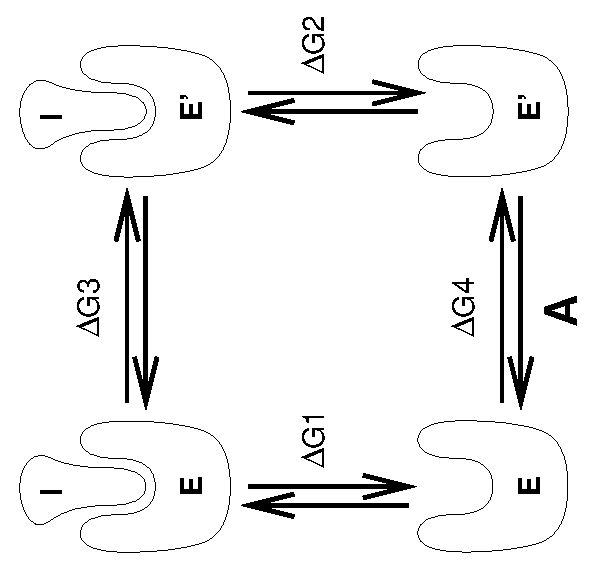
\includegraphics[width=6cm,angle=270]{plots/free1}\hspace{2cm}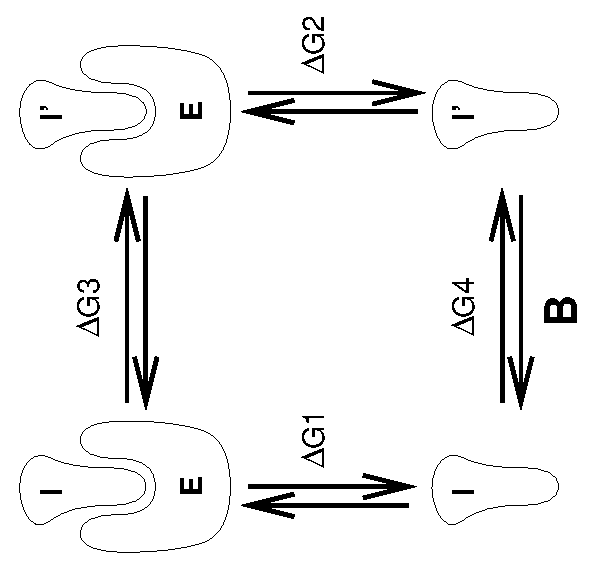
\includegraphics[width=6cm,angle=270]{plots/free2}}
\caption[Free energy cycles.]{Free energy cycles. {\bf A:} to
calculate $\Delta G_{12}$, the free energy difference between the
binding of inhibitor {\bf I} to enzymes {\bf E} respectively {\bf
E$^{\prime}$}. {\bf B:} to calculate $\Delta G_{12}$, the free energy
difference for binding of inhibitors {\bf I} respectively {\bf I$^{\prime}$} to
enzyme {\bf E}.}
\label{fig:free}
\end{figure}

If we want to compute the difference in free energy of binding of two
inhibitors {\bf I} and {\bf I$^{\prime}$} to an enzyme {\bf E} (\figref{free}B)
we can again use \eqnref{ddg} to compute the desired property.

\newcommand{\sA}{^{\mathrm{A}}}
\newcommand{\sB}{^{\mathrm{B}}}
Free energy differences between two molecular species can
be calculated in {\gromacs} using the ``slow-growth'' method.
Such free energy differences between different molecular species are
physically meaningless, but they can be used to obtain meaningful
quantities employing a thermodynamic cycle.
The method requires a simulation during which the Hamiltonian of the
system changes slowly from that describing one system (A) to that
describing the other system (B). The change must be so slow that the
system remains in equilibrium during the process; if that requirement
is fulfilled, the change is reversible and a slow-growth simulation from B to A
will yield the same results (but with a different sign) as a slow-growth
simulation from A to B. This is a useful check, but the user should be
aware of the danger that equality of forward and backward growth results does
not guarantee correctness of the results.

The required modification of the Hamiltonian $H$ is realized by making
$H$ a function of a \textit{coupling parameter} $\lambda:
H=H(p,q;\lambda)$ in such a way that $\lambda=0$ describes system A
and $\lambda=1$ describes system B: 
\beq
  H(p,q;0)=H\sA (p,q);~~~~ H(p,q;1)=H\sB (p,q).
\eeq
In {\gromacs}, the functional form of the $\lambda$-dependence is
different for the various force-field contributions and is described
in section \secref{feia}.

The Helmholtz free energy $A$ is related to the
partition function $Q$ of an $N,V,T$ ensemble, which is assumed to be
the equilibrium ensemble generated by a MD simulation at constant
volume and temperature. The generally more useful Gibbs free energy
$G$ is related to the partition function $\Delta$ of an $N,p,T$
ensemble, which is assumed to be the equilibrium ensemble generated by
a MD simulation at constant pressure and temperature:
\bea
 A(\lambda) &=&  -k_BT \ln Q \\
 Q &=& c \int\!\!\int \exp[-\beta H(p,q;\lambda)]\,dp\,dq \\
 G(\lambda) &=&  -k_BT \ln \Delta \\
 \Delta &=& c \int\!\!\int\!\!\int \exp[-\beta H(p,q;\lambda) -\beta
pV]\,dp\,dq\,dV \\
G &=& A + pV, 
\eea
where $\beta = 1/(k_BT)$ and $c = (N! h^{3N})^{-1}$.
These integrals over phase space cannot be evaluated from a
simulation, but it is possible to evaluate the derivative with 
respect to $\lambda$ as an ensemble average:
\beq
 \frac{dA}{d\lambda} =  \frac{\int\!\!\int (\partial H/ \partial
\lambda) \exp[-\beta H(p,q;\lambda)]\,dp\,dq}{\int\!\!\int \exp[-\beta
H(p,q;\lambda)]\,dp\,dq} = 
\left\langle \frac{\partial H}{\partial \lambda} \right\rangle_{NVT;\lambda},
\eeq
with a similar relation for $dG/d\lambda$ in the $N,p,T$
ensemble.  The difference in free energy between A and B can be found
by integrating the derivative over $\lambda$:
\bea
  A\sB(V,T)-A\sA(V,T) &=& \int_0^1 \left\langle \frac{\partial
H}{\partial \lambda} \right\rangle_{NVT;\lambda} \,d\lambda 
\label{eq:delA} \\
 G\sB(p,T)-G\sA(p,T) &=& \int_0^1 \left\langle \frac{\partial
H}{\partial \lambda} \right\rangle_{NpT;\lambda} \,d\lambda.
\label{eq:delG}
\eea
If one wishes to evaluate $G\sB(p,T)-G\sA(p,T)$,
the natural choice is a constant-pressure simulation. However, this
quantity can also be obtained from a slow-growth simulation at
constant volume, starting with system A at pressure $p$ and volume $V$
and ending with system B at pressure $p_B$, by applying the following
small (but, in principle, exact) correction: 
\beq
  G\sB(p)-G\sA(p) =
A\sB(V)-A\sA(V) - \int_p^{p\sB}[V\sB(p')-V]\,dp'
\eeq
Here we omitted the constant $T$ from the notation. This correction is
roughly equal to $-\frac{1}{2} (p\sB-p)\Delta V=(\Delta V)^2/(2
\kappa V)$, where $\Delta V$ is the volume change at $p$ and $\kappa$
is the isothermal compressibility. This is usually
small; for example, the growth of a water molecule from nothing
in a bath of 1000 water molecules at constant volume would produce an
additional pressure of as much as 22 bar, but a correction to the 
Helmholtz free energy of just -1 kJ mol$^{-1}$. %-20 J/mol.

In Cartesian coordinates, the kinetic energy term in the Hamiltonian
depends only on the momenta, and can be separately integrated and, in
fact, removed from the equations. When masses do not change, there is
no contribution from the kinetic energy at all; otherwise the
integrated contribution to the free energy is $-\frac{3}{2} k_BT \ln
(m\sB/m\sA)$. {\bf Note} that this is only true in the absence of constraints.

\subsection{Thermodynamic integration\index{thermodynamic integration}\index{BAR}\index{Bennett's acceptance ratio}}  
{\gromacs} offers the possibility to integrate eq.~\ref{eq:delA} or
eq. \ref{eq:delG} in one simulation over the full range from A to
B. However, if the change is large and insufficient sampling can be
expected, the user may prefer to determine the value of $\langle
dG/d\lambda \rangle$ accurately at a number of well-chosen
intermediate values of $\lambda$. This can easily be done by setting
the stepsize {\tt delta_lambda} to zero. Each simulation can be
equilibrated first, and a proper error estimate can be made for each
value of $dG/d\lambda$ from the fluctuation of $\partial H/\partial
\lambda$. The total free energy change is then determined afterward
by an appropriate numerical integration procedure.

{\gromacs} now also supports the use of Bennett's Acceptance Ratio~\cite{Bennett1976}
for calculating values of $\Delta$G for transformations from state A to state B using
the program {\tt \normindex{gmx bar}}. The same data can also be used to calculate free
energies using MBAR~\cite{Shirts2008}, though the analysis currently requires external tools from
the external {\tt pymbar} package, at https://SimTK.org/home/pymbar.

The $\lambda$-dependence for the force-field contributions is
described in detail in section \secref{feia}.
% } % Brace matches ifthenelse test for gmxlite

% \ifthenelse{\equal{\gmxlite}{1}}{}{
\section{Replica exchange\index{replica exchange}}
Replica exchange molecular dynamics (\normindex{REMD})
is a method that can be used to speed up
the sampling of any type of simulation, especially if
conformations are separated by relatively high energy barriers.
It involves simulating multiple replicas of the same system
at different temperatures and randomly exchanging the complete state
of two replicas at regular intervals with the probability:
\beq
P(1 \leftrightarrow 2)=\min\left(1,\exp\left[
\left(\frac{1}{k_B T_1} - \frac{1}{k_B T_2}\right)(U_1 - U_2)
 \right] \right)
\eeq
where $T_1$ and $T_2$ are the reference temperatures and $U_1$ and $U_2$
are the instantaneous potential energies of replicas 1 and 2 respectively.
After exchange the velocities are scaled by $(T_1/T_2)^{\pm0.5}$
and a neighbor search is performed the next step.
This combines the fast sampling and frequent barrier-crossing
of the highest temperature with correct Boltzmann sampling at
all the different temperatures~\cite{Hukushima96a,Sugita99}.
We only attempt exchanges for neighboring temperatures as the probability
decreases very rapidly with the temperature difference.
One should not attempt exchanges for all possible pairs in one step.
If, for instance, replicas 1 and 2 would exchange, the chance of
exchange for replicas 2 and 3 not only depends on the energies of
replicas 2 and 3, but also on the energy of replica 1.
In {\gromacs} this is solved by attempting exchange for all ``odd''
pairs on ``odd'' attempts and for all ``even'' pairs on ``even'' attempts.
If we have four replicas: 0, 1, 2 and 3, ordered in temperature
and we attempt exchange every 1000 steps, pairs 0-1 and 2-3
will be tried at steps 1000, 3000 etc. and pair 1-2 at steps 2000, 4000 etc.

How should one choose the temperatures?
The energy difference can be written as:
\beq
U_1 - U_2 =  N_{df} \frac{c}{2} k_B (T_1 - T_2)
\eeq
where $N_{df}$ is the total number of degrees of freedom of one replica
and $c$ is 1 for harmonic potentials and around 2 for protein/water systems.
If $T_2 = (1+\epsilon) T_1$ the probability becomes:
\beq
P(1 \leftrightarrow 2)
  = \exp\left( -\frac{\epsilon^2 c\,N_{df}}{2 (1+\epsilon)} \right)
\approx \exp\left(-\epsilon^2 \frac{c}{2} N_{df} \right)
\eeq
Thus for a probability of $e^{-2}\approx 0.135$
one obtains $\epsilon \approx 2/\sqrt{c\,N_{df}}$.
With all bonds constrained one has $N_{df} \approx 2\, N_{atoms}$
and thus for $c$ = 2 one should choose $\epsilon$ as $1/\sqrt{N_{atoms}}$.
However there is one problem when using pressure coupling. The density at
higher temperatures will decrease, leading to higher energy~\cite{Seibert2005a},
which should be taken into account. The {\gromacs} website features a
so-called ``REMD calculator,'' that lets you type in the temperature range and
the number of atoms, and based on that proposes a set of temperatures.

An extension to the REMD for the isobaric-isothermal ensemble was
proposed by Okabe {\em et al.}~\cite{Okabe2001a}. In this work the
exchange probability is modified to:
\beq
P(1 \leftrightarrow 2)=\min\left(1,\exp\left[
\left(\frac{1}{k_B T_1} - \frac{1}{k_B T_2}\right)(U_1 - U_2) +
\left(\frac{P_1}{k_B T_1} - \frac{P_2}{k_B T_2}\right)\left(V_1-V_2\right)
 \right] \right)
\eeq
where $P_1$ and $P_2$ are the respective reference pressures and $V_1$ and
$V_2$ are the respective instantaneous volumes in the simulations.
In most cases the differences in volume are so small that the second
term is negligible. It only plays a role when the difference between
$P_1$ and $P_2$ is large or in phase transitions.

Hamiltonian replica exchange is also supported in {\gromacs}.  In
Hamiltonian replica exchange, each replica has a different
Hamiltonian, defined by the free energy pathway specified for the simulation.  The
exchange probability to maintain the correct ensemble probabilities is:
\beq P(1 \leftrightarrow 2)=\min\left(1,\exp\left[
    \left(\frac{1}{k_B T} - \frac{1}{k_B T}\right)((U_1(x_2) - U_1(x_1)) + (U_2(x_1) - U_2(x_2)))
\right]
\right)
\eeq
The separate Hamiltonians are defined by the free energy functionality
of {\gromacs}, with swaps made between the different values of
$\lambda$ defined in the mdp file.

Hamiltonian and temperature replica exchange can also be performed
simultaneously, using the acceptance criteria:
\beq
P(1 \leftrightarrow 2)=\min\left(1,\exp\left[
\left(\frac{1}{k_B T} - \right)(\frac{U_1(x_2) - U_1(x_1)}{k_B T_1} + \frac{U_2(x_1) - U_2(x_2)}{k_B T_2})
 \right] \right)
\eeq

Gibbs sampling replica exchange has also been implemented in
{\gromacs}~\cite{Chodera2011}.  In Gibbs sampling replica exchange, all
possible pairs are tested for exchange, allowing swaps between
replicas that are not neighbors.

Gibbs sampling replica exchange requires no additional potential
energy calculations.  However there is an additional communication
cost in Gibbs sampling replica exchange, as for some permutations,
more than one round of swaps must take place.  In some cases, this
extra communication cost might affect the efficiency.

All replica exchange variants are options of the {\tt mdrun}
program. It will only work when MPI is installed, due to the inherent
parallelism in the algorithm. For efficiency each replica can run on a
separate rank.  See the manual page of {\tt mdrun} on how to use these
multinode features.

% \ifthenelse{\equal{\gmxlite}{1}}{}{

\section{Essential Dynamics sampling\index{essential dynamics}\index{principal component analysis}\seeindexquiet{PCA}{covariance analysis}}
The results from Essential Dynamics (see \secref{covanal})
of a protein can be used to guide MD simulations. The idea is that
from an initial MD simulation (or from other sources) a definition of
the collective fluctuations with largest amplitude is obtained. The
position along one or more of these collective modes can be
constrained in a (second) MD simulation in a number of ways for
several purposes. For example, the position along a certain mode may
be kept fixed to monitor the average force (free-energy gradient) on
that coordinate in that position. Another application is to enhance
sampling efficiency with respect to usual MD
\cite{Degroot96a,Degroot96b}. In this case, the system is encouraged
to sample its available configuration space more systematically than
in a diffusion-like path that proteins usually take.

Another possibility to enhance sampling is \normindex{flooding}.
Here a flooding potential is added to certain
(collective) degrees of freedom to expel the system out
of a region of phase space \cite{Lange2006a}.

The procedure for essential dynamics sampling or flooding is as follows.
First, the eigenvectors and eigenvalues need to be determined
using covariance analysis ({\tt gmx covar})
or normal-mode analysis ({\tt gmx nmeig}).
Then, this information is fed into {\tt make_edi},
which has many options for selecting vectors and setting parameters,
see {\tt gmx make_edi -h}.
The generated {\tt edi} input file is then passed to {\tt mdrun}.

% } % Brace matches ifthenelse test for gmxlite

% \ifthenelse{\equal{\gmxlite}{1}}{}{
\section{\normindex{Expanded Ensemble}}

In an expanded ensemble simulation~\cite{Lyubartsev1992}, both the coordinates and the
thermodynamic ensemble are treated as configuration variables that can
be sampled over.  The probability of any given state can be written as:
\beq
P(\vec{x},k) \propto \exp\left(-\beta_k U_k + g_k\right),
\eeq
where $\beta_k = \frac{1}{k_B T_k}$ is the $\beta$ corresponding to the $k$th
thermodynamic state, and $g_k$ is a user-specified weight factor corresponding
to the $k$th state.  This space is therefore a {\em mixed}, {\em generalized}, or {\em
  expanded} ensemble which samples from multiple thermodynamic
ensembles simultaneously. $g_k$ is chosen to give a specific weighting
of each subensemble in the expanded ensemble, and can either be fixed,
or determined by an iterative procedure. The set of $g_k$ is
frequently chosen to give each thermodynamic ensemble equal
probability, in which case $g_k$ is equal to the free energy in
non-dimensional units, but they can be set to arbitrary values as
desired.  Several different algorithms can be used to equilibrate
these weights, described in the mdp option listings.
% } % Brace matches ifthenelse test for gmxlite

In {\gromacs}, this space is sampled by alternating sampling in the $k$
and $\vec{x}$ directions.  Sampling in the $\vec{x}$ direction is done
by standard molecular dynamics sampling; sampling between the
different thermodynamics states is done by Monte Carlo, with several
different Monte Carlo moves supported. The $k$ states can be defined
by different temperatures, or choices of the free energy $\lambda$
variable, or both.  Expanded ensemble simulations thus represent a
serialization of the replica exchange formalism, allowing a single
simulation to explore many thermodynamic states.



\section{Parallelization\index{parallelization}}
The CPU time required for a simulation can be reduced by running the simulation
in parallel over more than one core.
Ideally, one would want to have linear scaling: running on $N$ cores
makes the simulation $N$ times faster. In practice this can only be
achieved for a small number of cores. The scaling will depend
a lot on the algorithms used. Also, different algorithms can have different
restrictions on the interaction ranges between atoms.

\section{Domain decomposition\index{domain decomposition}}
Since most interactions in molecular simulations are local,
domain decomposition is a natural way to decompose the system.
In domain decomposition, a spatial domain is assigned to each rank,
which will then integrate the equations of motion for the particles
that currently reside in its local domain. With domain decomposition,
there are two choices that have to be made: the division of the unit cell
into domains and the assignment of the forces to domains.
Most molecular simulation packages use the half-shell method for assigning
the forces. But there are two methods that always require less communication:
the eighth shell~\cite{Liem1991} and the midpoint~\cite{Shaw2006} method.
{\gromacs} currently uses the eighth shell method, but for certain systems
or hardware architectures it might be advantageous to use the midpoint
method. Therefore, we might implement the midpoint method in the future.
Most of the details of the domain decomposition can be found
in the {\gromacs} 4 paper~\cite{Hess2008b}.

\subsection{Coordinate and force communication}
In the most general case of a triclinic unit cell,
the space in divided with a 1-, 2-, or 3-D grid in parallelepipeds
that we call domain decomposition cells.
Each cell is assigned to a particle-particle rank.
The system is partitioned over the ranks at the beginning
of each MD step in which neighbor searching is performed.
Since the neighbor searching is based on charge groups, charge groups
are also the units for the domain decomposition.
Charge groups are assigned to the cell where their center of geometry resides.
Before the forces can be calculated, the coordinates from some
neighboring cells need to be communicated,
and after the forces are calculated, the forces need to be communicated
in the other direction.
The communication and force assignment is based on zones that 
can cover one or multiple cells.
An example of a zone setup is shown in \figref{ddcells}.

\begin{figure}
\centerline{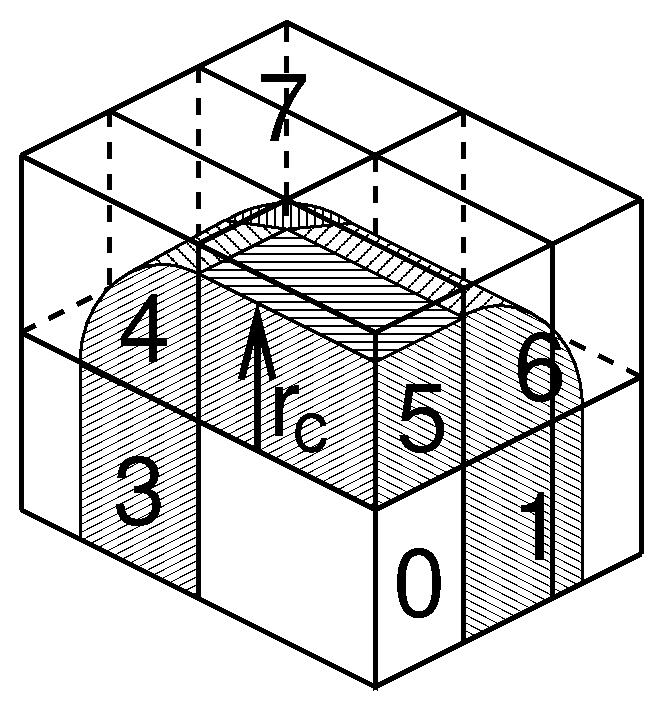
\includegraphics[width=6cm]{plots/dd-cells}}
\caption{
A non-staggered domain decomposition grid of 3$\times$2$\times$2 cells.
Coordinates in zones 1 to 7 are communicated to the corner cell
that has its home particles in zone 0.
$r_c$ is the cut-off radius. 
\label{fig:ddcells}
}
\end{figure}

The coordinates are communicated by moving data along the ``negative''
direction in $x$, $y$ or $z$ to the next neighbor. This can be done in one
or multiple pulses. In \figref{ddcells} two pulses in $x$ are required,
then one in $y$ and then one in $z$. The forces are communicated by
reversing this procedure. See the {\gromacs} 4 paper~\cite{Hess2008b}
for details on determining which non-bonded and bonded forces
should be calculated on which rank.

\subsection{Dynamic load balancing\swapindexquiet{dynamic}{load balancing}}
When different ranks have a different computational load
(load imbalance), all ranks will have to wait for the one
that takes the most time. One would like to avoid such a situation.
Load imbalance can occur due to four reasons:
\begin{itemize}
\item inhomogeneous particle distribution
\item inhomogeneous interaction cost distribution (charged/uncharged,
  water/non-water due to {\gromacs} water innerloops)
\item statistical fluctuation (only with small particle numbers)
\item differences in communication time, due to network topology and/or other jobs on the machine interfering with our communication
\end{itemize}
So we need a dynamic load balancing algorithm
where the volume of each domain decomposition cell
can be adjusted {\em independently}.
To achieve this, the 2- or 3-D domain decomposition grids need to be
staggered. \figref{ddtric} shows the most general case in 2-D.
Due to the staggering, one might require two distance checks
for deciding if a charge group needs to be communicated:
a non-bonded distance and a bonded distance check.

\begin{figure}
\centerline{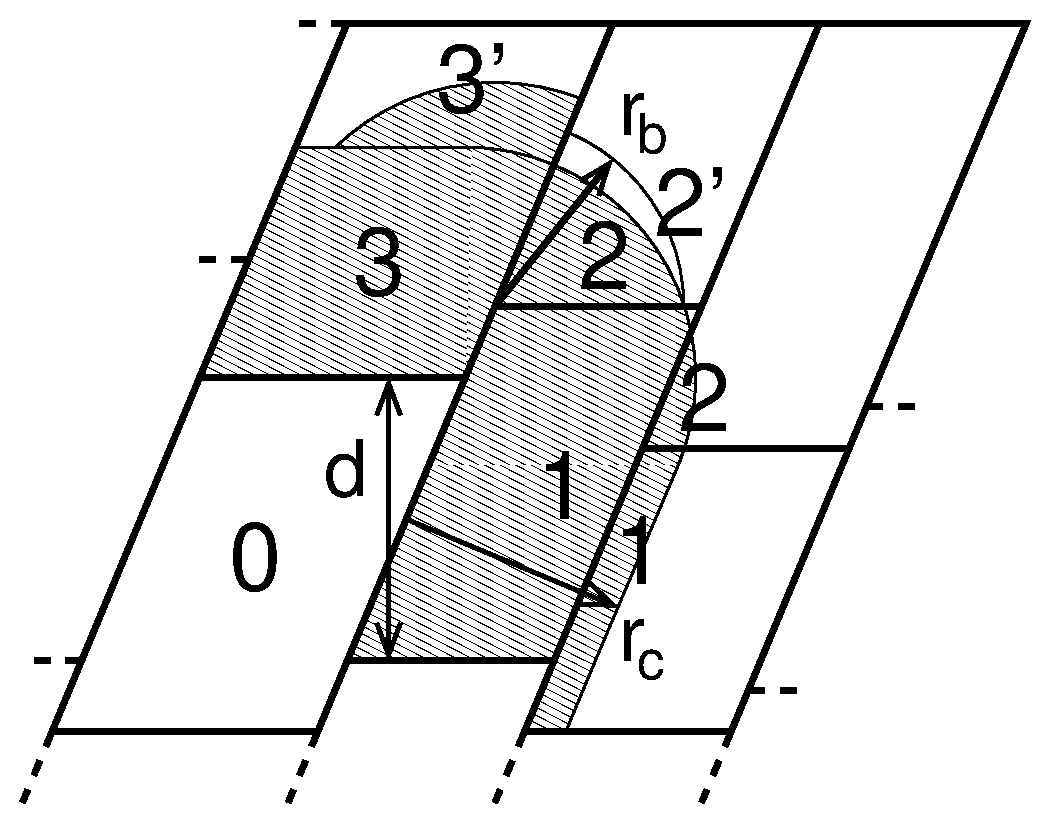
\includegraphics[width=7cm]{plots/dd-tric}}
\caption{
The zones to communicate to the rank of zone 0,
see the text for details. $r_c$ and $r_b$ are the non-bonded
and bonded cut-off radii respectively, $d$ is an example
of a distance between following, staggered boundaries of cells.
\label{fig:ddtric}
}
\end{figure}

By default, {\tt mdrun} automatically turns on the dynamic load
balancing during a simulation when the total performance loss
due to the force calculation imbalance is 2\% or more.
{\bf Note} that the reported force load imbalance numbers might be higher,
since the force calculation is only part of work that needs to be done
during an integration step.
The load imbalance is reported in the log file at log output steps
and when the {\tt -v} option is used also on screen.
The average load imbalance and the total performance loss
due to load imbalance are reported at the end of the log file.

There is one important parameter for the dynamic load balancing,
which is the minimum allowed scaling. By default, each dimension
of the domain decomposition cell can scale down by at least
a factor of 0.8. For 3-D domain decomposition this allows cells
to change their volume by about a factor of 0.5, which should allow
for compensation of a load imbalance of 100\%.
The minimum allowed scaling can be changed with the {\tt -dds}
option of {\tt mdrun}.

The load imbalance is measured by timing a single region of the MD step
on each MPI rank. This region can not include MPI communication, as
timing of MPI calls does not allow separating wait due to imbalance
from actual communication.
The domain volumes are then scaled, with under-relaxation, inversely
proportional with the measured time. This procedure will decrease the
load imbalance when the change in load in the measured region correlates
with the change in domain volume and the load outside
the measured region does not depend strongly on the domain volume.
In CPU-only simulations, the load is measured between the coordinate
and the force communication. In hybrid CPU-GPU simulations we overlap
communication on the CPU with calculation on the GPU. Therefore we
measure from the last communication before the force calculation to
when the CPU or GPU is finished, whichever is last.
When not using PME ranks, we subtract the time in PME from the CPU time,
as this includes MPI calls and the PME load is independent of domain size.
This generally works well, unless the non-bonded load is low and there is
imbalance in the bonded interactions. Then two issues can arise.
Dynamic load balancing can increase the imbalance in update and constraints
and with PME the coordinate and force redistribution time can go up
significantly. Although dynamic load balancing
can significantly improve performance in cases where there is imbalance in
the bonded interactions on the CPU, there are many situations in which
some domains continue decreasing in size and the load imbalance increases
and/or PME coordinate and force redistribution cost increases significantly.
As of version 2016.1, {\tt mdrun} disables the dynamic load balancing when
measurement indicates that it deteriorates performance. This means that in most
cases the user will get good performance with the default, automated
dynamic load balancing setting.

\subsection{Constraints in parallel\index{constraints}}
\label{subsec:plincs}
Since with domain decomposition parts of molecules can reside
on different ranks, bond constraints can cross cell boundaries.
Therefore a parallel constraint algorithm is required.
{\gromacs} uses the \normindex{P-LINCS} algorithm~\cite{Hess2008a},
which is the parallel version of the \normindex{LINCS} algorithm~\cite{Hess97}
% \ifthenelse{\equal{\gmxlite}{1}}
{.}
{(see \ssecref{lincs}).}
The P-LINCS procedure is illustrated in \figref{plincs}.
When molecules cross the cell boundaries, atoms in such molecules
up to ({\tt lincs_order + 1}) bonds away are communicated over the cell boundaries.
Then, the normal LINCS algorithm can be applied to the local bonds
plus the communicated ones. After this procedure, the local bonds
are correctly constrained, even though the extra communicated ones are not.
One coordinate communication step is required for the initial LINCS step
and one for each iteration. Forces do not need to be communicated.

\begin{figure}
\centerline{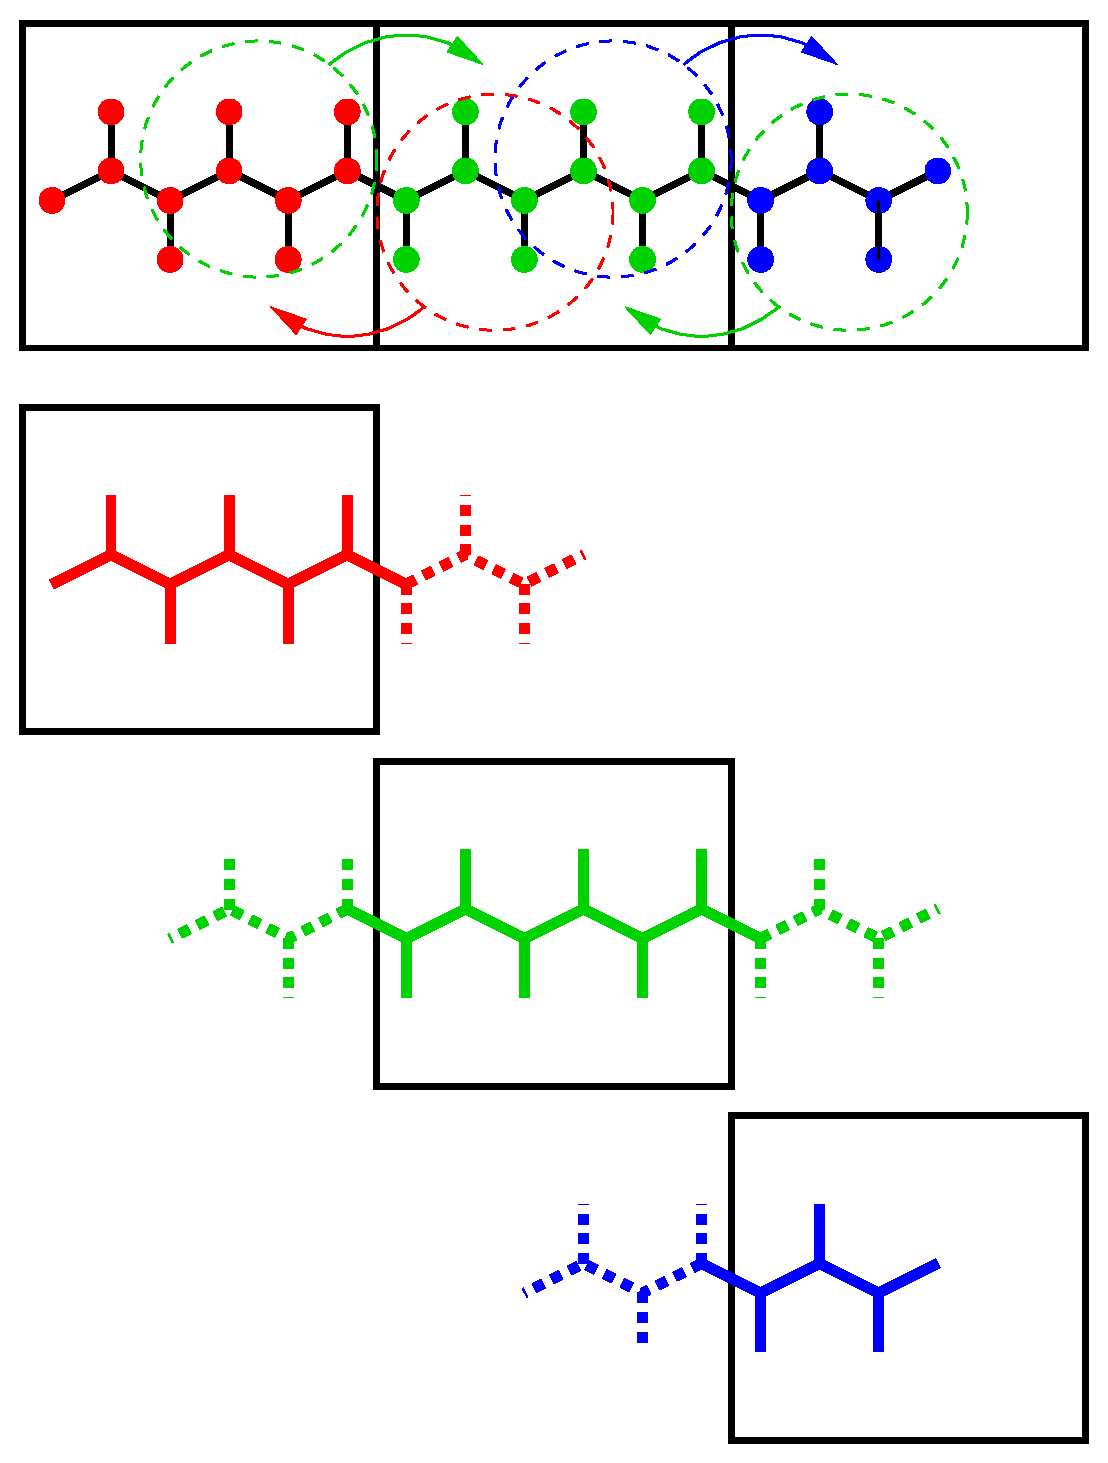
\includegraphics[width=6cm]{plots/par-lincs2}}
\caption{
Example of the parallel setup of P-LINCS with one molecule
split over three domain decomposition cells, using a matrix
expansion order of 3.
The top part shows which atom coordinates need to be communicated
to which cells. The bottom parts show the local constraints (solid)
and the non-local constraints (dashed) for each of the three cells.
\label{fig:plincs}
}
\end{figure}

\subsection{Interaction ranges}
Domain decomposition takes advantage of the locality of interactions.
This means that there will be limitations on the range of interactions.
By default, {\tt mdrun} tries to find the optimal balance between
interaction range and efficiency. But it can happen that a simulation
stops with an error message about missing interactions,
or that a simulation might run slightly faster with shorter
interaction ranges. A list of interaction ranges
and their default values is given in \tabref{dd_ranges}.

\begin{table}
\centerline{
\begin{tabular}{|c|c|ll|}
\dline
interaction & range & option & default \\
\dline
non-bonded        & $r_c$ = max($r_{\mathrm{list}}$,$r_{\mathrm{VdW}}$,$r_{\mathrm{Coul}}$) & {\tt mdp} file & \\
two-body bonded   & max($r_{\mathrm{mb}}$,$r_c$) & {\tt mdrun -rdd} & starting conf. + 10\% \\
multi-body bonded & $r_{\mathrm{mb}}$ & {\tt mdrun -rdd} & starting conf. + 10\% \\
constraints       & $r_{\mathrm{con}}$ & {\tt mdrun -rcon} & est. from bond lengths \\
virtual sites     & $r_{\mathrm{con}}$ & {\tt mdrun -rcon} & 0 \\
\dline
\end{tabular}
}
\caption{The interaction ranges with domain decomposition.}
\label{tab:dd_ranges}
\end{table}

In most cases the defaults of {\tt mdrun} should not cause the simulation
to stop with an error message of missing interactions.
The range for the bonded interactions is determined from the distance
between bonded charge-groups in the starting configuration, with 10\% added
for headroom. For the constraints, the value of $r_{\mathrm{con}}$ is determined by
taking the maximum distance that ({\tt lincs_order + 1}) bonds can cover
when they all connect at angles of 120 degrees.
The actual constraint communication is not limited by $r_{\mathrm{con}}$,
but by the minimum cell size $L_C$, which has the following lower limit:
\beq
L_C \geq \max(r_{\mathrm{mb}},r_{\mathrm{con}})
\eeq
Without dynamic load balancing the system is actually allowed to scale
beyond this limit when pressure scaling is used.
{\bf Note} that for triclinic boxes, $L_C$ is not simply the box diagonal
component divided by the number of cells in that direction,
rather it is the shortest distance between the triclinic cells borders.
For rhombic dodecahedra this is a factor of $\sqrt{3/2}$ shorter
along $x$ and $y$.

When $r_{\mathrm{mb}} > r_c$, {\tt mdrun} employs a smart algorithm to reduce
the communication. Simply communicating all charge groups within
$r_{\mathrm{mb}}$ would increase the amount of communication enormously.
Therefore only charge-groups that are connected by bonded interactions
to charge groups which are not locally present are communicated.
This leads to little extra communication, but also to a slightly
increased cost for the domain decomposition setup.
In some cases, {\eg} coarse-grained simulations with a very short cut-off,
one might want to set $r_{\mathrm{mb}}$ by hand to reduce this cost.

\subsection{Multiple-Program, Multiple-Data PME parallelization\index{PME}}
\label{subsec:mpmd_pme}
Electrostatics interactions are long-range, therefore special
algorithms are used to avoid summation over many atom pairs.
In {\gromacs} this is usually
% \ifthenelse{\equal{\gmxlite}{1}}
{.}
{PME (\secref{pme}).}
Since with PME all particles interact with each other, global communication
is required. This will usually be the limiting factor for 
scaling with domain decomposition.
To reduce the effect of this problem, we have come up with
a Multiple-Program, Multiple-Data approach~\cite{Hess2008b}.
Here, some ranks are selected to do only the PME mesh calculation,
while the other ranks, called particle-particle (PP) ranks,
do all the rest of the work.
For rectangular boxes the optimal PP to PME rank ratio is usually 3:1,
for rhombic dodecahedra usually 2:1.
When the number of PME ranks is reduced by a factor of 4, the number
of communication calls is reduced by about a factor of 16.
Or put differently, we can now scale to 4 times more ranks.
In addition, for modern 4 or 8 core machines in a network,
the effective network bandwidth for PME is quadrupled,
since only a quarter of the cores will be using the network connection
on each machine during the PME calculations.

\begin{figure}
\centerline{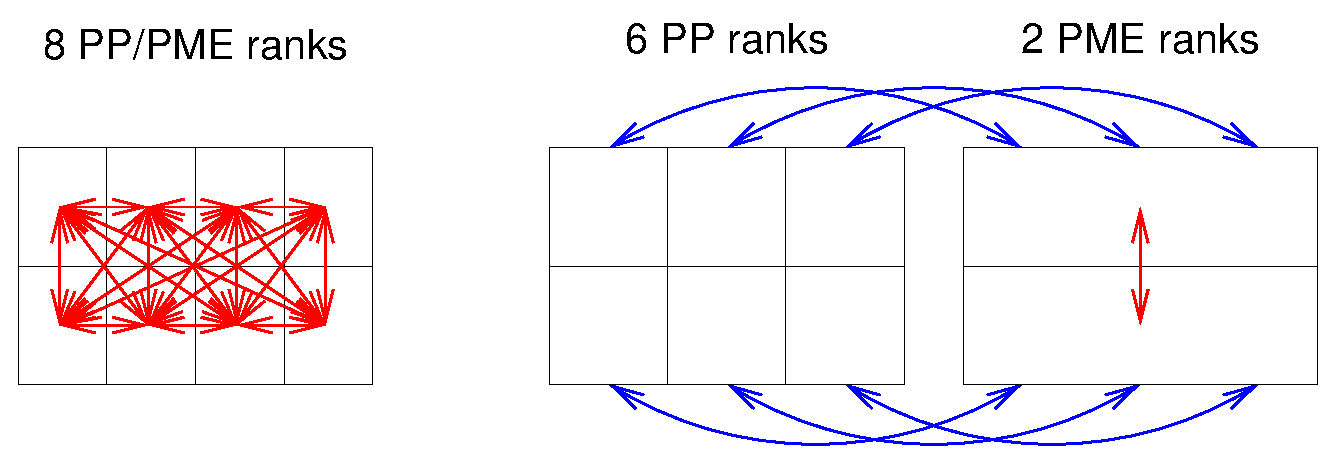
\includegraphics[width=12cm]{plots/mpmd-pme}}
\caption{
Example of 8 ranks without (left) and with (right) MPMD.
The PME communication (red arrows) is much higher on the left
than on the right. For MPMD additional PP - PME coordinate
and force communication (blue arrows) is required,
but the total communication complexity is lower.
\label{fig:mpmd_pme}
}
\end{figure}

{\tt mdrun} will by default interleave the PP and PME ranks.
If the ranks are not number consecutively inside the machines,
one might want to use {\tt mdrun -ddorder pp_pme}.
For machines with a real 3-D torus and proper communication software
that assigns the ranks accordingly one should use
{\tt mdrun -ddorder cartesian}.

To optimize the performance one should usually set up the cut-offs
and the PME grid such that the PME load is 25 to 33\% of the total
calculation load. {\tt grompp} will print an estimate for this load
at the end and also {\tt mdrun} calculates the same estimate
to determine the optimal number of PME ranks to use.
For high parallelization it might be worthwhile to optimize
the PME load with the {\tt mdp} settings and/or the number
of PME ranks with the {\tt -npme} option of {\tt mdrun}.
For changing the electrostatics settings it is useful to know
the accuracy of the electrostatics remains nearly constant
when the Coulomb cut-off and the PME grid spacing are scaled
by the same factor.
{\bf Note} that it is usually better to overestimate than to underestimate
the number of PME ranks, since the number of PME ranks is smaller
than the number of PP ranks, which leads to less total waiting time.

The PME domain decomposition can be 1-D or 2-D along the $x$ and/or
$y$ axis. 2-D decomposition is also known as \normindex{pencil decomposition} because of
the shape of the domains at high parallelization.
1-D decomposition along the $y$ axis can only be used when
the PP decomposition has only 1 domain along $x$. 2-D PME decomposition
has to have the number of domains along $x$ equal to the number of
the PP decomposition. {\tt mdrun} automatically chooses 1-D or 2-D
PME decomposition (when possible with the total given number of ranks),
based on the minimum amount of communication for the coordinate redistribution
in PME plus the communication for the grid overlap and transposes.
To avoid superfluous communication of coordinates and forces
between the PP and PME ranks, the number of DD cells in the $x$
direction should ideally be the same or a multiple of the number
of PME ranks. By default, {\tt mdrun} takes care of this issue.

\subsection{Domain decomposition flow chart}
In \figref{dd_flow} a flow chart is shown for domain decomposition
with all possible communication for different algorithms.
For simpler simulations, the same flow chart applies,
without the algorithms and communication for
the algorithms that are not used.

\begin{figure}
\centerline{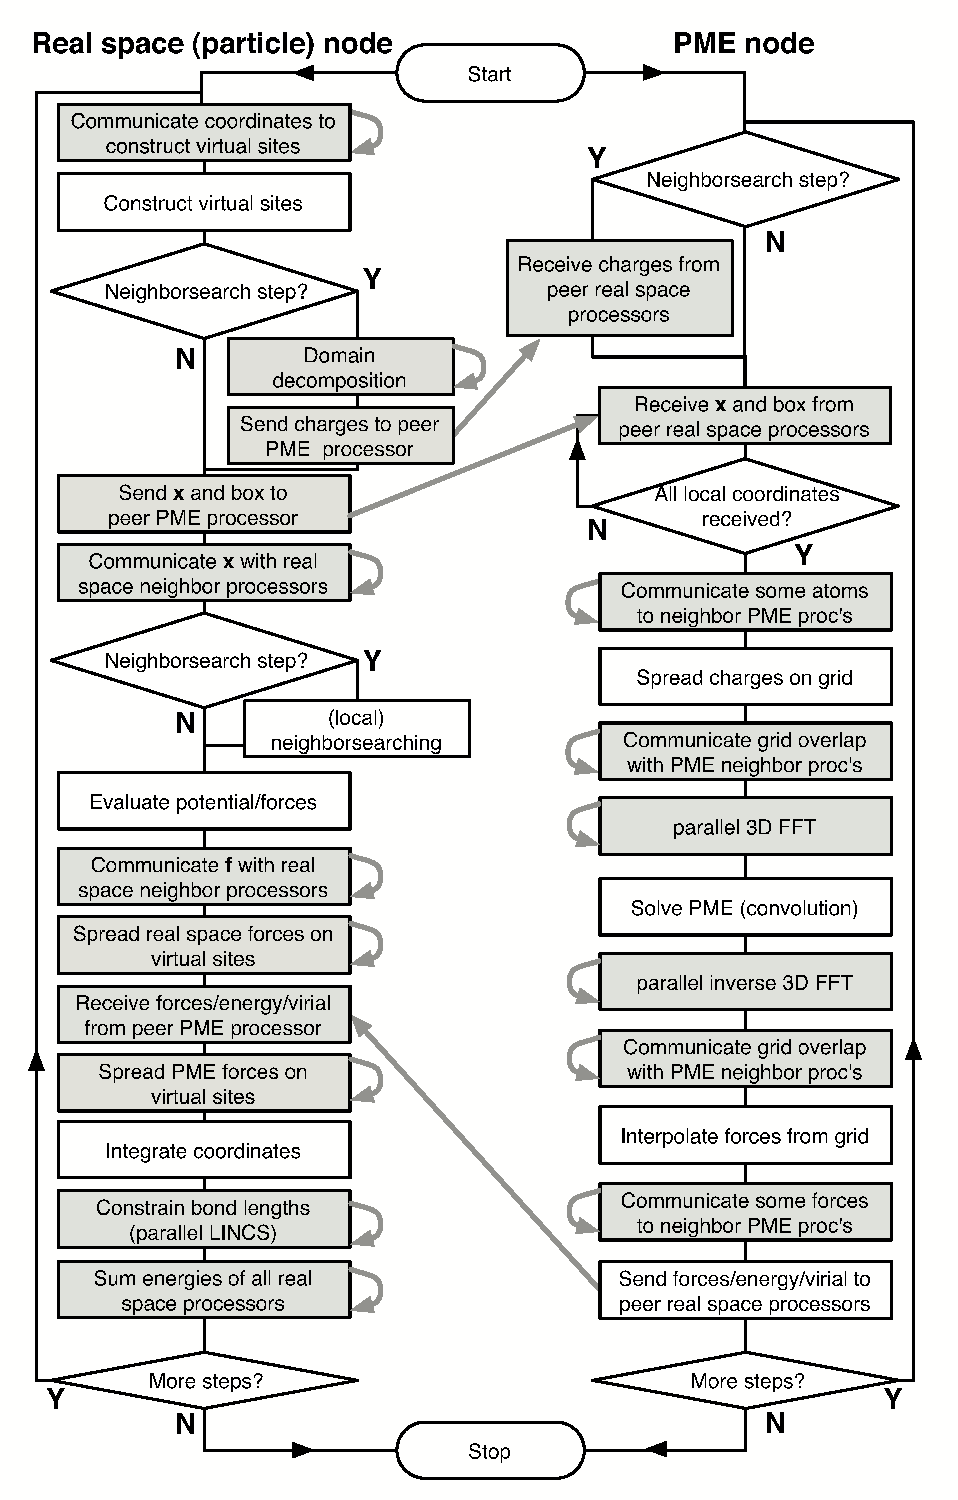
\includegraphics[width=12cm]{plots/flowchart}}
\caption{
Flow chart showing the algorithms and communication (arrows)
for a standard MD simulation with virtual sites, constraints
and separate PME-mesh ranks.
\label{fig:dd_flow}
}
\end{figure}


\section{Implicit solvation\index{implicit solvation}\index{Generalized Born methods}}
\label{sec:gbsa}
Implicit solvent models provide an efficient way of representing 
the electrostatic effects of solvent molecules, while saving a 
large piece of the computations involved in an accurate, aqueous 
description of the surrounding water in molecular dynamics simulations. 
Implicit solvation models offer several advantages compared with 
explicit solvation, including eliminating the need for the equilibration of water 
around the solute, and the absence of viscosity, which allows the protein 
to more quickly explore conformational space.

Implicit solvent calculations in {\gromacs} can be done using the 
generalized Born-formalism, and the Still~\cite{Still97}, HCT~\cite{Truhlar96}, 
and OBC~\cite{Case04} models are available for calculating the Born radii.

Here, the free energy $G_{\mathrm{solv}}$ of solvation is the sum of three terms,
a solvent-solvent cavity term ($G_{\mathrm{cav}}$), a solute-solvent van der
Waals term ($G_{\mathrm{vdw}}$), and finally a solvent-solute electrostatics
polarization term ($G_{\mathrm{pol}}$).

The sum of $G_{\mathrm{cav}}$ and $G_{\mathrm{vdw}}$ corresponds to the (non-polar)
free energy of solvation for a molecule from which all charges
have been removed, and is commonly called $G_{\mathrm{np}}$,
calculated from the total solvent accessible surface area 
multiplied with a surface tension. 
The total expression for the solvation free energy then becomes:

\beq
G_{\mathrm{solv}} = G_{\mathrm{np}}  + G_{\mathrm{pol}}
\label{eqn:gb_solv}
\eeq

Under the generalized Born model, $G_{\mathrm{pol}}$ is calculated from the generalized Born equation~\cite{Still97}:

\beq
G_{\mathrm{pol}} = \left(1-\frac{1}{\epsilon}\right) \sum_{i=1}^n \sum_{j>i}^n \frac {q_i q_j}{\sqrt{r^2_{ij} + b_i b_j \exp\left(\frac{-r^2_{ij}}{4 b_i b_j}\right)}}
\label{eqn:gb_still}
\eeq

In {\gromacs}, we have introduced the substitution~\cite{Larsson10}:

\beq
c_i=\frac{1}{\sqrt{b_i}}
\label{eqn:gb_subst}
\eeq

which makes it possible to introduce a cheap transformation to a new 
variable $x$ when evaluating each interaction, such that:

\beq
x=\frac{r_{ij}}{\sqrt{b_i b_j }} = r_{ij} c_i c_j
\label{eqn:gb_subst2}
\eeq

In the end, the full re-formulation of~\ref{eqn:gb_still} becomes:
 
\beq
G_{\mathrm{pol}} = \left(1-\frac{1}{\epsilon}\right) \sum_{i=1}^n \sum_{j>i}^n \frac{q_i q_j}{\sqrt{b_i  b_j}} ~\xi (x) = \left(1-\frac{1}{\epsilon}\right) \sum_{i=1}^n q_i c_i \sum_{j>i}^n q_j c_j~\xi (x)
\label{eqn:gb_final}
\eeq 

The non-polar part ($G_{\mathrm{np}}$) of Equation~\ref{eqn:gb_solv} is calculated 
directly from the Born radius of each atom using a simple ACE type 
approximation by Schaefer {\em et al.}~\cite{Karplus98}, including a 
simple loop over all atoms. 
This requires only one extra solvation parameter, independent of atom type, 
but differing slightly between the three Born radii models.

% LocalWords:  GROningen MAchine BIOSON Groningen GROMACS Berendsen der Spoel
% LocalWords:  Drunen Comp Phys Comm ROck NS FFT pbc EM ifthenelse gmxlite ff
% LocalWords:  octahedra triclinic Ewald PME PPPM trjconv xy solvated
% LocalWords:  boxtypes boxshapes editconf Lennard COM XTC TNG kT defunits
% LocalWords:  Boltzmann's Mueller nb int mdrun chargegroup simplerc prefactor
% LocalWords:  pme waterloops CH NH CO df com virial integrator Verlet vverlet
% LocalWords:  integrators ref timepoint timestep timesteps mdp md vv avek NVE
% LocalWords:  NVT off's leapfrogv lll LR rmfast SPC fs Nos physicality ps GMX
% LocalWords:  Tcoupling nonergodic thermostatting NOSEHOOVER algorithmes ij yx
% LocalWords:  Parrinello Rahman rescales atm anisotropically ccc xz zx yy yz
% LocalWords:  zy zz se barostat compressibilities MTTK NPT Martyna al isobaric
% LocalWords:  Tuckerman vir PV fkT iLt iL Liouville NHC Eq baro mu trj mol bc
% LocalWords:  freezegroup Shannon's polarizability Overhauser barostats iLn KE
% LocalWords:  negligibly thermostatted Tobias  rhombic maxwell et xtc tng TC rlist
% LocalWords:  waals LINCS holonomic plincs lincs unc ang SA Langevin SD amu BD
% LocalWords:  bfgs Broyden Goldfarb Shanno mkT kJ DFLEXIBLE Nocedal diag nmeig
% LocalWords:  diagonalization anaeig nmens covanal ddg feia BT dp dq pV dV dA
% LocalWords:  NpT eq stepsize REMD constrainted website Okabe MPI covar edi dd
% LocalWords:  progman NMR ddcells innerloops ddtric tric dds rdd conf rcon est
% LocalWords:  mb PP MPMD ddorder pp cartesian grompp npme parallelizable edr
% LocalWords:  macromolecule nstlist vacuo parallelization dof indices MBAR AVX
% LocalWords:  TOL numerics parallelized eigenvectors dG parallelepipeds VdW np
% LocalWords:  Coul multi solvation HCT OBC solv cav vdw Schaefer symplectic dt
% LocalWords:  pymbar multinode subensemble Monte solute subst groupconcept GPU
% LocalWords:  dodecahedron octahedron dodecahedra equilibration usinggroups nm
% LocalWords:  topologies rlistlong CUDA GPUs rcoulomb SIMD BlueGene FPUs erfc
% LocalWords:  cutoffschemesupport unbuffered bondeds OpenMP ewald rtol
% LocalWords:  verletdrift peptide RMS rescaling ergodicity ergodic discretized
% LocalWords:  isothermal compressibility isotropically anisotropic iteratively
% LocalWords:  incompressible integrations translational biomolecules NMA PCA
% LocalWords:  Bennett's equilibrated Hamiltonians covariance equilibrate
% LocalWords:  inhomogeneous conformational online other's th

%
% This file is part of the GROMACS molecular simulation package.
%
% Copyright (c) 2013,2014,2015,2016, by the GROMACS development team, led by
% Mark Abraham, David van der Spoel, Berk Hess, and Erik Lindahl,
% and including many others, as listed in the AUTHORS file in the
% top-level source directory and at http://www.gromacs.org.
%
% GROMACS is free software; you can redistribute it and/or
% modify it under the terms of the GNU Lesser General Public License
% as published by the Free Software Foundation; either version 2.1
% of the License, or (at your option) any later version.
%
% GROMACS is distributed in the hope that it will be useful,
% but WITHOUT ANY WARRANTY; without even the implied warranty of
% MERCHANTABILITY or FITNESS FOR A PARTICULAR PURPOSE.  See the GNU
% Lesser General Public License for more details.
%
% You should have received a copy of the GNU Lesser General Public
% License along with GROMACS; if not, see
% http://www.gnu.org/licenses, or write to the Free Software Foundation,
% Inc., 51 Franklin Street, Fifth Floor, Boston, MA  02110-1301  USA.
%
% If you want to redistribute modifications to GROMACS, please
% consider that scientific software is very special. Version
% control is crucial - bugs must be traceable. We will be happy to
% consider code for inclusion in the official distribution, but
% derived work must not be called official GROMACS. Details are found
% in the README & COPYING files - if they are missing, get the
% official version at http://www.gromacs.org.
%
% To help us fund GROMACS development, we humbly ask that you cite
% the research papers on the package. Check out http://www.gromacs.org.

\chapter{Interaction function and force fields\index{force field}}
\label{ch:ff}
To accommodate the potential functions used
in some popular force fields (see \ref{sec:ff}), {\gromacs} offers a choice of functions,
both for non-bonded interaction and for dihedral interactions. They
are described in the appropriate subsections.

The potential functions can be subdivided into three parts
\begin{enumerate}
\item   {\em Non-bonded}: Lennard-Jones or Buckingham, and Coulomb or
modified Coulomb. The non-bonded interactions are computed on the
basis of a neighbor list (a list of non-bonded atoms within a certain
radius), in which exclusions are already removed.
\item   {\em Bonded}: covalent bond-stretching, angle-bending,
improper dihedrals, and proper dihedrals. These are computed on the
basis of fixed lists. 
\item   {\em Restraints}: position restraints, angle restraints,
distance restraints, orientation restraints and dihedral restraints, all
based on fixed lists. 
\end{enumerate}

\section{Non-bonded interactions}
Non-bonded interactions in {\gromacs} are pair-additive and centro-symmetric:
\beq
V(\ve{r}_1,\ldots \ve{r}_N) = \sum_{i<j}V_{ij}(\rvij);
\eeq
\beq
\ve{F}_i = -\sum_j \frac{dV_{ij}(r_{ij})}{dr_{ij}} \frac{\rvij}{r_{ij}} = -\ve{F}_j
\eeq
The non-bonded interactions contain a \normindex{repulsion} term, 
a \normindex{dispersion}
term, and a Coulomb term. The repulsion and dispersion term are
combined in either the Lennard-Jones (or 6-12 interaction), or the
Buckingham (or exp-6 potential). In addition, (partially) charged atoms
act through the Coulomb term. 

\subsection{The Lennard-Jones interaction}
\label{sec:lj}
The \normindex{Lennard-Jones} potential $V_{LJ}$ between two atoms equals:
\beq
V_{LJ}(\rij) =  \frac{C_{ij}^{(12)}}{\rij^{12}} -
                        \frac{C_{ij}^{(6)}}{\rij^6}     
\eeq
See also \figref{lj}
The parameters $C^{(12)}_{ij}$ and $C^{(6)}_{ij}$  depend on pairs of
{\em atom types}; consequently they are taken from a matrix of
LJ-parameters. In the Verlet cut-off scheme, the potential is shifted
by a constant such that it is zero at the cut-off distance.

\begin{figure}
\centerline{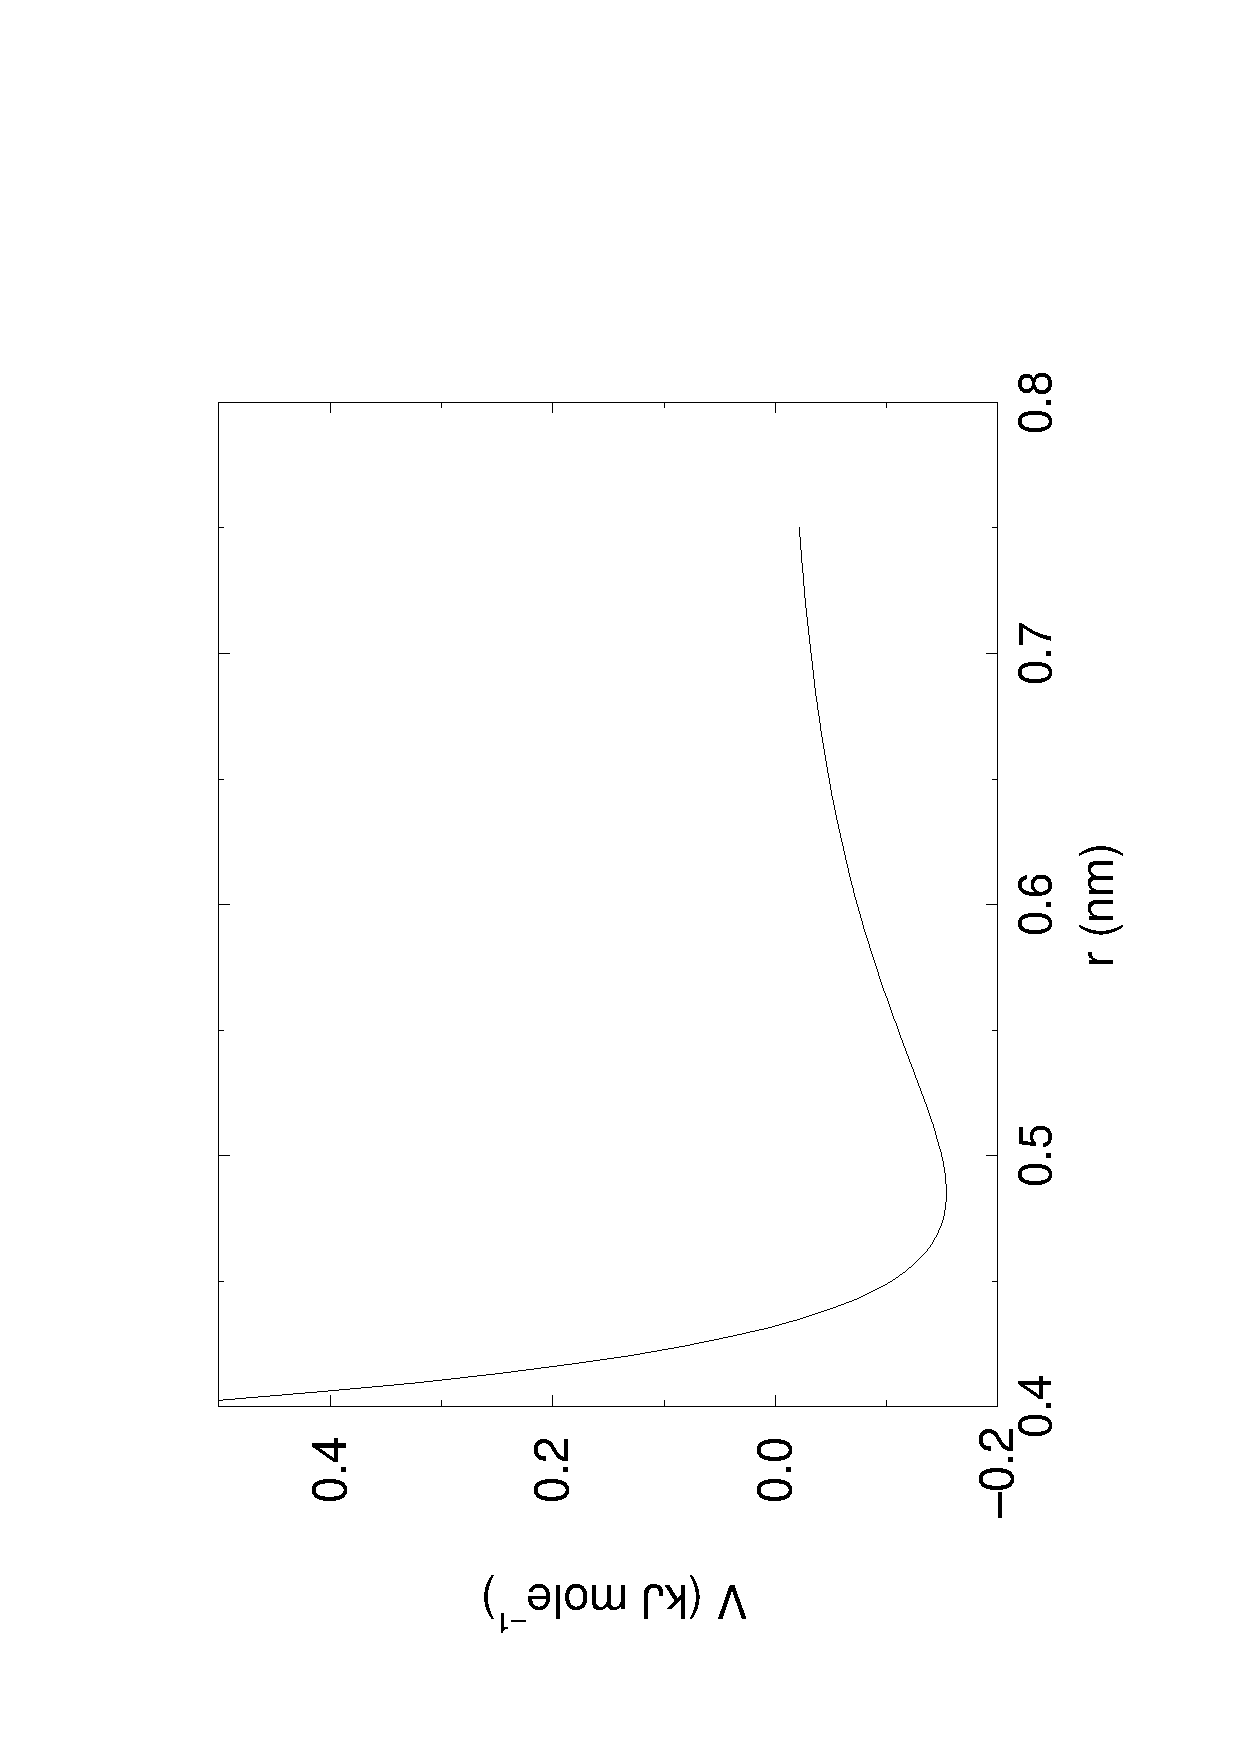
\includegraphics[width=8cm]{plots/f-lj}}
\caption {The Lennard-Jones interaction.}
\label{fig:lj}
\end{figure}
 
The force derived from this potential is:
\beq
\ve{F}_i(\rvij) = \left( 12~\frac{C_{ij}^{(12)}}{\rij^{13}} -
                                 6~\frac{C_{ij}^{(6)}}{\rij^7} \right) \rnorm 
\eeq

The LJ potential may also be written in the following form:
\beq
V_{LJ}(\rvij) = 4\epsilon_{ij}\left(\left(\frac{\sigma_{ij}} {\rij}\right)^{12}
                - \left(\frac{\sigma_{ij}}{\rij}\right)^{6} \right)
\label{eqn:sigeps}      
\eeq

In constructing the parameter matrix for the non-bonded LJ-parameters,
two types of \normindex{combination rule}s can be used within {\gromacs},
only geometric averages (type 1 in the input section of the force-field file):
\beq
\begin{array}{rcl}
C_{ij}^{(6)}    &=& \left({C_{ii}^{(6)} \, C_{jj}^{(6)}}\right)^{1/2}    \\
C_{ij}^{(12)}   &=& \left({C_{ii}^{(12)} \, C_{jj}^{(12)}}\right)^{1/2}
\label{eqn:comb}
\end{array}
\eeq
or, alternatively the Lorentz-Berthelot rules can be used. An arithmetic average is used to calculate $\sigma_{ij}$, while a geometric average is used to calculate $\epsilon_{ij}$ (type 2):
\beq
\begin{array}{rcl}
 \sigma_{ij}   &=& \frac{1}{ 2}(\sigma_{ii} + \sigma_{jj})        \\
 \epsilon_{ij} &=& \left({\epsilon_{ii} \, \epsilon_{jj}}\right)^{1/2}
 \label{eqn:lorentzberthelot}
\end{array}
\eeq
finally an geometric average for both parameters can be used (type 3):
\beq
\begin{array}{rcl}
 \sigma_{ij}   &=& \left({\sigma_{ii} \, \sigma_{jj}}\right)^{1/2}        \\
 \epsilon_{ij} &=& \left({\epsilon_{ii} \, \epsilon_{jj}}\right)^{1/2}
\end{array}
\eeq
This last rule is used by the OPLS force field.


%\ifthenelse{\equal{\gmxlite}{1}}{}{
\subsection{\normindex{Buckingham potential}}
The Buckingham
potential has a more flexible and realistic repulsion term
than the Lennard-Jones interaction, but is also more expensive to
compute. The potential form is:
\beq
V_{bh}(\rij) = A_{ij} \exp(-B_{ij} \rij) -
                        \frac{C_{ij}}{\rij^6}
\eeq
\begin{figure}
\centerline{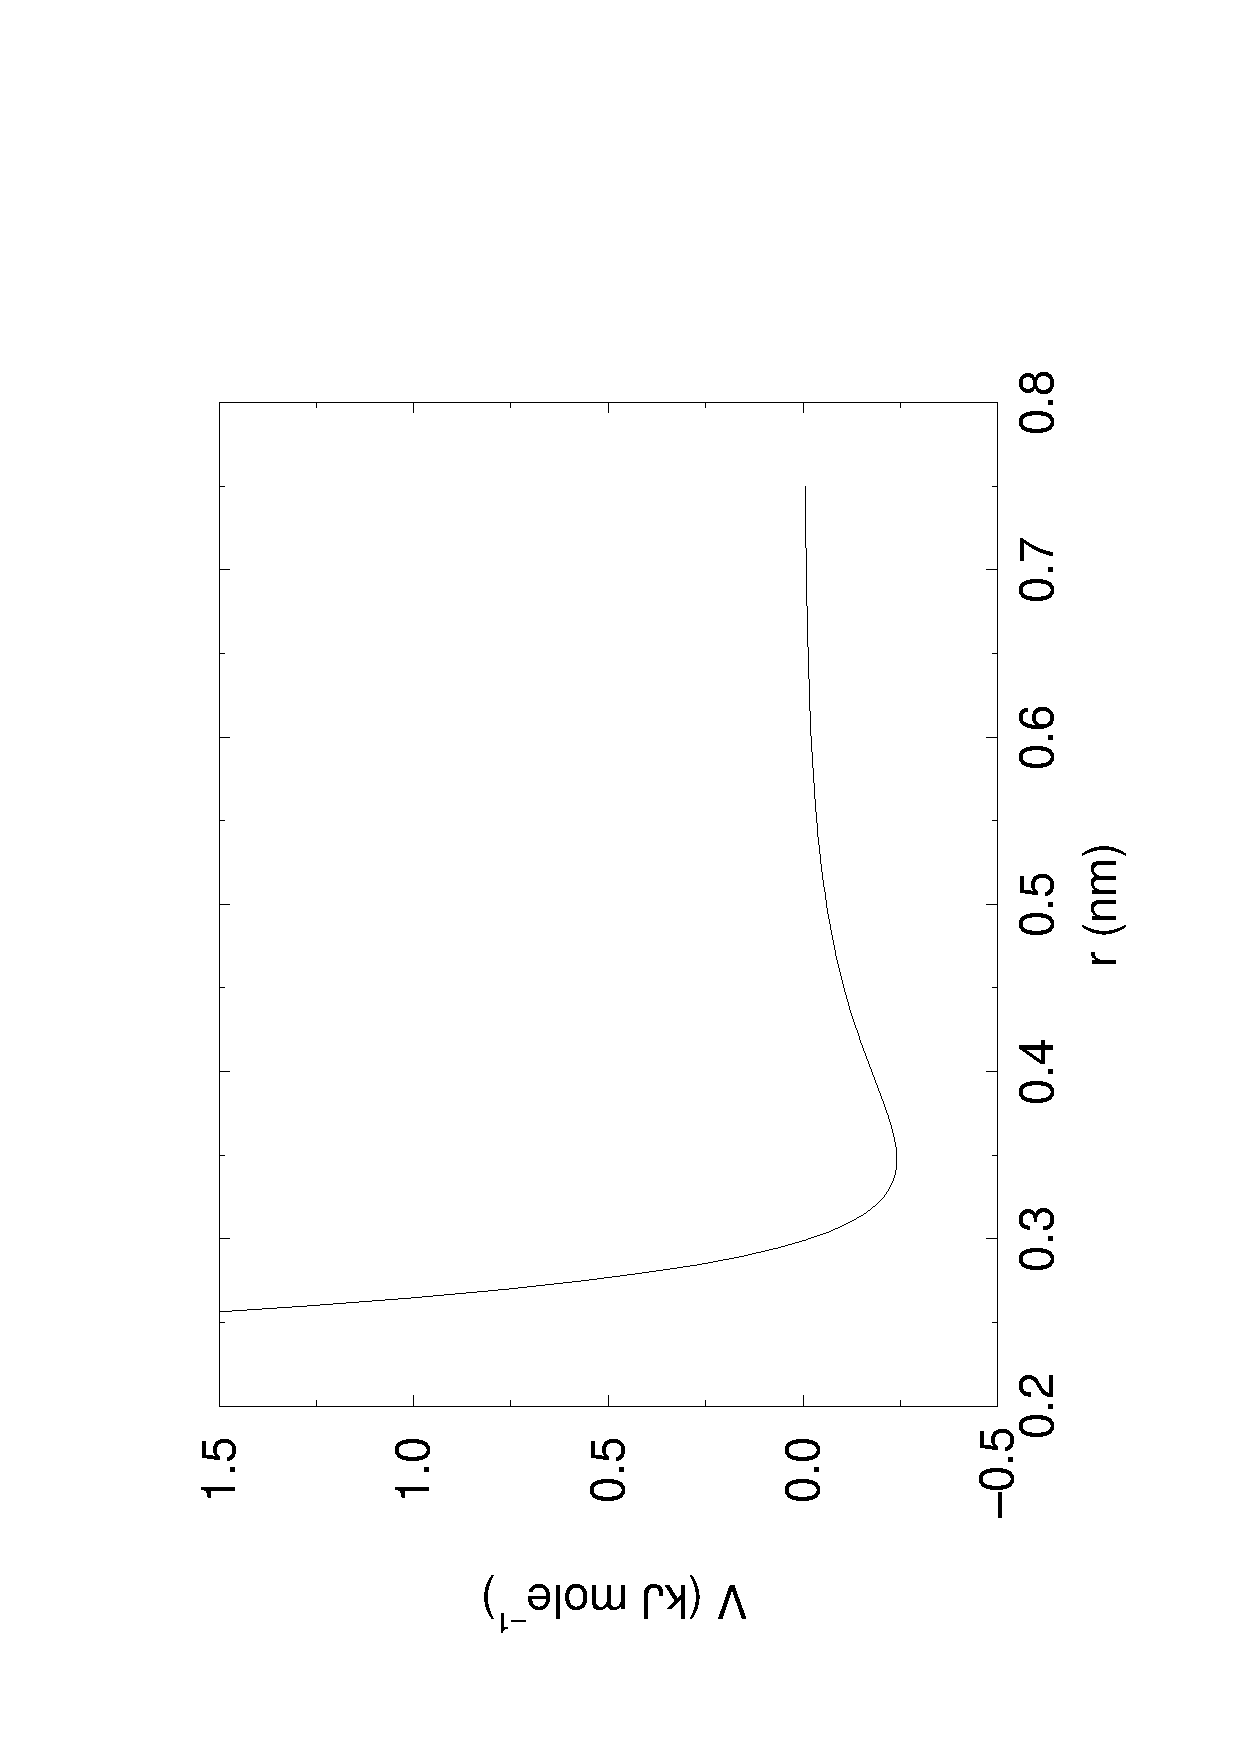
\includegraphics[width=8cm]{plots/f-bham}}
\caption {The Buckingham interaction.}
\label{fig:bham}
\end{figure}

See also \figref{bham}.  The force derived from this is:
\beq
 \ve{F}_i(\rij) = \left[ A_{ij}B_{ij}\exp(-B_{ij} \rij) -
                                 6\frac{C_{ij}}{\rij^7} \right] \rnorm
\eeq

%} % Brace matches ifthenelse test for gmxlite

\subsection{Coulomb interaction}
\label{sec:coul}
\newcommand{\epsr}{\varepsilon_r}
\newcommand{\epsrf}{\varepsilon_{rf}}
The \normindex{Coulomb} interaction between two charge particles is given by:
\beq
V_c(\rij) = f \frac{q_i q_j}{\epsr \rij}
\label{eqn:vcoul}
\eeq
See also \figref{coul}, where $f = \frac{1}{4\pi \varepsilon_0} =
\electricConvFactorValue$ (see \chref{defunits})

\begin{figure}
\centerline{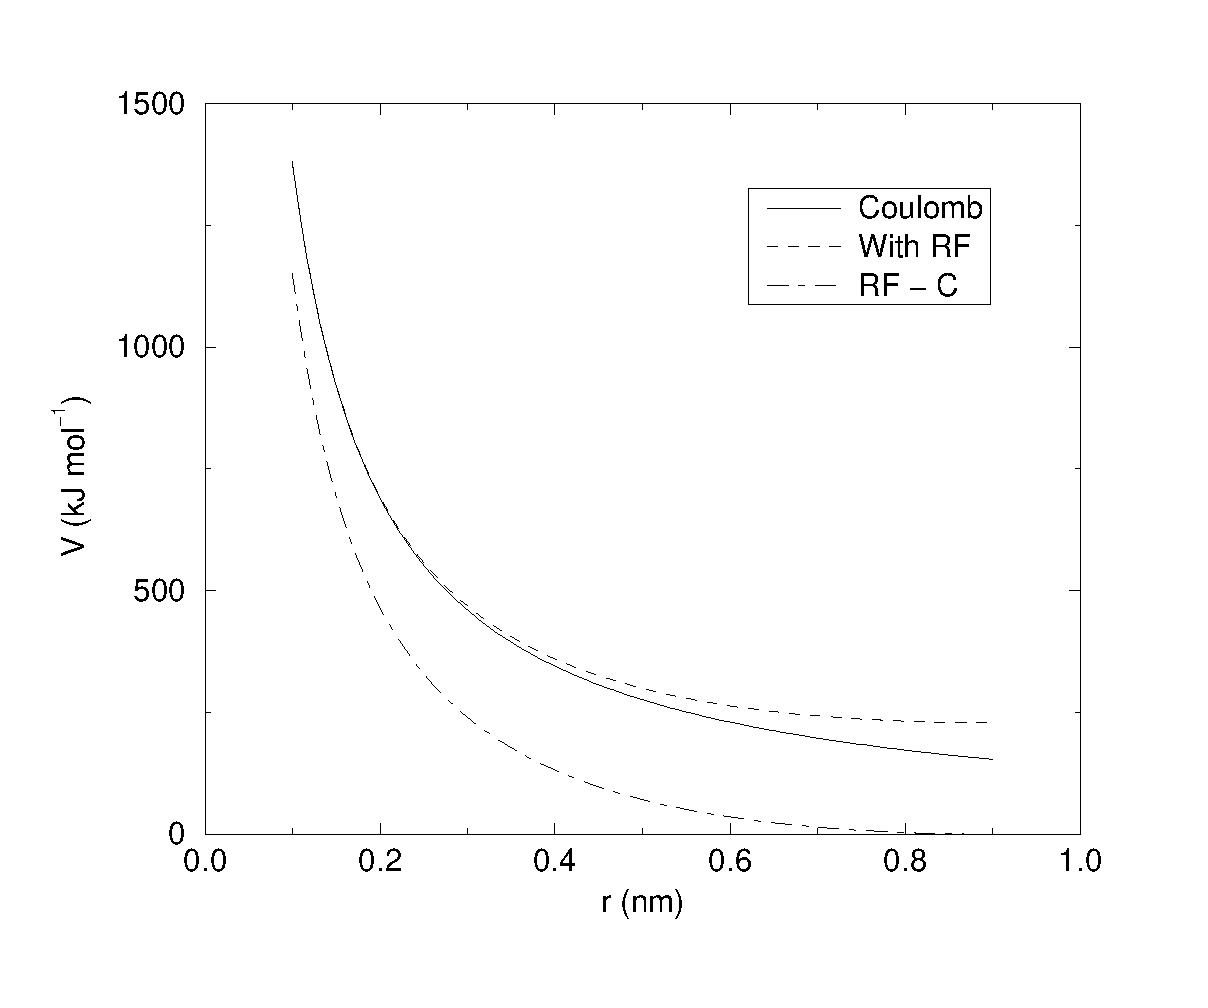
\includegraphics[width=8cm]{plots/vcrf}}
\caption[The Coulomb interaction with and without reaction field.]{The
Coulomb interaction (for particles with equal signed charge) with and
without reaction field. In the latter case $\epsr$ was 1, $\epsrf$ was 78,
and $r_c$ was 0.9 nm.
The dot-dashed line is the same as the dashed line, except for a constant.}
\label{fig:coul}
\end{figure}

The force derived from this potential is:
\beq
\ve{F}_i(\rvij) = f \frac{q_i q_j}{\epsr\rij^2}\rnorm
\eeq

A plain Coulomb interaction should only be used without cut-off or when all pairs fall within the cut-off, since there is an abrupt, large change in the force at the cut-off. In case you do want to use a cut-off, the potential can be shifted by a constant to make the potential the integral of the force. With the group cut-off scheme, this shift is only applied to non-excluded pairs. With the Verlet cut-off scheme, the shift is also applied to excluded pairs and self interactions, which makes the potential equivalent to a reaction field with $\epsrf=1$ (see below).

In {\gromacs} the  relative \swapindex{dielectric}{constant} 
\normindex{$\epsr$}
may be set in the in the input for {\tt grompp}. 

%\ifthenelse{\equal{\gmxlite}{1}}{}{
\subsection{Coulomb interaction with \normindex{reaction field}}
\label{sec:coulrf}
The Coulomb interaction can be modified for homogeneous systems by
assuming a constant dielectric environment beyond the cut-off $r_c$
with a dielectric constant of {$\epsrf$}. The interaction then reads:
\beq
V_{crf} ~=~
  f \frac{q_i q_j}{\epsr\rij}\left[1+\frac{\epsrf-\epsr}{2\epsrf+\epsr}
  \,\frac{\rij^3}{r_c^3}\right]
  - f\frac{q_i q_j}{\epsr r_c}\,\frac{3\epsrf}{2\epsrf+\epsr}
\label{eqn:vcrf}
\eeq
in which the constant expression on the right makes the potential
zero at the cut-off $r_c$. For charged cut-off spheres this corresponds
to neutralization with a homogeneous background charge.
We can rewrite \eqnref{vcrf} for simplicity as
\beq
V_{crf} ~=~     f \frac{q_i q_j}{\epsr}\left[\frac{1}{\rij} + k_{rf}~ \rij^2 -c_{rf}\right]
\eeq
with
\bea
k_{rf}  &=&     \frac{1}{r_c^3}\,\frac{\epsrf-\epsr}{(2\epsrf+\epsr)}   \label{eqn:krf}\\
c_{rf}  &=&     \frac{1}{r_c}+k_{rf}\,r_c^2 ~=~ \frac{1}{r_c}\,\frac{3\epsrf}{(2\epsrf+\epsr)}
\label{eqn:crf}
\eea
For large $\epsrf$ the $k_{rf}$ goes to $r_c^{-3}/2$,
while for $\epsrf$ = $\epsr$ the correction vanishes.
In \figref{coul}
the modified interaction is plotted, and it is clear that the derivative 
with respect to $\rij$ (= -force) goes to zero at the cut-off distance.
The force derived from this potential reads:
\beq
\ve{F}_i(\rvij) = f \frac{q_i q_j}{\epsr}\left[\frac{1}{\rij^2} - 2 k_{rf}\rij\right]\rnorm
\label{eqn:fcrf}
\eeq
The reaction-field correction should also be applied to all excluded
atoms pairs, including self pairs, in which case the normal Coulomb
term in \eqnsref{vcrf}{fcrf} is absent.

Tironi {\etal} have introduced a generalized reaction field in which
the dielectric continuum beyond the cut-off $r_c$ also has an ionic strength
$I$~\cite{Tironi95}. In this case we can rewrite the constants $k_{rf}$ and 
$c_{rf}$ using the inverse Debye screening length $\kappa$:
\bea
\kappa^2  &=&     
   \frac{2 I \,F^2}{\varepsilon_0 \epsrf RT}
   = \frac{F^2}{\varepsilon_0 \epsrf RT}\sum_{i=1}^{K} c_i z_i^2     \\
k_{rf}  &=&     \frac{1}{r_c^3}\,
    \frac{(\epsrf-\epsr)(1 + \kappa r_c) + \half\epsrf(\kappa r_c)^2}
         {(2\epsrf + \epsr)(1 + \kappa r_c) + \epsrf(\kappa r_c)^2}
    \label{eqn:kgrf}\\
c_{rf}  &=&     \frac{1}{r_c}\,
    \frac{3\epsrf(1 + \kappa r_c + \half(\kappa r_c)^2)}
         {(2\epsrf+\epsr)(1 + \kappa r_c) + \epsrf(\kappa r_c)^2}
    \label{eqn:cgrf}
\eea
where $F$ is Faraday's constant, $R$ is the ideal gas constant, $T$
the absolute temperature, $c_i$ the molar concentration for species
$i$ and $z_i$ the charge number of species $i$ where we have $K$
different species. In the limit of zero ionic strength ($\kappa=0$)
\eqnsref{kgrf}{cgrf} reduce to the simple forms of \eqnsref{krf}{crf}
respectively.

\subsection{Modified non-bonded interactions}
\label{sec:mod_nb_int}
In {\gromacs}, the non-bonded potentials can be
modified by a shift function, also called a force-switch function,
since it switches the force to zero at the cut-off.
The purpose of this is to replace the
truncated forces by forces that are continuous and have continuous
derivatives at the \normindex{cut-off} radius. With such forces the
time integration produces smaller errors. But note that for
Lennard-Jones interactions these errors are usually smaller than other errors,
such as integration errors at the repulsive part of the potential.
For Coulomb interactions we advise against using a shifted potential
and for use of a reaction field or a proper long-range method such as PME.
 
There is {\em no} fundamental difference between a switch function
(which multiplies the potential with a function) and a shift function
(which adds a function to the force or potential)~\cite{Spoel2006a}. The switch
function is a special case of the shift function, which we apply to
the {\em force function} $F(r)$, related to the electrostatic or
van der Waals force acting on particle $i$ by particle $j$ as:
\beq
\ve{F}_i = c \, F(r_{ij}) \frac{\rvij}{r_{ij}}
\eeq
For pure Coulomb or Lennard-Jones interactions
$F(r) = F_\alpha(r) = \alpha \, r^{-(\alpha+1)}$.
The switched force $F_s(r)$ can generally be written as:
\beq
\begin{array}{rcl}
\vspace{2mm}
F_s(r)~=&~F_\alpha(r)   & r < r_1               \\
\vspace{2mm}
F_s(r)~=&~F_\alpha(r)+S(r)      & r_1 \le r < r_c       \\
F_s(r)~=&~0             & r_c \le r     
\end{array}
\eeq
When $r_1=0$ this is a traditional shift function, otherwise it acts as a 
switch function. The corresponding shifted potential function then reads:
\beq
V_s(r) =  \int^{\infty}_r~F_s(x)\, dx
\eeq

The {\gromacs} {\bf force switch} function $S_F(r)$ should be smooth at the boundaries, therefore
the following boundary conditions are imposed on the switch function:
\beq
\begin{array}{rcl}
S_F(r_1)          &=&0            \\
S_F'(r_1)         &=&0            \\
S_F(r_c)          &=&-F_\alpha(r_c)       \\
S_F'(r_c)         &=&-F_\alpha'(r_c)
\end{array}
\eeq
A 3$^{rd}$ degree polynomial of the form
\beq
S_F(r) = A(r-r_1)^2 + B(r-r_1)^3
\eeq
fulfills these requirements. The constants A and B are given by the
boundary condition at $r_c$: 
\beq
\begin{array}{rcl}
\vspace{2mm}
A &~=~& -\alpha \, \displaystyle
        \frac{(\alpha+4)r_c~-~(\alpha+1)r_1} {r_c^{\alpha+2}~(r_c-r_1)^2} \\
B &~=~& \alpha \, \displaystyle
        \frac{(\alpha+3)r_c~-~(\alpha+1)r_1}{r_c^{\alpha+2}~(r_c-r_1)^3}
\end{array}
\eeq
Thus the total force function is:
\beq
F_s(r) = \frac{\alpha}{r^{\alpha+1}} + A(r-r_1)^2 + B(r-r_1)^3
\eeq
and the potential function reads:
\beq
V_s(r) = \frac{1}{r^\alpha} - \frac{A}{3} (r-r_1)^3 - \frac{B}{4} (r-r_1)^4 - C
\eeq
where 
\beq
C =  \frac{1}{r_c^\alpha} - \frac{A}{3} (r_c-r_1)^3 - \frac{B}{4} (r_c-r_1)^4
\eeq

The {\gromacs} {\bf potential-switch} function $S_V(r)$ scales the potential between
$r_1$ and $r_c$, and has similar boundary conditions, intended to produce
smoothly-varying potential and forces:
\beq
\begin{array}{rcl}
S_V(r_1)          &=&1 \\
S_V'(r_1)         &=&0 \\
S_V''(r_1)        &=&0 \\
S_V(r_c)          &=&0 \\
S_V'(r_c)         &=&0 \\
S_V''(r_c)        &=&0
\end{array}
\eeq

The fifth-degree polynomial that has these properties is
\beq
S_V(r; r_1, r_c) = \frac{1 - 10(r-r_1)^3(r_c-r_1)^2 + 15(r-r_1)^4(r_c-r_1) - 6(r-r_1)}{(r_c-r_1)^5}
\eeq

This implementation is found in several other simulation
packages,\cite{Ohmine1988,Kitchen1990,Guenot1993} but differs from
that in CHARMM.\cite{Steinbach1994} Switching the potential leads to
artificially large forces in the switching region, therefore it is not
recommended to switch Coulomb interactions using this
function,\cite{Spoel2006a} but switching Lennard-Jones interactions
using this function produces acceptable results.

\subsection{Modified short-range interactions with Ewald summation}
When Ewald summation\index{Ewald sum} or \seeindex{particle-mesh
Ewald}{PME}\index{Ewald, particle-mesh} is used to calculate the
long-range interactions, the 
short-range Coulomb potential must also be modified. Here the potential
is switched to (nearly) zero at the cut-off, instead of the force.
In this case the short range potential is given by:
\beq
V(r) = f \frac{\mbox{erfc}(\beta r_{ij})}{r_{ij}} q_i q_j,
\eeq
where $\beta$ is a parameter that determines the relative weight 
between the direct space sum and the reciprocal space sum and erfc$(x)$ is
the complementary error function. For further 
details on long-range electrostatics, see \secref{lr_elstat}.
%} % Brace matches ifthenelse test for gmxlite


\section{Bonded interactions}
Bonded interactions are based on a fixed list of atoms. They are not
exclusively pair interactions, but include 3- and 4-body interactions
as well. There are {\em bond stretching} (2-body), {\em bond angle}
(3-body), and {\em dihedral angle} (4-body) interactions. A special
type of dihedral interaction (called {\em improper dihedral}) is used
to force atoms to remain in a plane or to prevent transition to a
configuration of opposite chirality (a mirror image).

\subsection{Bond stretching}
\label{sec:bondpot}
\subsubsection{Harmonic potential}
\label{subsec:harmonicbond}
The \swapindex{bond}{stretching} between two covalently bonded atoms
$i$ and $j$ is represented by a harmonic potential:

\begin{figure}
\centerline{\raisebox{2cm}{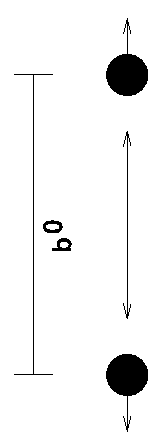
\includegraphics[width=5cm]{plots/bstretch}}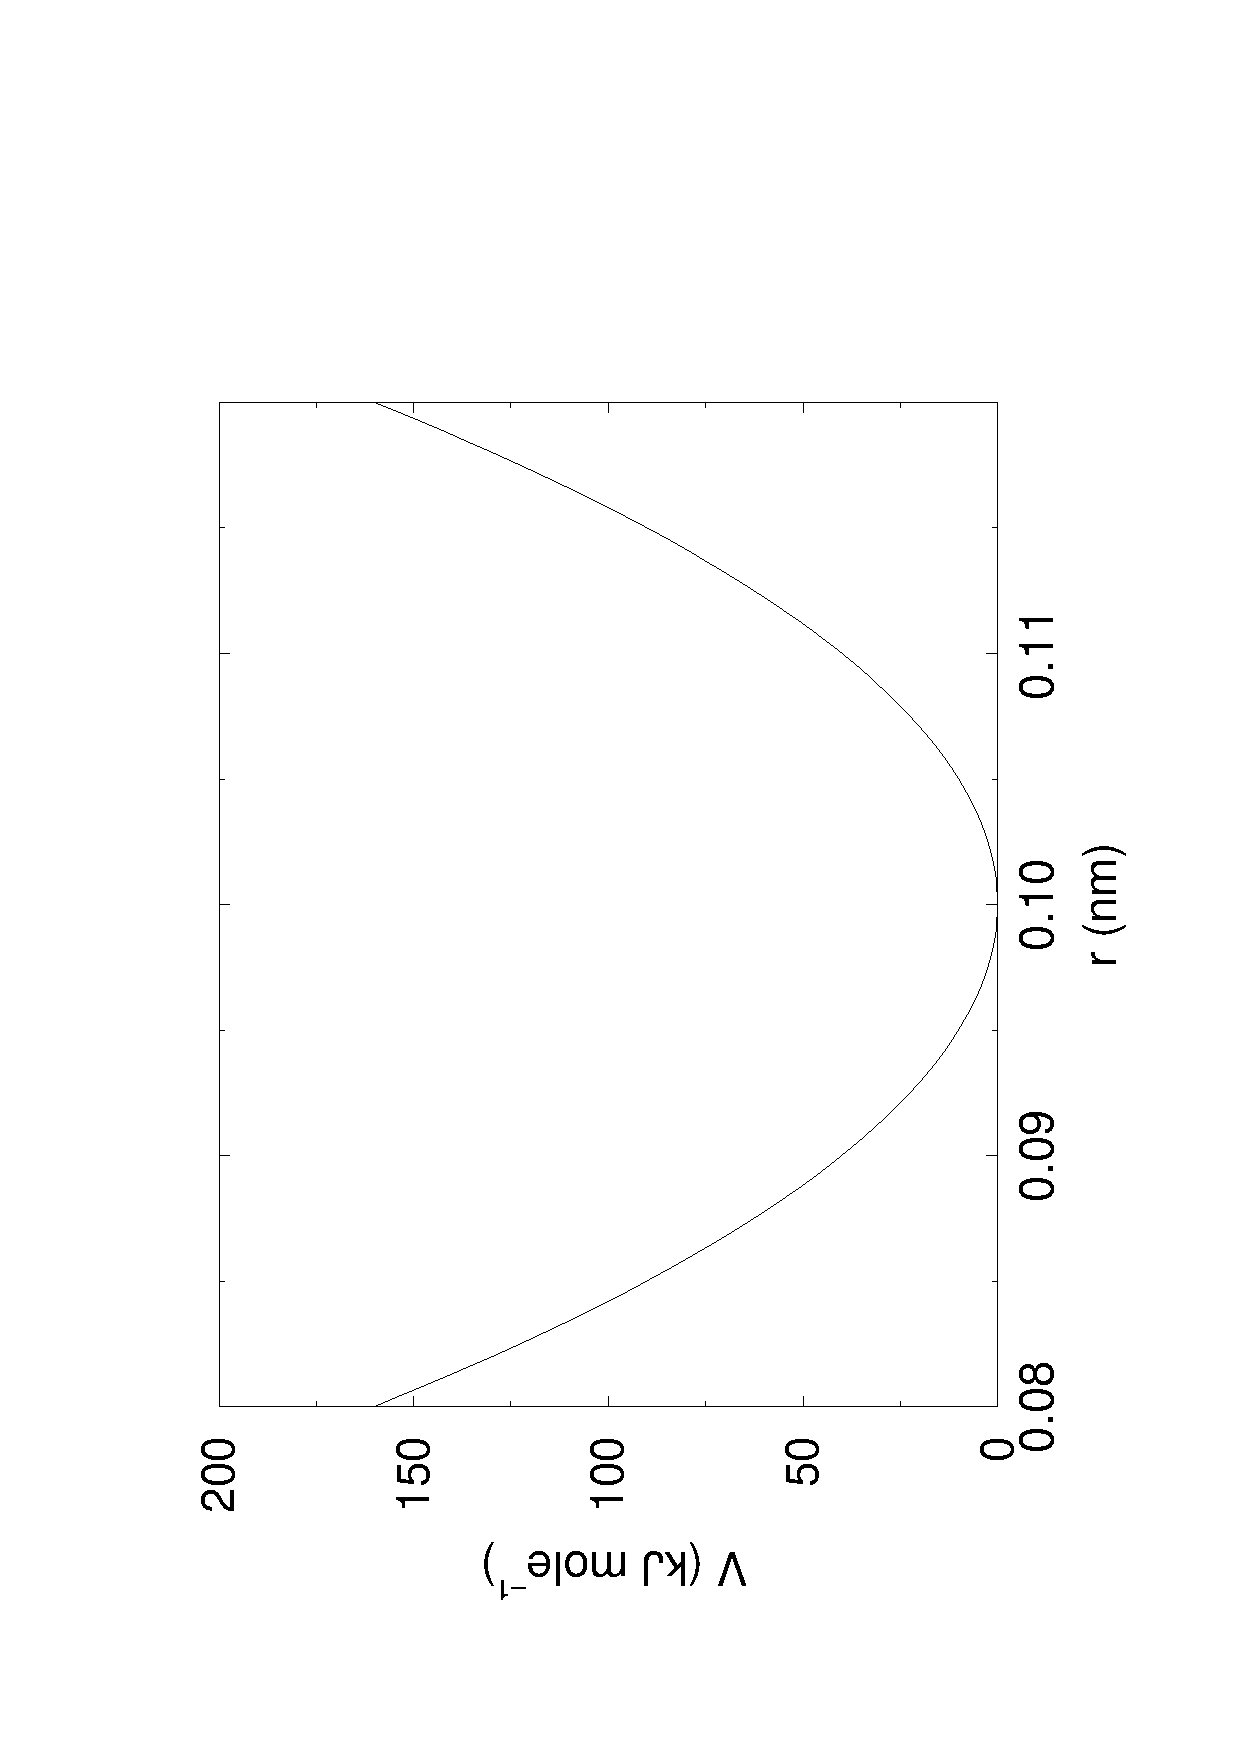
\includegraphics[width=7cm]{plots/f-bond}}
\caption[Bond stretching.]{Principle of bond stretching (left), and the bond
stretching potential (right).}
\label{fig:bstretch1}
\end{figure}

\beq
V_b~(\rij) = \half k^b_{ij}(\rij-b_{ij})^2
\eeq
See also \figref{bstretch1}, with the force given by:
\beq
\ve{F}_i(\rvij) = k^b_{ij}(\rij-b_{ij}) \rnorm
\eeq

%\ifthenelse{\equal{\gmxlite}{1}}{}{
\subsubsection{Fourth power potential}
\label{subsec:G96bond}
In the \gromosv{96} force field~\cite{gromos96}, the covalent bond potential
is, for reasons of computational efficiency, written as:
\beq
V_b~(\rij) = \frac{1}{4}k^b_{ij}\left(\rij^2-b_{ij}^2\right)^2
\eeq
The corresponding force is:
\beq
\ve{F}_i(\rvij) = k^b_{ij}(\rij^2-b_{ij}^2)~\rvij
\eeq
The force constants for this form of the potential are related to the usual
harmonic force constant $k^{b,\mathrm{harm}}$ (\secref{bondpot}) as
\beq
2 k^b b_{ij}^2 = k^{b,\mathrm{harm}}
\eeq
The force constants are mostly derived from the harmonic ones used in 
\gromosv{87}~\cite{biomos}. Although this form is computationally more 
efficient
(because no square root has to be evaluated), it is conceptually more
complex. One particular disadvantage is that since the form is not harmonic,
the average energy of a single bond is not equal to $\half kT$ as it is for 
the normal harmonic potential.

\subsection{\normindex{Morse potential} bond stretching}
\label{subsec:Morsebond}
%\author{F.P.X. Everdij}
%
For some systems that require an anharmonic bond stretching potential,
the Morse potential~\cite{Morse29} 
between two atoms {\it i} and {\it j} is available
in {\gromacs}. This potential differs from the harmonic potential in 
that it has an asymmetric potential well and a zero force at infinite
distance. The functional form is:
\beq
\displaystyle V_{morse} (r_{ij}) = D_{ij} [1 - \exp(-\beta_{ij}(r_{ij}-b_{ij}))]^2,
\eeq
See also \figref{morse}, and the corresponding force is:
\beq
\begin{array}{rcl}
\displaystyle {\bf F}_{morse} ({\bf r}_{ij})&=&2 D_{ij} \beta_{ij} \exp(-\beta_{ij}(r_{ij}-b_{ij})) * \\
\displaystyle \: & \: &[1 - \exp(-\beta_{ij}(r_{ij}-b_{ij}))] \frac{\displaystyle {\bf r}_{ij}}{\displaystyle r_{ij}},
\end{array}
\eeq
where \( \displaystyle D_{ij} \) is the depth of the well in kJ/mol,
\( \displaystyle \beta_{ij} \) defines the steepness of the well (in
nm\(^{-1} \)), and \( \displaystyle b_{ij} \) is the equilibrium
distance in nm.  The steepness parameter \( \displaystyle \beta_{ij}
\) can be expressed in terms of the reduced mass of the atoms {\it i}
and {\it j}, the fundamental vibration frequency \( \displaystyle
\omega_{ij} \) and the well depth \( \displaystyle D_{ij} \):
\beq
\displaystyle \beta_{ij}= \omega_{ij} \sqrt{\frac{\mu_{ij}}{2 D_{ij}}}
\eeq
and because \( \displaystyle \omega = \sqrt{k/\mu} \), one can rewrite \( \displaystyle \beta_{ij} \) in terms of the harmonic force constant \( \displaystyle k_{ij} \):
\beq
\displaystyle \beta_{ij}= \sqrt{\frac{k_{ij}}{2 D_{ij}}}
\label{eqn:betaij}
\eeq
For small deviations \( \displaystyle (r_{ij}-b_{ij}) \), one can
approximate the \( \displaystyle \exp \)-term to first-order using a
Taylor expansion:
\beq
\displaystyle \exp(-x) \approx 1-x
\label{eqn:expminx}
\eeq
and substituting \eqnref{betaij} and \eqnref{expminx} in the functional form:
\beq
\begin{array}{rcl}
\displaystyle V_{morse} (r_{ij})&=&D_{ij} [1 - \exp(-\beta_{ij}(r_{ij}-b_{ij}))]^2\\
\displaystyle \:&=&D_{ij} [1 - (1 -\sqrt{\frac{k_{ij}}{2 D_{ij}}}(r_{ij}-b_{ij}))]^2\\
\displaystyle \:&=&\frac{1}{2} k_{ij} (r_{ij}-b_{ij}))^2
\end{array}
\eeq
we recover the harmonic bond stretching potential.

\begin{figure}
\centerline{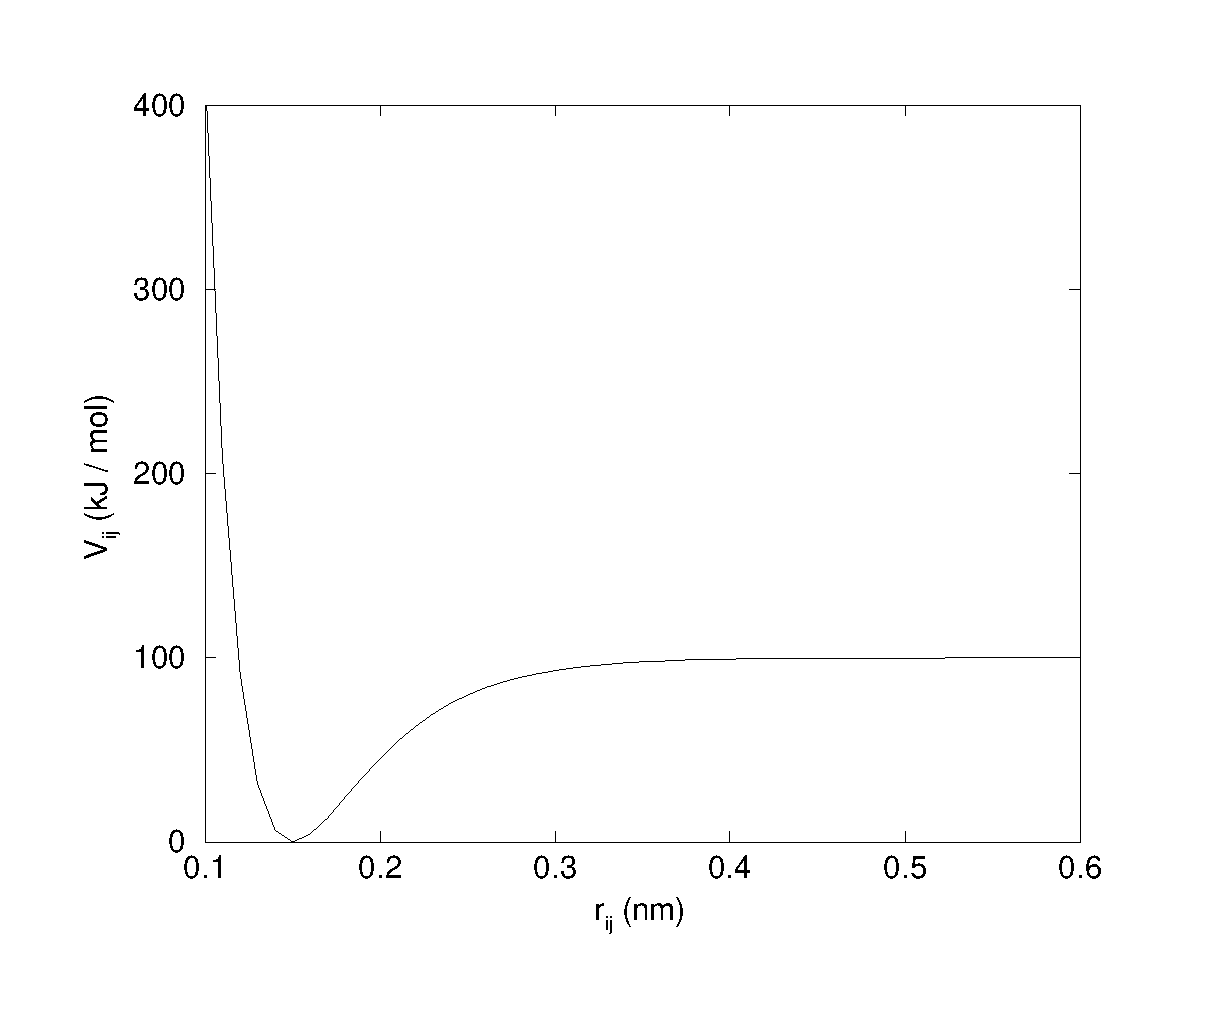
\includegraphics[width=7cm]{plots/f-morse}}
\caption{The Morse potential well, with bond length 0.15 nm.}
\label{fig:morse}
\end{figure}

\subsection{Cubic bond stretching potential}
\label{subsec:cubicbond}
Another anharmonic bond stretching potential that is slightly simpler
than the Morse potential adds a cubic term in the distance to the
simple harmonic form:
\beq
V_b~(\rij) = k^b_{ij}(\rij-b_{ij})^2 + k^b_{ij}k^{cub}_{ij}(\rij-b_{ij})^3
\eeq
A flexible \normindex{water} model (based on
the SPC water model~\cite{Berendsen81}) including 
a cubic bond stretching potential for the O-H bond
was developed by Ferguson~\cite{Ferguson95}. This model was found
to yield a reasonable infrared spectrum. The Ferguson water model is
available in the {\gromacs} library ({\tt flexwat-ferguson.itp}). 
It should be noted that the potential is asymmetric: overstretching leads to
infinitely low energies. The \swapindex{integration}{timestep} is therefore
limited to 1 fs.

The force corresponding to this potential is:
\beq
\ve{F}_i(\rvij) = 2k^b_{ij}(\rij-b_{ij})~\rnorm + 3k^b_{ij}k^{cub}_{ij}(\rij-b_{ij})^2~\rnorm
\eeq

\subsection{FENE bond stretching potential\index{FENE potential}}
\label{subsec:FENEbond}
In coarse-grained polymer simulations the beads are often connected
by a FENE (finitely extensible nonlinear elastic) potential~\cite{Warner72}:
\beq
V_{\mbox{\small FENE}}(\rij) =
  -\half k^b_{ij} b^2_{ij} \log\left(1 - \frac{\rij^2}{b^2_{ij}}\right)
\eeq
The potential looks complicated, but the expression for the force is simpler:
\beq
F_{\mbox{\small FENE}}(\rvij) =
  -k^b_{ij} \left(1 - \frac{\rij^2}{b^2_{ij}}\right)^{-1} \rvij
\eeq
At short distances the potential asymptotically goes to a harmonic
potential with force constant $k^b$, while it diverges at distance $b$.
%} % Brace matches ifthenelse test for gmxlite

\subsection{Harmonic angle potential}
\label{subsec:harmonicangle}
\newcommand{\tijk}{\theta_{ijk}}
The bond-\swapindex{angle}{vibration} between a triplet of atoms $i$ - $j$ - $k$
is also represented by a harmonic potential on the angle $\tijk$

\begin{figure}
\centerline{\raisebox{1cm}{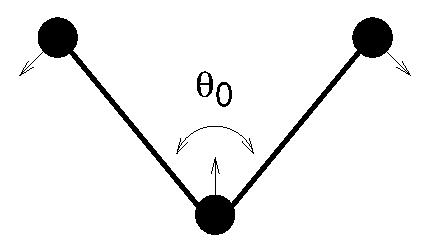
\includegraphics[width=5cm]{plots/angle}}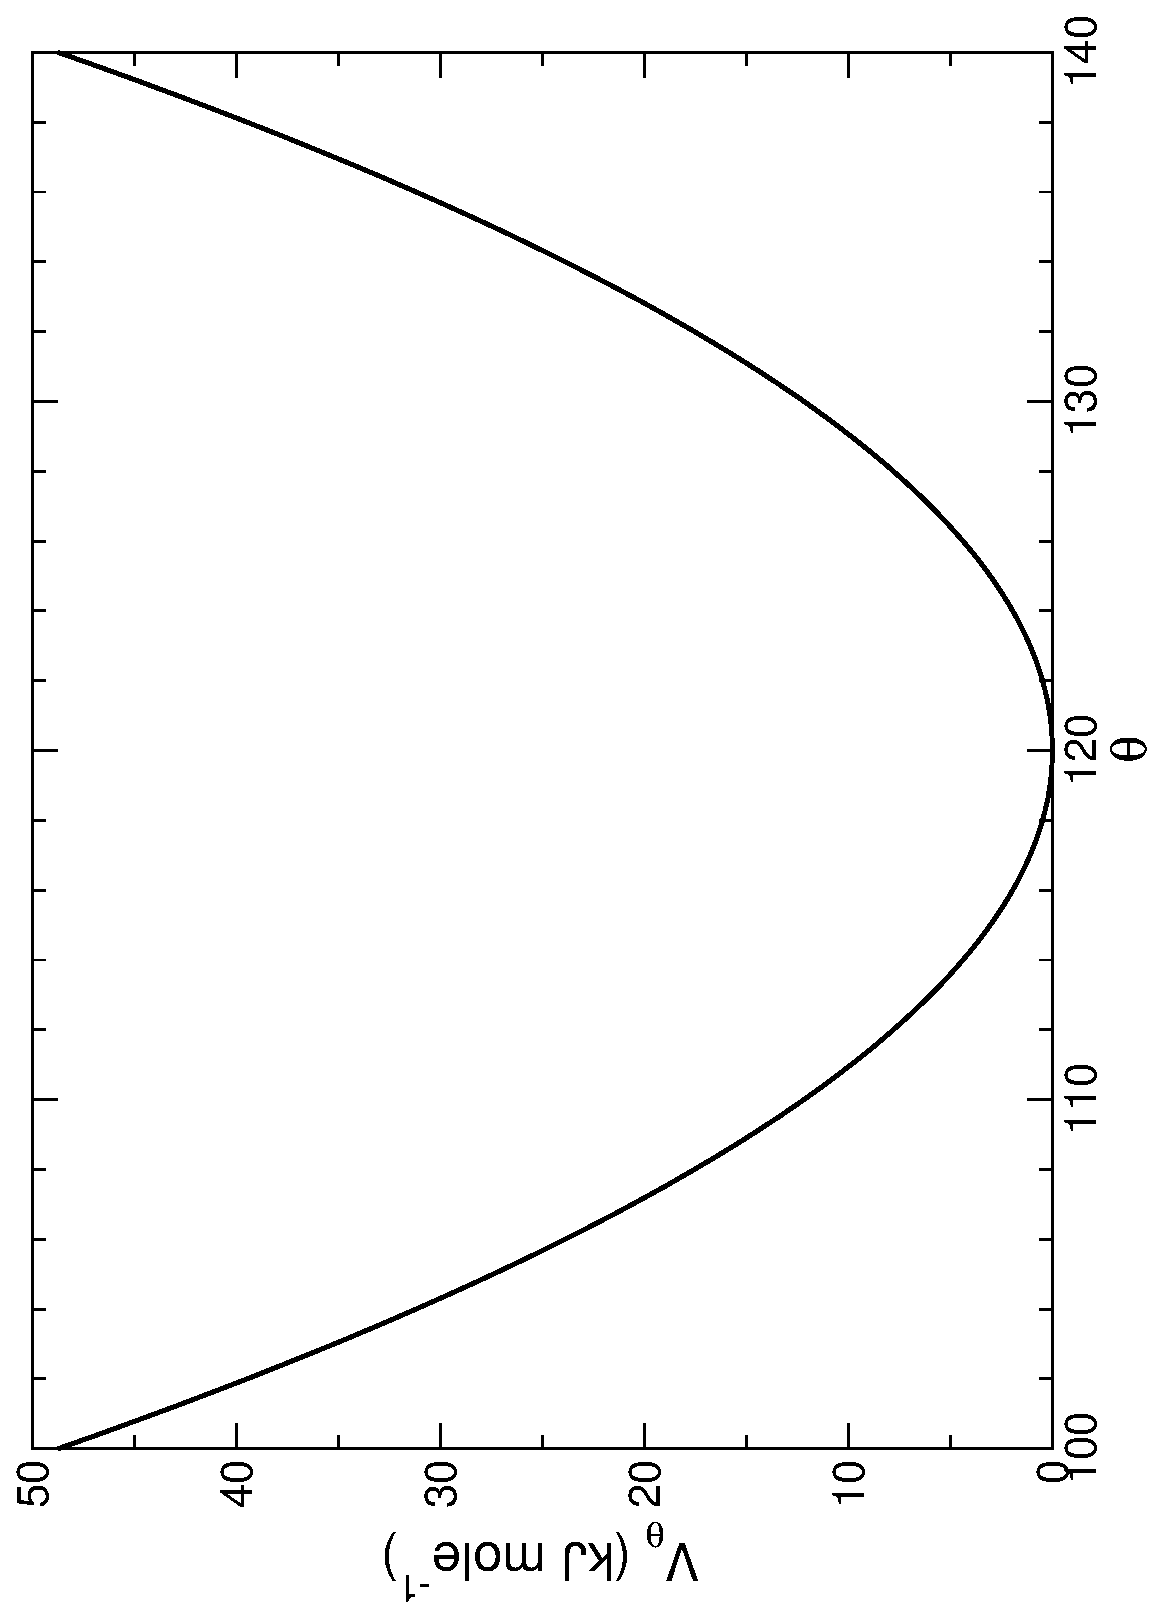
\includegraphics[width=7cm]{plots/f-angle}}
\caption[Angle vibration.]{Principle of angle vibration (left) and the
bond angle potential (right).}
\label{fig:angle}
\end{figure}

\beq
V_a(\tijk) = \half k^{\theta}_{ijk}(\tijk-\tijk^0)^2
\eeq
As the bond-angle vibration is represented by a harmonic potential, the
form is the same as the bond stretching (\figref{bstretch1}).

The force equations are given by the chain rule:
\beq
\begin{array}{l}
\Fvi    ~=~ -\displaystyle\frac{d V_a(\tijk)}{d \rvi}   \\
\Fvk    ~=~ -\displaystyle\frac{d V_a(\tijk)}{d \rvk}   \\
\Fvj    ~=~ -\Fvi-\Fvk
\end{array}
~ \mbox{ ~ where ~ } ~
 \tijk = \arccos \frac{(\rvij \cdot \ve{r}_{kj})}{r_{ij}r_{kj}}
\eeq
The numbering $i,j,k$ is in sequence of covalently bonded atoms. Atom
$j$ is in the middle; atoms $i$  and $k$ are at the ends (see \figref{angle}).
{\bf Note} that in the input in topology files, angles are given in degrees and
force constants in kJ/mol/rad$^2$.

%\ifthenelse{\equal{\gmxlite}{1}}{}{
\subsection{Cosine based angle potential}
\label{subsec:G96angle}
In the \gromosv{96} force field a simplified function is used to represent angle
vibrations:
\beq
V_a(\tijk) = \half k^{\theta}_{ijk}\left(\cos(\tijk) - \cos(\tijk^0)\right)^2
\label{eq:G96angle}
\eeq
where 
\beq
\cos(\tijk) = \frac{\rvij\cdot\ve{r}_{kj}}{\rij r_{kj}}
\eeq
The corresponding force can be derived by partial differentiation with respect
to the atomic positions. The force constants in this function are related
to the force constants in the harmonic form $k^{\theta,\mathrm{harm}}$
(\ssecref{harmonicangle}) by:
\beq
k^{\theta} \sin^2(\tijk^0) = k^{\theta,\mathrm{harm}}
\eeq
In the \gromosv{96} manual there is a much more complicated conversion formula
which is temperature dependent. The formulas are equivalent at 0 K
and the differences at 300 K are on the order of 0.1 to 0.2\%.
{\bf Note} that in the input in topology files, angles are given in degrees and
force constants in kJ/mol.

\subsection{Restricted bending potential}
\label{subsec:ReB}
The restricted bending (ReB) potential~\cite{MonicaGoga2013} prevents the bending angle $\theta$
from reaching the $180^{\circ}$ value. In this way, the numerical instabilities
due to the calculation of the torsion angle and potential are eliminated when
performing coarse-grained molecular dynamics simulations.

To systematically hinder the bending angles from reaching the $180^{\circ}$ value,
the bending potential \ref{eq:G96angle} is divided by a $\sin^2\theta$ factor:
%
\beq
V_{\rm ReB}(\theta_i) = \frac{1}{2} k_{\theta} \frac{(\cos\theta_i - \cos\theta_0)^2}{\sin^2\theta_i}.
\label{eq:ReB}
\eeq
%
Figure ~\figref{ReB} shows the comparison between the ReB potential, \ref{eq:ReB},
and the standard one \ref{eq:G96angle}.
%
\begin{figure}
\centerline{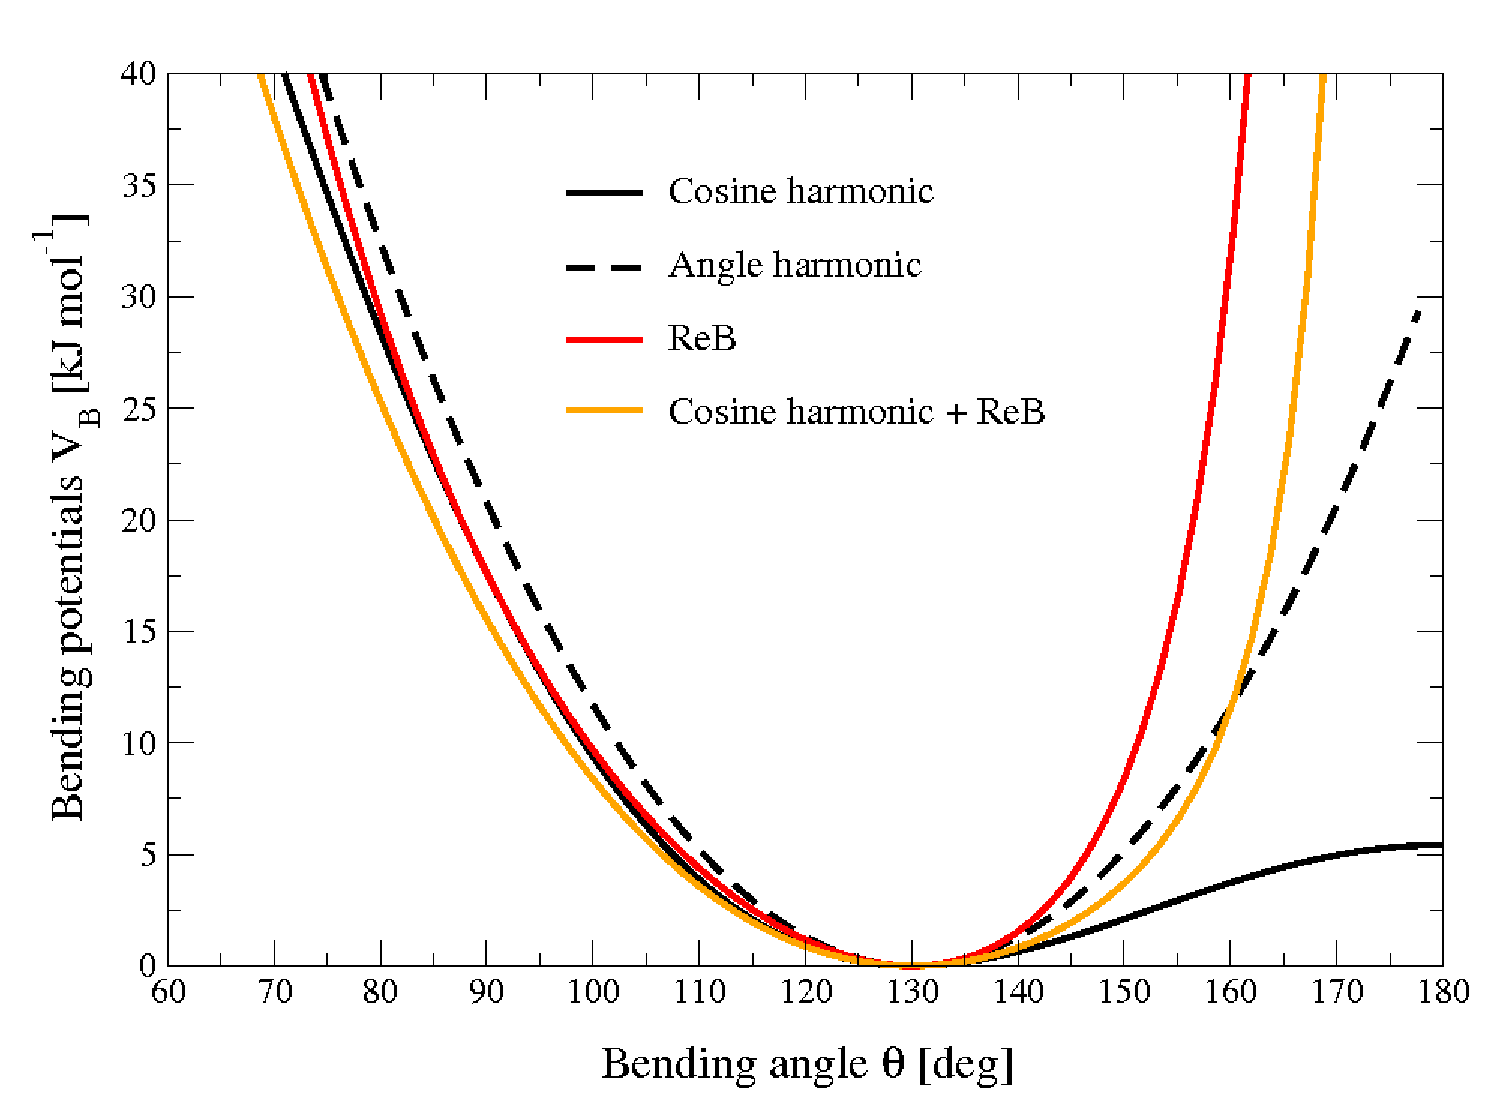
\includegraphics[width=10cm]{plots/fig-02}}
\vspace*{8pt}
\caption{Bending angle potentials: cosine harmonic (solid black line), angle harmonic
(dashed black line) and restricted bending (red) with the same bending constant
$k_{\theta}=85$ kJ mol$^{-1}$ and equilibrium angle $\theta_0=130^{\circ}$.
The orange line represents the sum of a cosine harmonic ($k =50$ kJ mol$^{-1}$)
with a restricted bending ($k =25$ kJ mol$^{-1}$) potential, both with $\theta_0=130^{\circ}$.}
\label{fig:ReB}
\end{figure}
%
The wall of the ReB potential is very repulsive in the region close to $180^{\circ}$ and,
as a result, the bending angles are kept within a safe interval, far from instabilities.
The power $2$ of $\sin\theta_i$ in the denominator has been chosen to guarantee this behavior
and allows an elegant differentiation:
%
\beq
F_{\rm ReB}(\theta_i) = \frac{2k_{\theta}}{\sin^4\theta_i}(\cos\theta_i - \cos\theta_0) (1 - \cos\theta_i\cos\theta_0) \frac{\partial \cos\theta_i}{\partial \vec r_{k}}.
\label{eq:diff_ReB}
\eeq
%
Due to its construction, the restricted bending potential cannot be used for equilibrium
$\theta_0$ values too close to $0^{\circ}$ or $180^{\circ}$ (from experience, at least $10^{\circ}$
difference is recommended). It is very important that, in the starting configuration,
all the bending angles have to be in the safe interval to avoid initial instabilities.
This bending potential can be used in combination with any form of torsion potential.
It will always prevent three consecutive particles from becoming collinear and,
as a result, any torsion potential will remain free of singularities.
It can be also added to a standard bending potential to affect the angle around $180^{\circ}$,
but to keep its original form around the minimum (see the orange curve in \figref{ReB}).


\subsection{Urey-Bradley potential}
\label{subsec:Urey-Bradley}
The \swapindex{Urey-Bradley bond-angle}{vibration} between a triplet
of atoms $i$ - $j$ - $k$ is represented by a harmonic potential on the
angle $\tijk$ and a harmonic correction term on the distance between
the atoms $i$ and $k$. Although this can be easily written as a simple
sum of two terms, it is convenient to have it as a single entry in the
topology file and in the output as a separate energy term. It is used mainly
in the CHARMm force field~\cite{BBrooks83}. The energy is given by:

\beq
V_a(\tijk) = \half k^{\theta}_{ijk}(\tijk-\tijk^0)^2 + \half k^{UB}_{ijk}(r_{ik}-r_{ik}^0)^2
\eeq

The force equations can be deduced from sections~\ssecref{harmonicbond}
and~\ssecref{harmonicangle}.

\subsection{Bond-Bond cross term}
\label{subsec:bondbondcross}
The bond-bond cross term for three particles $i, j, k$ forming bonds
$i-j$ and $k-j$ is given by~\cite{Lawrence2003b}:
\begin{equation}
V_{rr'} ~=~ k_{rr'} \left(\left|\ve{r}_{i}-\ve{r}_j\right|-r_{1e}\right) \left(\left|\ve{r}_{k}-\ve{r}_j\right|-r_{2e}\right)
\label{crossbb}
\end{equation}
where $k_{rr'}$ is the force constant, and $r_{1e}$ and $r_{2e}$ are the
equilibrium bond lengths of the $i-j$ and $k-j$ bonds respectively. The force
associated with this potential on particle $i$ is:
\begin{equation}
\ve{F}_{i} = -k_{rr'}\left(\left|\ve{r}_{k}-\ve{r}_j\right|-r_{2e}\right)\frac{\ve{r}_i-\ve{r}_j}{\left|\ve{r}_{i}-\ve{r}_j\right|}
\end{equation}
The force on atom $k$ can be obtained by swapping $i$ and $k$ in the above
equation. Finally, the force on atom $j$ follows from the fact that the sum
of internal forces should be zero: $\ve{F}_j = -\ve{F}_i-\ve{F}_k$.

\subsection{Bond-Angle cross term}
\label{subsec:bondanglecross}
The bond-angle cross term for three particles $i, j, k$ forming bonds
$i-j$ and $k-j$ is given by~\cite{Lawrence2003b}:
\begin{equation}
V_{r\theta} ~=~ k_{r\theta} \left(\left|\ve{r}_{i}-\ve{r}_k\right|-r_{3e} \right) \left(\left|\ve{r}_{i}-\ve{r}_j\right|-r_{1e} + \left|\ve{r}_{k}-\ve{r}_j\right|-r_{2e}\right)
\end{equation}
where $k_{r\theta}$ is the force constant, $r_{3e}$ is the $i-k$ distance,
and the other constants are the same as in Equation~\ref{crossbb}. The force
associated with the potential on atom $i$ is:
\begin{equation}
\ve{F}_{i} ~=~ -k_{r\theta}\left[\left(\left|\ve{r}_{i}-\ve{r}_{k}\right|-r_{3e}\right)\frac{\ve{r}_i-\ve{r}_j}{\left|\ve{r}_{i}-\ve{r}_j\right|} \\
+ \left(\left|\ve{r}_{i}-\ve{r}_j\right|-r_{1e} + \left|\ve{r}_{k}-\ve{r}_j\right|-r_{2e}\right)\frac{\ve{r}_i-\ve{r}_k}{\left|\ve{r}_{i}-\ve{r}_k\right|}\right]
\end{equation}

\subsection{Quartic angle potential}
\label{subsec:quarticangle}
For special purposes there is an angle potential
that uses a fourth order polynomial:
\beq
V_q(\tijk) ~=~ \sum_{n=0}^5 C_n (\tijk-\tijk^0)^n
\eeq
%} % Brace matches ifthenelse test for gmxlite

%% new commands %%%%%%%%%%%%%%%%%%%%%%
\newcommand{\rvkj}{{\bf r}_{kj}}
\newcommand{\rkj}{r_{kj}}
%%%%%%%%%%%%%%%%%%%%%%%%%%%%%%%%%%%%%%

\subsection{Improper dihedrals\swapindexquiet{improper}{dihedral}}
\label{sec:imp}
Improper dihedrals are meant to keep \swapindex{planar}{group}s ({\eg} 
aromatic rings) planar, or to prevent molecules from flipping over to their
\normindex{mirror image}s, see \figref{imp}.

\begin {figure}
\centerline{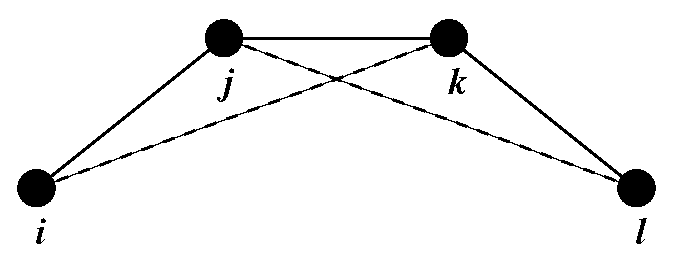
\includegraphics[width=4cm]{plots/ring-imp}\hspace{1cm}
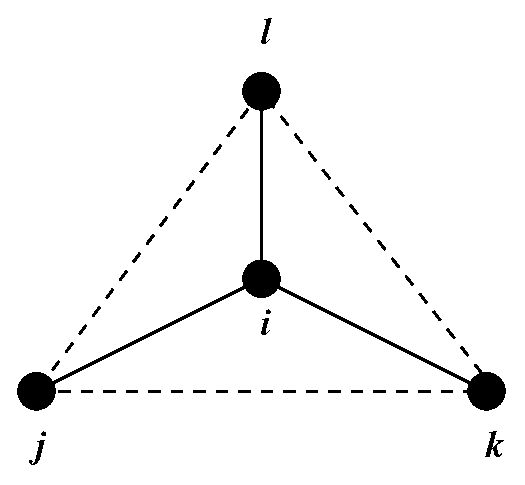
\includegraphics[width=3cm]{plots/subst-im}\hspace{1cm}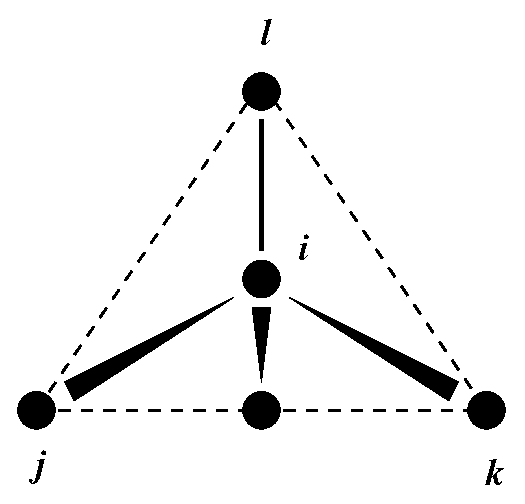
\includegraphics[width=3cm]{plots/tetra-im}}
\caption[Improper dihedral angles.]{Principle of improper
dihedral angles. Out of plane bending for rings (left), substituents
of rings (middle), out of tetrahedral (right). The improper dihedral
angle $\xi$ is defined as the angle between planes (i,j,k) and (j,k,l)
in all cases.}
\label{fig:imp}
\end {figure}

\subsubsection{Improper dihedrals: harmonic type}
\label{subsec:harmonicimproperdihedral}
The simplest improper dihedral potential is a harmonic potential; it is plotted in
\figref{imps}.
\beq
V_{id}(\xi_{ijkl}) = \half k_{\xi}(\xi_{ijkl}-\xi_0)^2
\eeq
Since the potential is harmonic it is discontinuous,
but since the discontinuity is chosen at 180$^\circ$ distance from $\xi_0$
this will never cause problems.
{\bf Note} that in the input in topology files, angles are given in degrees and
force constants in kJ/mol/rad$^2$.

\begin{figure}
\centerline{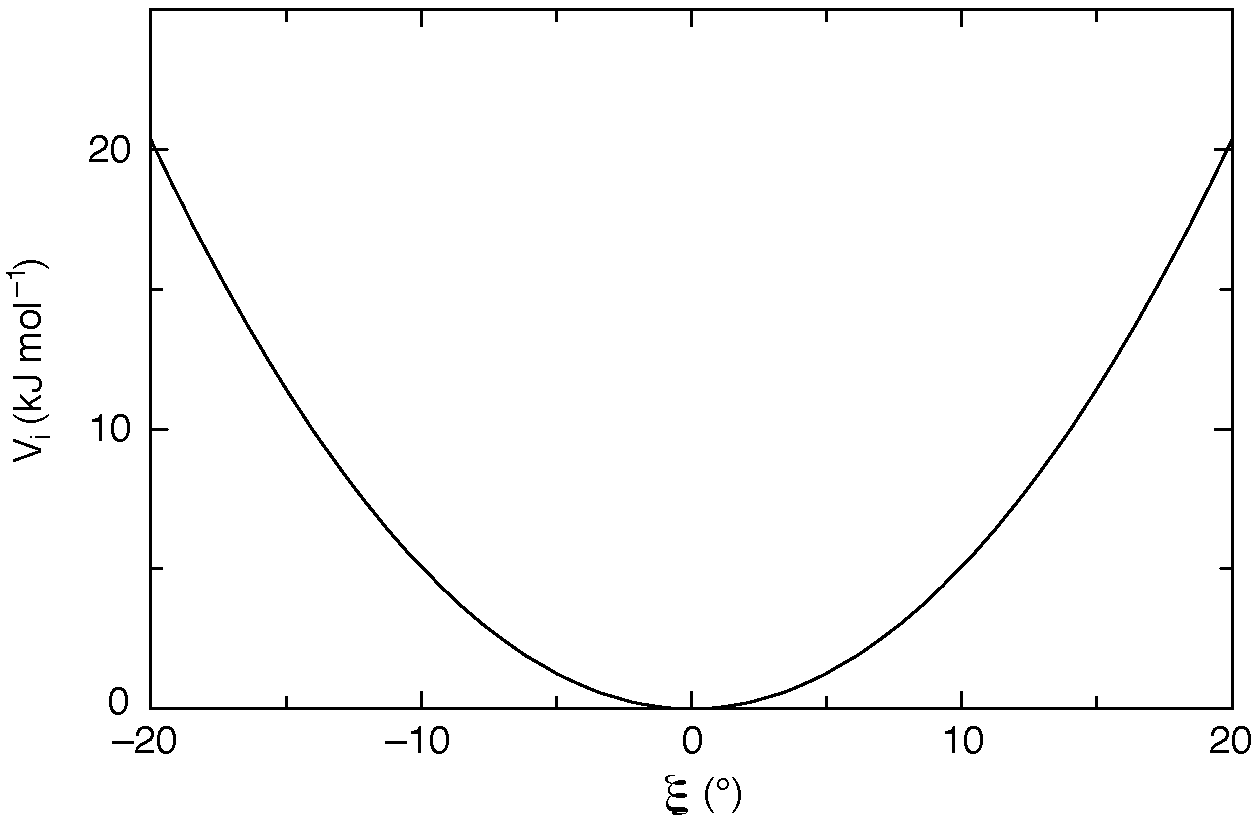
\includegraphics[width=10cm]{plots/f-imps.pdf}}
\caption{Improper dihedral potential.}
\label{fig:imps}
\end{figure}

\subsubsection{Improper dihedrals: periodic type}
\label{subsec:periodicimproperdihedral}
This potential is identical to the periodic proper dihedral (see below).
There is a separate dihedral type for this (type 4) only to be able
to distinguish improper from proper dihedrals in the parameter section
and the output.

\subsection{Proper dihedrals\swapindexquiet{proper}{dihedral}}
For the normal \normindex{dihedral} interaction there is a choice of
either the {\gromos} periodic function or a function based on
expansion in powers of $\cos \phi$ (the so-called Ryckaert-Bellemans
potential). This choice has consequences for the inclusion of special
interactions between the first and the fourth atom of the dihedral
quadruple. With the periodic {\gromos} potential a special 1-4
LJ-interaction must be included; with the Ryckaert-Bellemans potential
{\em for alkanes} the \normindex{1-4 interaction}s must be excluded
from the non-bonded list.  {\bf Note:} Ryckaert-Bellemans potentials
are also used in {\eg} the OPLS force field in combination with 1-4
interactions. You should therefore not modify topologies generated by
{\tt \normindex{pdb2gmx}} in this case.

\subsubsection{Proper dihedrals: periodic type}
\label{subsec:properdihedral}
Proper dihedral angles are defined according to the IUPAC/IUB
convention, where $\phi$ is the angle between the $ijk$ and the $jkl$
planes, with {\bf zero} corresponding to the {\em cis} configuration
($i$ and $l$ on the same side). There are two dihedral function types
in {\gromacs} topology files. There is the standard type 1 which behaves
like any other bonded interactions. For certain force fields, type 9
is useful. Type 9 allows multiple potential functions to be applied
automatically to a single dihedral in the {\tt [ dihedral ]} section
when multiple parameters are defined for the same atomtypes
in the {\tt [ dihedraltypes ]} section.

\begin{figure}
\centerline{\raisebox{1cm}{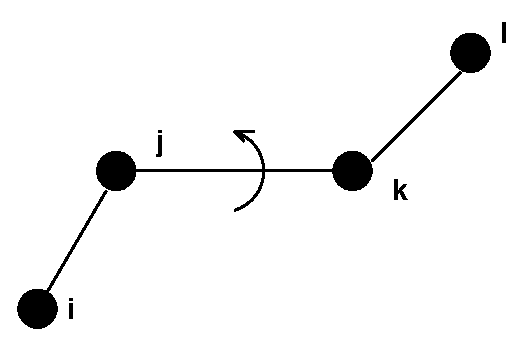
\includegraphics[width=5cm]{plots/dih}}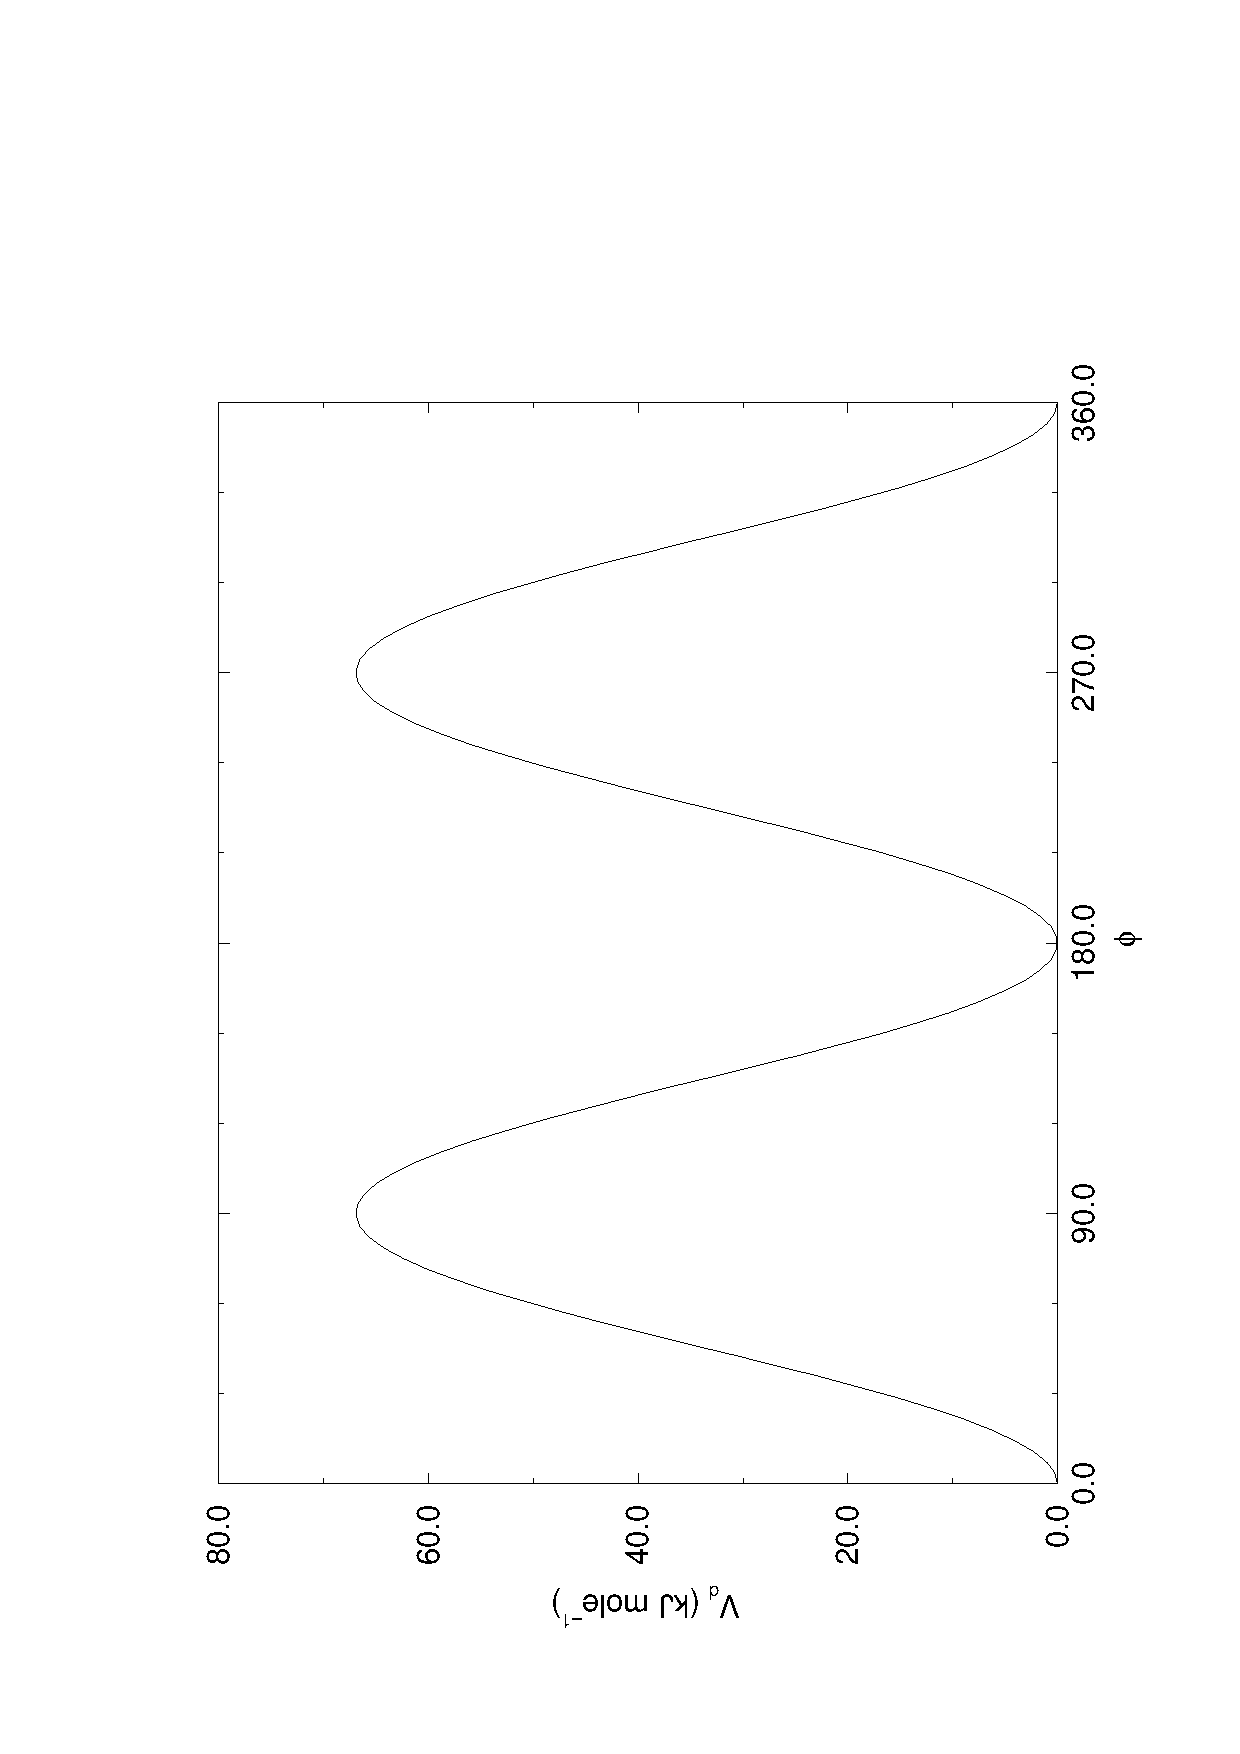
\includegraphics[width=7cm]{plots/f-dih}}
\caption[Proper dihedral angle.]{Principle of proper dihedral angle
(left, in {\em trans} form) and the dihedral angle potential (right).} 
\label{fig:pdihf}
\end{figure}
\beq
V_d(\phi_{ijkl}) = k_{\phi}(1 + \cos(n \phi - \phi_s))
\eeq

%\ifthenelse{\equal{\gmxlite}{1}}{}{
\subsubsection{Proper dihedrals: Ryckaert-Bellemans function}
\label{subsec:RBdihedral}
For alkanes, the following proper dihedral potential is often used
(see \figref{rbdih}):
\beq
V_{rb}(\phi_{ijkl}) = \sum_{n=0}^5 C_n( \cos(\psi ))^n,
\eeq 
where $\psi = \phi - 180^\circ$.  \\
{\bf Note:} A conversion from one convention to another can be achieved by 
multiplying every coefficient \( \displaystyle C_n \) 
by \( \displaystyle (-1)^n \).

An example of constants for $C$ is given in \tabref{crb}.

\begin{table}
\centerline{
\begin{tabular}{|lr|lr|lr|}
\dline
$C_0$   & 9.28  & $C_2$   & -13.12  & $C_4$   & 26.24   \\
$C_1$   & 12.16 & $C_3$   & -3.06   & $C_5$   & -31.5   \\
\dline
\end{tabular}
}
\caption{Constants for Ryckaert-Bellemans potential (kJ mol$^{-1}$).}
\label{tab:crb}
\end{table}

\begin{figure}
\centerline{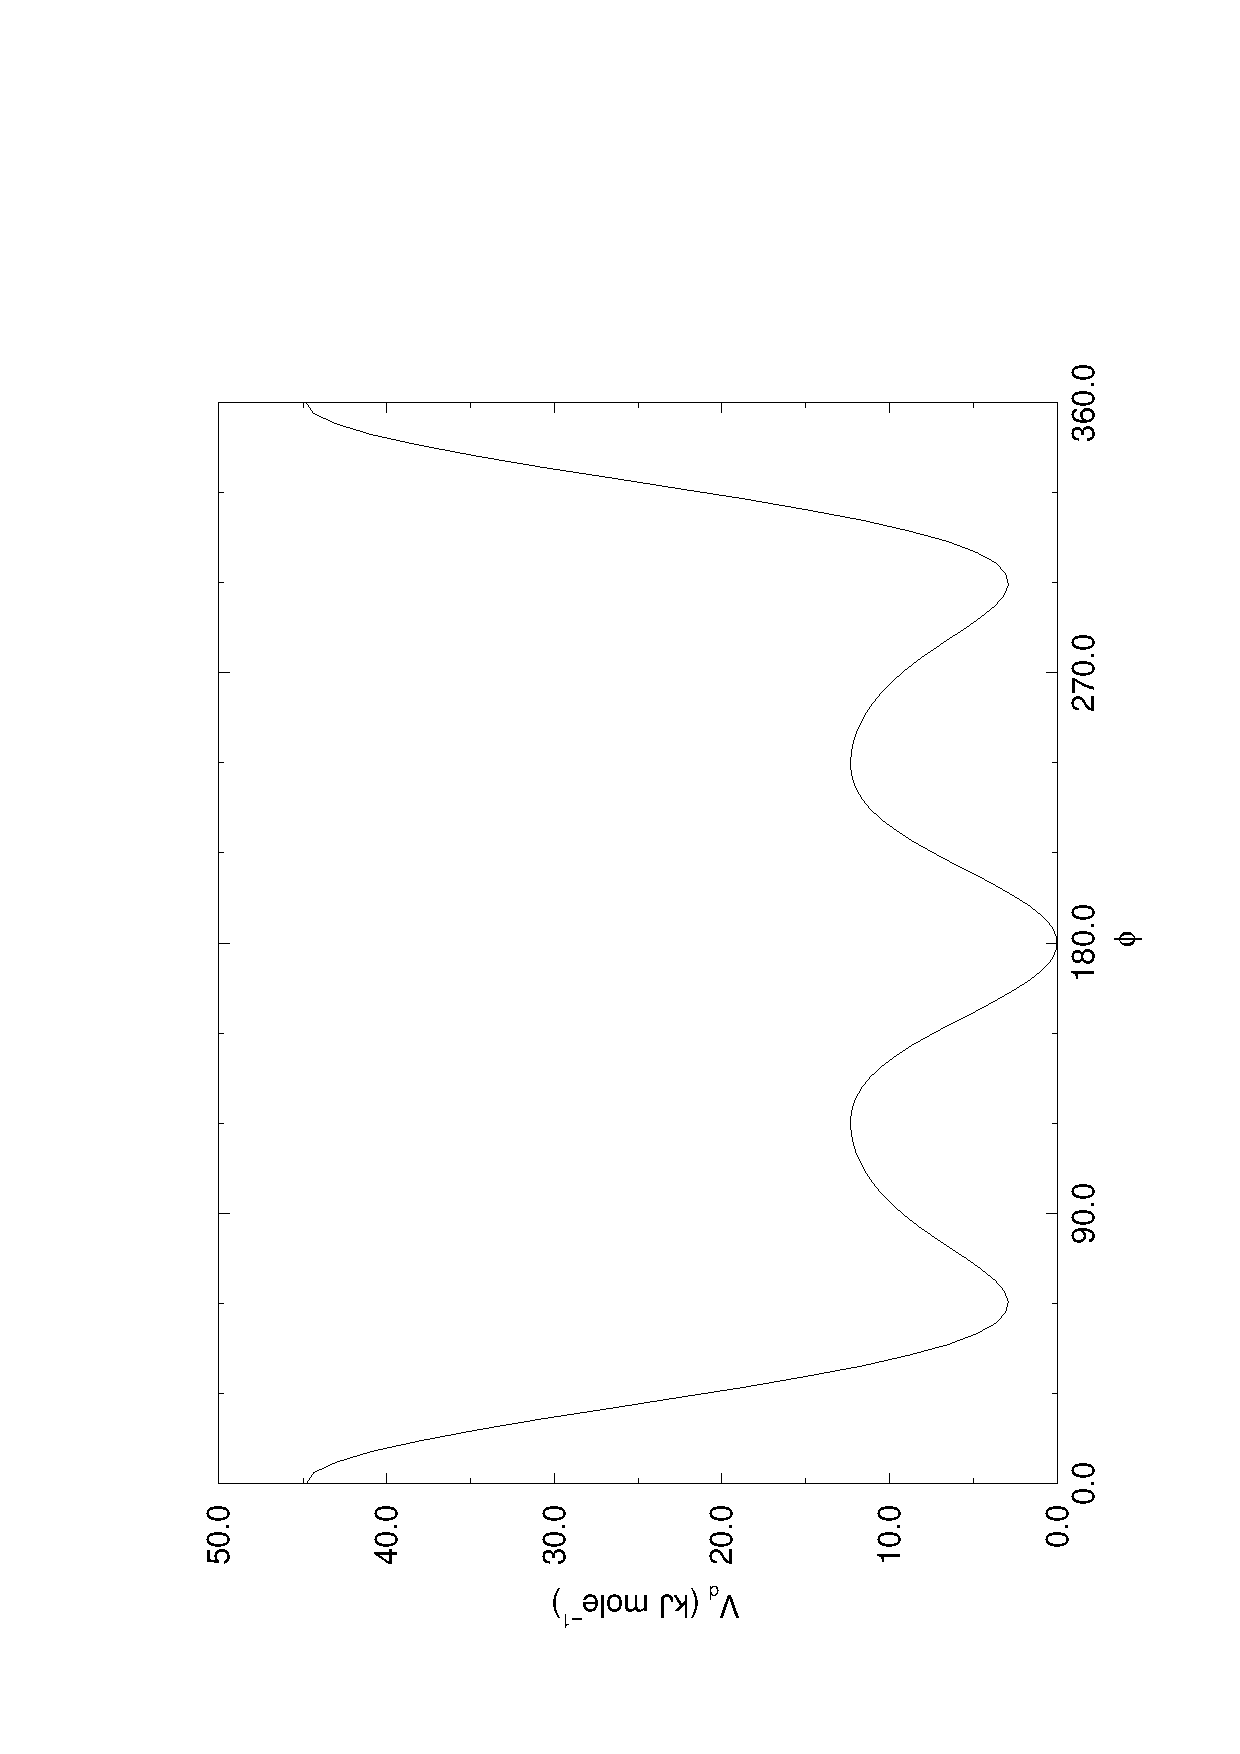
\includegraphics[width=8cm]{plots/f-rbs}}
\caption{Ryckaert-Bellemans dihedral potential.}
\label{fig:rbdih}
\end{figure}

({\bf Note:} The use of this potential implies exclusion of LJ interactions
between the first and the last atom of the dihedral, and $\psi$ is defined
according to the ``polymer convention'' ($\psi_{trans}=0$).)

The RB dihedral function can also be used to include Fourier dihedrals
(see below):
\beq
V_{rb} (\phi_{ijkl}) ~=~ \frac{1}{2} \left[F_1(1+\cos(\phi)) + F_2(
1-\cos(2\phi)) + F_3(1+\cos(3\phi)) + F_4(1-\cos(4\phi))\right]
\eeq
Because of the equalities \( \cos(2\phi) = 2\cos^2(\phi) - 1 \),
\( \cos(3\phi) = 4\cos^3(\phi) - 3\cos(\phi) \) and
\( \cos(4\phi) = 8\cos^4(\phi) - 8\cos^2(\phi) + 1 \)
one can translate the OPLS parameters to 
Ryckaert-Bellemans parameters as follows:
\beq
\displaystyle
\begin{array}{rcl}
\displaystyle C_0&=&F_2 + \frac{1}{2} (F_1 + F_3)\\
\displaystyle C_1&=&\frac{1}{2} (- F_1 + 3 \, F_3)\\
\displaystyle C_2&=& -F_2 + 4 \, F_4\\
\displaystyle C_3&=&-2 \, F_3\\
\displaystyle C_4&=&-4 \, F_4\\
\displaystyle C_5&=&0
\end{array}
\eeq 
with OPLS parameters in protein convention and RB parameters in
polymer convention (this yields a minus sign for the odd powers of 
cos$(\phi)$).\\
\noindent{\bf Note:} Mind the conversion from {\bf kcal mol$^{-1}$} for 
literature OPLS and RB parameters to {\bf kJ mol$^{-1}$} in {\gromacs}.\\
%} % Brace matches ifthenelse test for gmxlite

\subsubsection{Proper dihedrals: Fourier function}
\label{subsec:Fourierdihedral}
The OPLS potential function is given as the first three
or four~\cite{Jorgensen2005a} cosine terms of a Fourier series.
In {\gromacs} the four term function is implemented:
\beq
V_{F} (\phi_{ijkl}) ~=~ \frac{1}{2} \left[C_1(1+\cos(\phi)) + C_2(
1-\cos(2\phi)) + C_3(1+\cos(3\phi)) + C_4(1-\cos(4\phi))\right],
\eeq
%\ifthenelse{\equal{\gmxlite}{1}}{}{
Internally, {\gromacs}
uses the Ryckaert-Bellemans code
to compute Fourier dihedrals (see above), because this is more efficient.\\
\noindent{\bf Note:} Mind the conversion from {\emph kcal mol$^{-1}$} for 
literature OPLS parameters to {\bf kJ mol$^{-1}$} in {\gromacs}.\\

\subsubsection{Proper dihedrals: Restricted torsion potential}
\label{subsec:ReT}
In a manner very similar to the restricted bending potential (see \ref{subsec:ReB}),
a restricted torsion/dihedral potential is introduced:
%
\beq
V_{\rm ReT}(\phi_i) = \frac{1}{2} k_{\phi} \frac{(\cos\phi_i - \cos\phi_0)^2}{\sin^2\phi_i}
\label{eq:ReT}
\eeq
%
with the advantages of being a function of $\cos\phi$ (no problems taking the derivative of $\sin\phi$)
and of keeping the torsion angle at only one minimum value. In this case, the factor $\sin^2\phi$ does
not allow the dihedral angle to move from the [$-180^{\circ}$:0] to [0:$180^{\circ}$] interval, i.e. it cannot have maxima both at $-\phi_0$ and $+\phi_0$ maxima, but only one of them.
For this reason, all the dihedral angles of the starting configuration should have their values in the
desired angles interval and the the equilibrium $\phi_0$ value should not be too close to the interval limits
(as for the restricted bending potential, described in \ref{subsec:ReB}, at least $10^{\circ}$ difference is recommended).

\subsubsection{Proper dihedrals: Combined bending-torsion potential}
\label{subsec:CBT}
When the four particles forming the dihedral angle become collinear (this situation will never happen in
atomistic simulations, but it can occur in coarse-grained simulations) the calculation of the
torsion angle and potential leads to numerical instabilities.
One way to avoid this is to use the restricted bending potential (see \ref{subsec:ReB})
that prevents the dihedral
from reaching the $180^{\circ}$ value.

Another way is to disregard any effects of the dihedral becoming ill-defined,
keeping the dihedral force and potential calculation continuous in entire angle range
by coupling the torsion potential (in a cosine form) with the bending potentials of the
adjacent bending angles in a unique expression:
%
\beq
V_{\rm CBT}(\theta_{i-1}, \theta_i, \phi_i) = k_{\phi} \sin^3\theta_{i-1} \sin^3\theta_{i} \sum_{n=0}^4 { a_n \cos^n\phi_i}.
\label{eq:CBT}
\eeq
%
This combined bending-torsion (CBT) potential has been proposed by~\cite{BulacuGiessen2005}
for polymer melt simulations and is extensively described in~\cite{MonicaGoga2013}.

This potential has two main advantages:
\begin{itemize}
\item
it does not only depend on the dihedral angle $\phi_i$ (between the $i-2$, $i-1$, $i$ and $i+1$ beads)
but also on the bending angles $\theta_{i-1}$ and $\theta_i$ defined from three adjacent beads
($i-2$, $i-1$ and $i$, and $i-1$, $i$ and $i+1$, respectively).
The two $\sin^3\theta$ pre-factors, tentatively suggested by~\cite{ScottScheragator1966} and theoretically
discussed by~\cite{PaulingBond}, cancel the torsion potential and force when either of the two bending angles
approaches the value of $180^\circ$.
\item
its dependence on $\phi_i$ is expressed through a polynomial in $\cos\phi_i$ that avoids the singularities in
$\phi=0^\circ$ or $180^\circ$ in calculating the torsional force.
\end{itemize}

These two  properties make the CBT potential well-behaved for MD simulations with weak constraints
on the bending angles or even for steered / non-equilibrium MD in which the bending and torsion angles suffer major
modifications.
When using the CBT potential, the bending potentials for the adjacent $\theta_{i-1}$ and $\theta_i$ may have any form.
It is also possible to leave out the two angle bending terms ($\theta_{i-1}$ and $\theta_{i}$) completely.
\figref{CBT} illustrates the difference between a torsion potential with and without the $\sin^{3}\theta$ factors
(blue and gray curves, respectively).
%
\begin{figure}
\centerline{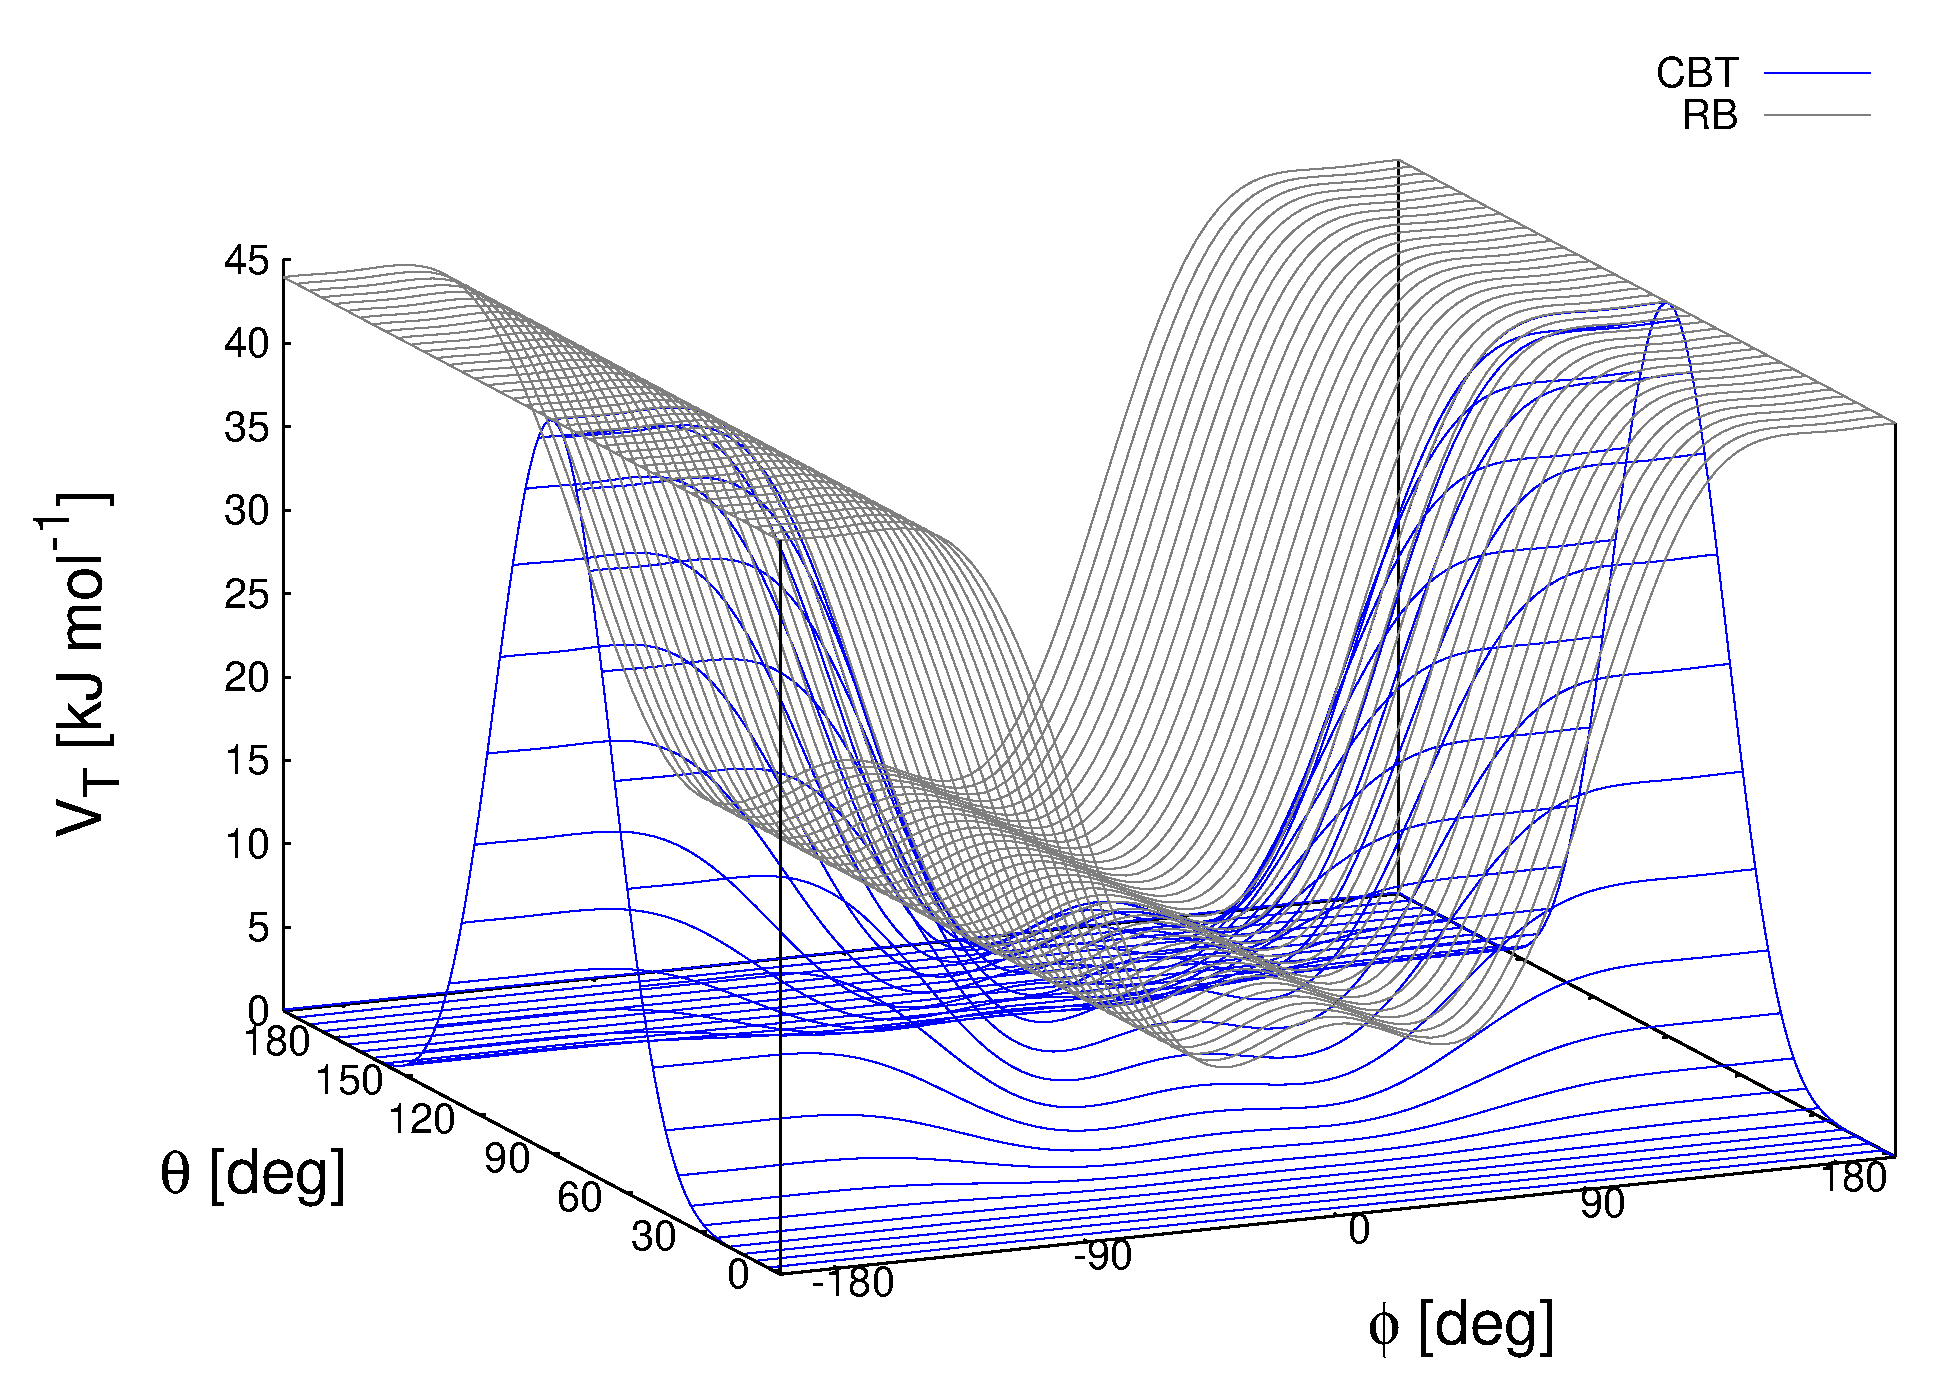
\includegraphics[width=10cm]{plots/fig-04}}
\caption{Blue: surface plot of the combined bending-torsion potential
(\ref{eq:CBT} with $k = 10$ kJ mol$^{-1}$, $a_0=2.41$, $a_1=-2.95$, $a_2=0.36$, $a_3=1.33$)
when, for simplicity, the bending angles behave the same ($\theta_1=\theta_2=\theta$).
Gray: the same torsion potential without the $\sin^{3}\theta$ terms (Ryckaert-Bellemans type).
$\phi$ is the dihedral angle.}
\label{fig:CBT}
\end{figure}
%
Additionally, the derivative of $V_{CBT}$ with respect to the Cartesian variables is straightforward:
%
\begin{equation}
\frac{\partial V_{\rm CBT}(\theta_{i-1},\theta_i,\phi_i)} {\partial \vec r_{l}} = \frac{\partial V_{\rm CBT}}{\partial \theta_{i-1}} \frac{\partial \theta_{i-1}}{\partial \vec r_{l}} +
                                                                                  \frac{\partial V_{\rm CBT}}{\partial \theta_{i  }} \frac{\partial \theta_{i  }}{\partial \vec r_{l}} +
                                                                                  \frac{\partial V_{\rm CBT}}{\partial \phi_{i    }} \frac{\partial \phi_{i    }}{\partial \vec r_{l}}
\label{eq:force_cbt}
\end{equation}
%
The CBT is based on a cosine form without multiplicity, so it can only be symmetrical around $0^{\circ}$.
To obtain an asymmetrical dihedral angle distribution (e.g. only one maximum in [$-180^{\circ}$:$180^{\circ}$] interval),
a standard torsion potential such as harmonic angle  or  periodic cosine potentials should be used instead of a CBT potential.
However, these two forms have the inconveniences of the force derivation ($1/\sin\phi$) and of the alignment of beads
($\theta_i$ or $\theta_{i-1} = 0^{\circ}, 180^{\circ}$).
Coupling such non-$\cos\phi$ potentials with $\sin^3\theta$ factors does not improve simulation stability since there are
cases in which $\theta$ and $\phi$ are simultaneously $180^{\circ}$. The integration at this step would be possible
(due to the cancelling of the torsion potential) but the next step would be singular
($\theta$ is not $180^{\circ}$ and $\phi$ is very close to $180^{\circ}$).

%\ifthenelse{\equal{\gmxlite}{1}}{}{
\subsection{Tabulated bonded interaction functions\index{tabulated bonded interaction function}}
\label{subsec:tabulatedinteraction}
For full flexibility, any functional shape can be used for
bonds, angles and dihedrals through user-supplied tabulated functions.
The functional shapes are:
\bea
V_b(r_{ij})      &=& k \, f^b_n(r_{ij}) \\
V_a(\tijk)       &=& k \, f^a_n(\tijk) \\
V_d(\phi_{ijkl}) &=& k \, f^d_n(\phi_{ijkl})
\eea
where $k$ is a force constant in units of energy
and $f$ is a cubic spline function; for details see \ssecref{cubicspline}.
For each interaction, the force constant $k$ and the table number $n$
are specified in the topology.
There are two different types of bonds, one that generates exclusions (type 8)
and one that does not (type 9).
For details see \tabref{topfile2}.
The table files are supplied to the {\tt mdrun} program.
After the table file name an underscore, the letter ``b'' for bonds,
``a'' for angles or ``d'' for dihedrals and the table number must be appended.
For example, a tabulated bond with $n=0$ can be read from the file {\tt table_b0.xvg}.
Multiple tables can be
supplied simply by adding files with different values of $n$, and are applied to the appropriate
bonds, as specified in the topology (\tabref{topfile2}).
The format for the table files is three fixed-format columns of any suitable width. These columns must contain $x$, $f(x)$, $-f'(x)$,
and the values of $x$ should be uniformly spaced. Requirements for entries in the topology
are given in~\tabref{topfile2}. 
The setup of the tables is as follows:
\\{\bf bonds}:
$x$ is the distance in nm. For distances beyond the table length,
{\tt mdrun} will quit with an error message.
\\{\bf angles}:
$x$ is the angle in degrees. The table should go from
0 up to and including 180 degrees; the derivative is taken in degrees.
\\{\bf dihedrals}:
$x$ is the dihedral angle in degrees. The table should go from
-180 up to and including 180 degrees;
the IUPAC/IUB convention is used, {\ie} zero is cis,
the derivative is taken in degrees.
%} % Brace matches ifthenelse test for gmxlite

\section{Restraints}
Special potentials are used for imposing restraints on the motion of
the system, either to avoid disastrous deviations, or to include
knowledge from experimental data. In either case they are not really
part of the force field and the reliability of the parameters is not
important. The potential forms, as implemented in {\gromacs}, are
mentioned just for the sake of completeness. Restraints and constraints
refer to quite different algorithms in {\gromacs}.

\subsection{Position restraints\swapindexquiet{position}{restraint}}
\label{subsec:positionrestraint}
These are used to restrain particles to fixed reference positions
$\ve{R}_i$. They can be used during equilibration in order to avoid
drastic rearrangements of critical parts ({\eg} to restrain motion
in a protein that is subjected to large solvent forces when the
solvent is not yet equilibrated). Another application is the
restraining of particles in a shell around a region that is simulated
in detail, while the shell is only approximated because it lacks
proper interaction from missing particles outside the
shell. Restraining will then maintain the integrity of the inner
part. For spherical shells, it is a wise procedure to make the force
constant depend on the radius, increasing from zero at the inner
boundary to a large value at the outer boundary. This feature has
not, however, been implemented in {\gromacs}.
\newcommand{\unitv}[1]{\hat{\bf #1}}
\newcommand{\halfje}[1]{\frac{#1}{2}}

The following form is used: 
\beq
V_{pr}(\ve{r}_i) = \halfje{1}k_{pr}|\rvi-\ve{R}_i|^2
\eeq
The potential is plotted in \figref{positionrestraint}.

\begin{figure}
\centerline{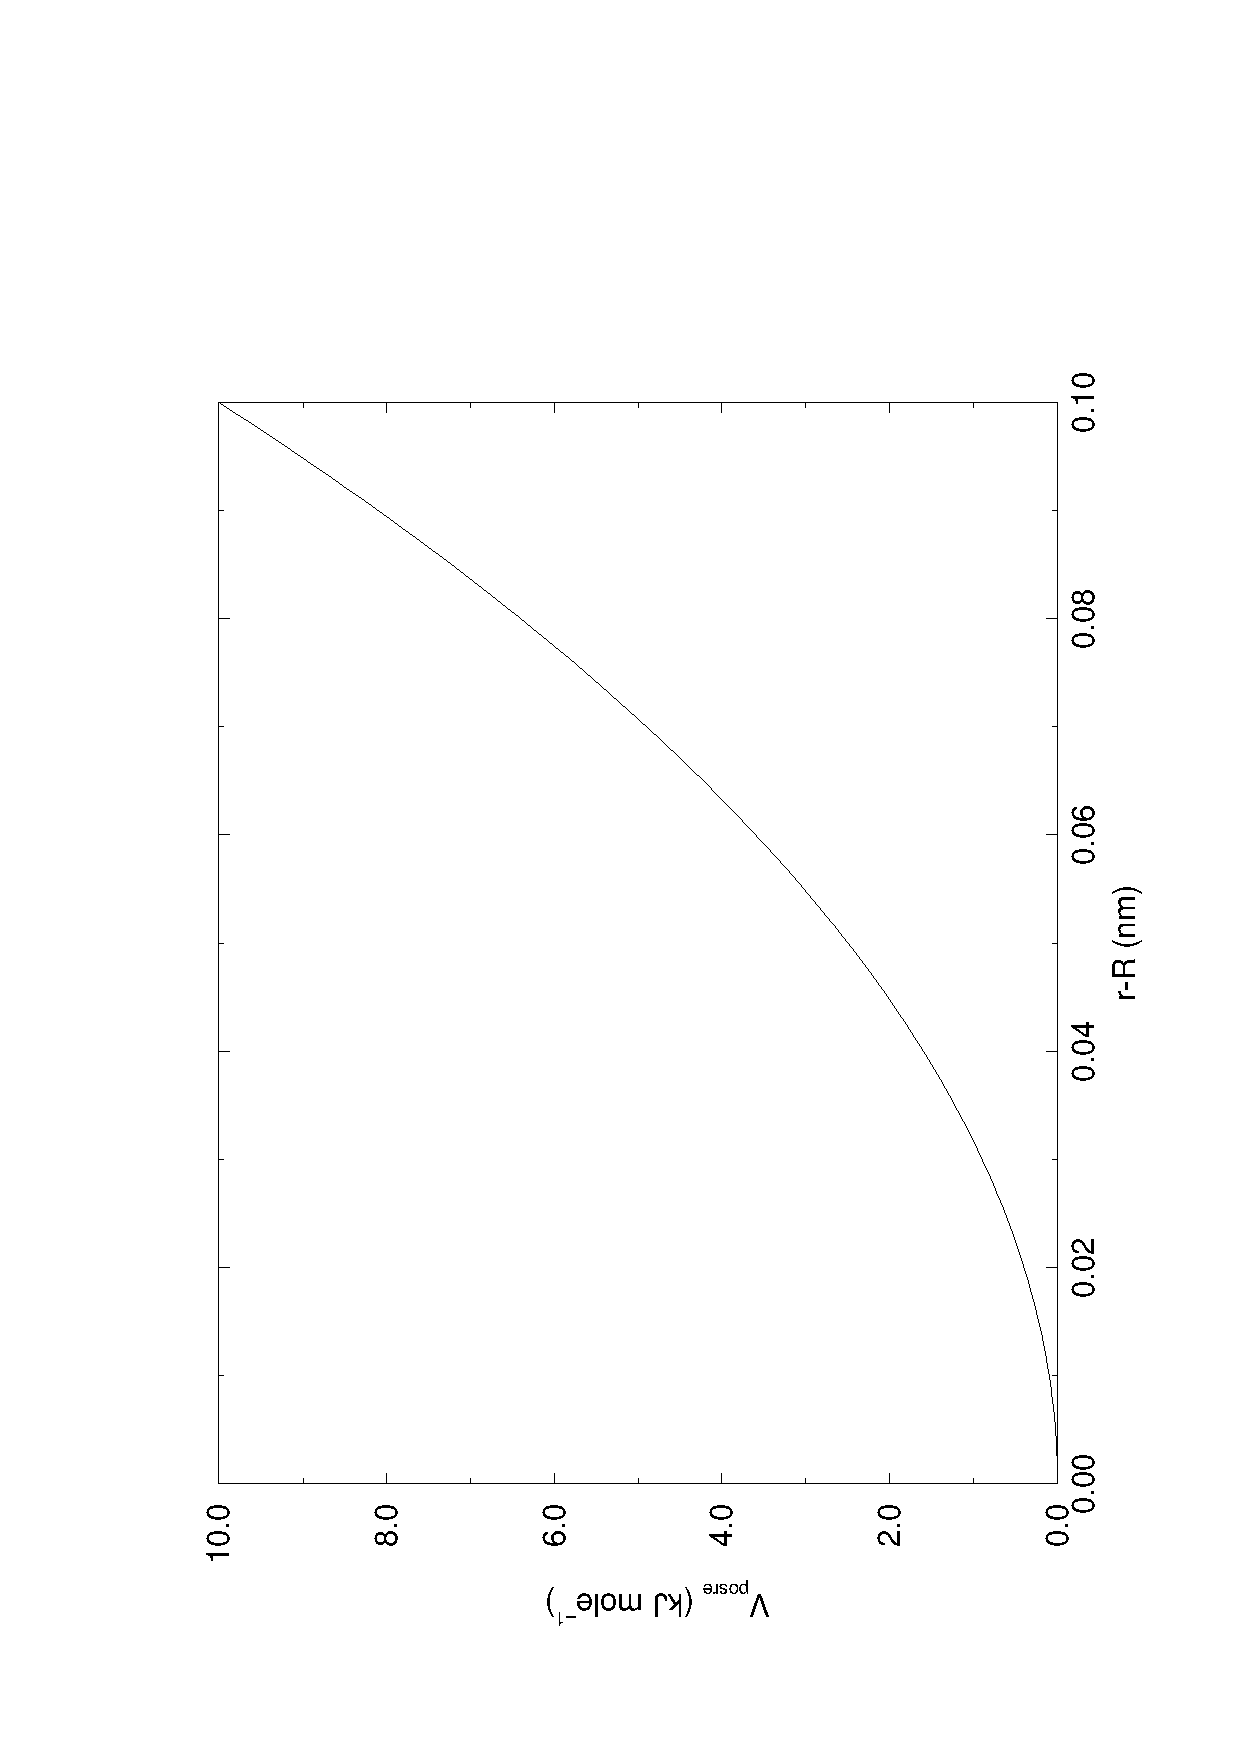
\includegraphics[width=8cm]{plots/f-pr}}
\caption{Position restraint potential.}
\label{fig:positionrestraint}
\end{figure}

The potential form can be rewritten without loss of generality as:
\beq
V_{pr}(\ve{r}_i) = \halfje{1} \left[ k_{pr}^x (x_i-X_i)^2 ~\unitv{x} + k_{pr}^y (y_i-Y_i)^2 ~\unitv{y} + k_{pr}^z (z_i-Z_i)^2 ~\unitv{z}\right]
\eeq

Now the forces are:
\beq
\begin{array}{rcl}
F_i^x &=& -k_{pr}^x~(x_i - X_i) \\
F_i^y &=& -k_{pr}^y~(y_i - Y_i) \\
F_i^z &=& -k_{pr}^z~(z_i - Z_i)
\end{array}
\eeq
Using three different force constants the position 
restraints can be turned on or off
in each spatial dimension; this means that atoms can be harmonically
restrained to a plane or a line.
Position restraints are applied to a special fixed list of atoms. Such a
list is usually generated by the {\tt \normindex{pdb2gmx}} program.

\subsection{\swapindex{Flat-bottomed}{position restraint}s}
\label{subsec:fbpositionrestraint}
Flat-bottomed position restraints can be used to restrain particles to 
part of the simulation volume. No force acts on the restrained
particle within the flat-bottomed region of the potential, however a
harmonic force acts to move the particle to the flat-bottomed region
if it is outside it. It is possible to apply normal and
flat-bottomed position restraints on the same particle (however, only
with the same reference position $\ve{R}_i$). The following general potential
is used (Figure~\ref{fig:fbposres}A):
\beq
 V_\mathrm{fb}(\ve{r}_i) = \frac{1}{2}k_\mathrm{fb} [d_g(\ve{r}_i;\ve{R}_i) - r_\mathrm{fb}]^2\,H[d_g(\ve{r}_i;\ve{R}_i) - r_\mathrm{fb}],
\eeq
where $\ve{R}_i$ is the reference position, $r_\mathrm{fb}$ is the distance
from the center with a flat potential, $k_\mathrm{fb}$ the force constant, and $H$ is the Heaviside step
function. The distance $d_g(\ve{r}_i;\ve{R}_i)$ from the reference
position depends on the geometry $g$ of the flat-bottomed potential.

\begin{figure}
\centerline{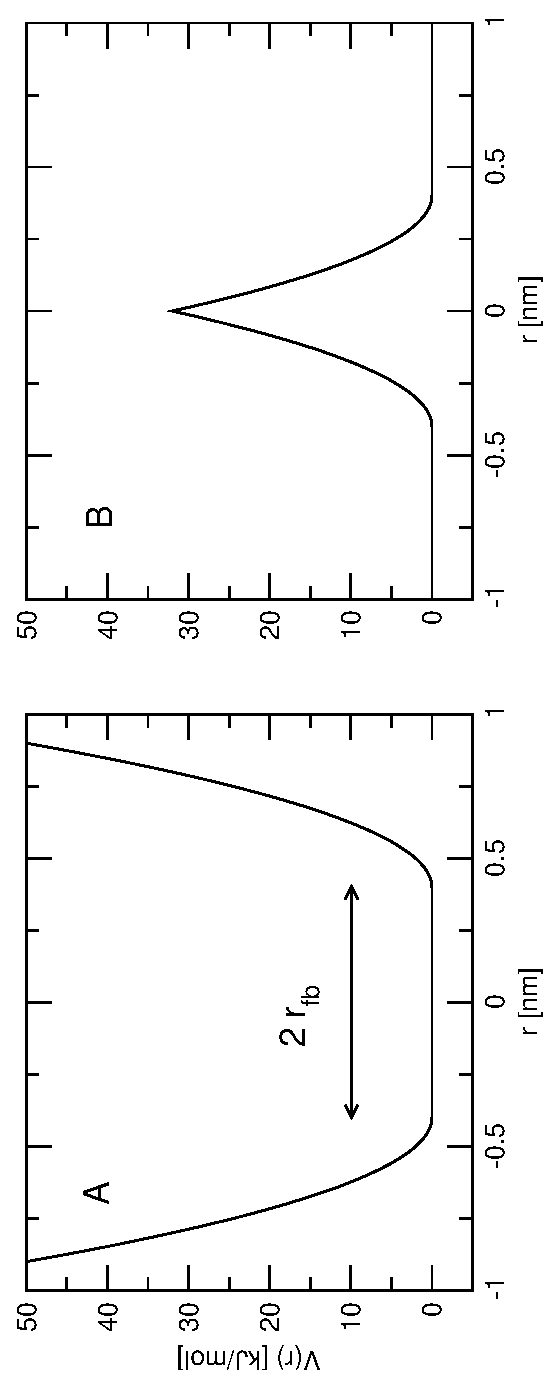
\includegraphics[width=10cm]{plots/fbposres}}
\caption{Flat-bottomed position restraint potential. (A) Not
  inverted, (B) inverted.}
\label{fig:fbposres}
\end{figure}

The following geometries for the flat-bottomed potential are supported:\newline
{\bfseries Sphere} ($g =1$): The particle is kept in a sphere of given
radius. The force acts towards the center of the sphere. The following distance calculation is used:
\beq
  d_g(\ve{r}_i;\ve{R}_i) = |\ve{r}_i-\ve{R}_i|
\eeq
{\bfseries Cylinder} ($g=6,7,8$): The particle is kept in a cylinder of given radius
parallel to the $x$ ($g=6$), $y$ ($g=7$), or $z$-axis ($g=8$). For backwards compatibility, setting
$g=2$ is mapped to $g=8$ in the code so that old {\tt .tpr} files and topologies work.  
The force from the flat-bottomed potential acts towards the axis of the cylinder. 
The component of the force parallel to the cylinder axis is zero.
For a cylinder aligned along the $z$-axis:
\beq
 d_g(\ve{r}_i;\ve{R}_i) = \sqrt{ (x_i-X_i)^2 + (y_i - Y_i)^2 }
\eeq
{\bfseries Layer} ($g=3,4,5$): The particle is kept in a layer defined by the
thickness and the normal of the layer. The layer normal can be parallel to the $x$, $y$, or
$z$-axis. The force acts parallel to the layer normal.\\
\beq
 d_g(\ve{r}_i;\ve{R}_i) = |x_i-X_i|, \;\;\;\mbox{or}\;\;\; 
 d_g(\ve{r}_i;\ve{R}_i) = |y_i-Y_i|, \;\;\;\mbox{or}\;\;\; 
d_g(\ve{r}_i;\ve{R}_i) = |z_i-Z_i|.
\eeq

It is possible to apply multiple independent flat-bottomed position
restraints of different geometry on one particle. For example, applying
a cylinder and a layer in $z$ keeps a particle within a
disk. Applying three layers in $x$, $y$, and $z$ keeps the particle within a cuboid.

In addition, it is possible to invert the restrained region with the
unrestrained region, leading to a potential that acts to keep the particle {\it outside} of the volume
defined by $\ve{R}_i$, $g$, and $r_\mathrm{fb}$. That feature is
switched on by defining a negative $r_\mathrm{fb}$ in the
topology. The following potential is used (Figure~\ref{fig:fbposres}B):
\beq
  V_\mathrm{fb}^{\mathrm{inv}}(\ve{r}_i) = \frac{1}{2}k_\mathrm{fb}
  [d_g(\ve{r}_i;\ve{R}_i) - |r_\mathrm{fb}|]^2\,
  H[ -(d_g(\ve{r}_i;\ve{R}_i) - |r_\mathrm{fb}|)].
\eeq



%\ifthenelse{\equal{\gmxlite}{1}}{}{
\subsection{Angle restraints\swapindexquiet{angle}{restraint}}
\label{subsec:anglerestraint}
These are used to restrain the angle between two pairs of particles
or between one pair of particles and the $z$-axis.
The functional form is similar to that of a proper dihedral.
For two pairs of atoms: 
\beq
V_{ar}(\ve{r}_i,\ve{r}_j,\ve{r}_k,\ve{r}_l)
        = k_{ar}(1 - \cos(n (\theta - \theta_0))
        )
,~~~~\mbox{where}~~
\theta = \arccos\left(\frac{\ve{r}_j -\ve{r}_i}{\|\ve{r}_j -\ve{r}_i\|}
 \cdot \frac{\ve{r}_l -\ve{r}_k}{\|\ve{r}_l -\ve{r}_k\|} \right)
\eeq
For one pair of atoms and the $z$-axis: 
\beq
V_{ar}(\ve{r}_i,\ve{r}_j) = k_{ar}(1 - \cos(n (\theta - \theta_0))
        )
,~~~~\mbox{where}~~
\theta = \arccos\left(\frac{\ve{r}_j -\ve{r}_i}{\|\ve{r}_j -\ve{r}_i\|}
 \cdot \left( \begin{array}{c} 0 \\ 0 \\ 1 \\ \end{array} \right) \right)
\eeq
A multiplicity ($n$) of 2 is useful when you do not want to distinguish
between parallel and anti-parallel vectors.
The equilibrium angle $\theta$ should be between 0 and 180 degrees
for multiplicity 1 and between 0 and 90 degrees for multiplicity 2.


\subsection{Dihedral restraints\swapindexquiet{dihedral}{restraint}}
\label{subsec:dihedralrestraint}
These are used to restrain the dihedral angle $\phi$ defined by four particles
as in an improper dihedral (sec.~\ref{sec:imp}) but with a slightly
modified potential. Using:
\beq
\phi' = \left(\phi-\phi_0\right) ~{\rm MOD}~ 2\pi
\label{eqn:dphi}
\eeq
where $\phi_0$ is the reference angle, the potential is defined as:
\beq
V_{dihr}(\phi') ~=~ \left\{
\begin{array}{lcllll}
\half k_{dihr}(\phi'-\phi_0-\Delta\phi)^2      
                &\mbox{for}&     \phi' & >   & \Delta\phi       \\[1.5ex]
0               &\mbox{for}&     \phi' & \le & \Delta\phi       \\[1.5ex]
\end{array}\right.
\label{eqn:dihre}
\eeq
where $\Delta\phi$ is a user defined angle and $k_{dihr}$ is the force 
constant.
{\bf Note} that in the input in topology files, angles are given in degrees and
force constants in kJ/mol/rad$^2$.
%} % Brace matches ifthenelse test for gmxlite

\subsection{Distance restraints\swapindexquiet{distance}{restraint}}
\label{subsec:distancerestraint}
Distance restraints 
add a penalty to the potential when the distance between specified
pairs of atoms exceeds a threshold value. They are normally used to
impose experimental restraints from, for instance, experiments in nuclear
magnetic resonance (NMR), on the motion of the system. Thus, MD can be
used for structure refinement using NMR data\index{nmr
refinement}\index{refinement,nmr}.
In {\gromacs} there are three ways to impose restraints on pairs of atoms:
\begin{itemize}
\item Simple harmonic restraints: use {\tt [ bonds ]} type 6
%\ifthenelse{\equal{\gmxlite}{1}}
{.}
{(see \secref{excl}).}
\item\label{subsec:harmonicrestraint}Piecewise linear/harmonic restraints: {\tt [ bonds ]} type 10.
\item Complex NMR distance restraints, optionally with pair, time and/or
ensemble averaging.
\end{itemize}
The last two options will be detailed now.

The potential form for distance restraints is quadratic below a specified
lower bound and between two specified upper bounds, and linear beyond the
largest bound (see \figref{dist}).
\beq
V_{dr}(r_{ij}) ~=~ \left\{
\begin{array}{lcllllll}
\half k_{dr}(r_{ij}-r_0)^2      
                &\mbox{for}&     &     & r_{ij} & < & r_0       \\[1.5ex]
0               &\mbox{for}& r_0 & \le & r_{ij} & < & r_1       \\[1.5ex]
\half k_{dr}(r_{ij}-r_1)^2      
                &\mbox{for}& r_1 & \le & r_{ij} & < & r_2       \\[1.5ex]
\half k_{dr}(r_2-r_1)(2r_{ij}-r_2-r_1)  
                &\mbox{for}& r_2 & \le & r_{ij} &   &
\end{array}\right.
\label{eqn:disre}
\eeq

\begin{figure}
\centerline{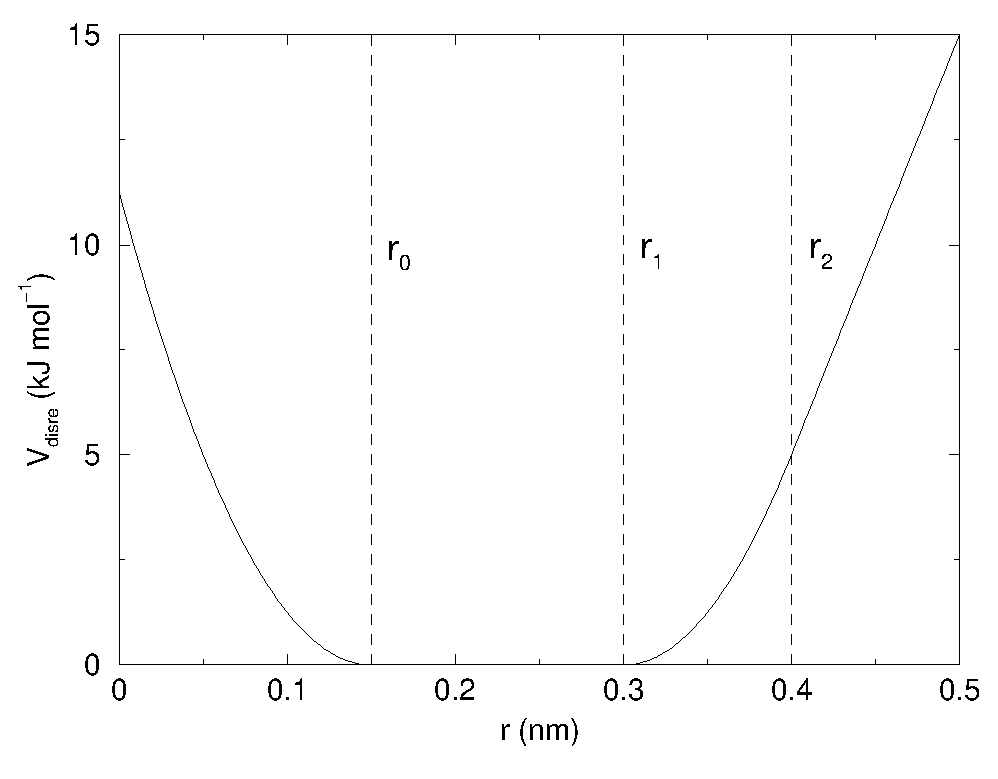
\includegraphics[width=8cm]{plots/f-dr}}
\caption{Distance Restraint potential.}
\label{fig:dist}
\end{figure}

The forces are
\beq
\ve{F}_i~=~ \left\{
\begin{array}{lcllllll}
-k_{dr}(r_{ij}-r_0)\frac{\rvij}{r_{ij}} 
                &\mbox{for}&     &     & r_{ij} & < & r_0       \\[1.5ex]
0               &\mbox{for}& r_0 & \le & r_{ij} & < & r_1       \\[1.5ex]
-k_{dr}(r_{ij}-r_1)\frac{\rvij}{r_{ij}} 
                &\mbox{for}& r_1 & \le & r_{ij} & < & r_2       \\[1.5ex]
-k_{dr}(r_2-r_1)\frac{\rvij}{r_{ij}}    
                &\mbox{for}& r_2 & \le & r_{ij} &   &
\end{array} \right.
\eeq

For restraints not derived from NMR data, this functionality
will usually suffice and a section of {\tt [ bonds ]} type 10
can be used to apply individual restraints between pairs of
%\ifthenelse{\equal{\gmxlite}{1}}{atoms.}{
atoms, see \ssecref{topfile}.
%} % Brace matches ifthenelse test for gmxlite 
For applying restraints derived from NMR measurements, more complex
functionality might be required, which is provided through
the {\tt [~distance_restraints~]} section and is described below.

%\ifthenelse{\equal{\gmxlite}{1}}{}{
\subsubsection{Time averaging\swapindexquiet{time-averaged}{distance restraint}}
Distance restraints based on instantaneous distances can potentially reduce
the fluctuations in a molecule significantly. This problem can be overcome by restraining
to a {\em time averaged} distance~\cite{Torda89}.
The forces with time averaging are:
\beq
\ve{F}_i~=~ \left\{
\begin{array}{lcllllll}
-k^a_{dr}(\bar{r}_{ij}-r_0)\frac{\rvij}{r_{ij}}   
                &\mbox{for}&     &     & \bar{r}_{ij} & < & r_0 \\[1.5ex]
0               &\mbox{for}& r_0 & \le & \bar{r}_{ij} & < & r_1 \\[1.5ex]
-k^a_{dr}(\bar{r}_{ij}-r_1)\frac{\rvij}{r_{ij}}   
                &\mbox{for}& r_1 & \le & \bar{r}_{ij} & < & r_2 \\[1.5ex]
-k^a_{dr}(r_2-r_1)\frac{\rvij}{r_{ij}}    
                &\mbox{for}& r_2 & \le & \bar{r}_{ij} &   &
\end{array} \right.
\eeq
where $\bar{r}_{ij}$ is given by an exponential running average with decay time $\tau$:
\beq
\bar{r}_{ij} ~=~ < r_{ij}^{-3} >^{-1/3}
\label{eqn:rav}
\eeq
The force constant $k^a_{dr}$ is switched on slowly to compensate for
the lack of history at the beginning of the simulation:
\beq
k^a_{dr} = k_{dr} \left(1-\exp\left(-\frac{t}{\tau}\right)\right)
\eeq
Because of the time averaging, we can no longer speak of a distance restraint
potential.

This way an atom can satisfy two incompatible distance restraints 
{\em on average} by moving between two positions. 
An example would be an amino acid side-chain that is rotating around
its $\chi$ dihedral angle, thereby coming close to various other groups.
Such a mobile side chain can give rise to multiple NOEs that can not be
fulfilled by a single structure.

The computation of the time
averaged distance in the {\tt mdrun} program is done in the following fashion:
\beq
\begin{array}{rcl}
\overline{r^{-3}}_{ij}(0)       &=& r_{ij}(0)^{-3}      \\
\overline{r^{-3}}_{ij}(t)       &=& \overline{r^{-3}}_{ij}(t-\Delta t)~\exp{\left(-\frac{\Delta t}{\tau}\right)} + r_{ij}(t)^{-3}\left[1-\exp{\left(-\frac{\Delta t}{\tau}\right)}\right]
\label{eqn:ravdisre}
\end{array}
\eeq

When a pair is within the bounds, it can still feel a force
because the time averaged distance can still be beyond a bound.
To prevent the protons from being pulled too close together, a mixed
approach can be used. In this approach, the penalty is zero when the
instantaneous distance is within the bounds, otherwise the violation is
the square root of the product of the instantaneous violation and the 
time averaged violation:
\beq
\ve{F}_i~=~ \left\{
\begin{array}{lclll}
k^a_{dr}\sqrt{(r_{ij}-r_0)(\bar{r}_{ij}-r_0)}\frac{\rvij}{r_{ij}}   
    & \mbox{for} & r_{ij} < r_0 & \mbox{and} & \bar{r}_{ij} < r_0 \\[1.5ex]
-k^a _{dr} \,
  \mbox{min}\left(\sqrt{(r_{ij}-r_1)(\bar{r}_{ij}-r_1)},r_2-r_1\right)
  \frac{\rvij}{r_{ij}}   
    & \mbox{for} & r_{ij} > r_1 & \mbox{and} & \bar{r}_{ij} > r_1 \\[1.5ex]
0               &\mbox{otherwise}
\end{array} \right.
\eeq

\subsubsection{Averaging over multiple pairs\swapindexquiet{ensemble-averaged}{distance restraint}} 

Sometimes it is unclear from experimental data which atom pair
gives rise to a single NOE, in other occasions it can be obvious that
more than one pair contributes due to the symmetry of the system, {\eg} a
methyl group with three protons. For such a group, it is not possible 
to distinguish between the protons, therefore they should all be taken into
account when calculating the distance between this methyl group and another
proton (or group of protons).
Due to the physical nature of magnetic resonance, the intensity of the
NOE signal is inversely proportional to the sixth power of the inter-atomic 
distance.
Thus, when combining atom pairs, 
a fixed list of $N$ restraints may be taken together, 
where the apparent ``distance'' is given by:
\beq
r_N(t) = \left [\sum_{n=1}^{N} \bar{r}_{n}(t)^{-6} \right]^{-1/6}
\label{eqn:rsix}
\eeq
where we use $r_{ij}$ or \eqnref{rav} for the $\bar{r}_{n}$.
The $r_N$ of the instantaneous and time-averaged distances
can be combined to do a mixed restraining, as indicated above.
As more pairs of protons contribute to the same NOE signal, the intensity
will increase, and the summed ``distance'' will be shorter than any of
its components due to the reciprocal summation. 

There are two options for distributing the forces over the atom pairs.
In the conservative option, the force is defined as the derivative of the
restraint potential with respect to the coordinates. This results in
a conservative potential when time averaging is not used.
The force distribution over the pairs is proportional to $r^{-6}$.
This means that a close pair feels a much larger force than a distant pair,
which might lead to a molecule that is ``too rigid.''
The other option is an equal force distribution. In this case each pair
feels $1/N$ of the derivative of the restraint potential with respect to 
$r_N$. The advantage of this method is that more conformations might be
sampled, but the non-conservative nature of the forces can lead to
local heating of the protons.

It is also possible to use {\em ensemble averaging} using multiple
(protein)  molecules. In this case the bounds should be lowered as in:
\beq
\begin{array}{rcl}
r_1     &~=~&   r_1 * M^{-1/6}  \\
r_2     &~=~&   r_2 * M^{-1/6}
\end{array}
\eeq
where $M$ is the number of molecules. The {\gromacs} preprocessor {\tt grompp}
can do this automatically when the appropriate option is given.
The resulting ``distance'' is 
then used to calculate the scalar force according to:
\beq
\ve{F}_i~=~\left\{
\begin{array}{rcl}
~& 0 \hspace{4cm}  & r_{N} < r_1         \\
 & k_{dr}(r_{N}-r_1)\frac{\rvij}{r_{ij}} & r_1 \le r_{N} < r_2 \\
 & k_{dr}(r_2-r_1)\frac{\rvij}{r_{ij}}    & r_{N} \ge r_2 
\end{array} \right.
\eeq
where $i$ and $j$ denote the atoms of all the 
pairs that contribute to the NOE signal.

\subsubsection{Using distance restraints}

A list of distance restrains based on NOE data can be added to a molecule
definition in your topology file, like in the following example:

\begin{verbatim}
[ distance_restraints ]
; ai   aj   type   index   type'      low     up1     up2     fac
10     16      1       0       1      0.0     0.3     0.4     1.0
10     28      1       1       1      0.0     0.3     0.4     1.0
10     46      1       1       1      0.0     0.3     0.4     1.0
16     22      1       2       1      0.0     0.3     0.4     2.5
16     34      1       3       1      0.0     0.5     0.6     1.0
\end{verbatim}

In this example a number of features can be found.  In columns {\tt
ai} and {\tt aj} you find the atom numbers of the particles to be
restrained. The {\tt type} column should always be 1.  As explained in
~\ssecref{distancerestraint}, multiple distances can contribute to a single NOE
signal. In the topology this can be set using the {\tt index}
column. In our example, the restraints 10-28 and 10-46 both have index
1, therefore they are treated simultaneously.  An extra requirement
for treating restraints together is that the restraints must be on
successive lines, without any other intervening restraint.  The {\tt
type'} column will usually be 1, but can be set to 2 to obtain a
distance restraint that will never be time- and ensemble-averaged;
this can be useful for restraining hydrogen bonds.  The columns {\tt
low}, {\tt up1}, and {\tt up2} hold the values of $r_0$, $r_1$, and
$r_2$ from ~\eqnref{disre}.  In some cases it can be useful to have
different force constants for some restraints; this is controlled by
the column {\tt fac}.  The force constant in the parameter file is
multiplied by the value in the column {\tt fac} for each restraint.
%} % Brace matches ifthenelse test for gmxlite

\newcommand{\SSS}{{\mathbf S}}
\newcommand{\DD}{{\mathbf D}}
\newcommand{\RR}{{\mathbf R}}

%\ifthenelse{\equal{\gmxlite}{1}}{}{
\subsection{Orientation restraints\swapindexquiet{orientation}{restraint}}
\label{subsec:orientationrestraint}
This section describes how orientations between vectors,
as measured in certain NMR experiments, can be calculated
and restrained in MD simulations.
The presented refinement methodology and a comparison of results
with and without time and ensemble averaging have been
published~\cite{Hess2003}.
\subsubsection{Theory}
In an NMR experiment, orientations of vectors can be measured when a 
molecule does not tumble completely isotropically in the solvent.
Two examples of such orientation measurements are
residual \normindex{dipolar couplings}
(between two nuclei) or chemical shift anisotropies.
An observable for a vector $\ve{r}_i$ can be written as follows:
\beq
\delta_i = \frac{2}{3} \mbox{tr}(\SSS\DD_i)
\eeq
where $\SSS$ is the dimensionless order tensor of the molecule.
The tensor $\DD_i$ is given by:
\beq
\label{orient_def}
\DD_i = \frac{c_i}{\|\ve{r}_i\|^\alpha} \left(
%\begin{array}{lll}
%3 r_x r_x - \ve{r}\cdot\ve{r} & 3 r_x r_y & 3 r_x r_z \\
%3 r_x r_y                     & 3 r_y r_y - \ve{r}\cdot\ve{r} & 3yz \\
%3 r_x r_z                     & 3 r_y r_z & 3 r_z r_z - \ve{r}\cdot\ve{r}
%\end{array} \right)
\begin{array}{lll}
3 x x - 1 & 3 x y     & 3 x z     \\
3 x y     & 3 y y - 1 & 3 y z     \\
3 x z     & 3 y z     & 3 z z - 1 \\
\end{array} \right)
\eeq
\beq
\mbox{with:} \quad 
x=\frac{r_{i,x}}{\|\ve{r}_i\|}, \quad
y=\frac{r_{i,y}}{\|\ve{r}_i\|}, \quad 
z=\frac{r_{i,z}}{\|\ve{r}_i\|}
\eeq
For a dipolar coupling $\ve{r}_i$ is the vector connecting the two
nuclei, $\alpha=3$ and the constant $c_i$ is given by:
\beq
c_i = \frac{\mu_0}{4\pi} \gamma_1^i \gamma_2^i \frac{\hbar}{4\pi}
\eeq
where $\gamma_1^i$ and $\gamma_2^i$ are the gyromagnetic ratios of the
two nuclei.

The order tensor is symmetric and has trace zero. Using a rotation matrix
${\mathbf T}$ it can be transformed into the following form:
\beq
{\mathbf T}^T \SSS {\mathbf T} = s \left( \begin{array}{ccc}
-\frac{1}{2}(1-\eta) & 0                    & 0 \\
0                    & -\frac{1}{2}(1+\eta) & 0 \\
0                    & 0                    & 1
\end{array} \right)
\eeq
where $-1 \leq s \leq 1$ and $0 \leq \eta \leq 1$.
$s$ is called the order parameter and $\eta$ the asymmetry of the
order tensor $\SSS$. When the molecule tumbles isotropically in the
solvent, $s$ is zero, and no orientational effects can be observed
because all $\delta_i$ are zero.

%\newpage

\subsubsection{Calculating orientations in a simulation}
For reasons which are explained below, the $\DD$ matrices are calculated
which respect to a reference orientation of the molecule. The orientation
is defined by a rotation matrix $\RR$, which is needed to least-squares fit
the current coordinates of a selected set of atoms onto
a reference conformation. The reference conformation is the starting
conformation of the simulation. In case of ensemble averaging, which will
be treated later, the structure is taken from the first subsystem.
The calculated $\DD_i^c$ matrix is given by:
\begin{equation}
\label{D_rot}
\DD_i^c(t) = \RR(t) \DD_i(t) \RR^T(t)
\end{equation}
The calculated orientation for vector $i$ is given by:
\beq
\delta^c_i(t) = \frac{2}{3} \mbox{tr}(\SSS(t)\DD_i^c(t))
\eeq
The order tensor $\SSS(t)$ is usually unknown.
A reasonable choice for the order tensor is the tensor
which minimizes the (weighted) mean square difference between the calculated
and the observed orientations:
\begin{equation}
\label{S_msd}
MSD(t) = \left(\sum_{i=1}^N w_i\right)^{-1} \sum_{i=1}^N w_i (\delta_i^c (t) -\delta_i^{exp})^2
\end{equation}
To properly combine different types of measurements, the unit of $w_i$ should
be such that all terms are dimensionless. This means the unit of $w_i$
is the unit of $\delta_i$ to the power $-2$.
{\bf Note} that scaling all $w_i$ with a constant factor does not influence
the order tensor.

\subsubsection{Time averaging}
Since the tensors $\DD_i$ fluctuate rapidly in time, much faster than can
be observed in an experiment, they should be averaged over time in the simulation.
However, in a simulation the time and the number of copies of
a molecule are limited. Usually one can not obtain a converged average
of the $\DD_i$ tensors over all orientations of the molecule.
If one assumes that the average orientations of the $\ve{r}_i$ vectors
within the molecule converge much faster than the tumbling time of
the molecule, the tensor can be averaged in an axis system that 
rotates with the molecule, as expressed by equation~(\ref{D_rot}).
The time-averaged tensors are calculated
using an exponentially decaying memory function:
\beq
\DD^a_i(t) = \frac{\displaystyle
\int_{u=t_0}^t \DD^c_i(u) \exp\left(-\frac{t-u}{\tau}\right)\mbox{d} u
}{\displaystyle
\int_{u=t_0}^t \exp\left(-\frac{t-u}{\tau}\right)\mbox{d} u
}
\eeq
Assuming that the order tensor $\SSS$ fluctuates slower than the
$\DD_i$, the time-averaged orientation can be calculated as:
\beq
\delta_i^a(t) = \frac{2}{3} \mbox{tr}(\SSS(t) \DD_i^a(t))
\eeq
where the order tensor $\SSS(t)$ is calculated using expression~(\ref{S_msd})
with $\delta_i^c(t)$ replaced by $\delta_i^a(t)$.

\subsubsection{Restraining}
The simulated structure can be restrained by applying a force proportional
to the difference between the calculated and the experimental orientations.
When no time averaging is applied, a proper potential can be defined as:
\beq
V = \frac{1}{2} k \sum_{i=1}^N w_i (\delta_i^c (t) -\delta_i^{exp})^2
\eeq
where the unit of $k$ is the unit of energy.
Thus the effective force constant for restraint $i$ is $k w_i$.
The forces are given by minus the gradient of $V$.
The force $\ve{F}\!_i$ working on vector $\ve{r}_i$ is:
\begin{eqnarray*}
\ve{F}\!_i(t) 
& = & - \frac{\mbox{d} V}{\mbox{d}\ve{r}_i} \\
& = & -k w_i (\delta_i^c (t) -\delta_i^{exp}) \frac{\mbox{d} \delta_i (t)}{\mbox{d}\ve{r}_i} \\
& = & -k w_i (\delta_i^c (t) -\delta_i^{exp})
\frac{2 c_i}{\|\ve{r}\|^{2+\alpha}} \left(2 \RR^T \SSS \RR \ve{r}_i - \frac{2+\alpha}{\|\ve{r}\|^2} \mbox{tr}(\RR^T \SSS \RR \ve{r}_i \ve{r}_i^T) \ve{r}_i \right)
\end{eqnarray*}

\subsubsection{Ensemble averaging}
Ensemble averaging can be applied by simulating a system of $M$ subsystems
that each contain an identical set of orientation restraints. The systems only
interact via the orientation restraint potential which is defined as:
\beq
V = M \frac{1}{2} k \sum_{i=1}^N w_i 
\langle \delta_i^c (t) -\delta_i^{exp} \rangle^2
\eeq
The force on vector $\ve{r}_{i,m}$ in subsystem $m$ is given by:
\beq
\ve{F}\!_{i,m}(t) = - \frac{\mbox{d} V}{\mbox{d}\ve{r}_{i,m}} =
-k w_i \langle \delta_i^c (t) -\delta_i^{exp} \rangle \frac{\mbox{d} \delta_{i,m}^c (t)}{\mbox{d}\ve{r}_{i,m}} \\
\eeq 

\subsubsection{Time averaging}
When using time averaging it is not possible to define a potential.
We can still define a quantity that gives a rough idea of the energy
stored in the restraints:
\beq
V = M \frac{1}{2} k^a \sum_{i=1}^N w_i 
\langle \delta_i^a (t) -\delta_i^{exp} \rangle^2
\eeq
The force constant $k_a$ is switched on slowly to compensate for the
lack of history at times close to $t_0$. It is exactly proportional
to the amount of average that has been accumulated:
\beq
k^a =
 k \, \frac{1}{\tau}\int_{u=t_0}^t \exp\left(-\frac{t-u}{\tau}\right)\mbox{d} u
\eeq
What really matters is the definition of the force. It is chosen to
be proportional to the square root of the product of the time-averaged
and the instantaneous deviation.
Using only the time-averaged deviation induces large oscillations.
The force is given by:
\beq
\ve{F}\!_{i,m}(t) =
%\left\{ \begin{array}{ll}
%0 & \mbox{for} \quad \langle \delta_i^a (t) -\delta_i^{exp} \rangle \langle \delta_i (t) -\delta_i^{exp} \rangle \leq 0 \\
%... & \mbox{for} \quad \langle \delta_i^a (t) -\delta_i^{exp} \rangle \langle \delta_i (t) -\delta_i^{exp} \rangle > 0 
%\end{array}
%\right.
\left\{ \begin{array}{ll}
0 & \quad \mbox{for} \quad a\, b \leq 0 \\
\displaystyle
k^a w_i \frac{a}{|a|} \sqrt{a\, b} \, \frac{\mbox{d} \delta_{i,m}^c (t)}{\mbox{d}\ve{r}_{i,m}}
& \quad \mbox{for} \quad a\, b > 0 
\end{array}
\right.
\eeq
\begin{eqnarray*}
a &=& \langle \delta_i^a (t) -\delta_i^{exp} \rangle \\
b &=& \langle \delta_i^c (t) -\delta_i^{exp} \rangle
\end{eqnarray*}

\subsubsection{Using orientation restraints}
Orientation restraints can be added to a molecule definition in
the topology file in the section {\tt [~orientation_restraints~]}.
Here we give an example section containing five N-H residual dipolar
coupling restraints:

\begin{verbatim}
[ orientation_restraints ]
; ai   aj  type  exp.  label  alpha    const.     obs.   weight
;                                Hz      nm^3       Hz    Hz^-2
  31   32     1     1      3      3     6.083    -6.73      1.0
  43   44     1     1      4      3     6.083    -7.87      1.0
  55   56     1     1      5      3     6.083    -7.13      1.0
  65   66     1     1      6      3     6.083    -2.57      1.0
  73   74     1     1      7      3     6.083    -2.10      1.0
\end{verbatim}

The unit of the observable is Hz, but one can choose any other unit.
In columns {\tt
ai} and {\tt aj} you find the atom numbers of the particles to be
restrained. The {\tt type} column should always be 1.
The {\tt exp.} column denotes the experiment number, starting
at 1. For each experiment a separate order tensor $\SSS$
is optimized. The label should be a unique number larger than zero
for each restraint. The {\tt alpha} column contains the power $\alpha$ 
that is used in equation~(\ref{orient_def}) to calculate the orientation.
The {\tt const.} column contains the constant $c_i$ used in the same
equation. The constant should have the unit of the observable times
nm$^\alpha$. The column {\tt obs.} contains the observable, in any
unit you like. The last column contains the weights $w_i$; the unit
should be the inverse of the square of the unit of the observable.

Some parameters for orientation restraints can be specified in the
{\tt grompp.mdp} file, for a study of the effect of different
force constants and averaging times and ensemble averaging see~\cite{Hess2003}.
%} % Brace matches ifthenelse test for gmxlite

%\ifthenelse{\equal{\gmxlite}{1}}{}{
\section{Polarization}
Polarization can be treated by {\gromacs} by attaching
\normindex{shell} (\normindex{Drude}) particles to atoms and/or
virtual sites. The energy of the shell particle is then minimized at
each time step in order to remain on the Born-Oppenheimer surface.

\subsection{Simple polarization}
This is merely a harmonic potential with equilibrium distance 0.

\subsection{Water polarization}
A special potential for water that allows anisotropic polarization of
a single shell particle~\cite{Maaren2001a}.

\subsection{Thole polarization}
Based on early work by \normindex{Thole}~\cite{Thole81}, Roux and
coworkers have implemented potentials for molecules like
ethanol~\cite{Lamoureux2003a,Lamoureux2003b,Noskov2005a}. Within such
molecules, there are intra-molecular interactions between shell
particles, however these must be screened because full Coulomb would
be too strong. The potential between two shell particles $i$ and $j$ is:
\newcommand{\rbij}{\bar{r}_{ij}}
\beq
V_{thole} ~=~ \frac{q_i q_j}{r_{ij}}\left[1-\left(1+\frac{\rbij}{2}\right){\rm exp}^{-\rbij}\right]
\eeq
{\bf Note} that there is a sign error in Equation~1 of Noskov {\em et al.}~\cite{Noskov2005a}:
\beq
\rbij ~=~ a\frac{r_{ij}}{(\alpha_i \alpha_j)^{1/6}}
\eeq
where $a$ is a magic (dimensionless) constant, usually chosen to be
2.6~\cite{Noskov2005a}; $\alpha_i$ and $\alpha_j$ are the polarizabilities
of the respective shell particles.

%} % Brace matches ifthenelse test for gmxlite

%\ifthenelse{\equal{\gmxlite}{1}}{}{
\section{Free energy interactions}
\label{sec:feia}
\index{free energy interactions}
\newcommand{\LAM}{\lambda}
\newcommand{\LL}{(1-\LAM)}
\newcommand{\dvdl}[1]{\frac{\partial #1}{\partial \LAM}}
This section describes the $\lambda$-dependence of the potentials
used for free energy calculations (see \secref{fecalc}).
All common types of potentials and constraints can be
interpolated smoothly from state A ($\lambda=0$) to state B
($\lambda=1$) and vice versa.
All bonded interactions are interpolated by linear interpolation
of the interaction parameters. Non-bonded interactions can be
interpolated linearly or via soft-core interactions.

Starting in {\gromacs} 4.6, $\lambda$ is a vector, allowing different
components of the free energy transformation to be carried out at
different rates.  Coulomb, Lennard-Jones, bonded, and restraint terms
can all be controlled independently, as described in the {\tt .mdp}
options.

\subsubsection{Harmonic potentials}
The example given here is for the bond potential, which is harmonic
in {\gromacs}. However,  these equations apply to the angle potential
and the improper dihedral potential as well.
\bea
V_b     &=&\half\left[\LL k_b^A + 
                \LAM k_b^B\right] \left[b - \LL b_0^A - \LAM b_0^B\right]^2  \\
\dvdl{V_b}&=&\half(k_b^B-k_b^A)
                \left[b - \LL b_0^A + \LAM b_0^B\right]^2 + 
		\nonumber\\
        & & \phantom{\half}(b_0^A-b_0^B) \left[b - \LL b_0^A -\LAM b_0^B\right]
		\left[\LL k_b^A + \LAM k_b^B \right]
\eea

\subsubsection{\gromosv{96} bonds and angles}
Fourth-power bond stretching and cosine-based angle potentials
are interpolated by linear interpolation of the force constant
and the equilibrium position. Formulas are not given here.

\subsubsection{Proper dihedrals}
For the proper dihedrals, the equations are somewhat more complicated:
\bea
V_d     &=&\left[\LL k_d^A + \LAM k_d^B \right]
        \left( 1+ \cos\left[n_{\phi} \phi - 
		    \LL \phi_s^A - \LAM \phi_s^B
		    \right]\right)\\
\dvdl{V_d}&=&(k_d^B-k_d^A) 
         \left( 1+ \cos
		 \left[
		    n_{\phi} \phi- \LL \phi_s^A - \LAM \phi_s^B
		 \right]
	 \right) +
	 \nonumber\\
        &&(\phi_s^B - \phi_s^A) \left[\LL k_d^A - \LAM k_d^B\right] 
        \sin\left[  n_{\phi}\phi - \LL \phi_s^A - \LAM \phi_s^B \right]
\eea
{\bf Note:} that the multiplicity $n_{\phi}$ can not be parameterized
because the function should remain periodic on the interval $[0,2\pi]$.

\subsubsection{Tabulated bonded interactions}
For tabulated bonded interactions only the force constant can interpolated:
\bea
      V  &=& (\LL k^A + \LAM k^B) \, f \\
\dvdl{V} &=& (k^B - k^A) \, f
\eea

\subsubsection{Coulomb interaction}
The \normindex{Coulomb} interaction between two particles 
of which the charge varies with $\LAM$ is:
\bea
V_c &=& \frac{f}{\epsrf \rij}\left[\LL q_i^A q_j^A + \LAM\, q_i^B q_j^B\right] \\
\dvdl{V_c}&=& \frac{f}{\epsrf \rij}\left[- q_i^A q_j^A + q_i^B q_j^B\right]
\eea
where $f = \frac{1}{4\pi \varepsilon_0} = \electricConvFactorValue$ (see \chref{defunits}).

\subsubsection{Coulomb interaction with \normindex{reaction field}}
The Coulomb interaction including a reaction field, between two particles 
of which the charge varies with $\LAM$ is:
\bea
V_c     &=& f\left[\frac{1}{\rij} + k_{rf}~ \rij^2 -c_{rf}\right]
             \left[\LL q_i^A q_j^A + \LAM\, q_i^B q_j^B\right] \\
\dvdl{V_c}&=& f\left[\frac{1}{\rij} + k_{rf}~ \rij^2 -c_{rf}\right]
               \left[- q_i^A q_j^A + q_i^B q_j^B\right]
	       \label{eq:dVcoulombdlambda}
\eea
{\bf Note} that the constants $k_{rf}$ and $c_{rf}$ are 
defined using the dielectric 
constant $\epsrf$ of the medium (see \secref{coulrf}).

\subsubsection{Lennard-Jones interaction}
For the \normindex{Lennard-Jones} interaction between two particles 
of which the {\em atom type} varies with $\LAM$ we can write:
\bea
V_{LJ}  &=&     \frac{\LL C_{12}^A + \LAM\, C_{12}^B}{\rij^{12}} -
                \frac{\LL C_6^A + \LAM\, C_6^B}{\rij^6}   \\
\dvdl{V_{LJ}}&=&\frac{C_{12}^B - C_{12}^A}{\rij^{12}} -
                \frac{C_6^B - C_6^A}{\rij^6}
		\label{eq:dVljdlambda}
\eea
It should be noted that it is also possible to express a pathway from
state A to state B using $\sigma$ and $\epsilon$ (see \eqnref{sigeps}).
It may seem to make sense physically to vary the force field parameters
$\sigma$ and $\epsilon$ rather 
than the derived parameters $C_{12}$ and $C_{6}$.
However, the difference between the pathways in parameter space
is not large, and the free energy itself
does not depend on the pathway, so we use the simple formulation
presented above.

\subsubsection{Kinetic Energy}
When the mass of a particle changes, there is also a contribution of
the kinetic energy to the free energy (note that we can not write 
the momentum \ve{p} as m\ve{v}, since that would result 
in the sign of $\dvdl{E_k}$ being incorrect~\cite{Gunsteren98a}):

\bea
E_k      &=&     \half\frac{\ve{p}^2}{\LL m^A + \LAM m^B}        \\
\dvdl{E_k}&=&    -\half\frac{\ve{p}^2(m^B-m^A)}{(\LL m^A + \LAM m^B)^2}
\eea
after taking the derivative, we {\em can} insert \ve{p} = m\ve{v}, such that:
\beq
\dvdl{E_k}~=~    -\half\ve{v}^2(m^B-m^A)
\eeq

\subsubsection{Constraints}
\label{subsubsec:constraints}
The constraints are formally part of the Hamiltonian, and therefore
they give a contribution to the free energy. In {\gromacs} this can be
calculated using the \normindex{LINCS} or the \normindex{SHAKE} algorithm.
If we have $k = 1 \ldots K$ constraint equations $g_k$ for LINCS, then
\beq
g_k     =       |\ve{r}_{k}| - d_{k}
\eeq
where $\ve{r}_k$ is the displacement vector between two particles and 
$d_k$ is the constraint distance between the two particles. We can express
the fact that the constraint distance has a $\LAM$ dependency by
\beq
d_k     =       \LL d_{k}^A + \LAM d_k^B
\eeq

Thus the $\LAM$-dependent constraint equation is
\beq
g_k     =       |\ve{r}_{k}| - \left(\LL d_{k}^A + \LAM d_k^B\right).
\eeq

The (zero) contribution $G$ to the Hamiltonian from the constraints
(using Lagrange multipliers $\lambda_k$, which are logically distinct
from the free-energy $\LAM$) is
\bea
G           &=&     \sum^K_k \lambda_k g_k    \\
\dvdl{G}    &=&     \frac{\partial G}{\partial d_k} \dvdl{d_k} \\
            &=&     - \sum^K_k \lambda_k \left(d_k^B-d_k^A\right)
\eea

For SHAKE, the constraint equations are
\beq
g_k     =       \ve{r}_{k}^2 - d_{k}^2
\eeq
with $d_k$ as before, so
\bea
\dvdl{G}    &=&     -2 \sum^K_k \lambda_k \left(d_k^B-d_k^A\right)
\eea

\subsection{Soft-core interactions\index{soft-core interactions}}
\begin{figure}
\centerline{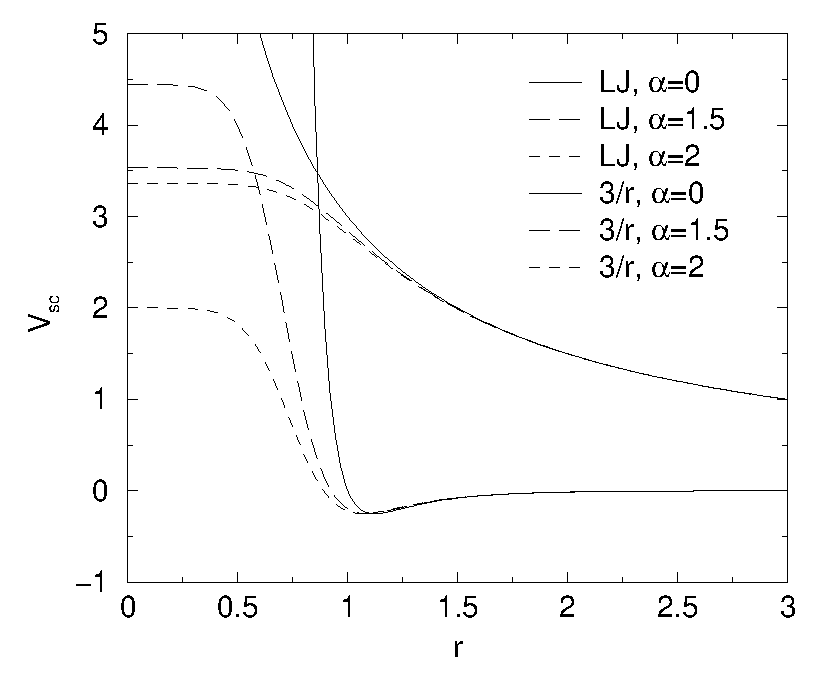
\includegraphics[height=6cm]{plots/softcore}}
\caption{Soft-core interactions at $\LAM=0.5$, with $p=2$ and
$C_6^A=C_{12}^A=C_6^B=C_{12}^B=1$.}
\label{fig:softcore}
\end{figure}
In a free-energy calculation where particles grow out of nothing, or 
particles disappear, using the the simple linear interpolation of the 
Lennard-Jones and Coulomb potentials as described in Equations~\ref{eq:dVljdlambda}
and \ref{eq:dVcoulombdlambda} may lead to poor convergence.  When the particles have nearly disappeared, or are close to appearing (at $\LAM$ close to 0 or 1), the interaction energy will be weak enough for particles to get very 
close to each other, leading to large fluctuations in the measured values of 
$\partial V/\partial \LAM$ (which, because of the simple linear 
interpolation, depends on the potentials at both the endpoints of $\LAM$).

To circumvent these problems, the singularities in the potentials need to be removed. This can be done by modifying the regular Lennard-Jones and Coulomb potentials with ``soft-core'' potentials that limit the energies and forces 
involved at $\LAM$ values between 0 and 1, but not \emph{at} $\LAM=0$ 
or 1.

In {\gromacs} the soft-core potentials $V_{sc}$ are shifted versions of the
regular potentials, so that the singularity in the potential and its
derivatives at $r=0$ is never reached:
\bea
V_{sc}(r) &=& \LL V^A(r_A) + \LAM V^B(r_B)
    \\
r_A &=& \left(\alpha \sigma_A^6 \LAM^p + r^6 \right)^\frac{1}{6}
    \\
r_B &=& \left(\alpha \sigma_B^6 \LL^p + r^6 \right)^\frac{1}{6}
\eea
where $V^A$ and $V^B$ are the normal ``hard core'' Van der Waals or
electrostatic potentials in state A ($\LAM=0$) and state B ($\LAM=1$)
respectively, $\alpha$ is the soft-core parameter (set with {\tt sc_alpha} 
in the {\tt .mdp} file), $p$ is the soft-core $\LAM$ power (set with 
{\tt sc_power}), $\sigma$ is the radius of the interaction, which is 
$(C_{12}/C_6)^{1/6}$ or an input parameter ({\tt sc_sigma}) when $C_6$ 
or $C_{12}$ is zero.

For intermediate $\LAM$, $r_A$ and $r_B$ alter the interactions very little
for $r > \alpha^{1/6} \sigma$ and quickly switch the soft-core
interaction to an almost constant value for smaller $r$ (\figref{softcore}). 
The force is:
\beq
F_{sc}(r) = -\frac{\partial V_{sc}(r)}{\partial r} =
 \LL F^A(r_A) \left(\frac{r}{r_A}\right)^5 +
\LAM F^B(r_B) \left(\frac{r}{r_B}\right)^5
\eeq
where $F^A$ and $F^B$ are the ``hard core'' forces.
The contribution to the derivative of the free energy is:
\bea
\dvdl{V_{sc}(r)} & = &
 V^B(r_B) -V^A(r_A)  + 
	\LL \frac{\partial V^A(r_A)}{\partial r_A}
		   \frac{\partial r_A}{\partial \LAM} + 
	\LAM\frac{\partial V^B(r_B)}{\partial r_B}
		   \frac{\partial r_B}{\partial \LAM}
\nonumber\\
&=&
 V^B(r_B) -V^A(r_A)  + \nonumber \\
 & &
 \frac{p \alpha}{6}
       \left[ \LAM F^B(r_B) r^{-5}_B \sigma_B^6 \LL^{p-1} -
	       \LL F^A(r_A) r^{-5}_A \sigma_A^6 \LAM^{p-1} \right]
\eea

The original GROMOS Lennard-Jones soft-core function~\cite{Beutler94}
uses $p=2$, but $p=1$ gives a smoother $\partial H/\partial\LAM$ curve.
%When the changes between the two states involve both the disappearing
%and appearing of atoms, it is important that the overlapping of atoms
%happens around $\LAM=0.5$. This can usually be achieved with
%$\alpha$$\approx0.7$ for $p=1$ and $\alpha$$\approx1.5$ for $p=2$.
%MRS: this is now eliminated as of 4.6, since changes between atoms are done linearly.

Another issue that should be considered is the soft-core effect of hydrogens
without Lennard-Jones interaction. Their soft-core $\sigma$ is
set with {\tt sc-sigma} in the {\tt .mdp} file. These hydrogens
produce peaks in $\partial H/\partial\LAM$ at $\LAM$ is 0 and/or 1 for $p=1$
and close to 0 and/or 1 with $p=2$. Lowering {\tt\mbox{sc-sigma}} will decrease
this effect, but it will also increase the interactions with hydrogens
relative to the other interactions in the soft-core state.

When soft-core potentials are selected (by setting {\tt sc-alpha} \textgreater
0), and the Coulomb and Lennard-Jones potentials are turned on or off
sequentially, then the Coulombic interaction is turned off linearly,
rather than using soft-core interactions, which should be less
statistically noisy in most cases. This behavior can be overwritten
by using the mdp option {\tt sc-coul} to {\tt yes}. Note that the {\tt sc-coul}
is only taken into account when lambda states are used, not with
{\tt couple-lambda0}~/ {\tt couple-lambda1}, and you can still turn off soft-core
interactions by setting {\tt sc-alpha=0}. Additionally, the soft-core
interaction potential is only applied when either the A or B
state has zero interaction potential. If both A and B states have
nonzero interaction potential, default linear scaling described above
is used. When both Coulombic and Lennard-Jones interactions are turned
off simultaneously, a soft-core potential is used, and a hydrogen is
being introduced or deleted, the sigma is set to {\tt sc-sigma-min},
which itself defaults to {\tt sc-sigma-default}.

Recently, a new formulation of the soft-core approach has been derived
that in most cases gives lower and more even statistical variance than
the standard soft-core path described above.~\cite{Pham2011,Pham2012}
Specifically, we have:
\bea
V_{sc}(r) &=& \LL V^A(r_A) + \LAM V^B(r_B)
    \\
r_A &=& \left(\alpha \sigma_A^{48} \LAM^p + r^{48} \right)^\frac{1}{48}
    \\
r_B &=& \left(\alpha \sigma_B^{48} \LL^p + r^{48} \right)^\frac{1}{48}
\eea
This ``1-1-48'' path is also implemented in {\gromacs}. Note that for this path the soft core $\alpha$
should satisfy $0.001 < \alpha < 0.003$, rather than $\alpha \approx
0.5$.

%} % Brace matches ifthenelse test for gmxlite

%\ifthenelse{\equal{\gmxlite}{1}}{}{
\section{Methods}
\subsection{Exclusions and 1-4 Interactions.}
Atoms within a molecule that are close by in the chain, 
{\ie} atoms that are covalently bonded, or linked by one or two
atoms are called {\em first neighbors, second neighbors} and 
{\em \swapindex{third}{neighbor}s}, respectively (see \figref{chain}).  
Since the interactions of atom {\bf i} with atoms {\bf i+1} and {\bf i+2} 
are mainly quantum mechanical, they can not be modeled by a Lennard-Jones potential.
Instead it is assumed that these interactions are adequately modeled
by a harmonic bond term or constraint ({\bf i, i+1}) and a harmonic angle term
({\bf i, i+2}). The first and second neighbors (atoms {\bf i+1} and {\bf i+2}) 
are therefore
{\em excluded} from the Lennard-Jones \swapindex{interaction}{list} 
of atom {\bf i};
atoms {\bf i+1} and {\bf i+2} are called {\em \normindex{exclusions}} of atom {\bf i}.

\begin{figure}
\centerline{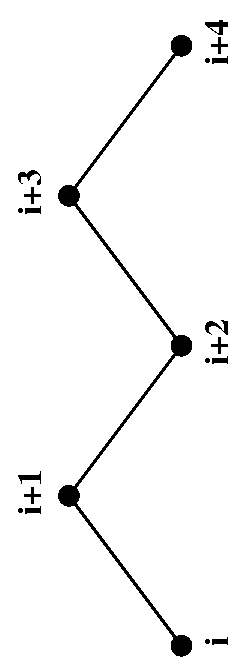
\includegraphics[width=8cm]{plots/chain}}
\caption{Atoms along an alkane chain.}
\label{fig:chain}
\end{figure}

For third neighbors, the normal Lennard-Jones repulsion is sometimes
still too strong, which means that when applied to a molecule, the
molecule would deform or break due to the internal strain. This is
especially the case for carbon-carbon interactions in a {\em
cis}-conformation ({\eg} {\em cis}-butane).  Therefore, for some of these
interactions, the Lennard-Jones repulsion has been reduced in the
{\gromos} force field, which is implemented by keeping a separate list of
1-4 and normal Lennard-Jones parameters. In other force fields, such
as OPLS~\cite{Jorgensen88}, the standard Lennard-Jones parameters are reduced
by a factor of two, but in that case also the dispersion (r$^{-6}$)
and the Coulomb interaction are scaled.
{\gromacs} can use either of these methods.

\subsection{Charge Groups\index{charge group}}
\label{sec:cg}
In principle, the force calculation in MD is an $O(N^2)$ problem.
Therefore, we apply a \normindex{cut-off} for non-bonded force (NBF)
calculations; only the particles within a certain distance of each
other are interacting. This reduces the cost to $O(N)$ (typically
$100N$ to $200N$) of the NBF. It also introduces an error, which is,
in most cases, acceptable, except when applying the cut-off implies
the creation of charges, in which case you should consider using the
lattice sum methods provided by {\gromacs}.

Consider a water molecule interacting with another atom. If we would apply
a plain cut-off on an atom-atom basis we might include the atom-oxygen
interaction (with a charge of $-0.82$) without the compensating charge
of the protons, and as a result, induce a large dipole moment over the system.
Therefore, we have to keep groups of atoms with total charge
0 together. These groups are called {\em charge groups}. Note that with
a proper treatment of long-range electrostatics (e.g. particle-mesh Ewald
(\secref{pme}), keeping charge groups together is not required.

\subsection{Treatment of Cut-offs in the group scheme\index{cut-off}}
\newcommand{\rs}{$r_{short}$}
\newcommand{\rl}{$r_{long}$}
{\gromacs} is quite flexible in treating cut-offs, which implies
there can be quite a number of parameters to set. These parameters are
set in the input file for {\tt grompp}. There are two sort of parameters
that affect the cut-off interactions; you can select which type
of interaction to use in each case, and which cut-offs should be
used in the neighbor searching.

For both Coulomb and van der Waals interactions there are interaction
type selectors (termed {\tt vdwtype} and {\tt coulombtype}) and two
parameters, for a total of six non-bonded interaction parameters. See
the User Guide for a complete description of these parameters.

In the group cut-off scheme, all of the interaction functions in \tabref{funcparm}
require that neighbor searching be done with a radius at least as large as the $r_c$
specified for the functional form, because of the use of charge groups.
The extra radius is typically of the order of 0.25 nm (roughly the 
largest distance between two atoms in a charge group plus the distance a 
charge group can diffuse within neighbor list updates).

\begin{table}[ht]
\centering
\begin{tabular}{|ll|l|}
\dline
\multicolumn{2}{|c|}{Type}              & Parameters            \\
\hline
Coulomb&Plain cut-off   & $r_c$, $\epsr$        \\
&Reaction field         & $r_c$, $\epsrf$       \\
&Shift function         & $r_1$, $r_c$, $\epsr$         \\
&Switch function        & $r_1$, $r_c$, $\epsr$         \\
\hline
VdW&Plain cut-off       & $r_c$         \\
&Shift function         & $r_1$, $r_c$          \\
&Switch function        & $r_1$, $r_c$          \\
\dline
\end{tabular}
\caption[Parameters for the different functional forms of the
non-bonded interactions.]{Parameters for the different functional
forms of the non-bonded interactions.}
\label{tab:funcparm}
\end{table}
%} % Brace matches ifthenelse test for gmxlite


\newcommand{\vvis}{\ve{r}_s}
\newcommand{\Fi}{\ve{F}_i'}
\newcommand{\Fj}{\ve{F}_j'}
\newcommand{\Fk}{\ve{F}_k'}
\newcommand{\Fl}{\ve{F}_l'}
\newcommand{\Fvis}{\ve{F}_{s}}
\newcommand{\rvik}{\ve{r}_{ik}}
\newcommand{\rvis}{\ve{r}_{is}}
\newcommand{\rvjk}{\ve{r}_{jk}}
\newcommand{\rvjl}{\ve{r}_{jl}}

%\ifthenelse{\equal{\gmxlite}{1}}{}{
\section{Virtual interaction sites\index{virtual interaction sites}}
\label{sec:virtual_sites}
Virtual interaction sites (called \seeindex{dummy atoms}{virtual interaction sites} in {\gromacs} versions before 3.3)
can be used in {\gromacs} in a number of ways. 
We write the position of the virtual site $\ve{r}_s$ as a function of
the positions of other particles \ve{r}$_i$: $\ve{r}_s =
f(\ve{r}_1..\ve{r}_n)$. The virtual site, which may carry charge or be
involved in other interactions, can now be used in the force
calculation.  The force acting on the virtual site must be
redistributed over the particles with mass in a consistent way.
A good way to do this can be found in ref.~\cite{Berendsen84b}.
We can write the potential energy as:
\beq
V = V(\vvis,\ve{r}_1,\ldots,\ve{r}_n) = V^*(\ve{r}_1,\ldots,\ve{r}_n)
\eeq
The force on the particle $i$ is then:
\beq
\ve{F}_i = -\frac{\partial V^*}{\partial \ve{r}_i} 
         = -\frac{\partial V}{\partial \ve{r}_i} - 
            \frac{\partial V}{\partial \vvis} 
            \frac{\partial \vvis}{\partial \ve{r}_i}
         = \ve{F}_i^{direct} + \Fi
\eeq
The first term is the normal force. 
The second term is the force on particle $i$ due to the virtual site, which
can be written in tensor notation:
\newcommand{\partd}[2]{\displaystyle\frac{\partial #1}{\partial #2_i}}
\beq
\Fi = \left[\begin{array}{ccc}
\partd{x_s}{x} & \partd{y_s}{x} & \partd{z_s}{x}        \\[1ex]
\partd{x_s}{y} & \partd{y_s}{y} & \partd{z_s}{y}        \\[1ex]
\partd{x_s}{z} & \partd{y_s}{z} & \partd{z_s}{z}
\end{array}\right]\Fvis
\label{eqn:fvsite}
\eeq
where $\Fvis$ is the force on the virtual site and $x_s$, $y_s$ and
$z_s$ are the coordinates of the virtual site. In this way, the total
force and the total torque are conserved~\cite{Berendsen84b}.

The computation of the \normindex{virial}
(\eqnref{Xi}) is non-trivial when virtual sites are used. Since the
virial involves a summation over all the atoms (rather than virtual
sites), the forces must be redistributed from the virtual sites to the
atoms (using ~\eqnref{fvsite}) {\em before} computation of the
virial. In some special cases where the forces on the atoms can be
written as a linear combination of the forces on the virtual sites (types 2
and 3 below) there is no difference between computing the virial
before and after the redistribution of forces.  However, in the
general case redistribution should be done first.

\begin{figure}
\centerline{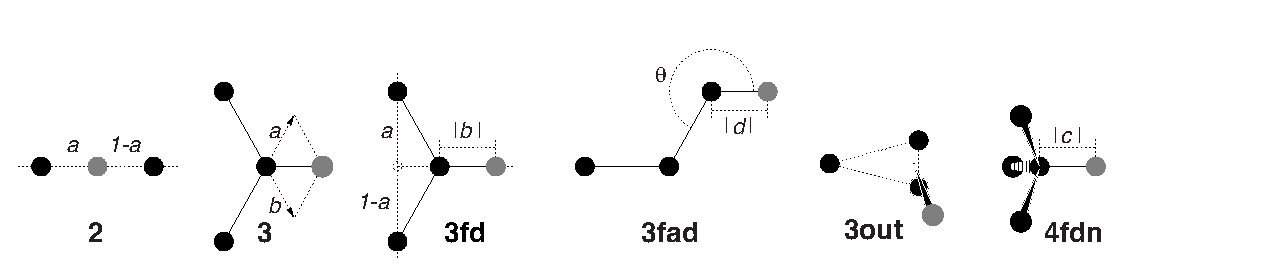
\includegraphics[width=15cm]{plots/dummies}}
\caption[Virtual site construction.]{The six different types of virtual
site construction in \protect{\gromacs}. The constructing atoms are
shown as black circles, the virtual sites in gray.}
\label{fig:vsites}
\end{figure}

There are six ways to construct virtual sites from surrounding atoms in
{\gromacs}, which we classify by the number of constructing
atoms. {\bf Note} that all site types mentioned can be constructed from
types 3fd (normalized, in-plane) and 3out (non-normalized, out of
plane). However, the amount of computation involved increases sharply
along this list, so we strongly recommended using the first adequate
virtual site type that will be sufficient for a certain purpose.
\figref{vsites} depicts 6 of the available virtual site constructions.
The conceptually simplest construction types are linear combinations:
\beq
\vvis = \sum_{i=1}^N w_i \, \ve{r}_i
\eeq
The force is then redistributed using the same weights:
\beq
\Fi = w_i \, \Fvis
\eeq

The types of virtual sites supported in {\gromacs} are given in the list below.
Constructing atoms in virtual sites can be virtual sites themselves, but
only if they are higher in the list, i.e. virtual sites can be
constructed from ``particles'' that are simpler virtual sites.
\begin{itemize}
\item[{\bf\sf 2.}]\label{subsec:vsite2}As a linear combination of two atoms
        (\figref{vsites} 2):
\beq
        w_i = 1 - a ~,~~ w_j = a
\eeq
        In this case the virtual site is on the line through atoms $i$ and
        $j$.

\item[{\bf\sf 3.}]\label{subsec:vsite3}As a linear combination of three atoms
        (\figref{vsites} 3):
\beq
        w_i = 1 - a - b ~,~~ w_j = a ~,~~ w_k = b
\eeq
        In this case the virtual site is in the plane of the other three
	particles.

\item[{\bf\sf 3fd.}]\label{subsec:vsite3fd}In the plane of three atoms, with a fixed distance
        (\figref{vsites} 3fd):
\beq
        \vvis ~=~ \ve{r}_i + b \frac{  \rvij + a \rvjk  }
                                    {| \rvij + a \rvjk |}      
\eeq
        In this case the virtual site is in the plane of the other three
        particles at a distance of $|b|$ from $i$.
        The force on particles $i$, $j$ and $k$ due to the force on the virtual
        site can be computed as:
\beq
        \begin{array}{lcr}
        \Fi &=& \displaystyle \Fvis - \gamma ( \Fvis - \ve{p} ) \\[1ex]
        \Fj &=& \displaystyle (1-a)\gamma (\Fvis - \ve{p})      \\[1ex]
        \Fk &=& \displaystyle a \gamma (\Fvis - \ve{p})         \\
        \end{array}
        ~\mbox{~ where~ }~
        \begin{array}{c}
\displaystyle \gamma = \frac{b}{| \rvij + a \rvjk |} \\[2ex]
\displaystyle \ve{p} = \frac{ \rvis \cdot \Fvis }
                      { \rvis \cdot \rvis } \rvis
        \end{array}
\eeq

\item[{\bf\sf 3fad.}]\label{subsec:vsite3fad}In the plane of three atoms, with a fixed angle and
        distance (\figref{vsites} 3fad):
\beq
\label{eqn:vsite2fad-F}
         \vvis ~=~ \ve{r}_i +
                    d \cos \theta \frac{\rvij}{|\rvij|} +
                    d \sin \theta \frac{\ve{r}_\perp}{|\ve{r}_\perp|}
        ~\mbox{~ where~ }~
        \ve{r}_\perp ~=~ \rvjk - 
                        \frac{ \rvij \cdot \rvjk }
                             { \rvij \cdot \rvij }
                         \rvij
\eeq
        In this case the virtual site is in the plane of the other three
        particles at a distance of $|d|$ from $i$ at an angle of
        $\alpha$ with $\rvij$. Atom $k$ defines the plane and the
        direction of the angle. {\bf Note} that in this case $b$ and
        $\alpha$ must be specified, instead of $a$ and $b$ (see also
        \secref{vsitetop}). The force on particles $i$, $j$ and $k$
        due to the force on the virtual site can be computed as (with
        $\ve{r}_\perp$ as defined in \eqnref{vsite2fad-F}):
\newcommand{\dfrac}{\displaystyle\frac}
\beq
\begin{array}{c}
        \begin{array}{lclllll}
        \Fi &=& \Fvis &-& 
                \dfrac{d \cos \theta}{|\rvij|} \ve{F}_1 &+&
                \dfrac{d \sin \theta}{|\ve{r}_\perp|} \left( 
                \dfrac{ \rvij \cdot \rvjk }
                     { \rvij \cdot \rvij } \ve{F}_2     +
                \ve{F}_3 \right)                                \\[3ex]
        \Fj &=& &&
                \dfrac{d \cos \theta}{|\rvij|} \ve{F}_1 &-&
                \dfrac{d \sin \theta}{|\ve{r}_\perp|} \left(
                 \ve{F}_2 + 
                 \dfrac{ \rvij \cdot \rvjk }
                        { \rvij \cdot \rvij } \ve{F}_2 +
                \ve{F}_3 \right)                                \\[3ex]
        \Fk &=& && &&
                \dfrac{d \sin \theta}{|\ve{r}_\perp|} \ve{F}_2  \\[3ex]
        \end{array}                                             \\[5ex]
        \mbox{where ~}
        \ve{F}_1 = \Fvis -
                  \dfrac{ \rvij \cdot \Fvis }
                        { \rvij \cdot \rvij } \rvij
        \mbox{\,, ~}
        \ve{F}_2 = \ve{F}_1 -
                  \dfrac{ \ve{r}_\perp \cdot \Fvis }
                        { \ve{r}_\perp \cdot \ve{r}_\perp } \ve{r}_\perp
        \mbox{~and ~}
        \ve{F}_3 = \dfrac{ \rvij \cdot \Fvis }
                         { \rvij \cdot \rvij } \ve{r}_\perp
\end{array}
\eeq

\item[{\bf\sf 3out.}]\label{subsec:vsite3out}As a non-linear combination of three atoms, out of plane
        (\figref{vsites} 3out):
\beq
        \vvis ~=~ \ve{r}_i + a \rvij + b \rvik +
                c (\rvij \times \rvik)
\eeq
        This enables the construction of virtual sites out of the plane of the
        other atoms.
        The force on particles $i,j$ and $k$ due to the force on the virtual
        site can be computed as:
\beq
\begin{array}{lcl}
\vspace{4mm}
\Fj &=& \left[\begin{array}{ccc}
 a              &  -c\,z_{ik}   & c\,y_{ik}     \\[0.5ex]
 c\,z_{ik}      &   a           & -c\,x_{ik}    \\[0.5ex]
-c\,y_{ik}      &   c\,x_{ik}   & a
\end{array}\right]\Fvis                                 \\
\vspace{4mm}
\Fk &=& \left[\begin{array}{ccc}
 b              &   c\,z_{ij}   & -c\,y_{ij}    \\[0.5ex]
-c\,z_{ij}      &   b           & c\,x_{ij}     \\[0.5ex]
 c\,y_{ij}      &  -c\,x_{ij}   & b
\end{array}\right]\Fvis                                 \\
\Fi &=& \Fvis - \Fj - \Fk
\end{array}
\eeq

\item[{\bf\sf 4fdn.}]\label{subsec:vsite4fdn}From four atoms, with a fixed distance, see separate Fig.\ \ref{fig:vsite-4fdn}.
This construction is a bit
complex, in particular since the previous type (4fd) could be unstable which forced us
to introduce a more elaborate construction:

\begin{figure}
\centerline{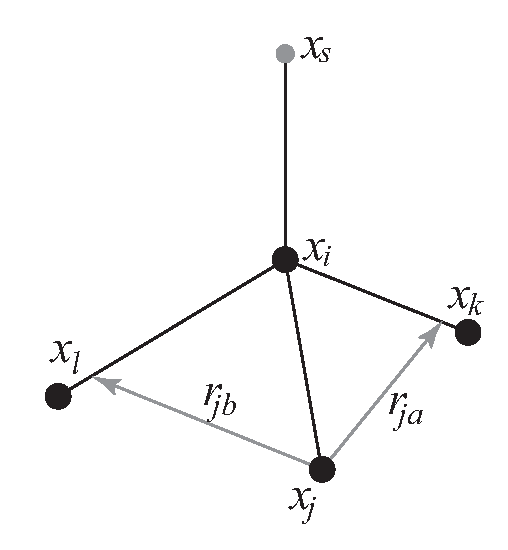
\includegraphics[width=5cm]{plots/vsite-4fdn}}
\caption {The new 4fdn virtual site construction, which is stable even when all constructing
atoms are in the same plane.}
\label{fig:vsite-4fdn}
\end{figure}
         
\begin{eqnarray}
\mathbf{r}_{ja} &=& a\, \mathbf{r}_{ik} - \mathbf{r}_{ij} = a\, (\mathbf{x}_k - \mathbf{x}_i) - (\mathbf{x}_j - \mathbf{x}_i) \nonumber \\
\mathbf{r}_{jb} &=& b\, \mathbf{r}_{il} - \mathbf{r}_{ij} = b\, (\mathbf{x}_l - \mathbf{x}_i) - (\mathbf{x}_j - \mathbf{x}_i) \nonumber \\
\mathbf{r}_m &=& \mathbf{r}_{ja} \times \mathbf{r}_{jb} \nonumber \\
\mathbf{x}_s &=& \mathbf{x}_i + c \frac{\mathbf{r}_m}{|\mathbf{r}_m|}
\label{eq:vsite}
\end{eqnarray}

        In this case the virtual site is at a distance of $|c|$ from $i$, while $a$ and $b$ are 
        parameters. {\bf Note} that the vectors $\mathbf{r}_{ik}$ and $\mathbf{r}_{ij}$ are not normalized
        to save floating-point operations.
        The force on particles $i$, $j$, $k$ and $l$ due to the force 
        on the virtual site are computed through chain rule derivatives
        of the construction expression. This is exact and conserves energy,
        but it does lead to relatively lengthy expressions that we do not
        include here (over 200 floating-point operations). The interested reader can 
        look at the source code in \verb+vsite.c+. Fortunately, this vsite type is normally
        only used for chiral centers such as $C_{\alpha}$ atoms in proteins.
      
The new 4fdn construct is identified with a `type' value of 2 in the topology. The earlier 4fd
type is still supported internally (`type' value 1), but it should not be used for
new simulations. All current {\gromacs} tools will automatically generate type 4fdn instead.


\item[{\bf\sf N.}]\label{subsec:vsiteN} A linear combination of $N$ atoms with relative
weights $a_i$. The weight for atom $i$ is:
\beq
  w_i = a_i \left(\sum_{j=1}^N a_j \right)^{-1}
\eeq
There are three options for setting the weights:
\begin{itemize}
\item[COG] center of geometry: equal weights
\item[COM] center of mass: $a_i$ is the mass of atom $i$;
when in free-energy simulations the mass of the atom is changed,
only the mass of the A-state is used for the weight
\item[COW] center of weights: $a_i$ is defined by the user
\end{itemize}

\end{itemize}
%} % Brace matches ifthenelse test for gmxlite

\newcommand{\dr}{{\rm d}r}
\newcommand{\avcsix}{\left< C_6 \right>}

%\ifthenelse{\equal{\gmxlite}{1}}{}{
\section{Long Range Electrostatics}
\label{sec:lr_elstat}
\subsection{Ewald summation\index{Ewald sum}}
\label{sec:ewald}
The total electrostatic energy of $N$ particles and their periodic
images\index{periodic boundary conditions} is given by
\begin{equation}
V=\frac{f}{2}\sum_{n_x}\sum_{n_y}
\sum_{n_{z}*} \sum_{i}^{N} \sum_{j}^{N}
\frac{q_i q_j}{{\bf r}_{ij,{\bf n}}}.
\label{eqn:totalcoulomb}
\end{equation}
$(n_x,n_y,n_z)={\bf n}$ is the box index vector, and the star indicates that
terms with $i=j$ should be omitted when $(n_x,n_y,n_z)=(0,0,0)$. The
distance ${\bf r}_{ij,{\bf n}}$ is the real distance between the charges and
not the minimum-image. This sum is conditionally convergent, but
very slow.

Ewald summation was first introduced as a method to calculate
long-range interactions of the periodic images in
crystals~\cite{Ewald21}. The idea is to convert the single
slowly-converging sum \eqnref{totalcoulomb} into two
quickly-converging terms and a constant term:
\begin{eqnarray}
V &=& V_{\mathrm{dir}} + V_{\mathrm{rec}} + V_{0} \\[0.5ex]
V_{\mathrm{dir}} &=& \frac{f}{2} \sum_{i,j}^{N}
\sum_{n_x}\sum_{n_y}
\sum_{n_{z}*} q_i q_j \frac{\mbox{erfc}(\beta {r}_{ij,{\bf n}} )}{{r}_{ij,{\bf n}}} \\[0.5ex]
V_{\mathrm{rec}} &=& \frac{f}{2 \pi V} \sum_{i,j}^{N} q_i q_j
\sum_{m_x}\sum_{m_y}
\sum_{m_{z}*} \frac{\exp{\left( -(\pi {\bf m}/\beta)^2 + 2 \pi i
      {\bf m} \cdot ({\bf r}_i - {\bf r}_j)\right)}}{{\bf m}^2} \\[0.5ex]
V_{0} &=& -\frac{f \beta}{\sqrt{\pi}}\sum_{i}^{N} q_i^2,
\end{eqnarray}
where $\beta$ is a parameter that determines the relative weight of the
direct and reciprocal sums and ${\bf m}=(m_x,m_y,m_z)$.
In this way we can use a short cut-off (of the order of $1$~nm) in the direct space sum and a
short cut-off in the reciprocal space sum ({\eg} 10 wave vectors in each
direction). Unfortunately, the computational cost of the reciprocal
part of the sum increases as $N^2$
(or $N^{3/2}$ with a slightly better algorithm) and it is therefore not
realistic for use in large systems.

\subsubsection{Using Ewald}
Don't use Ewald unless you are absolutely sure this is what you want -
for almost all cases the PME method below will perform much better.
If you still want to employ classical Ewald summation enter this in
your {\tt .mdp} file, if the side of your box is about $3$~nm:

\begin{verbatim}
coulombtype     = Ewald
rvdw            = 0.9
rlist           = 0.9
rcoulomb        = 0.9
fourierspacing  = 0.6
ewald-rtol      = 1e-5
\end{verbatim}

The ratio of the box dimensions and the {\tt fourierspacing} parameter determines
the highest magnitude of wave vectors $m_x,m_y,m_z$ to use in each
direction. With a 3-nm cubic box this example would use $11$ wave vectors
(from $-5$ to $5$) in each direction.  The {\tt ewald-rtol} parameter
is the relative strength of the electrostatic interaction at the
cut-off. Decreasing this gives you a more accurate direct sum, but a
less accurate reciprocal sum.

\subsection{\normindex{PME}}
\label{sec:pme}
Particle-mesh Ewald is a method proposed by Tom
Darden~\cite{Darden93} to improve the performance of the
reciprocal sum. Instead of directly summing wave vectors, the charges
are assigned to a grid using interpolation. The implementation in
{\gromacs} uses cardinal B-spline interpolation~\cite{Essmann95},
which is referred to as smooth PME (SPME).
The grid is then Fourier transformed with a 3D FFT algorithm and the
reciprocal energy term obtained by a single sum over the grid in
k-space.

The potential at the grid points is calculated by inverse
transformation, and by using the interpolation factors we get the
forces on each atom.

The PME algorithm scales as $N \log(N)$, and is substantially faster
than ordinary Ewald summation on medium to large systems. On very
small systems it might still be better to use Ewald to avoid the
overhead in setting up grids and transforms.
For the parallelization of PME see the section on MPMD PME (\ssecref{mpmd_pme}).

With the Verlet cut-off scheme, the PME direct space potential is
shifted by a constant such that the potential is zero at the
cut-off. This shift is small and since the net system charge is close
to zero, the total shift is very small, unlike in the case of the
Lennard-Jones potential where all shifts add up. We apply the shift
anyhow, such that the potential is the exact integral of the force.

\subsubsection{Using PME}
As an example for using Particle-mesh Ewald summation in {\gromacs}, specify the
following lines in your {\tt .mdp} file:

\begin{verbatim}
coulombtype     = PME
rvdw            = 0.9
rlist           = 0.9
rcoulomb        = 0.9
fourierspacing  = 0.12
pme-order       = 4
ewald-rtol      = 1e-5
\end{verbatim}

In this case the {\tt fourierspacing} parameter determines the maximum
spacing for the FFT grid (i.e. minimum number of grid points),
and {\tt pme-order} controls the
interpolation order. Using fourth-order (cubic) interpolation and this
spacing should give electrostatic energies accurate to about
$5\cdot10^{-3}$. Since the Lennard-Jones energies are not this
accurate it might even be possible to increase this spacing slightly.

Pressure scaling works with PME, but be aware of the fact that
anisotropic scaling can introduce artificial ordering in some systems.

\subsection{\normindex{P3M-AD}}
\label{sec:pppm}
The \seeindex{Particle-Particle Particle-Mesh}{P3M} methods of
Hockney \& Eastwood can also be applied in {\gromacs} for the
treatment of long range electrostatic interactions~\cite{Hockney81}.
Although the P3M method was the first efficient long-range electrostatics
method for molecular simulation, the smooth PME (SPME) method has largely
replaced P3M as the method of choice in atomistic simulations. One performance
disadvantage of the original P3M method was that it required 3 3D-FFT
back transforms to obtain the forces on the particles. But this is not
required for P3M and the forces can be derived through analytical differentiation
of the potential, as done in PME. The resulting method is termed P3M-AD.
The only remaining difference between P3M-AD and PME is the optimization
of the lattice Green influence function for error minimization that P3M uses.
However, in 2012 it has been shown that the SPME influence function can be
modified to obtain P3M~\cite{Ballenegger2012}.
This means that the advantage of error minimization in P3M-AD can be used
at the same computational cost and with the same code as PME,
just by adding a few lines to modify the influence function.
However, at optimal parameter setting the effect of error minimization
in P3M-AD is less than 10\%. P3M-AD does show large accuracy gains with
interlaced (also known as staggered) grids, but that is not supported
in {\gromacs} (yet).

P3M is used in {\gromacs} with exactly the same options as used with PME
by selecting the electrostatics type:
\begin{verbatim}
coulombtype     = P3M-AD
\end{verbatim}

\subsection{Optimizing Fourier transforms and PME calculations}
It is recommended to optimize the parameters for calculation of
electrostatic interaction such as PME grid dimensions and cut-off radii.
This is particularly relevant to do before launching long production runs.

{\tt gmx mdrun} will automatically do a lot of PME optimization, and
{\gromacs} also includes a special tool, {\tt gmx tune_pme}, which
automates the process of selecting the optimal number of PME-only ranks.

%%%%%%%%%%%%%%%%%%%%%%%%%%%%%%%%%%%%%%%%%%%%%%%%%%%%%%%%%%%%%%%%%%%
%%%%%%%%%%%%%%%%%%%%%%%%%%%%%%%%%%%%%%%%%%%%%%%%%%%%%%%%%%%%%%%%%%%
%%%%%%%%%%%%%%%%%%%%%%%%%%%%%%%%%%%%%%%%%%%%%%%%%%%%%%%%%%%%%%%%%%%

%\ifthenelse{\equal{\gmxlite}{1}}{}{
\section{Long Range Van der Waals interactions}
\subsection{Dispersion correction\index{dispersion correction}}
In this section, we derive long-range corrections due to the use of a
cut-off for Lennard-Jones or Buckingham interactions.
We assume that the cut-off is
so long that the repulsion term can safely be neglected, and therefore
only the dispersion term is taken into account. Due to the nature of
the dispersion interaction (we are truncating a potential proportional
to $-r^{-6}$), energy and pressure corrections are both negative. While
the energy correction is usually small, it may be important for free
energy calculations where differences between two different Hamiltonians
are considered. In contrast, the pressure correction is very large and
can not be neglected under any circumstances where a correct pressure is
required, especially for any NPT simulations. Although it is, in
principle, possible to parameterize a force field such that the pressure
is close to the desired experimental value without correction, such a
method makes the parameterization dependent on the cut-off and is therefore
undesirable.

\subsubsection{Energy}
\label{sec:ecorr}
The long-range contribution of the dispersion interaction to the
virial can be derived analytically, if we assume a homogeneous
system beyond the cut-off distance $r_c$. The dispersion energy
between two particles is written as:
\beq
V(\rij) ~=~- C_6\,\rij^{-6}
\eeq
and the corresponding force is:
\beq
\Fvij ~=~- 6\,C_6\,\rij^{-8}\rvij
\eeq
In a periodic system it is not easy to calculate the full potentials,
so usually a cut-off is applied, which can be abrupt or smooth.
We will call the potential and force with cut-off $V_c$ and $\ve{F}_c$.
The long-range contribution to the dispersion energy
in a system with $N$ particles and particle density $\rho$ = $N/V$ is:
\beq
\label{eqn:enercorr}
V_{lr} ~=~ \half N \rho\int_0^{\infty}   4\pi r^2 g(r) \left( V(r) -V_c(r) \right) {\dr}
\eeq
We will integrate this for the shift function, which is the most general
form of van der Waals interaction available in {\gromacs}.
The shift function has a constant difference $S$ from 0 to $r_1$
and is 0 beyond the cut-off distance $r_c$.
We can integrate \eqnref{enercorr}, assuming that the density in the sphere
within $r_1$ is equal to the global density and
the radial distribution function $g(r)$ is 1 beyond $r_1$:
\bea
\nonumber
V_{lr}  &=& \half N \left(
  \rho\int_0^{r_1}  4\pi r^2 g(r) \, C_6 \,S\,{\dr}
+ \rho\int_{r_1}^{r_c}  4\pi r^2 \left( V(r) -V_c(r) \right) {\dr}
+ \rho\int_{r_c}^{\infty}  4\pi r^2 V(r) \, {\dr}
\right) \\
& = & \half N \left(\left(\frac{4}{3}\pi \rho r_1^{3} - 1\right) C_6 \,S
+ \rho\int_{r_1}^{r_c} 4\pi r^2 \left( V(r) -V_c(r) \right) {\dr}
-\frac{4}{3} \pi N \rho\, C_6\,r_c^{-3}
\right)
\eea
where the term $-1$ corrects for the self-interaction.
For a plain cut-off we only need to assume that $g(r)$ is 1 beyond $r_c$
and the correction reduces to~\cite{Allen87}:
\bea
V_{lr} & = & -\frac{2}{3} \pi N \rho\, C_6\,r_c^{-3}
\eea
If we consider, for example, a box of pure water, simulated with a cut-off
of 0.9 nm and a density of 1 g cm$^{-3}$ this correction is
$-0.75$ kJ mol$^{-1}$ per molecule.

For a homogeneous mixture we need to define
an {\em average dispersion constant}:
\beq
\label{eqn:avcsix}
\avcsix	= \frac{2}{N(N-1)}\sum_i^N\sum_{j>i}^N C_6(i,j)\\
\eeq
In {\gromacs}, excluded pairs of atoms do not contribute to the average.

In the case of inhomogeneous simulation systems, {\eg} a system with a
lipid interface, the energy correction can be applied if
$\avcsix$ for both components is comparable.

\subsubsection{Virial and pressure}
The scalar virial of the system due to the dispersion interaction between
two particles $i$ and $j$ is given by:
\beq
\Xi~=~-\half \rvij \cdot \Fvij ~=~ 3\,C_6\,\rij^{-6}
\eeq
The pressure is given by:
\beq
P~=~\frac{2}{3\,V}\left(E_{kin} - \Xi\right)
\eeq
The long-range correction to the virial is given by:
\beq
\Xi_{lr} ~=~ \half N \rho \int_0^{\infty} 4\pi r^2 g(r) (\Xi -\Xi_c) \,\dr
\eeq
We can again integrate the long-range contribution to the
virial assuming $g(r)$ is 1 beyond $r_1$:
\bea
\Xi_{lr}&=&	\half N \rho \left(
    \int_{r_1}^{r_c}  4 \pi r^2 (\Xi -\Xi_c)  \,\dr
  + \int_{r_c}^{\infty} 4 \pi r^2 3\,C_6\,\rij^{-6}\,  \dr
\right)	\nonumber\\
        &=&     \half N \rho \left(
    \int_{r_1}^{r_c} 4 \pi r^2 (\Xi -\Xi_c) \, \dr
  + 4 \pi C_6 \, r_c^{-3} \right)
\eea
For a plain cut-off the correction to the pressure is~\cite{Allen87}:
\beq
P_{lr}~=~-\frac{4}{3} \pi C_6\, \rho^2 r_c^{-3}
\eeq
Using the same example of a water box, the correction to the virial is
0.75 kJ mol$^{-1}$ per molecule,
the corresponding correction to the pressure for 
SPC water is approximately $-280$ bar.

For homogeneous mixtures, we can again use the average dispersion constant
$\avcsix$ (\eqnref{avcsix}):
\beq
P_{lr}~=~-\frac{4}{3} \pi \avcsix \rho^2 r_c^{-3}
\label{eqn:pcorr}
\eeq
For inhomogeneous systems, \eqnref{pcorr} can be applied under the same
restriction as holds for the energy (see \secref{ecorr}).

\subsection{Lennard-Jones PME\index{LJ-PME}}

In order to treat systems, using Lennard-Jones potentials, that are
non-homogeneous outside of the cut-off distance, we can instead use
the Particle-mesh Ewald method as discussed for electrostatics above.
In this case the modified Ewald equations become
\begin{eqnarray}
V &=& V_{\mathrm{dir}} + V_{\mathrm{rec}} + V_{0} \\[0.5ex]
V_{\mathrm{dir}} &=& -\frac{1}{2} \sum_{i,j}^{N}
\sum_{n_x}\sum_{n_y}
\sum_{n_{z}*} \frac{C^{ij}_6 g(\beta {r}_{ij,{\bf n}})}{{r_{ij,{\bf n}}}^6}
\label{eqn:ljpmerealspace}\\[0.5ex]
V_{\mathrm{rec}} &=& \frac{{\pi}^{\frac{3}{2}} \beta^{3}}{2V} \sum_{m_x}\sum_{m_y}\sum_{m_{z}*}
f(\pi |{\mathbf m}|/\beta) \times \sum_{i,j}^{N} C^{ij}_6 {\mathrm{exp}}\left[-2\pi i {\bf m}\cdot({\bf r_i}-{\bf r_j})\right] \\[0.5ex]
V_{0} &=& -\frac{\beta^{6}}{12}\sum_{i}^{N} C^{ii}_6
\end{eqnarray}

where ${\bf m}=(m_x,m_y,m_z)$, $\beta$ is the parameter determining the weight between
direct and reciprocal space, and ${C^{ij}_6}$ is the combined dispersion
parameter for particle $i$ and $j$. The star indicates that terms
with $i = j$ should be omitted when $((n_x,n_y,n_z)=(0,0,0))$, and
${\bf r}_{ij,{\bf n}}$ is the real distance between the particles.
Following the derivation by Essmann~\cite{Essmann95}, the functions $f$ and $g$ introduced above are defined as
\begin{eqnarray}
f(x)&=&1/3\left[(1-2x^2){\mathrm{exp}}(-x^2) + 2{x^3}\sqrt{\pi}\,{\mathrm{erfc}}(x) \right] \\
g(x)&=&{\mathrm{exp}}(-x^2)(1+x^2+\frac{x^4}{2}).
\end{eqnarray}

The above methodology works fine as long as the dispersion parameters can be combined geometrically (\eqnref{comb}) in the same
way as the charges for electrostatics
\begin{equation}
C^{ij}_{6,\mathrm{geom}} = \left(C^{ii}_6 \, C^{jj}_6\right)^{1/2}
\end{equation}
For Lorentz-Berthelot combination rules (\eqnref{lorentzberthelot}), the reciprocal part of this sum has to be calculated
seven times due to the splitting of the dispersion parameter according to
\begin{equation}
C^{ij}_{6,\mathrm{L-B}} = (\sigma_i+\sigma_j)^6=\sum_{n=0}^{6} P_{n}\sigma_{i}^{n}\sigma_{j}^{(6-n)},
\end{equation}
for $P_{n}$ the Pascal triangle coefficients. This introduces a
non-negligible cost to the reciprocal part, requiring seven separate
FFTs, and therefore this has been the limiting factor in previous
attempts to implement LJ-PME. A solution to this problem is to use
geometrical combination rules in order to calculate an approximate
interaction parameter for the reciprocal part of the potential,
yielding a total interaction of
\begin{eqnarray}
V(r<r_c) & = & \underbrace{C^{\mathrm{dir}}_6 g(\beta r) r^{-6}}_{\mathrm{Direct \  space}} + \underbrace{C^\mathrm{recip}_{6,\mathrm{geom}} [1 - g(\beta r)] r^{-6}}_{\mathrm{Reciprocal \  space}} \nonumber \\
&=& C^\mathrm{recip}_{6,\mathrm{geom}}r^{-6} + \left(C^{\mathrm{dir}}_6-C^\mathrm{recip}_{6,\mathrm{geom}}\right)g(\beta r)r^{-6} \\
V(r>r_c) & = & \underbrace{C^\mathrm{recip}_{6,\mathrm{geom}} [1 - g(\beta r)] r^{-6}}_{\mathrm{Reciprocal \  space}}.
\end{eqnarray}
This will preserve a well-defined Hamiltonian and significantly increase
the performance of the simulations. The approximation does introduce
some errors, but since the difference is located in the interactions
calculated in reciprocal space, the effect will be very small compared
to the total interaction energy. In a simulation of a lipid bilayer,
using a cut-off of 1.0 nm, the relative error in total dispersion
energy was below 0.5\%. A more thorough discussion of this can be
found in \cite{Wennberg13}.

In {\gromacs} we now perform the proper calculation of this interaction
by subtracting, from the direct-space interactions, the contribution
made by the approximate potential that is used in the reciprocal part
\begin{equation}
V_\mathrm{dir} = C^{\mathrm{dir}}_6 r^{-6} - C^\mathrm{recip}_6 [1 - g(\beta r)] r^{-6}.
\label{eqn:ljpmedirectspace}
\end{equation}
This potential will reduce to the expression in \eqnref{ljpmerealspace} when $C^{\mathrm{dir}}_6 = C^\mathrm{recip}_6$, 
and the total interaction is given by
\begin{eqnarray}
\nonumber V(r<r_c) &=& \underbrace{C^{\mathrm{dir}}_6 r^{-6} - C^\mathrm{recip}_6 [1 - g(\beta r)] r^{-6}}_{\mathrm{Direct \  space}} + \underbrace{C^\mathrm{recip}_6 [1 - g(\beta r)] r^{-6}}_{\mathrm{Reciprocal \  space}} \\ 
&=&C^{\mathrm{dir}}_6 r^{-6}
\label {eqn:ljpmecorr2} \\
V(r>r_c) &=& C^\mathrm{recip}_6 [1 - g(\beta r)] r^{-6}.
\end{eqnarray}
For the case when $C^{\mathrm{dir}}_6 \neq C^\mathrm{recip}_6$ this
will retain an unmodified LJ force up to the cut-off, and the error
is an order of magnitude smaller than in simulations where the
direct-space interactions do not account for the approximation used in
reciprocal space. When using a VdW interaction modifier of
potential-shift, the constant
\begin{equation}
\left(-C^{\mathrm{dir}}_6 + C^\mathrm{recip}_6 [1 - g(\beta r_c)]\right) r_c^{-6}
\end{equation}
is added to \eqnref{ljpmecorr2} in order to ensure that the potential
is continuous at the cutoff. Note that, in the same way as \eqnref{ljpmedirectspace}, this degenerates into the
expected $-C_6g(\beta r_c)r^{-6}_c$ when $C^{\mathrm{dir}}_6 =
C^\mathrm{recip}_6$. In addition to this, a long-range dispersion
correction can be applied to correct for the approximation using a
combination rule in reciprocal space. This correction assumes, as for
the cut-off LJ potential, a uniform particle distribution.  But since
the error of the combination rule approximation is very small this
long-range correction is not necessary in most cases. Also note that
this homogenous correction does not correct the surface tension, which
is an inhomogeneous property.

\subsubsection{Using LJ-PME}
As an example for using Particle-mesh Ewald summation for Lennard-Jones interactions in {\gromacs}, specify the
following lines in your {\tt .mdp} file:
\begin{verbatim}
vdwtype          = PME
rvdw             = 0.9
vdw-modifier     = Potential-Shift
rlist            = 0.9
rcoulomb         = 0.9
fourierspacing   = 0.12
pme-order        = 4
ewald-rtol-lj    = 0.001
lj-pme-comb-rule = geometric
\end{verbatim}

The same Fourier grid and interpolation order are used if both
LJ-PME and electrostatic PME are active, so the settings for
{\tt fourierspacing} and {\tt pme-order} are common to both.
{\tt ewald-rtol-lj} controls the
splitting between direct and reciprocal space in the same way as
{\tt ewald-rtol}.  In addition to this, the combination rule to be used
in reciprocal space is determined by {\tt lj-pme-comb-rule}. If the
current force field uses Lorentz-Berthelot combination rules, it is
possible to set {\tt lj-pme-comb-rule = geometric} in order to gain a
significant increase in performance for a small loss in accuracy. The
details of this approximation can be found in the section above.

Note that the use of a complete long-range dispersion correction means
that as with Coulomb PME, {\tt rvdw} is now a free parameter in the
method, rather than being necessarily restricted by the force-field
parameterization scheme. Thus it is now possible to optimize the
cutoff, spacing, order and tolerance terms for accuracy and best
performance.

Naturally, the use of LJ-PME rather than LJ cut-off adds computation
and communication done for the reciprocal-space part, so for best
performance in balancing the load of parallel simulations using
PME-only ranks, more such ranks should be used. It may be possible to
improve upon the automatic load-balancing used by {\tt mdrun}.

%} % Brace matches ifthenelse test for gmxlite

\section{Force field\index{force field}}
\label{sec:ff}
A force field is built up from two distinct components:
\begin{itemize}
\item The set of equations (called the {\em
potential functions}\index{potential function}) used to generate the potential
  energies and their derivatives, the forces. These are described in
  detail in the previous chapter.
\item The parameters used in this set of equations. These are not
  given in this manual, but in the data files corresponding to your
  {\gromacs} distribution.
\end{itemize}
Within one set of equations various sets of parameters can be
used. Care must be taken that the combination of equations and
parameters form a consistent set. It is in general dangerous to make
{\em ad hoc} changes in a subset of parameters, because the various
contributions to the total force are usually interdependent. This
means in principle that every change should be documented, verified by
comparison to experimental data and published in a peer-reviewed
journal before it can be used.

{\gromacs} {\gmxver} includes several force fields, and additional
ones are available on the website. If you do not know which one to
select we recommend \gromosv{96} for united-atom setups and OPLS-AA/L for
all-atom parameters. That said, we describe the available options in
some detail.

\subsubsection{All-hydrogen force field}
The \gromosv{87}-based all-hydrogen force field is almost identical to the
normal \gromosv{87} force field, since the extra hydrogens have no
Lennard-Jones interaction and zero charge. The only differences are in
the bond angle and improper dihedral angle terms. This force field is
only useful when you need the exact hydrogen positions, for instance
for distance restraints derived from NMR measurements. When citing
this force field please read the previous paragraph.

\subsection{\gromosv{96}\index{GROMOS96 force field}}
{\gromacs} supports the \gromosv{96} force fields~\cite{gromos96}.
All parameters for the 43A1, 43A2 (development, improved alkane
dihedrals), 45A3, 53A5, and 53A6 parameter sets are included.  All standard
building blocks are included and topologies can be built automatically
by {\tt pdb2gmx}.  

The \gromosv{96} force field is a further development of the \gromosv{87} force field.
It has improvements over the \gromosv{87} force field for proteins and small molecules.
{\bf Note} that the sugar parameters present in 53A6 do correspond to those published in 
2004\cite{Oostenbrink2004}, which are different from those present in 45A4, which
is not included in {\gromacs} at this time.  The 45A4 parameter set corresponds to a later
revision of these parameters. 
The \gromosv{96} force field is not, however, recommended for use with long alkanes and
lipids.  The \gromosv{96} force field differs from the \gromosv{87}
force field in a few respects:
\begin{itemize}
\item the force field parameters
\item the parameters for the bonded interactions are not linked to atom types
\item a fourth power bond stretching potential (\ssecref{G96bond})
\item an angle potential based on the cosine of the angle (\ssecref{G96angle})
\end{itemize}
There are two differences in implementation between {\gromacs} and \gromosv{96}
which can lead to slightly different results when simulating the same system
with both packages: 
\begin{itemize}
\item in \gromosv{96} neighbor searching for solvents is performed on the
first atom of the solvent molecule.  This is not implemented in {\gromacs},
but the difference with searching by centers of charge groups is very small
\item the virial in \gromosv{96} is molecule-based. This is not implemented in
{\gromacs}, which uses atomic virials
\end{itemize}
The \gromosv{96} force field was parameterized with a Lennard-Jones cut-off
of 1.4 nm, so be sure to use a Lennard-Jones cut-off ({\tt rvdw}) of at least 1.4.
A larger cut-off is possible because the Lennard-Jones potential and forces
are almost zero beyond 1.4 nm.

\subsubsection{\gromosv{96} files\swapindexquiet{GROMOS96}{files}}
{\gromacs} can read and write \gromosv{96} coordinate and trajectory files.
These files should have the extension {\tt .g96}.
Such a file can be a \gromosv{96} initial/final
configuration file, a coordinate trajectory file, or a combination of both.
The file is fixed format; all floats are written as 15.9, and as such, files can get huge.
{\gromacs} supports the following data blocks in the given order:
\begin{itemize}
\item Header block:
\begin{verbatim}
TITLE (mandatory)
\end{verbatim}

\item Frame blocks:
\begin{verbatim}
TIMESTEP (optional)
POSITION/POSITIONRED (mandatory)
VELOCITY/VELOCITYRED (optional)
BOX (optional)
\end{verbatim}

\end{itemize}
See the \gromosv{96} manual~\cite{gromos96} for a complete description
of the blocks. {\bf Note} that all {\gromacs} programs can read compressed
(.Z) or gzipped (.gz) files.

\subsection{OPLS/AA\index{OPLS/AA force field}}

\subsection{AMBER\index{AMBER force field}}

{\gromacs} provides native support for the following AMBER force fields:

\begin{itemize}
\item AMBER94~\cite{Cornell1995}
\item AMBER96~\cite{Kollman1996}
\item AMBER99~\cite{Wang2000}
\item AMBER99SB~\cite{Hornak2006}
\item AMBER99SB-ILDN~\cite{Lindorff2010}
\item AMBER03~\cite{Duan2003}
\item AMBERGS~\cite{Garcia2002}
\end{itemize}

\subsection{CHARMM\index{CHARMM force field}}
\label{subsec:charmmff}

{\gromacs} supports the CHARMM force field for proteins~\cite{mackerell04, mackerell98}, lipids~\cite{feller00} and nucleic acids~\cite{foloppe00,Mac2000}. The protein parameters (and to some extent the lipid and nucleic acid parameters) were thoroughly tested -- both by comparing potential energies between the port and the standard parameter set in the CHARMM molecular simulation package, as well by how the protein force field behaves together with {\gromacs}-specific techniques such as virtual sites (enabling long time steps) and a fast implicit solvent recently implemented~\cite{Larsson10} -- and the details and results are presented in the paper by Bjelkmar et al.~\cite{Bjelkmar10}. The nucleic acid parameters, as well as the ones for HEME, were converted and tested by Michel Cuendet.

When selecting the CHARMM force field in {\tt \normindex{pdb2gmx}} the default option is to use \normindex{CMAP} (for torsional correction map). To exclude CMAP, use {\tt -nocmap}. The basic form of the CMAP term implemented in {\gromacs} is a function of the $\phi$ and $\psi$ backbone torsion angles. This term is defined in the {\tt .rtp} file by a {\tt [ cmap ]} statement at the end of each residue supporting CMAP. The following five atom names define the two torsional angles. Atoms 1-4 define $\phi$, and atoms 2-5 define $\psi$. The corresponding atom types are then matched to the correct CMAP type in the {\tt cmap.itp} file that contains the correction maps.

A port of the CHARMM36 force field for use with GROMACS is also available at \url{http://mackerell.umaryland.edu/charmm_ff.shtml#gromacs}.

For branched polymers or other topologies not supported by {\tt \normindex{pdb2gmx}}, it is possible to use TopoTools~\cite{kohlmeyer2016} to generate a {\gromacs} top file.

\subsection{Coarse-grained force fields}
\index{force-field, coarse-grained}
\label{sec:cg-forcefields}
Coarse-graining is a systematic way of reducing the number of degrees of freedom representing a system of interest. To achieve this, typically whole groups of atoms are represented by single beads and the coarse-grained force fields describes their effective interactions. Depending on the choice of parameterization, the functional form of such an interaction can be complicated and often tabulated potentials are used.

Coarse-grained models are designed to reproduce certain properties of a reference system. This can be either a full atomistic model or even experimental data. Depending on the properties to reproduce there are different methods to derive such force fields. An incomplete list of methods is given below:
\begin{itemize}
\item Conserving free energies
\begin{itemize}
\item Simplex method
\item MARTINI force field (see next section)
\end{itemize}
\item Conserving distributions (like the radial distribution function), so-called structure-based coarse-graining
\begin{itemize}
\item (iterative) Boltzmann inversion
\item Inverse Monte Carlo
\end{itemize}
\item Conversing forces
\begin{itemize}
\item Force matching
\end{itemize}
\end{itemize}

Note that coarse-grained potentials are state dependent (e.g. temperature, density,...) and should be re-parametrized depending on the system of interest and the simulation conditions. This can for example be done using the \normindex{Versatile Object-oriented Toolkit for Coarse-Graining Applications (VOTCA)}~\cite{ruehle2009}. The package was designed to assists in systematic coarse-graining, provides implementations for most of the algorithms mentioned above and has a well tested interface to {\gromacs}. It is available as open source and further information can be found at \href{http://www.votca.org}{www.votca.org}.

\subsection{MARTINI\index{Martini force field}}

The MARTINI force field is a coarse-grain parameter set that allows for the construction 
of many systems, including proteins and membranes.

\subsection{PLUM\index{PLUM force field}}

The \normindex{PLUM force field}~\cite{bereau12} is an example of a solvent-free
protein-membrane model for which the membrane was derived from structure-based
coarse-graining~\cite{wang_jpcb10}.  A {\gromacs} implementation can be found at
\href{http://code.google.com/p/plumx/}{code.google.com/p/plumx}. 

% LocalWords:  dihedrals centro ij dV dr LJ lj rcl jj Bertelot OPLS bh bham rf
% LocalWords:  coul defunits grompp crf vcrf fcrf Tironi Debye kgrf cgrf krf dx
% LocalWords:  PPPM der Waals erfc lr elstat chirality bstretch bondpot kT kJ
% LocalWords:  anharmonic morse mol betaij expminx SPC timestep fs FENE ijk kj
% LocalWords:  anglepot CHARMm UB ik rr substituents ijkl Ryckaert Bellemans rb
% LocalWords:  alkanes pdb gmx IUPAC IUB jkl cis rbdih crb kcal cubicspline xvg
% LocalWords:  topfile mdrun posres ar dihr lcllll NMR nmr lcllllll NOEs lclll
% LocalWords:  rav preprocessor ccccccccc ai aj fac disre mdp multi topol tpr
% LocalWords:  fc ravdisre nstdisreout dipolar lll ccc orientational MSD const
% LocalWords:  orire fitgrp nstorireout Drude intra Noskov et al fecalc coulrf
% LocalWords:  polarizabilities parameterized sigeps Ek sc softcore GROMOS NBF
% LocalWords:  hydrogens alkane vdwtype coulombtype rlist rcoulomb rvdw
% LocalWords:  nstlist virial funcparm VdW jk jl fvsite fd vsites lcr vsitetop
% LocalWords:  vsite lclllll lcl parameterize parameterization enercorr avcsix
% LocalWords:  pcorr ecorr totalcoulomb dir fourierspacing ewald rtol Darden gz
% LocalWords:  FFT parallelization MPMD mpmd pme fft hoc Gromos gromos oxygens
% LocalWords:  virials POSITIONRED VELOCITYRED gzipped Charmm Larsson Bjelkmar
% LocalWords:  Cuendet CMAP nocmap dihedral Lennard covalent Verlet
% LocalWords:  Berthelot nm flexwat ferguson itp harmonicangle versa
% LocalWords:  harmonicbond atomtypes dihedraltypes equilibrated fdn
% LocalWords:  distancerestraint LINCS Coulombic ja jb il SPME ILDN
% LocalWords:  Hamiltonians atomtype AMBERGS rtp cmap graining VOTCA


\ifthenelse{\equal{\gmxlite}{1}}{}{
%
% This file is part of the GROMACS molecular simulation package.
%
% Copyright (c) 2013,2014,2015,2016,2017, by the GROMACS development team, led by
% Mark Abraham, David van der Spoel, Berk Hess, and Erik Lindahl,
% and including many others, as listed in the AUTHORS file in the
% top-level source directory and at http://www.gromacs.org.
%
% GROMACS is free software; you can redistribute it and/or
% modify it under the terms of the GNU Lesser General Public License
% as published by the Free Software Foundation; either version 2.1
% of the License, or (at your option) any later version.
%
% GROMACS is distributed in the hope that it will be useful,
% but WITHOUT ANY WARRANTY; without even the implied warranty of
% MERCHANTABILITY or FITNESS FOR A PARTICULAR PURPOSE.  See the GNU
% Lesser General Public License for more details.
%
% You should have received a copy of the GNU Lesser General Public
% License along with GROMACS; if not, see
% http://www.gnu.org/licenses, or write to the Free Software Foundation,
% Inc., 51 Franklin Street, Fifth Floor, Boston, MA  02110-1301  USA.
%
% If you want to redistribute modifications to GROMACS, please
% consider that scientific software is very special. Version
% control is crucial - bugs must be traceable. We will be happy to
% consider code for inclusion in the official distribution, but
% derived work must not be called official GROMACS. Details are found
% in the README & COPYING files - if they are missing, get the
% official version at http://www.gromacs.org.
%
% To help us fund GROMACS development, we humbly ask that you cite
% the research papers on the package. Check out http://www.gromacs.org.

\chapter{Topologies}
\label{ch:top}
\section{Introduction}
{\gromacs} must know on which atoms and combinations of atoms the
various contributions to the potential functions (see
\chref{ff}) must act. It must
also know what \normindex{parameter}s must be applied to the various
functions. All this is described in the {\em \normindex{topology}} file
{\tt *.top}, which lists the {\em constant attributes} of each atom.
There are many more atom types than elements, but only atom types
present in biological systems are parameterized in the force field,
plus some metals, ions and silicon. The bonded and special
interactions are determined by fixed lists that are included in the
topology file. Certain non-bonded interactions must be excluded (first
and second neighbors), as these are already treated in bonded
interactions.  In addition, there are {\em dynamic attributes} of
atoms - their positions, velocities and forces. These do not
strictly belong to the molecular topology, and are stored in the
coordinate file {\tt *.gro} (positions and velocities), or trajectory
file {\tt *.trr} (positions, velocities, forces).

This chapter describes the setup of the topology file, the
{\tt *.top} file and the database files: what the parameters
stand for and how/where to change them if needed.
First, all file formats are explained.
Section \ssecref{fffiles} describes the organization of
the files in each force field.

{\bf Note:} if you construct your own topologies, we encourage you
to upload them to our topology archive at {\wwwpage}! Just imagine
how thankful you'd have been if your topology had been available
there before you started. The same goes for new force fields or
modified versions of the standard force fields - contribute them
to the force field archive!

\section{Particle type}
\label{sec:parttype}

In {\gromacs}, there are three types of \normindex{particle}s, see
\tabref{ptype}. Only regular atoms and virtual interaction sites are used
in {\gromacs}; shells are necessary for
polarizable models like the Shell-Water models~\cite{Maaren2001a}.

\begin{table}
\centerline{
\begin{tabular}{|l|c|}
\dline
Particle        		& Symbol        \\
\hline
\seeindex{atom}{particle}s      & A   \\
\seeindex{shell}{particle}s     & S   \\
\normindex{virtual interaction sites}	& V (or D)   \\
\dline
\end{tabular}
}
\caption{Particle types in {\gromacs}}
\label{tab:ptype}
\end{table}

\subsection{Atom types}
\label{subsec:atomtype}

Each force field defines a set of \swapindex{atom}{type}s,
which have a characteristic name or number, and mass (in
a.m.u.). These listings are found in the {\tt atomtypes.atp}
file (.atp = {\bf a}tom {\bf t}ype {\bf p}arameter file).
Therefore, it is in this file that you can begin to change
and/or add an atom type. A sample from the {\tt gromos43a1.ff} 
force field is listed below.

{\small
\begin{verbatim}
    O  15.99940 ;     carbonyl oxygen (C=O)
   OM  15.99940 ;     carboxyl oxygen (CO-)
   OA  15.99940 ;     hydroxyl, sugar or ester oxygen
   OW  15.99940 ;     water oxygen
    N  14.00670 ;     peptide nitrogen (N or NH)
   NT  14.00670 ;     terminal nitrogen (NH2)
   NL  14.00670 ;     terminal nitrogen (NH3)
   NR  14.00670 ;     aromatic nitrogen
   NZ  14.00670 ;     Arg NH (NH2)
   NE  14.00670 ;     Arg NE (NH)
    C  12.01100 ;     bare carbon
  CH1  13.01900 ;     aliphatic or sugar CH-group
  CH2  14.02700 ;     aliphatic or sugar CH2-group
  CH3  15.03500 ;     aliphatic CH3-group
\end{verbatim}}

{\bf Note:} {\gromacs} makes use of the atom types as a name, {\em
not} as a number (as {\eg} in {\gromos}).

%Atomic detail is used except for hydrogen atoms bound to (aliphatic)
%carbon atoms, which are treated as {\em \swapindex{united}{atom}s}. No
%special \normindex{hydrogen-bond} term is included. {\bf Note} that other force field
%like OPLS/AA, CHARMM, and AMBER use all atoms.

%\subsection{Nucleus}
%{\em Necessary for \normindex{polarisability}, not implemented yet.}
%
%\subsection{Shell}
%{\em Necessary for polarisability, not implemented yet.}
%
%\subsection{Bond shell}
%{\em Necessary for polarisability, not implemented yet.}

\subsection{Virtual sites}
\label{sec:vsitetop}
Some force fields use \normindex{virtual interaction sites}
(interaction sites that are constructed from other particle positions)
on which certain interactions are located
({\eg} on benzene rings, to reproduce the correct
\normindex{quadrupole}). This is described in~\secref{virtual_sites}.

To make virtual sites in your system, you should include a section
{\tt [~virtual_sites?~]} (for backward compatibility the old name
{\tt [~dummies?~]} can also be used) in your topology file,
where the `{\tt ?}' stands
for the number constructing particles for the virtual site. This will be
`{\tt 2}' for type 2, `{\tt 3}' for types 3, 3fd, 3fad and 3out and
`{\tt 4}' for type 4fdn. The last of these replace an older 4fd type (with the `type' value 1) 
that could occasionally be unstable; while it is still supported internally
in the code, the old 4fd type should not be used in new input files.
 The different types are explained
in~\secref{virtual_sites}.

Parameters for type 2 should look like this:
{\small
\begin{verbatim}
[ virtual_sites2 ]
; Site  from        funct  a
5       1     2     1      0.7439756
\end{verbatim}}

for type 3 like this:
{\small
\begin{verbatim}
[ virtual_sites3 ]
; Site  from               funct   a          b
5       1     2     3      1       0.7439756  0.128012
\end{verbatim}}

for type 3fd like this:
{\small
\begin{verbatim}
[ virtual_sites3 ]
; Site  from               funct   a          d
5       1     2     3      2       0.5        -0.105
\end{verbatim}}

for type 3fad like this:
{\small
\begin{verbatim}
[ virtual_sites3 ]
; Site  from               funct   theta      d
5       1     2     3      3       120        0.5
\end{verbatim}}

for type 3out like this:
{\small
\begin{verbatim}
[ virtual_sites3 ]
; Site  from               funct   a          b          c
5       1     2     3      4       -0.4       -0.4       6.9281
\end{verbatim}}

for type 4fdn like this:
{\small
\begin{verbatim}
[ virtual_sites4 ]
; Site  from                      funct   a          b          c
5       1     2     3     4       2       1.0        0.9       0.105
\end{verbatim}}

This will result in the construction of a virtual site, number 5
(first column `{\tt Site}'), based on the positions of the atoms
whose indices are 1 and 2 or 1, 2 and 3 or 1, 2, 3 and 4 (next two,
three or four columns `{\tt from}') following the rules determined by the function number
(next column `{\tt funct}') with the parameters specified (last one,
two or three columns `{\tt a b} . .'). Obviously, the atom numbers
(including virtual site number) depend
on the molecule. It may be instructive to study the topologies for
TIP4P or TIP5P water models that are included with the {\gromacs} distribution.

{\bf Note} that if any constant bonded interactions are defined between
virtual sites and/or normal atoms, they will be removed by {\tt grompp}
(unless the option {tt -normvsbds} is used).
This removal of bonded interactions is done after generating exclusions,
as the generation of exclusions is based on ``chemically'' bonded interactions.

Virtual sites can be constructed in a more generic way using basic geometric
parameters.  The directive that can be used is {\tt [ virtual_sitesn ]}.  Required
parameters are listed in~\tabref{topfile2}.  An example entry for defining a virtual
site at the center of geometry of a given set of atoms might be:

{\small
\begin{verbatim}
[ virtual_sitesn ]
; Site   funct    from
5        1        1     2     3     4
\end{verbatim}}

\section{Parameter files}

\label{sec:paramfiles}

\subsection{Atoms}
The {\em static} properties (see \tabref{statprop} assigned to the
atom types are assigned based on data in several places.
The mass is listed in {\tt atomtypes.atp}
(see~\ssecref{atomtype}), whereas the charge is listed in {\tt *.rtp}
(.rtp = {\bf r}esidue {\bf t}opology {\bf p}arameter file,
see~\ssecref{rtp}).  This implies that the charges are only defined in
the \normindex{building block}s of amino acids, nucleic acids or
otherwise, as defined by the user. When generating a topology
({\tt *.top}) using the {\tt \normindex{pdb2gmx}} program, the
information from these files is combined.
 
\begin{table}
\centerline{
\begin{tabular}{|l|c|c|}
\dline
Property        & Symbol        & Unit          \\
\hline
Type            & -             & -             \\
Mass            & m             & a.m.u.        \\
Charge          & q             & electron      \\
epsilon         & $\epsilon$    & kJ/mol        \\
sigma           & $\sigma$      & nm            \\
\dline
\end{tabular}
}
\caption{Static atom type properties in {\gromacs}}
\label{tab:statprop}
\end{table}

%The following {\em dynamic} quantities are associated with an atom
%\begin{itemize}
%\item   Position {\bf x}
%\item   Velocity {\bf v}
%\end{itemize}
%These quantities are listed in the coordinate file, {\tt *.gro}
%(see section~\ssecref{grofile}).

\subsection{Non-bonded parameters}
\label{subsec:nbpar}
The \swapindex{non-bonded}{parameter}s consist of the van der Waals 
parameters V ({\tt c6} or $\sigma$, depending on the combination rule) and W 
({\tt c12} or $\epsilon$), as listed in the file {\tt ffnonbonded.itp}, where 
{\tt ptype} is the particle type (see \tabref{ptype}). As with the bonded parameters, entries in {\tt [~*type~]} directives 
are applied to their counterparts in the topology file.  Missing parameters 
generate warnings, except as noted below in section~\ssecref{pairinteractions}.

{\small
\begin{verbatim}
[ atomtypes ]
;name   at.num      mass      charge   ptype         V(c6)        W(c12)
    O        8  15.99940       0.000       A   0.22617E-02   0.74158E-06
   OM        8  15.99940       0.000       A   0.22617E-02   0.74158E-06
   .....

[ nonbond_params ]
  ; i    j func       V(c6)        W(c12)
    O    O    1 0.22617E-02   0.74158E-06
    O   OA    1 0.22617E-02   0.13807E-05
    .....
\end{verbatim}}

{\bf Note} that most of the included force fields also include the {\tt at.num.} column, 
but this same information is implied in the OPLS-AA {\tt bond_type} column.
The interpretation of the parameters V and W depends on the combination rule 
that was chosen in the {\tt [~defaults~]} section of the topology file 
(see~\ssecref{topfile}):
\begin{eqnarray}
\mbox{for combination rule 1}: & &
\begin{array}{llllll}
  \mbox{V}_{ii} & = & C^{(6)}_{i}  & = & 4\,\epsilon_i\sigma_i^{6} &
  \mbox{[ kJ mol$^{-1}$ nm$^{6}$ ]}\\
  \mbox{W}_{ii} & = & C^{(12)}_{i} & = & 4\,\epsilon_i\sigma_i^{12} &
  \mbox{[ kJ mol$^{-1}$ nm$^{12}$ ]}\\
\end{array}
\\
\mbox{for combination rules 2 and 3}: & &
\begin{array}{llll}
  \mbox{V}_{ii} & = & \sigma_i   & \mbox{[ nm ]} \\
  \mbox{W}_{ii} & = & \epsilon_i & \mbox{[ kJ mol$^{-1}$ ]}
\end{array}
\end{eqnarray}
Some or all combinations for different atom types can be given in the 
{\tt [~nonbond_params~]} section, again with parameters V and W as defined 
above. Any combination that is not given will be computed from the parameters 
for the corresponding atom types, according to the \normindex{combination rule}:
\begin{eqnarray}
\mbox{for combination rules 1 and 3}: & &
\begin{array}{lll}
  C^{(6)}_{ij}  & = & \left(C^{(6)}_i\,C^{(6)}_j\right)^{\frac{1}{2}} \\
  C^{(12)}_{ij} & = & \left(C^{(12)}_i\,C^{(12)}_j\right)^{\frac{1}{2}}
\end{array}
\\
\mbox{for combination rule 2}: & &
\begin{array}{lll}
  \sigma_{ij}   & = & \frac{1}{2}(\sigma_i+\sigma_j) \\
  \epsilon_{ij} & = & \sqrt{\epsilon_i\,\epsilon_j}
\end{array}
\end{eqnarray}
When $\sigma$ and $\epsilon$ need to be supplied (rules 2 and 3),
it would seem it is impossible to have a non-zero $C^{12}$ combined
with a zero $C^6$ parameter. However, providing a negative $\sigma$
will do exactly that, such that $C^6$ is set to zero and $C^{12}$ is
calculated normally. This situation represents a special case in reading
the value of $\sigma$, and nothing more.

There is only one set of \normindex{combination rule}s
for Buckingham potentials:
\beq
\begin{array}{rcl}
A_{ij}   &=& \left(A_{ii} \, A_{jj}\right)^{1/2}    \\
B_{ij}   &=& 2 / \left(\frac{1}{B_{ii}} + \frac{1}{B_{jj}}\right)        \\
C_{ij}   &=& \left(C_{ii} \, C_{jj}\right)^{1/2}
\end{array}
\eeq

\subsection{Bonded parameters}
\label{subsec:bondparam}
The \swapindex{bonded}{parameter}s ({\ie} bonds, bond angles, improper and proper
dihedrals) are listed in {\tt ffbonded.itp}.~
% The term {\tt func} is 1 for
% harmonic and 2 for \gromosv{96} bond and angle potentials.
% For the dihedral, this is explained after this listing.
The entries in this database describe, respectively, the atom types
in the interactions, the type of the interaction, and the parameters
associated with that interaction. These parameters are then read
by {\tt \normindex{grompp}} when processing a topology and applied
to the relevant bonded parameters, {\ie} {\tt bondtypes} are applied to
entries in the {\tt [~bonds~]} directive, etc. Any bonded parameter that is
missing from the relevant {\tt [~*type~]} directive generates a fatal error.
The types of interactions are listed in \tabref{topfile2}.
Example excerpts from such files follow:

{\small 
\begin{verbatim}
[ bondtypes ]
  ; i    j func        b0          kb
    C    O    1   0.12300     502080.
    C   OM    1   0.12500     418400.
    ......

[ angletypes ]
  ; i    j    k func       th0         cth
   HO   OA    C    1   109.500     397.480
   HO   OA  CH1    1   109.500     397.480
   ......

[ dihedraltypes ]
  ; i    l func        q0          cq
 NR5*  NR5    2     0.000     167.360
 NR5* NR5*    2     0.000     167.360
 ......

[ dihedraltypes ]
  ; j    k func      phi0          cp   mult
    C   OA    1   180.000      16.736      2
    C    N    1   180.000      33.472      2
    ......

[ dihedraltypes ]
;
; Ryckaert-Bellemans Dihedrals
;
; aj    ak      funct
CP2     CP2     3       9.2789  12.156  -13.120 -3.0597 26.240  -31.495
\end{verbatim}}

In the {\tt ffbonded.itp} file, you can add bonded parameters. If you
want to include parameters for new atom types, make sure you define
them in {\tt atomtypes.atp} as well.

For most interaction types, bonded parameters are searched and assigned
using an exact match for all type names and allowing only a single set
of parameters. The exception to this rule are \normindex{dihedral} parameters.
For {\tt [ dihedraltypes ]} wildcard atom type names can be specified
with the letter {\tt X} in one or more of the four positions. Thus one
can for example assign proper dihedral parameters based on the types of
the middle two atoms. The parameters for the entry with the most exact matches,
i.e. the least wildcard matches, will be used. Note that {\gromacs} versions
older than 5.1.3 used the first match, which means that a full match would be
ignored if it is preceded by an entry that matches on wildcards. Thus it
is suggested to put wildcard entries at the end, in case someone might
use a forcefield with older versions of {\gromacs}.
In addition there is a dihedral type 9 which adds the possibility of
assigning multiple dihedral potentials, useful for combining terms with
different multiplicities. The different dihedral potential parameter
sets should be on directly adjacent lines in the {\tt [ dihedraltypes ]}
section.

\section{Molecule definition\index{molecule definition}}

\subsection{Moleculetype entries}
An organizational structure that usually corresponds to molecules is
the {\tt [ moleculetype ]} entry. This entry serves two main purposes. One is
to give structure to the topology file(s), usually corresponding to real
molecules. This makes the topology easier to read and writing it less labor
intensive. A second purpose is computational efficiency. The system definition
that is kept in memory is proportional in size of the {\tt moleculetype}
definitions. If a molecule is present in 100000 copies, this saves a factor
of 100000 in memory, which means the system usually fits in cache, which
can improve performance tremendously. Interactions that correspond to chemical
bonds, that generate exclusions, can only be defined between atoms within
a {\tt moleculetype}. It is allowed to have multiple molecules which are
not covalently bonded in one {\tt moleculetype} definition. Molecules can
be made infinitely long by connecting to themselves over periodic boundaries.
When such periodic molecules are present, an option in the {\tt mdp} file
needs to be set to tell {\gromacs} not to attempt to make molecules
that are broken over periodic boundaries whole again.

\subsection{Intermolecular interactions\index{intermolecular interaction}}
In some cases, one would like atoms in different molecules to also interact
with other interactions than the usual non-bonded interactions. This is often
the case in binding studies. When the molecules are covalently bound, e.g.
a ligand binding covalently to a protein, they are effectively one molecule
and they should be defined in one {\tt [ moleculetype ]} entry. Note that
{\tt pdb2gmx} has an option to put two or more molecules in one
{\tt [ moleculetype ]} entry. When molecules are not covalently bound,
it is much more convenient to use separate {\tt moleculetype} definitions
and specify the intermolecular interactions in the
{\tt [ intermolecular\_interactions] } section. In this section, which is
placed at the end of the topology (see \tabref{topfile1}), normal bonded
interactions can be specified using global atom indices. The only restrictions
are that no interactions can be used that generates exclusions and no
constraints can be used.

\subsection{Intramolecular pair interactions\index{intramolecular pair interaction}}
\label{subsec:pairinteractions}
Extra Lennard-Jones and electrostatic interactions between pairs
of atoms in a molecule can be added in the {\tt [~pairs~]} section of
a molecule definition. The parameters for these interactions can
be set independently from the non-bonded interaction parameters.
In the {\gromos} force fields, pairs are only used
to modify the \normindex{1-4 interaction}s (interactions of atoms
separated by three bonds). In these force fields the 1-4 interactions
are excluded from the non-bonded interactions (see \secref{excl}).

{\small
\begin{verbatim}

[ pairtypes ]
  ; i    j func         cs6          cs12 ; THESE ARE 1-4 INTERACTIONS
    O    O    1 0.22617E-02   0.74158E-06
    O   OM    1 0.22617E-02   0.74158E-06
    .....
\end{verbatim}}

The pair interaction parameters for the atom types
in {\tt ffnonbonded.itp} are listed in the {\tt [~pairtypes~]} section.
The {\gromos} force fields list all these interaction parameters
explicitly, but this section might be empty for force fields like
OPLS that calculate the \normindex{1-4 interaction}s by uniformly scaling the parameters.
Pair parameters that are not present in the {\tt [~pairtypes~]} section
are only generated when {\tt gen-pairs} is set to ``yes'' in the {\tt [~defaults~]}
directive of {\tt forcefield.itp} (see \ssecref{topfile}). 
When {\tt gen-pairs} is set to ``no,'' {\tt \normindex{grompp}}
will give a warning for each pair type for which no parameters are given.

The normal pair interactions, intended for \normindex{1-4 interaction}s,
have function type 1. Function type 2 and the {\tt [~pairs_nb~]} are intended
for free-energy simulations. When determining hydration
free energies, the solute needs to be decoupled from the solvent.
This can be done by adding a B-state topology (see \secref{fecalc})
that uses zero for all solute non-bonded parameters, {\ie} charges and LJ parameters.
However, the free energy difference between the A and
B states is not the total hydration free energy.  One has to
add the free energy for reintroducing the internal Coulomb and 
LJ interactions in the solute when in vacuum. This second step can be combined with
the first step when the Coulomb and LJ interactions within
the solute are not modified. For this purpose, there is a pairs
function type 2, which is identical to function type 1, except
that the B-state parameters are always identical to the A-state
parameters. For searching the parameters in the {\tt [~pairtypes~]} section,
no distinction is made between function type 1 and 2.
The pairs section {\tt [~pairs_nb~]} is intended to replace the non-bonded interaction.
It uses the unscaled charges and the non-bonded LJ parameters;
it also only uses the A-state parameters. {\bf Note} that
one should add exclusions for all atom pairs listed in {\tt [~pairs_nb~]},
otherwise such pairs will also end up in the normal neighbor lists.

Alternatively, this same behavior can be achieved without ever
touching the topology, by using the {\tt couple-moltype}, {\tt
  couple-lambda0}, {\tt couple-lambda1}, and {\tt couple-intramol}
keywords.  See sections \secref{fecalc} and \secref{dgimplement} for
more information.

All three pair types always use plain Coulomb interactions,
even when Reaction-field, PME, Ewald or shifted Coulomb interactions
are selected for the non-bonded interactions.
Energies for types 1 and 2 are written to the energy and log file
in separate ``LJ-14'' and ``Coulomb-14'' entries per energy group pair.
Energies for {\tt [~pairs_nb~]} are added to the ``LJ-(SR)'' and ``Coulomb-(SR)'' terms.


\subsection{Exclusions}
\label{sec:excl}
The \normindex{exclusions} for non-bonded interactions are generated by {\tt
grompp} for neighboring atoms up to a certain number of bonds away, as
defined in the {\tt [~moleculetype~]} section in the topology file
(see \ssecref{topfile}). Particles are considered bonded when they are
connected by ``chemical'' bonds ({\tt [~bonds~]} types 1 to 5, 7 or 8)
or constraints ({\tt [~constraints~]} type 1).
Type 5 {\tt [~bonds~]} can be used to create a \normindex{connection}
between two atoms without creating an interaction.
There is a \normindex{harmonic interaction}
({\tt [~bonds~]} type 6) that does not connect the atoms by a chemical bond.
There is also a second constraint type ({\tt [~constraints~]} type 2)
that fixes the distance, but does not connect
the atoms by a chemical bond.
For a complete list of all these interactions, see \tabref{topfile2}.

Extra exclusions within a molecule can be added manually
in a {\tt [~exclusions~]} section. Each line should start with one
atom index, followed by one or more atom indices. All non-bonded
interactions between the first atom and the other atoms will be excluded.

When all non-bonded interactions within or between groups of atoms need
to be excluded, is it more convenient and much more efficient to use
energy monitor group exclusions (see \secref{groupconcept}).


\section{Implicit solvation parameters\index{implicit solvation parameters}}
Starting with {\gromacs} 4.5, implicit solvent is supported. A section in the
topology has been introduced to list those parameters:

{\small
\begin{verbatim}
[ implicit_genborn_params ]
; Atomtype  sar     st   pi      gbr      hct
NH1         0.155   1    1.028   0.17063  0.79 ; N
N           0.155   1    1       0.155    0.79 ; Proline backbone N
H           0.1     1    1       0.115    0.85 ; H
CT1         0.180   1    1.276   0.190    0.72 ; C
\end{verbatim}}

In this example the atom type is listed first, followed by five
numbers, and a comment (following a semicolon).

Values in columns 1-3 are not currently used. They pertain to more
elaborate surface area algorithms, the one from Qiu {\em et al.}~\cite{Still97} in
particular.  Column 4 contains the atomic van der Waals radii, which are used
in computing the Born radii. The dielectric offset is specified in
the {\tt *.mdp} file, and gets subtracted from the input van der Waals radii for the different
Born radii methods, as described by Onufriev {\em et al.}~\cite{Case04}.  Column 5 is the 
scale factor for the HCT and OBC models. The values are taken from the Tinker implementation of 
the HCT pairwise scaling method~\cite{Truhlar96}.  This method has been modified such that the
scaling factors have been adjusted to minimize differences between analytical surface areas and
GB using the HCT algorithm.  The scaling is further modified in that it is not applied pairwise
as proposed by Hawkins {\em et al.}~\cite{Truhlar96}, but on a per-atom (rather than a per-pair) 
basis.


\section{Constraint algorithms\index{constraint algorithms}}
\label{sec:constraints}
Constraints are defined in the {\tt [~constraints~]} section.
The format is two atom numbers followed by the function type,
which can be 1 or 2, and the constraint distance.
The only difference between the two types is that type 1 is used
for generating exclusions and type 2 is not (see \secref{excl}).
The distances are constrained using the LINCS or the SHAKE algorithm,
which can be selected in the {\tt *.mdp} file.
Both types of constraints can be perturbed in free-energy calculations
by adding a second constraint distance (see \ssecref{constraintforce}).
Several types of bonds and angles (see \tabref{topfile2}) can
be converted automatically to constraints by {\tt grompp}.
There are several options for this in the {\tt *.mdp} file.

We have also implemented the \normindex{SETTLE} algorithm~\cite{Miyamoto92},
which is an analytical solution of SHAKE, specifically for water. 
SETTLE can be selected in the topology file. See, for instance, the
SPC molecule definition:

{\small
\begin{verbatim}
[ moleculetype ]
; molname       nrexcl
SOL             1

[ atoms ]
; nr    at type res nr  ren nm  at nm   cg nr   charge
1       OW      1       SOL     OW1     1       -0.82
2       HW      1       SOL     HW2     1        0.41
3       HW      1       SOL     HW3     1        0.41

[ settles ]
; OW    funct   doh     dhh
1       1       0.1     0.16333

[ exclusions ]
1       2       3
2       1       3
3       1       2
\end{verbatim}}

The {\tt [~settles~]} directive defines the first atom of the water molecule.
The settle funct is always 1, and the distance between O-H and H-H distances
must be given. {\bf Note} that the algorithm can also be used
for TIP3P and TIP4P~\cite{Jorgensen83}.
TIP3P just has another geometry. TIP4P has a virtual site, but since 
that is generated it does not need to be shaken (nor stirred).

\section{\normindex{pdb2gmx} input files}
\label{sec:pdb2gmxfiles}
The {\gromacs} program {\tt pdb2gmx} generates a topology for
the input coordinate file. Several formats are supported for
that coordinate file, but {\tt *.pdb} is the most commonly-used format
(hence the name {\tt pdb2gmx}).
{\tt pdb2gmx} searches for force fields in sub-directories of the {\gromacs} {\tt share/top}
directory and your working directory. Force fields are recognized from
the file {\tt forcefield.itp} in a directory with the extension {\tt .ff}.
The file {\tt forcefield.doc} may be present, and if so, its first line
will be used by {\tt pdb2gmx} to present a short description to the
user to help in choosing a force field. Otherwise, the user can
choose a force field with the {\tt -ff xxx} command-line argument
to {\tt pdb2gmx}, which indicates that a force field in a
{\tt xxx.ff} directory is desired. {\tt pdb2gmx} will search first in the
working directory, then in the {\gromacs} {\tt share/top} directory, and
use the first matching {\tt xxx.ff} directory found.

Two general files are read by {\tt pdb2gmx}: an atom type file
(extension {\tt .atp}, see~\ssecref{atomtype}) from the force-field directory,
and a file called {\tt residuetypes.dat} from either the working directory, or
the {\gromacs} {\tt share/top} directory. {\tt residuetypes.dat}
determines which residue names are considered protein, DNA, RNA,
water, and ions.

{\tt pdb2gmx} can read one or multiple databases with topological information
for different types of molecules. A set of files belonging to one database
should have the same basename, preferably telling something about the type
of molecules ({\eg} aminoacids, rna, dna). The possible files are:
\begin{itemize}
\item {\tt <basename>.rtp}
\item {\tt <basename>.r2b} (optional)
\item {\tt <basename>.arn} (optional)
\item {\tt <basename>.hdb} (optional)
\item {\tt <basename>.n.tdb} (optional)
\item {\tt <basename>.c.tdb} (optional)
\end{itemize}
Only the {\tt .rtp} file, which contains the topologies of the building
blocks, is mandatory. Information from other files will only be used 
for building blocks that come from an {\tt .rtp} file with the same base name.
The user can add building blocks to a force field by having additional
files with the same base name in their working directory. By default, only
extra building blocks can be defined, but calling {\tt pdb2gmx} with
the {\tt -rtpo} option will allow building blocks in a local file
to replace the default ones in the force field.


\subsection{Residue database}
\label{subsec:rtp}
The files holding the residue databases have the extension {\tt .rtp}.
Originally this file contained building blocks (amino acids) for proteins,
and is the {\gromacs} interpretation of the {\tt rt37c4.dat} file of {\gromos}.
So the residue database file contains information (bonds, charges, charge groups,
and improper dihedrals) for a frequently-used building block. It is
better {\em not} to change this file because it is standard input for
{\tt pdb2gmx}, but if changes are needed make them in the
{\tt *.top} file (see~\ssecref{topfile}), or in a {\tt .rtp} file
in the working directory as explained in \secref{pdb2gmxfiles}.
Defining topologies of new small molecules is probably easier
by writing an include topology file {\tt *.itp} directly.
This will be discussed in section~\ssecref{molitp}.
When adding a new protein residue to the database, don't forget to
add the residue name to the {\tt \normindex{residuetypes.dat}} file,
so that {\tt grompp}, {\tt make_ndx} and analysis tools can recognize
the residue as a protein residue (see \ssecref{defaultgroups}).

The {\tt .rtp} files are only used by {\tt pdb2gmx}.
As mentioned before, the only extra information this
program needs from the {\tt .rtp} database is bonds, charges of atoms,
charge groups, and improper dihedrals, because the rest is read from
the coordinate input file.
Some proteins contain residues that are not standard, but are
listed in the coordinate file. You have to construct a building block
for this ``strange'' residue, otherwise you will not obtain a
{\tt *.top} file. This also holds for molecules in the
coordinate file such as ligands, polyatomic ions, crystallization co-solvents, etc.
The residue database is constructed in the following way:

{\small
\begin{verbatim}
[ bondedtypes ]  ; mandatory
; bonds  angles  dihedrals  impropers
     1       1          1          2  ; mandatory

[ GLY ]  ; mandatory

 [ atoms ]  ; mandatory 
; name  type  charge  chargegroup 
     N     N  -0.280     0
     H     H   0.280     0
    CA   CH2   0.000     1
     C     C   0.380     2
     O     O  -0.380     2

 [ bonds ]  ; optional
;atom1 atom2      b0      kb
     N     H
     N    CA
    CA     C
     C     O
    -C     N

 [ exclusions ]  ; optional
;atom1 atom2

 [ angles ]  ; optional
;atom1 atom2 atom3    th0    cth

 [ dihedrals ]  ; optional
;atom1 atom2 atom3 atom4   phi0     cp   mult

 [ impropers ]  ; optional
;atom1 atom2 atom3 atom4     q0     cq
     N    -C    CA     H
    -C   -CA     N    -O

[ ZN ]

 [ atoms ]
    ZN    ZN   2.000     0
\end{verbatim}}

The file is free format; the only restriction is that there can be at
most one entry on a line.  The first field in the file is the
{\tt [~bondedtypes~]} field, which is followed by four numbers,
indicating the interaction type for bonds, angles, dihedrals, and
improper dihedrals.  The file contains residue entries, which consist
of atoms and (optionally) bonds, angles, dihedrals, and impropers.  The
charge group codes denote the charge group numbers. Atoms in the same
charge group should always be ordered consecutively. When using the
hydrogen database with {\tt pdb2gmx} for adding missing hydrogens
(see~\ssecref{hdb}), the atom names defined in the {\tt .rtp} entry
should correspond exactly to the naming convention used in the
hydrogen database. The atom names in the bonded interaction can be
preceded by a minus or a plus, indicating that the atom is in the
preceding or following residue respectively.  Explicit parameters added
to bonds, angles, dihedrals, and impropers override
the standard parameters in the {\tt .itp} files.  This should only be
used in special cases. Instead of parameters, a string can be added
for each bonded interaction.  This is used in \gromosv{96} {\tt .rtp}
files. These strings are copied to the topology file and can be
replaced by force-field parameters by the C-preprocessor in {\tt grompp}
using {\tt \#define} statements.

{\tt pdb2gmx} automatically generates all angles. This means that for 
most force fields the {\tt [~angles~]} field is only useful for overriding 
{\tt .itp} parameters. For the \gromosv{96} force field the interaction 
number of all angles needs to be specified.

{\tt pdb2gmx} automatically generates one proper dihedral for every rotatable
bond, preferably on heavy atoms. When the {\tt [~dihedrals~]} field is used,
no other dihedrals will be generated for the bonds corresponding to the
specified  dihedrals. It is possible to put more than one dihedral
function on a rotatable bond. In the case of CHARMM27 FF {\tt pdb2gmx}
can add correction maps to the dihedrals using the default {\tt -cmap} option.
Please refer to \ssecref{charmmff} for more information.

{\tt pdb2gmx} sets the number of exclusions to 3, which
means that interactions between atoms connected by at most 3 bonds are
excluded. Pair interactions are generated for all pairs of atoms that are
separated by 3 bonds (except pairs of hydrogens).
When more interactions need to be excluded, or some pair interactions should
not be generated, an {\tt [~exclusions~]} field can be added, followed by
pairs of atom names on separate lines. All non-bonded and pair interactions
between these atoms will be excluded.

\subsection{Residue to building block database}
Each force field has its own naming convention for residues.
Most residues have consistent naming, but some, especially those
with different protonation states, can have many different names.
The {\tt .r2b} files are used to convert standard residue names to
the force-field build block names. If no {\tt .r2b} is present
in the force-field directory or a residue is not listed, the building
block name is assumed to be identical to the residue name.
The {\tt .r2b} can contain 2 or 5 columns. The 2-column format
has the residue name in the first column and the building block name
in the second. The 5-column format has 3 additional columns with
the building block for the residue occurring in the N-terminus, C-terminus
and both termini at the same time (single residue molecule).
This is useful for, for instance, the AMBER force fields.
If one or more of the terminal versions are not present, a dash should be entered
in the corresponding column.

There is a {\gromacs} naming convention for residues which is only
apparent (except for the {\tt pdb2gmx} code) through the {\tt .r2b} file
and {\tt specbond.dat} files.
This convention is only of importance when you are adding residue types
to an {\tt .rtp} file. The convention is listed in \tabref{r2b}.
For special bonds with, for instance, a heme group, the {\gromacs} naming
convention is introduced through {\tt specbond.dat} (see~\ssecref{specbond}), which can
subsequently be translated by the {\tt .r2b} file, if required.

\begin{table}
\centerline{
\begin{tabular}{|ll|}
\dline
ARG  & protonated arginine \\
ARGN & neutral arginine \\
ASP  & negatively charged aspartic acid \\
ASPH & neutral aspartic acid \\
CYS  & neutral cysteine \\
CYS2 & cysteine with sulfur bound to another cysteine or a heme \\
GLU  & negatively charged glutamic acid \\
GLUH & neutral glutamic acid \\
HISD & neutral histidine with N$_\delta$ protonated \\
HISE & neutral histidine with N$_\epsilon$ protonated \\
HISH & positive histidine with both N$_\delta$ and N$_\epsilon$ protonated \\
HIS1 & histidine bound to a heme \\
LYSN & neutral lysine \\
LYS  & protonated lysine \\
HEME & heme \\
\dline
\end{tabular}
}
\caption{Internal {\gromacs} residue naming convention.}
\label{tab:r2b}
\end{table}

\subsection{Atom renaming database}
Force fields often use atom names that do not follow IUPAC or PDB convention.
The {\tt .arn} database is used to translate the atom names in the coordinate
file to the force-field names. Atoms that are not listed keep their names.
The file has three columns: the building block name,
the old atom name, and the new atom name, respectively. The residue name
supports question-mark wildcards that match a single character.

An additional general atom renaming file called {\tt xlateat.dat} is present
in the {\tt share/top} directory, which translates common non-standard
atom names in the coordinate file to IUPAC/PDB convention. Thus, when writing
force-field files, you can assume standard atom names and no further
atom name translation is required, except for translating from standard atom names
to the force-field ones.

\subsection{Hydrogen database}
\label{subsec:hdb}
The \swapindex{hydrogen}{database} is stored in {\tt .hdb} files. It
contains information for the {\tt pdb2gmx} program on how to connect
hydrogen atoms to existing atoms. In versions of the database before
{\gromacs} 3.3, hydrogen atoms were named after the atom they are
connected to: the first letter of the atom name was replaced by an
`H.' In the versions from 3.3 onwards, the H atom has to be listed explicitly,
because the old behavior was protein-specific and hence could not
be generalized to other molecules.
If more than one hydrogen atom is connected to the same atom, a
number will be added to the end of the hydrogen atom name. For
example, adding two hydrogen atoms to \texttt{ND2} (in asparagine), the
hydrogen atoms will be named \texttt{HD21} and \texttt{HD22}. This is
important since atom naming in the \texttt{.rtp} file (see~\ssecref{rtp})
must be the same. The format of the hydrogen database is as follows:

{\small
\begin{verbatim}
; res   # additions
        # H add type    H       i       j       k
ALA     1
        1       1       H       N       -C      CA
ARG     4
        1       2       H       N       CA      C
        1       1       HE      NE      CD      CZ
        2       3       HH1     NH1     CZ      NE
        2       3       HH2     NH2     CZ      NE
\end{verbatim}}

On the first line we see the residue name (ALA or ARG) and the number
of kinds of hydrogen atoms that may be added to this residue by the
hydrogen database. After that follows one line for each addition, on which
we see:
\begin{itemize}
\item The number of H atoms added
\item The method for adding H atoms, which can be any of:
\begin{enumerate}
\item[1]{\em one planar hydrogen, {\eg} rings or peptide bond}\\
One hydrogen atom (n) is generated, lying in the plane of atoms
(i,j,k) on the plane bisecting angle (j-i-k) at a distance of 0.1 nm
from atom i, such that the angles (n-i-j) and (n-i-k) are $>$ 90$^{\rm o}$.

\item[2]{\em one single hydrogen, {\eg} hydroxyl}\\
One hydrogen atom (n) is generated at a distance of 0.1 nm from atom
i, such that angle (n-i-j)=109.5 degrees and dihedral (n-i-j-k)=trans.

\item[3]{\em two planar hydrogens, {\eg} ethylene -C=CH{$_2$}, or amide -C(=O)NH{$_2$}}\\
Two hydrogens (n1,n2) are generated at a distance of 0.1 nm from atom
i, such that angle (n1-i-j)=(n2-i-j)=120 degrees and dihedral
(n1-i-j-k)=cis and (n2-i-j-k)=trans, such that names are according to
IUPAC standards~\cite{iupac70}.

\item[4]{\em two or three tetrahedral hydrogens, {\eg} -CH{$_3$}}\\
Three (n1,n2,n3) or two (n1,n2) hydrogens are generated at a distance
of 0.1 nm from atom i, such that angle
(n1-i-j)=(n2-i-j)=(n3-i-j)=109.47$^{\rm o}$, dihedral (n1-i-j-k)=trans,
(n2-i-j-k)=trans+120 and (n3-i-j-k)=trans+240$^{\rm o}$.

\item[5]{\em one tetrahedral hydrogen, {\eg} C{$_3$}CH}\\
One hydrogen atom (n$^\prime$) is generated at a distance of 0.1 nm from atom
i in tetrahedral conformation such that angle
(n$^\prime$-i-j)=(n$^\prime$-i-k)=(n$^\prime$-i-l)=109.47$^{\rm o}$.

\item[6]{\em two tetrahedral hydrogens, {\eg} C-CH{$_2$}-C}\\
Two hydrogen atoms (n1,n2) are generated at a distance of 0.1 nm from
atom i in tetrahedral conformation on the plane bisecting angle j-i-k
with angle (n1-i-n2)=(n1-i-j)=(n1-i-k)=109.47$^{\rm o}$.

\item[7]{\em two water hydrogens}\\
Two hydrogens are generated around atom i according to
SPC~\cite{Berendsen81} water geometry. The symmetry axis will
alternate between three coordinate axes in both directions.

\item[10]{\em three water ``hydrogens''}\\
Two hydrogens are generated around atom i according to
SPC~\cite{Berendsen81} water geometry. The symmetry axis will
alternate between three coordinate axes in both directions. In addition,
an extra particle is generated on the position of the oxygen with
the first letter of the name replaced by `M'. This is for
use with four-atom water models such as TIP4P~\cite{Jorgensen83}.

\item[11]{\em four water ``hydrogens''}\\
Same as above, except that two additional
particles are generated on the position of the oxygen, with names
`LP1' and `LP2.' This is for
use with five-atom water models such as TIP5P~\cite{Mahoney2000a}.
\end{enumerate}

\item
The name of the new H atom (or its prefix, {\eg} {\tt HD2} for
the asparagine example given earlier).

\item
Three or four control atoms (i,j,k,l), where the first always is the
atom to which the H atoms are connected. The other two or three depend
on the code selected. For water, there is only one control atom.
\end{itemize}

Some more exotic cases can be approximately constructed from the above tools,
and with suitable use of energy minimization are good enough for beginning
MD simulations. For example secondary amine hydrogen, nitrenyl hydrogen
(C\nolinebreak[4]=\nolinebreak[4]NH) and even ethynyl hydrogen could be
approximately constructed using method 2 above for hydroxyl hydrogen.

\subsection{Termini database}
\label{subsec:tdb}
The \swapindex{termini}{database}s are stored in {\tt aminoacids.n.tdb} and
{\tt aminoacids.c.tdb} for the N- and C-termini respectively. They contain
information for the {\tt pdb2gmx} program on how to connect new atoms
to existing ones, which atoms should be removed or changed, and which
bonded interactions should be added. Their format is as follows
(from {\tt gromos43a1.ff/aminoacids.c.tdb}):

{\small
\begin{verbatim}
[ None ]

[ COO- ]
[ replace ]
C	C	C	12.011	0.27
O 	O1	OM	15.9994	-0.635
OXT	O2	OM	15.9994	-0.635
[ add ]
2	8	O	C	CA	N
	OM	15.9994	-0.635
[ bonds ]
C	O1	gb_5
C	O2	gb_5
[ angles ]
O1	C	O2	ga_37
CA	C	O1	ga_21
CA	C	O2	ga_21
[ dihedrals ]
N	CA	C	O2	gd_20
[ impropers ]
C	CA	O2	O1	gi_1
\end{verbatim}}

The file is organized in blocks, each with a header specifying the
name of the block. These blocks correspond to different types of
termini that can be added to a molecule. In this example {\tt [~COO-~]}
is the first block, corresponding to changing the terminal carbon
atom into a deprotonated carboxyl group. {\tt [~None~]} is the
second terminus type, corresponding to a terminus that leaves
the molecule as it is. Block names cannot be any of the following:
{\tt replace}, {\tt add}, {\tt delete}, {\tt bonds}, {\tt angles},
{\tt dihedrals}, {\tt impropers}.  Doing so would interfere with
the parameters of the block, and would probably also be very confusing
to human readers.

For each block the following options are present:
\begin{itemize}
\item {\tt [~replace~]} \\
Replace an existing atom by one with a different atom type, atom name,
charge, and/or mass. This entry can be used to replace an atom that is
present both in the input coordinates and in the {\tt .rtp} database,
but also to only rename an atom in the input coordinates such that
it matches the name in the force field. In the latter case, there
should also be a corresponding {\tt [~add~]} section present that
gives instructions to add the same atom, such that the position in the sequence
and the bonding is known. Such an atom can be present in the input
coordinates and kept, or not present and constructed by {\tt pdb2gmx}.
For each atom to be replaced on line should be
entered with the following fields:
\begin{itemize}
\item name of the atom to be replaced
\item new atom name (optional)
\item new atom type
\item new mass
\item new charge
\end{itemize}
\item {\tt [~add~]} \\
Add new atoms. For each (group of) added atom(s), a two-line entry is
necessary. The first line contains the same fields as an entry in the
hydrogen database (name of the new atom, 
number of atoms, type of addition, control atoms,
see~\ssecref{hdb}), but the possible types of addition are extended
by two more, specifically for C-terminal additions:
\begin{enumerate}
\item[8]{\em two carboxyl oxygens, -COO{$^-$}}\\
Two oxygens (n1,n2) are generated according to rule 3, at a distance
of 0.136 nm from atom i and an angle (n1-i-j)=(n2-i-j)=117 degrees
\item[9]{\em carboxyl oxygens and hydrogen, -COOH}\\
Two oxygens (n1,n2) are generated according to rule 3, at distances of
0.123 nm and 0.125 nm from atom i for n1 and n2, respectively, and angles
(n1-i-j)=121 and (n2-i-j)=115 degrees. One hydrogen (n$^\prime$) is generated
around n2 according to rule 2, where n-i-j and n-i-j-k should be read
as n$^\prime$-n2-i and n$^\prime$-n2-i-j, respectively.
\end{enumerate}
After this line, another line follows that specifies the details of
the added atom(s), in the same way as for replacing atoms, {\ie}: 
\begin{itemize}
\item atom type
\item mass
\item charge
\item charge group (optional)
\end{itemize}
Like in the hydrogen database (see~\ssecref{rtp}), when more than
one atom is connected to an existing one, a number will be appended to
the end of the atom name. {\bf Note} that, like in the hydrogen database, the
atom name is now on the same line as the control atoms, whereas it was
at the beginning of the second line prior to {\gromacs} version 3.3.
When the charge group field is left out, the added atom will have
the same charge group number as the atom that it is bonded to.
\item {\tt [~delete~]}\\
Delete existing atoms. One atom name per line.
\item {\tt [~bonds~]}, {\tt [~angles~]}, {\tt [~dihedrals~]} and {\tt [~impropers~]}\\
Add additional bonded parameters. The format is identical to that used
in the {\tt *.rtp} file, see~\ssecref{rtp}.
\end{itemize}

\subsection{Virtual site database}
Since we cannot rely on the positions of hydrogens in input files, we need a special
input file to decide the geometries and parameters with which to add virtual site
hydrogens. For more complex virtual site constructs ({\eg} when entire aromatic side chains
are made rigid) we also need information about the equilibrium bond lengths and angles
for all atoms in the side chain. This information is specified in the {\tt .vsd} file for each force 
field. Just as for the termini, there is one such file for each class of residues in 
the {\tt .rtp} file. 

The virtual site database is not really a very simple list of information. The first couple of sections
specify which mass centers (typically called MCH$_3$/MNH$_3$) to use for CH$_3$, NH$_3$, 
and NH$_2$ groups. Depending on the 
equilibrium bond lengths and angles between the hydrogens and heavy atoms we need to apply
slightly different constraint distances between these mass centers. {\bf Note} that we do {\em not} have to
specify the actual parameters (that is automatic), just the type of mass center to use. To accomplish this,
there are three sections names \verb+[ CH3 ]+, \verb+[ NH3 ]+, and \verb+[ NH2 ]+. For each of these we
expect three columns. The first column is the atom type bound to the 2/3 hydrogens, the second column
is the next heavy atom type which this is bound, and the third column the type of mass center to use.
As a special case, in the  \verb+[ NH2 ]+ section it is also possible to specify \verb+planar+ in the second
column, which will use a different construction without mass center. There are currently different opinions
in some force fields whether an NH$_2$ group should be planar or not, but we try hard to stick to the
default equilibrium parameters of the force field.

The second part of the virtual site database contains explicit equilibrium bond lengths and angles
for pairs/triplets of atoms in aromatic side chains. These entries are currently read by specific routines
in the virtual site generation code, so if you would like to extend it {\eg} to nucleic acids you would also
need to write new code there. These sections are named after the short amino acid names
(\verb+[ PHE ]+, \verb+[ TYR ]+, \verb+[ TRP ]+, \verb+[ HID ]+, \verb+[ HIE ]+, \verb+[ HIP ]+), and simply
contain 2 or 3 columns with atom names, followed by a number specifying the bond length (in nm) or angle
(in degrees). {\bf Note} that these are approximations of the equilibrated geometry for the entire molecule, 
which might not be identical to the equilibrium value for a single bond/angle if the molecule is strained.

\subsection{Special bonds}
\label{subsec:specbond}
The primary mechanism used by {\tt \normindex{pdb2gmx}} to generate
inter-residue bonds relies on head-to-tail linking of backbone atoms
in different residues to build a macromolecule. In some cases ({\eg}
\normindex{disulfide bonds}, a \normindex{heme group},
\normindex{branched polymers}), it is necessary to create
inter-residue bonds that do not lie on the backbone. The file {\tt
  \normindex{specbond.dat}} takes care of this function. It is
necessary that the residues belong to the same {\tt [~moleculetype~]}.
The {\tt -merge} and {\tt -chainsep} functions of {\tt pdb2gmx} can be
useful when managing special inter-residue bonds between different
chains.

The first line of {\tt specbond.dat} indicates the number of entries that are in the file. If you
add a new entry, be sure to increment this number. The remaining lines in the file provide the
specifications for creating bonds. The format of the lines is as follows:

{\tt resA  atomA  nbondsA  resB  atomB  nbondsB  length  newresA  newresB }

The columns indicate:
\begin{enumerate}
\item {\tt resA} The name of residue A that participates in the bond.
\item {\tt atomA} The name of the atom in residue A that forms the bond.
\item {\tt nbondsA} The total number of bonds {\tt atomA} can form.
\item {\tt resB} The name of residue B that participates in the bond.
\item {\tt atomB} The name of the atom in residue B that forms the bond.
\item {\tt nbondsB} The total number of bonds {\tt atomB} can form.
\item {\tt length} The reference length for the bond. If {\tt atomA} and {\tt atomB} are not within
{\tt length} $\pm$ 10\% in the coordinate file supplied to {\tt pdb2gmx}, no bond will be formed.
\item {\tt newresA} The new name of residue A, if necessary. Some force fields use {\eg} CYS2 for 
a cysteine in a disulfide or heme linkage.
\item {\tt newresB} The new name of residue B, likewise.
\end{enumerate}


\section{File formats}
\subsection{Topology file\swapindexquiet{topology}{file}}
\label{subsec:topfile}
The topology file is built following the {\gromacs} specification for a
molecular topology.  A {\tt *.top} file can be generated by
{\tt pdb2gmx}.
All possible entries in the topology file are listed in
Tables \ref{tab:topfile1} and \ref{tab:topfile2}.
Also tabulated are: all the units
of the parameters, which interactions can be perturbed for free energy
calculations, which bonded interactions are used by {\tt grompp}
for generating exclusions, and which bonded interactions can be converted
to constraints by {\tt grompp}.

%\renewcommand\floatpagefraction{.2}

\newcommand{\tts}{\tt \small}

% move these figures so they end up on facing pages 
% (first figure on even page)
\newcommand{\kJmol}{kJ~mol$^{-1}$}
\newcommand{\kJmolnm}[1]{\kJmol~nm$^{#1}$}
\newcommand{\kJmolrad}[1]{\kJmol~rad$^{#1}$}
\newcommand{\kJmoldeg}[1]{\kJmol~deg$^{#1}$}

\begin{table}[p]
\centering{
\begin{tabular}{|l|llllc|}
\multicolumn{6}{c}{\bf \large Parameters} \\
\dline
interaction 	& directive   	      & \#  & f. & parameters 				& F. E. \\
type	&		      	      & at. & tp &					& 	\\
\dline
{\em mandatory} & {\tts defaults}	& & &	non-bonded function type; & \\
		&			& & &	combination rule$^{(cr)}$; &\\
		&			& & &   generate pairs (no/yes); & \\
		&			& & &	fudge LJ (); fudge QQ () & \\
\hline
{\em mandatory} & {\tts atomtypes}	&   & 	& atom type; m (u); q (e); particle type; & \\
		&			&   &	& V$^{(cr)}$; W$^{(cr)}$ & \\
%\hline
		& {\tts bondtypes}	& \multicolumn{3}{l}{(see \tabref{topfile2}, directive {\tts bonds})}		& \\
		& {\tts pairtypes}	& \multicolumn{3}{l}{(see \tabref{topfile2}, directive {\tts pairs})}		& \\
		& {\tts angletypes}	& \multicolumn{3}{l}{(see \tabref{topfile2}, directive {\tts angles})}		& \\
		& {\tts dihedraltypes}$^{(*)}$ & \multicolumn{3}{l}{(see \tabref{topfile2}, directive {\tts dihedrals})}& \\
		& {\tts constrainttypes}& \multicolumn{3}{l}{(see \tabref{topfile2}, directive {\tts constraints})}	& \\
LJ 		& {\tts nonbond_params}	& 2 & 1	& $V^{(cr)}$; $W^{(cr)}$ & \\
Buckingham    	& {\tts nonbond_params}	& 2 & 2	& $a$ (\kJmol); $b$ (nm$^{-1})$;  & \\
 & & & & $c_6$ (\kJmolnm{6}) & \\
\dline
\multicolumn{6}{c}{~} \\
\multicolumn{6}{c}{\bf \large Molecule definition(s)} \\
\dline
{\em mandatory} & {\tts moleculetype}	& & & 	molecule name; $n_{ex}^{(nrexcl)}$  &	\\
\hline
{\em mandatory} & {\tts atoms}		& 1 & 	& atom type; residue number; 	& type	\\
		&			&   &	& residue name; atom name; 	& 	\\
		&			&   &	& charge group number; $q$ (e); $m$ (u) 	& $q,m$ \\
\hline
\multicolumn{6}{|c|}{} \\
\multicolumn{6}{|c|}{intra-molecular interaction and geometry definitions as described
in \tabref{topfile2}} \\
\multicolumn{6}{|c|}{} \\
\dline
\multicolumn{6}{c}{~} \\
\multicolumn{6}{c}{\bf \large System} \\
\dline
{\em mandatory} & {\tts system}		& & &	system name	&	\\
\hline
{\em mandatory} & {\tts molecules}	& & &	\multicolumn{2}{l|}{molecule name; number of molecules}	\\
\dline
\multicolumn{6}{c}{~} \\
\multicolumn{6}{c}{\bf \large Inter-molecular interactions} \\
\dline
{\em optional}  & \multicolumn{4}{l}{\tts intermolecular_interactions}	& \\
\hline
\multicolumn{6}{|c|}{one or more bonded interactions as described in \tabref{topfile2}, with two or more atoms,} \\
\multicolumn{6}{|c|}{no interactions that generate exclusions, no constraints, use global atom numbers} \\
\dline
\multicolumn{6}{c}{~} \\
\multicolumn{6}{l}{`\# at' is the required number of atom type indices for this directive} \\
\multicolumn{6}{l}{`f. tp' is the value used to select this function type} \\
\multicolumn{6}{l}{`F. E.' indicates which of the parameters can be interpolated in free energy calculations} \\
\multicolumn{6}{l}{~$^{(cr)}$ the combination rule determines the type of LJ parameters, see~\ssecref{nbpar}}\\
\multicolumn{6}{l}{~$^{(*)}$ for {\tts dihedraltypes} one can specify 4 atoms or the inner (outer for improper) 2 atoms}\\
\multicolumn{6}{l}{~$^{(nrexcl)}$ exclude neighbors $n_{ex}$ bonds away for non-bonded interactions}\\
\multicolumn{6}{l}{For free energy calculations, type, $q$ and $m$  or no parameters should be added}\\
\multicolumn{6}{l}{for topology `B' ($\lambda = 1$) on the same line, after the normal parameters.}
\end{tabular}
}
\caption{The topology ({\tts *.top}) file.}
\label{tab:topfile1}
\end{table}

\newcommand{\fnm}[1]{\footnotemark[#1]}
\renewcommand{\thefootnote}{\fnsymbol{footnote}}
%\renewcommand{\tts}{\tt \small}
\newcommand{\ttss}{\tt \scriptsize}

\begin{landscape}
\begin{longtable}{|p{1.8in}|lcc>{\raggedright}p{2.5in}cc|}
\caption{Details of {\tt [~moleculetype~]} directives}\\
\dline
Name of interaction              & Topology file directive          & num.  & func. & Order of parameters and their units                   & use in     & Cross- \\
                                 &                                  & atoms\fnm{1} & type\fnm{2} &                                          & F.E.?\fnm{3} & references \\
\dline
\endhead
\dline
\endfoot
% The footnotetext fields only work inside the body, and not from a
% column with ``p'' formatting'!
bond                               & {\tts bonds}\fnm{4},\fnm{5}    & 2     & 1     & $b_0$ (nm); $k_b$ (\kJmolnm{-2})                      & all        & \ssecref{harmonicbond}
\label{tab:topfile2} \footnotetext[1]{The required number of atom indices for this directive}\footnotetext[2]{The index to use to select this function type}\footnotetext[3]{Indicates which of the parameters can be interpolated in free energy calculations}\footnotetext[4]{This interaction type will be used by {{\tts grompp}} for generating exclusions}\footnotetext[5]{This interaction type can be converted to constraints by {{\tts grompp}}}\footnotetext[7]{The combination rule determines the type of LJ parameters, see~\ssecref{nbpar}}\footnotetext[6]{No connection, and so no exclusions, are generated for this interaction}
\\
G96 bond                           & {\tts bonds}\fnm{4},\fnm{5}    & 2     & 2     & $b_0$ (nm); $k_b$ (\kJmolnm{-4})                      & all        & \ssecref{G96bond} \\
Morse                              & {\tts bonds}\fnm{4},\fnm{5}    & 2     & 3     & $b_0$ (nm); $D$ (\kJmol); $\beta$ (nm$^{-1}$)         & all        & \ssecref{Morsebond} \\
cubic bond                         & {\tts bonds}\fnm{4},\fnm{5}    & 2     & 4     & $b_0$ (nm); $C_{i=2,3}$ (\kJmolnm{-i})                &            & \ssecref{cubicbond} \\
connection                         & {\tts bonds}\fnm{4}            & 2     & 5     &                                                       &            & \tsecref{excl} \\
harmonic potential                 & {\tts bonds}                   & 2     & 6     & $b_0$ (nm); $k_b$ (\kJmolnm{-2})                      & all        & \ssecref{harmonicbond},\tsecref{excl} \\
FENE bond                          & {\tts bonds}\fnm{4}            & 2     & 7     & $b_m$ (nm); $k_b$ (\kJmolnm{-2})                      &            & \ssecref{FENEbond} \\
tabulated bond                     & {\tts bonds}\fnm{4}            & 2     & 8     & table number ($\geq 0$); $k$ (\kJmol)                 & $k$        & \ssecref{tabulatedinteraction} \\
tabulated bond\fnm{6}              & {\tts bonds}                   & 2     & 9     & table number ($\geq 0$); $k$ (\kJmol)                 & $k$        & \ssecref{tabulatedinteraction},\tsecref{excl} \\
restraint potential                & {\tts bonds}                   & 2     & 10    & low, up$_1$, up$_2$ (nm); $k_{dr}$ (\kJmolnm{-2})     & all        & \ssecref{harmonicrestraint} \\
extra LJ or Coulomb                & {\tts pairs}                   & 2     & 1     & $V$\fnm{7}; $W$\fnm{7}                                & all        & \ssecref{pairinteractions} \\
extra LJ or Coulomb                & {\tts pairs}                   & 2     & 2     & fudge QQ (); $q_i$, $q_j$ (e), $V$\fnm{7}; $W$\fnm{7} &            & \ssecref{pairinteractions} \\
extra LJ or Coulomb                & {\tts pairs_nb}                & 2     & 1     & $q_i$, $q_j$ (e); $V$\fnm{7}; $W$\fnm{7}              &            & \ssecref{pairinteractions} \\
angle                              & {\tts angles}\fnm{5}           & 3     & 1     & $\theta_0$ (deg); $k_\theta$ (\kJmolrad{-2})          & all        & \ssecref{harmonicangle} \\
G96 angle                          & {\tts angles}\fnm{5}           & 3     & 2     & $\theta_0$ (deg); $k_\theta$ (\kJmol)                 & all        & \ssecref{G96angle} \\
cross bond-bond                    & {\tts angles}                  & 3     & 3     & $r_{1e}$, $r_{2e}$ (nm); $k_{rr'}$ (\kJmolnm{-2})     &            & \ssecref{bondbondcross} \\
cross bond-angle                   & {\tts angles}                  & 3     & 4     & $r_{1e}$, $r_{2e}$ $r_{3e}$ (nm); $k_{r\theta}$ (\kJmolnm{-2}) &   & \ssecref{bondanglecross} \\
Urey-Bradley                       & {\tts angles}\fnm{5}           & 3     & 5     & $\theta_0$ (deg); $k_\theta$ (\kJmolrad{-2}); $r_{13}$ (nm); $k_{UB}$ (\kJmolnm{-2}) & all & \ssecref{Urey-Bradley} \\
quartic angle                      & {\tts angles}\fnm{5}           & 3     & 6     & $\theta_0$ (deg); $C_{i=0,1,2,3,4}$ (\kJmolrad{-i})   &            & \ssecref{quarticangle} \\
tabulated angle                    & {\tts angles}                  & 3     & 8     & table number ($\geq 0$); $k$ (\kJmol)                 & $k$        & \ssecref{tabulatedinteraction} \\
restricted bending potential       & {\tts angles}                  & 3     & 10    & $\theta_0$ (deg); $k_\theta$ (\kJmol)                 &            & \ssecref{ReB} \\
proper dihedral                    & {\tts dihedrals}               & 4     & 1     & $\phi_s$ (deg); $k_\phi$ (\kJmol); multiplicity       & $\phi,k$   & \ssecref{properdihedral} \\
improper dihedral                  & {\tts dihedrals}               & 4     & 2     & $\xi_0$ (deg); $k_\xi$ (\kJmolrad{-2})                & all        & \ssecref{harmonicimproperdihedral} \\
Ryckaert-Bellemans dihedral        & {\tts dihedrals}               & 4     & 3     & $C_0$, $C_1$, $C_2$, $C_3$, $C_4$, $C_5$ (\kJmol)     & all        & \ssecref{RBdihedral} \\
periodic improper dihedral         & {\tts dihedrals}               & 4     & 4     & $\phi_s$ (deg); $k_\phi$ (\kJmol); multiplicity       & $\phi,k$   & \ssecref{periodicimproperdihedral} \\
Fourier dihedral                   & {\tts dihedrals}               & 4     & 5     & $C_1$, $C_2$, $C_3$, $C_4$ (\kJmol)                   & all        & \ssecref{Fourierdihedral} \\
tabulated dihedral                 & {\tts dihedrals}               & 4     & 8     & table number ($\geq 0$); $k$ (\kJmol)                 & $k$        & \ssecref{tabulatedinteraction} \\
proper dihedral (multiple)         & {\tts dihedrals}               & 4     & 9     & $\phi_s$ (deg); $k_\phi$ (\kJmol); multiplicity       & $\phi,k$   & \ssecref{properdihedral} \\
restricted dihedral                & {\tts dihedrals}               & 4     & 10    & $\phi_0$ (deg); $k_\phi$ (\kJmol)                    &            & \ssecref{ReT} \\
combined bending-torsion potential & {\tts dihedrals}               & 4     & 11    & $a_0$, $a_1$, $a_2$, $a_3$, $a_4$ (\kJmol)       &            & \ssecref{CBT} \\
exclusions                         & {\tts exclusions}              & 1     &       & one or more atom indices                              &            & \tsecref{excl} \\
constraint                         & {\tts constraints}\fnm{4}      & 2     & 1     & $b_0$ (nm)                                            & all        & \sssecref{constraints},\tsecref{constraints} \\
constraint\fnm{6}                  & {\tts constraints}             & 2     & 2     & $b_0$ (nm)                                            & all        & \sssecref{constraints},\tsecref{constraints},\tsecref{excl} \\
SETTLE                             & {\tts settles}                 & 1     & 1     & $d_{\mbox{\sc oh}}$, $d_{\mbox{\sc hh}}$ (nm)         &            & \ssecref{SETTLE},\tsecref{constraints} \\
2-body virtual site                & {\tts virtual_sites2}          & 3     & 1     & $a$ ()                                                &            & \ssecref{vsite2} \\
3-body virtual site                & {\tts virtual_sites3}          & 4     & 1     & $a$, $b$ ()                                           &            & \ssecref{vsite3} \\
3-body virtual site (fd)           & {\tts virtual_sites3}          & 4     & 2     & $a$ (); $d$ (nm)                                      &            & \ssecref{vsite3fd} \\
3-body virtual site (fad)          & {\tts virtual_sites3}          & 4     & 3     & $\theta$ (deg); $d$ (nm)                              &            & \ssecref{vsite3fad} \\
3-body virtual site (out)          & {\tts virtual_sites3}          & 4     & 4     & $a$, $b$ (); $c$ (nm$^{-1}$)                          &            & \ssecref{vsite3out} \\
4-body virtual site (fdn)          & {\tts virtual_sites4}          & 5     & 2     & $a$, $b$ (); $c$ (nm)                                 &            & \ssecref{vsite4fdn} \\
N-body virtual site (COG)          & {\tts virtual_sitesn}          & 1     & 1     & one or more constructing atom indices                 &            & \ssecref{vsiteN} \\
N-body virtual site (COM)          & {\tts virtual_sitesn}          & 1     & 2     & one or more constructing atom indices                 &            & \ssecref{vsiteN} \\
N-body virtual site (COW)          & {\tts virtual_sitesn}          & 1     & 3     & one or more pairs consisting of constructing atom index and weight & & \ssecref{vsiteN} \\
position restraint                 & {\ttss position_restraints}    & 1     & 1     & $k_{x}$, $k_{y}$, $k_{z}$ (\kJmolnm{-2}) & all                     & \ssecref{positionrestraint} \\
flat-bottomed position restraint   & {\ttss position_restraints}    & 1     & 2     & $g$, $r$ (nm), $k$ (\kJmolnm{-2})                     &            & \ssecref{fbpositionrestraint} \\
%restraint potential                & {\tts bonds}                   & 2     & 10    & low, up$_1$, up$_2$ (nm); $k_{dr}$ (\kJmolnm{-2})     &            & \ssecref{} \\
distance restraint                 & {\ttss distance_restraints}    & 2     & 1     & type; label; low, up$_1$, up$_2$ (nm); weight ()      &            & \ssecref{distancerestraint} \\
dihedral restraint                 & {\ttss dihedral_restraints}    & 4     & 1     & $\phi_0$ (deg); $\Delta\phi$ (deg); $k_\mathrm{dihr}$ (\kJmolrad{-2}) &    all   & \ssecref{dihedralrestraint} \\
orientation restraint              & {\ttss orientation_restraints} & 2     & 1     & exp.; label; $\alpha$; $c$ (U nm$^\alpha$); obs. (U); weight (U$^{-1}$) & & \ssecref{orientationrestraint} \\
angle restraint                    & {\ttss angle_restraints}       & 4     & 1     & $\theta_0$ (deg); $k_c$ (\kJmol); multiplicity        & $\theta,k$ & \ssecref{anglerestraint} \\
angle restraint (z)                & {\ttss angle_restraints_z}     & 2     & 1     & $\theta_0$ (deg); $k_c$ (\kJmol); multiplicity        & $\theta,k$ & \ssecref{anglerestraint} \\
\end{longtable}
\end{landscape}

\renewcommand{\thefootnote}{\arabic{footnote}}

%\renewcommand\floatpagefraction{.5}


Description of the file layout:
\begin{itemize}
\item Semicolon (;) and newline characters surround comments
\item On a line ending with $\backslash$ the newline character is ignored.
\item Directives are surrounded by {\tt [} and {\tt ]}
\item The topology hierarchy (which must be followed) consists of three levels:
\begin{itemize}
\item the parameter level, which defines certain force-field specifications 
      (see~\tabref{topfile1})
\item the molecule level, which should contain one or more molecule
      definitions (see~\tabref{topfile2})
\item the system level, containing only system-specific information 
      ({\tt [~system~]} and {\tt [~molecules~]})
\end{itemize}
\item Items should be separated by spaces or tabs, not commas
\item Atoms in molecules should be numbered consecutively starting at 1
\item Atoms in the same charge group must be listed consecutively
\item The file is parsed only once, which implies that no forward
      references can be treated: items must be defined before they
      can be used
\item Exclusions can be generated from the bonds or
      overridden manually
\item The bonded force types can be generated from the atom types or
      overridden per bond
\item It is possible to apply multiple bonded interactions of the same type
      on the same atoms
\item Descriptive comment lines and empty lines are highly recommended
\item Starting with {\gromacs} version 3.1.3, all directives at the
      parameter level can be used multiple times and there are no
      restrictions on the order, except that an atom type needs to be
      defined before it can be used in other parameter definitions
\item If parameters for a certain interaction are defined multiple times
      for the same combination of atom types the last definition is used;
      starting with {\gromacs} version 3.1.3 {\tt grompp} generates a
      warning for parameter redefinitions with different values
\item Using one of the {\tt [~atoms~]}, {\tt [~bonds~]},
      {\tt [~pairs~]}, {\tt [~angles~]}, etc. without having used
      {\tt [~moleculetype~]}
      before is meaningless and generates a warning
\item Using {\tt [~molecules~]} without having used
      {\tt [~system~]} before is meaningless and generates a warning.
\item After {\tt [~system~]} the only allowed directive is {\tt [~molecules~]}
\item Using an unknown string in {\tt [ ]} causes all the data until
      the next directive to be ignored and generates a warning
\end{itemize}

Here is an example of a topology file, {\tt urea.top}:

{\small
\begin{verbatim}
;
;       Example topology file
;
; The force-field files to be included
#include "amber99.ff/forcefield.itp"

[ moleculetype ]
; name  nrexcl
Urea         3

[ atoms ]
   1  C  1  URE      C      1     0.880229  12.01000   ; amber C  type
   2  O  1  URE      O      2    -0.613359  16.00000   ; amber O  type
   3  N  1  URE     N1      3    -0.923545  14.01000   ; amber N  type
   4  H  1  URE    H11      4     0.395055   1.00800   ; amber H  type
   5  H  1  URE    H12      5     0.395055   1.00800   ; amber H  type
   6  N  1  URE     N2      6    -0.923545  14.01000   ; amber N  type
   7  H  1  URE    H21      7     0.395055   1.00800   ; amber H  type
   8  H  1  URE    H22      8     0.395055   1.00800   ; amber H  type

[ bonds ]
    1	2
    1	3	
    1   6
    3	4
    3	5
    6	7
    6	8

[ dihedrals ] 
;   ai    aj    ak    al funct  definition
     2     1     3     4   9     
     2     1     3     5   9     
     2     1     6     7   9     
     2     1     6     8   9     
     3     1     6     7   9     
     3     1     6     8   9     
     6     1     3     4   9     
     6     1     3     5   9     

[ dihedrals ] 
     3     6     1     2   4     
     1     4     3     5   4	 
     1     7     6     8   4

[ position_restraints ]
; you wouldn't normally use this for a molecule like Urea,
; but we include it here for didactic purposes
; ai   funct    fc
   1     1     1000    1000    1000 ; Restrain to a point
   2     1     1000       0    1000 ; Restrain to a line (Y-axis)
   3     1     1000       0       0 ; Restrain to a plane (Y-Z-plane)

[ dihedral_restraints ]
; ai   aj    ak    al  type  label  phi  dphi  kfac  power
    3    6     1    2     1      1  180     0     1      2
    1    4     3    5     1      1  180     0     1      2

; Include TIP3P water topology
#include "amber99/tip3p.itp"

[ system ]
Urea in Water

[ molecules ]
;molecule name   nr.
Urea             1
SOL              1000
\end{verbatim}}

Here follows the explanatory text.

{\bf {\tt \#include "amber99.ff/forcefield.itp"} :} this includes the
information for the force field you are using, including
bonded and non-bonded parameters. This example uses the AMBER99 force
field, but your simulation may use a different force field.
{\tt grompp} will automatically go and find this file and copy-and-paste
its content. That content can be seen in
\linebreak {\tt share/top/amber99.ff/forcefield.itp}, and it is

{\small
\begin{verbatim}
#define _FF_AMBER
#define _FF_AMBER99

[ defaults ]
; nbfunc        comb-rule       gen-pairs       fudgeLJ fudgeQQ
1               2               yes             0.5     0.8333

#include "ffnonbonded.itp"
#include "ffbonded.itp"
#include "gbsa.itp"
\end{verbatim}}

The two {\tt \#define} statements set up the conditions so that
future parts of the topology can know that the AMBER 99 force
field is in use.

{\bf {\tt [~defaults~]} :}
\begin{itemize}
\item {\tt nbfunc} is the non-bonded function type. Use 1 (Lennard-Jones) or 2 (Buckingham)
\item {\tt comb-rule} is the number of the \normindex{combination rule} (see \ssecref{nbpar}).
\item {\tt gen-pairs} is for pair generation. The default is `no', {\ie} 
get 1-4 parameters from the pairtypes list. When parameters
are not present in the list, stop with a fatal error.
Setting `yes' generates 1-4 parameters that are not present in the pair list
from normal Lennard-Jones parameters using {\tt fudgeLJ}
\item {\tt fudgeLJ} is the factor by which to multiply Lennard-Jones 1-4 interactions, default 1
\item {\tt fudgeQQ} is the factor by which to multiply electrostatic 1-4 interactions, default 1
\item $N$ is the power for the repulsion term in a 6-$N$ potential (with 
nonbonded-type Lennard-Jones only), starting with {\gromacs} version 4.5,
{\tt mdrun} also reads and applies $N$, for values not equal to 12 tabulated
interaction functions are used
(in older version you would have to use user tabulated interactions).
\end{itemize}
{\bf Note} that {\tt gen-pairs}, {\tt fudgeLJ}, {\tt fudgeQQ}, and $N$ are optional.
{\tt fudgeLJ} is only used when generate pairs is set to `yes', and
{\tt fudgeQQ} is always used. However, if you
want to specify $N$ you need to give a value for the other parameters as well.

Then some other {\tt \#include} statements add in the large amount of data needed
to describe the rest of the force field. We will skip these and return to {\tt urea.top}.
There we will see

% move these figures so they end up on facing pages 
% (first figure on even page)
%\input{topolfig}

{\bf {\tt [~moleculetype~]} :} defines the name of your molecule in
this {\tt *.top} and nrexcl = 3 stands for excluding non-bonded
interactions between atoms that are no further than 3 bonds away.

{\bf {\tt [~atoms~]} :} defines the molecule, where {\tt nr} and
{\tt type} are fixed, the rest is user defined. So {\tt atom} can be named
as you like, {\tt cgnr} made larger or smaller (if possible, the total
charge of a charge group should be zero), and charges can be changed
here too.

{\bf {\tt [~bonds~]} :} no comment.

{\bf {\tt [~pairs~]} :} LJ and Coulomb 1-4 interactions

{\bf {\tt [~angles~]} :} no comment

{\bf {\tt [~dihedrals~]} :} in this case there are 9 proper dihedrals
(funct = 1), 3 improper (funct = 4) and no Ryckaert-Bellemans type
dihedrals. If you want to include Ryckaert-Bellemans type dihedrals
in a topology, do the following (in case of {\eg} decane):
\begin{verbatim}
[ dihedrals ]
;  ai    aj    ak    al funct       c0       c1       c2
    1    2     3     4     3 
    2    3     4     5     3
\end{verbatim}
In the original implementation of the potential for
alkanes~\cite{Ryckaert78} no 1-4 interactions were used, which means
that in order to implement that particular force field you need to remove the 1-4
interactions from the {\tt [~pairs~]} section of your topology. In
most modern force fields, like OPLS/AA or Amber the rules are
different, and the Ryckaert-Bellemans potential is used as a cosine
series in combination with 1-4 interactions.

{\bf {\tt [~position_restraints~]} :} harmonically restrain the selected particles
to reference positions (\ssecref{positionrestraint}). 
The reference positions are read from a 
separate coordinate file by {\tt \normindex{grompp}}.


{\bf {\tt [~dihedral_restraints~]} :} restrain selected dihedrals to a reference value.
The implementation of dihedral restraints is described in section \ssecref{dihedralrestraint} of the manual.
The parameters specified in the [dihedral_restraints] directive are as follows:
\begin{itemize}
\item {\tt type} has only one possible value which is 1
\item {\tt label} is unused and has been removed from the code.
\item {\tt phi} is the value of $\phi_0$ in \eqnref{dphi} and \eqnref{dihre} of the manual.
\item {\tt dphi} is the value of $\Delta\phi$ in \eqnref{dihre} of the manual.
\item {\tt kfac} is analogous to {\tt fac} in the implementation of distance restraints. It is the factor by which the force constant is multiplied. By doing so, different restraints can be maintained with different force constants.
\item {\tt power} is unused and has been removed from the code.
\end{itemize}

{\bf {\tt \#include "tip3p.itp"} :} includes a topology file that was already
constructed (see section~\ssecref{molitp}).

{\bf {\tt [~system~]} :} title of your system, user-defined

{\bf {\tt [~molecules~]} :} this defines the total number of (sub)molecules
in your system that are defined in this {\tt *.top}. In this
example file, it stands for 1 urea molecule dissolved in 1000 water
molecules. The molecule type SOL is defined in the {\tt tip3p.itp} file.
Each name here must correspond to a name given with {\tt [~moleculetype~]}
earlier in the topology. The order of the blocks of molecule types and
the numbers of such molecules must match the coordinate file that
accompanies the topology when supplied to {\tt \normindex{grompp}}.
The blocks of molecules do not need to be contiguous, but some
tools (e.g. {\tt \normindex{genion}}) may act only on the first or
last such block of a particular molecule type. Also, these blocks
have nothing to do with the definition of \normindex{groups}
(see \secref{groupconcept} and \secref{usinggroups}).

\subsection{Molecule.itp file}
\label{subsec:molitp}
If you construct a topology file you will use frequently (like the water
molecule, {\tt tip3p.itp}, which is already constructed for you) it is
good to make a {\tt molecule.itp} file. This only lists the
information of one particular molecule and allows you to re-use the
{\tt [ moleculetype ]} in multiple systems without re-invoking
{\tt pdb2gmx} or manually copying and pasting. An example
{\tt urea.itp} follows: 

{\small
\begin{verbatim}
[ moleculetype ]
; molname	nrexcl
URE		3

[ atoms ]
   1  C  1  URE      C      1     0.880229  12.01000   ; amber C  type
...
   8  H  1  URE    H22      8     0.395055   1.00800   ; amber H  type

[ bonds ]
    1	2
...
    6	8
[ dihedrals ] 
;   ai    aj    ak    al funct  definition
     2     1     3     4   9     
...
     6     1     3     5   9     
[ dihedrals ] 
     3     6     1     2   4     
     1     4     3     5   4	 
     1     7     6     8   4
\end{verbatim}}

Using {\tt *.itp} files results in a very short {\tt *.top} file:

{\small
\begin{verbatim}
;
;       Example topology file
;
; The force field files to be included
#include "amber99.ff/forcefield.itp"

#include "urea.itp"

; Include TIP3P water topology
#include "amber99/tip3p.itp"

[ system ]
Urea in Water

[ molecules ]
;molecule name   nr.
Urea             1
SOL              1000
\end{verbatim}}

\subsection{Ifdef statements}
\label{subsec:ifdef}
A very powerful feature in {\gromacs} is the use of {\tt \#ifdef}
statements in your {\tt *.top} file. By making use of this statement,
and associated {\tt \#define} statements like were seen in
\linebreak {\tt amber99.ff/forcefield.itp} earlier,
different parameters for one molecule can be used in the same
{\tt *.top} file. An example is given for TFE, where there is an option to
use different charges on the atoms: charges derived by De Loof
{\etal}~\cite{Loof92} or by Van Buuren and
Berendsen~\cite{Buuren93a}. In fact, you can use much of the functionality of the
C preprocessor, {\tt cpp}, because {\tt grompp} contains similar pre-processing
functions to scan the file.  The
way to make use of the {\tt \#ifdef} option is as follows:
\begin{itemize}
\item either use the option {\tt define = -DDeLoof} in the
      {\tt *.mdp} file (containing {\tt grompp} input
      parameters), or use the line {\tt \#define DeLoof}
      early in your {\tt *.top} or {\tt *.itp} file; and
\item put the {\tt \#ifdef} statements in your {\tt *.top}, as
      shown below: 
\end{itemize}

{\small
\begin{verbatim}
...



[ atoms ]
; nr     type     resnr    residu     atom      cgnr      charge        mass
#ifdef DeLoof
; Use Charges from DeLoof
   1        C        1        TFE        C         1        0.74        
   2        F        1        TFE        F         1       -0.25        
   3        F        1        TFE        F         1       -0.25        
   4        F        1        TFE        F         1       -0.25        
   5      CH2        1        TFE      CH2         1        0.25        
   6       OA        1        TFE       OA         1       -0.65        
   7       HO        1        TFE       HO         1        0.41        
#else
; Use Charges from VanBuuren
   1        C        1        TFE        C         1        0.59        
   2        F        1        TFE        F         1       -0.2         
   3        F        1        TFE        F         1       -0.2         
   4        F        1        TFE        F         1       -0.2         
   5      CH2        1        TFE      CH2         1        0.26        
   6       OA        1        TFE       OA         1       -0.55        
   7       HO        1        TFE       HO         1        0.3         
#endif

[ bonds ]
;  ai    aj funct           c0           c1
    6     7     1 1.000000e-01 3.138000e+05 
    1     2     1 1.360000e-01 4.184000e+05 
    1     3     1 1.360000e-01 4.184000e+05 
    1     4     1 1.360000e-01 4.184000e+05 
    1     5     1 1.530000e-01 3.347000e+05 
    5     6     1 1.430000e-01 3.347000e+05 
...
\end{verbatim}}

This mechanism is used by {\tt pdb2gmx} to implement optional position
restraints (\ssecref{positionrestraint}) by {\tt \#include}-ing an {\tt .itp} file whose contents
will be meaningful only if a particular {\tt \#define} is set (and spelled
correctly!)

\subsection{Topologies for free energy calculations}
\index{free energy topologies}
Free energy differences between two systems, A and B, can be calculated as
described in \secref{fecalc}.
Systems A and B are described by topologies
consisting of the same number of molecules with the same number of
atoms. Masses and non-bonded interactions can be perturbed by adding B
parameters under the {\tt [~atoms~]} directive. Bonded interactions can be 
perturbed by adding B parameters to the bonded types or the bonded
interactions. The parameters that can be perturbed are listed in  
Tables \ref{tab:topfile1} and \ref{tab:topfile2}.
The $\lambda$-dependence of the interactions is described
in section \secref{feia}.
The bonded parameters that are used (on the line of the bonded
interaction definition, or the ones looked up on atom types
in the bonded type lists) is explained in \tabref{topfe}.
In most cases, things should work intuitively.
When the A and B atom types in a bonded interaction
are not all identical and parameters are not present for the B-state,
either on the line or in the bonded types,
{\tt grompp} uses the A-state parameters and issues a warning.
For free energy calculations, all or no parameters for topology B
($\lambda = 1$) should be added on the same line, after the normal
parameters, in the same order as the normal parameters.
From {\gromacs} 4.6 onward, if $\lambda$ is treated as a vector, then
the {\tt bonded-lambdas} component controls all bonded terms that are
not explicitly labeled as restraints.  Restrain terms are controlled
by the {\tt restraint-lambdas} component.

\begin{table}
\centerline{
\begin{tabular}{|c|cc|cc|cc|c|}
\dline
B-state atom types & \multicolumn{2}{c|}{parameters} & \multicolumn{4}{c|}{parameters in bonded types} & \\
all identical to      & \multicolumn{2}{c|}{on line} & \multicolumn{2}{c|}{A atom types} & \multicolumn{2}{c|}{B atom types} & message \\
A-state atom types & A & B & A & B & A & B & \\
\dline
    & +AB & $-$ &  x  &  x  &     &     & \\
    & +A  & +B  &  x  &  x  &     &     & \\
yes & $-$ & $-$ & $-$ & $-$ &     &     & error \\
    & $-$ & $-$ & +AB & $-$ &     &     & \\
    & $-$ & $-$ & +A  & +B  &     &     & \\
\hline
    & +AB & $-$ &  x  &  x  &  x  &  x  & warning \\
    & +A  & +B  &  x  &  x  &  x  &  x  & \\
    & $-$ & $-$ & $-$ & $-$ &  x  &  x  & error \\
no  & $-$ & $-$ & +AB & $-$ & $-$ & $-$ & warning \\
    & $-$ & $-$ & +A  & +B  & $-$ & $-$ & warning \\
    & $-$ & $-$ & +A  &  x  & +B  & $-$ & \\
    & $-$ & $-$ & +A  &  x  &  +  & +B  & \\
\dline
\end{tabular}
}
\caption{The bonded parameters that are used for free energy topologies,
on the line of the bonded interaction definition or looked up
in the bond types section based on atom types. A and B indicate the
parameters used for state A and B respectively, + and $-$ indicate
the (non-)presence of parameters in the topology, x indicates that
the presence has no influence.}
\label{tab:topfe}
\end{table}

Below is an example of a topology which changes from 200 propanols to
200 pentanes using the \gromosv{96} force field.\\

{\small
\begin{verbatim}
 
; Include force field parameters
#include "gromos43a1.ff/forcefield.itp"

[ moleculetype ]
; Name            nrexcl
PropPent          3

[ atoms ]
; nr type resnr residue atom cgnr  charge    mass  typeB chargeB  massB
  1    H    1     PROP    PH    1   0.398    1.008  CH3     0.0  15.035
  2   OA    1     PROP    PO    1  -0.548  15.9994  CH2     0.0  14.027
  3  CH2    1     PROP   PC1    1   0.150   14.027  CH2     0.0  14.027
  4  CH2    1     PROP   PC2    2   0.000   14.027
  5  CH3    1     PROP   PC3    2   0.000   15.035

[ bonds ]
;  ai    aj funct    par_A  par_B 
    1     2     2    gb_1   gb_26
    2     3     2    gb_17  gb_26
    3     4     2    gb_26  gb_26
    4     5     2    gb_26

[ pairs ]
;  ai    aj funct
    1     4     1
    2     5     1

[ angles ]
;  ai    aj    ak funct    par_A   par_B
    1     2     3     2    ga_11   ga_14
    2     3     4     2    ga_14   ga_14
    3     4     5     2    ga_14   ga_14

[ dihedrals ]
;  ai    aj    ak    al funct    par_A   par_B
    1     2     3     4     1    gd_12   gd_17
    2     3     4     5     1    gd_17   gd_17

[ system ]
; Name
Propanol to Pentane

[ molecules ]
; Compound        #mols
PropPent          200
\end{verbatim}}

Atoms that are not perturbed, {\tt PC2} and {\tt PC3}, do not need B-state parameter
specifications, since the B parameters will be copied from the A parameters.
Bonded interactions between atoms that are not perturbed do not need B
parameter specifications, as is the case for the last bond in the example topology.
Topologies using the OPLS/AA force field need no bonded parameters at all,
since both the A and B parameters are determined by the atom types.
Non-bonded interactions involving one or two perturbed atoms use the 
free-energy perturbation functional forms.
Non-bonded interactions between two non-perturbed atoms use the normal
functional forms.
This means that when, for instance, only the charge of a particle is
perturbed, its Lennard-Jones interactions will also be affected when
lambda is not equal to zero or one.

{\bf Note} that this topology uses the \gromosv{96} force field, in which the bonded
interactions are not determined by the atom types. The bonded interaction
strings are converted by the C-preprocessor. The force-field parameter
files contain lines like:

{\small
\begin{verbatim}
#define gb_26       0.1530  7.1500e+06

#define gd_17     0.000       5.86          3
\end{verbatim}}

\subsection{Constraint forces\index{constraint force}}
\label{subsec:constraintforce}
The constraint force between two atoms in one molecule can be calculated
with the free energy perturbation code by adding a constraint between the
two atoms, with a different length in the A and B topology. When the B length
is 1 nm longer than the A length and lambda is kept constant at zero,
the derivative of the Hamiltonian with respect to lambda is the constraint
force. For constraints between molecules, the pull code can be used,
see \secref{pull}.
Below is an example for calculating the constraint force at 0.7 nm
between two methanes in water, by combining the two methanes into one ``molecule.''
{\bf Note} that the definition of a ``molecule'' in {\gromacs} does not necessarily
correspond to the chemical definition of a molecule.  In {\gromacs}, a ``molecule''
can be defined as any group of atoms that one wishes to consider simultaneously.
The added constraint is of function type 2, which means that it is not
used for generating exclusions (see~\secref{excl}). 
Note that the constraint free energy term is included in the derivative term, and is
specifically included in the {\tt bonded-lambdas} component. However, the free
energy for changing constraints is {\em not} included in the potential energy
differences used for BAR and MBAR, as this requires reevaluating the energy at
each of the constraint components.  This functionality is planned for later versions.\\

{\small
\begin{verbatim}
; Include force-field parameters
#include "gromos43a1.ff/forcefield.itp"

[ moleculetype ]
; Name            nrexcl
Methanes               1

[ atoms ]
; nr   type   resnr  residu   atom    cgnr     charge    mass
   1    CH4     1     CH4      C1       1          0    16.043
   2    CH4     1     CH4      C2       2          0    16.043
[ constraints ]
;  ai    aj funct   length_A  length_B
    1     2     2        0.7       1.7

#include "gromos43a1.ff/spc.itp"

[ system ]
; Name
Methanes in Water

[ molecules ]
; Compound        #mols
Methanes              1
SOL                2002
\end{verbatim}}

\subsection{Coordinate file}
\label{subsec:grofile}
Files with the {\tt .gro} file extension contain a molecular structure in 
\gromosv{87} format. A sample piece is included below:

{\small
\begin{verbatim}
MD of 2 waters, reformat step, PA aug-91
    6
    1WATER  OW1    1   0.126   1.624   1.679  0.1227 -0.0580  0.0434
    1WATER  HW2    2   0.190   1.661   1.747  0.8085  0.3191 -0.7791
    1WATER  HW3    3   0.177   1.568   1.613 -0.9045 -2.6469  1.3180
    2WATER  OW1    4   1.275   0.053   0.622  0.2519  0.3140 -0.1734
    2WATER  HW2    5   1.337   0.002   0.680 -1.0641 -1.1349  0.0257
    2WATER  HW3    6   1.326   0.120   0.568  1.9427 -0.8216 -0.0244
   1.82060   1.82060   1.82060
\end{verbatim}}

This format is fixed, {\ie} all columns are in a fixed position. If you
want to read such a file in your own program without using the
{\gromacs} libraries you can use the following formats:

{\bf C-format:} {\tt "\%5i\%5s\%5s\%5i\%8.3f\%8.3f\%8.3f\%8.4f\%8.4f\%8.4f"}

Or to be more precise, with title {\em etc.} it looks like this:

\begin{verbatim}
  "%s\n", Title
  "%5d\n", natoms
  for (i=0; (i<natoms); i++) {
    "%5d%-5s%5s%5d%8.3f%8.3f%8.3f%8.4f%8.4f%8.4f\n",
      residuenr,residuename,atomname,atomnr,x,y,z,vx,vy,vz
  }
  "%10.5f%10.5f%10.5f%10.5f%10.5f%10.5f%10.5f%10.5f%10.5f\n",
    box[X][X],box[Y][Y],box[Z][Z],
    box[X][Y],box[X][Z],box[Y][X],box[Y][Z],box[Z][X],box[Z][Y]
\end{verbatim}

{\bf Fortran format:} {\tt (i5,2a5,i5,3f8.3,3f8.4)}

So {\tt confin.gro} is the {\gromacs} coordinate file and is almost
the same as the \gromosv{87} file (for {\gromos} users: when used with
{\tt ntx=7}).  The only difference is the box for which {\gromacs} uses a
tensor, not a vector.



\section{Force field organization \index{force field organization}}
\label{sec:fforganization}

\subsection{Force-field files}
\label{subsec:fffiles}
Many force fields are available by default.
Force fields are detected by the presence of {\tt <name>.ff} directories
in the {\tt \$GMXLIB/share/gromacs/top} sub-directory and/or the working directory.
The information regarding the location of the force field files is printed
by {\tt pdb2gmx} so you can easily keep track of which version of a force field
is being called, in case you have made modifications in one location or another.
The force fields included with {\gromacs} are:

{\small
\begin{itemize}
 \item AMBER03 protein, nucleic AMBER94 (Duan et al., J. Comp. Chem. 24, 1999-2012, 2003)
 \item AMBER94 force field (Cornell et al., JACS 117, 5179-5197, 1995)
 \item AMBER96 protein, nucleic AMBER94 (Kollman et al., Acc. Chem. Res. 29, 461-469, 1996)
 \item AMBER99 protein, nucleic AMBER94 (Wang et al., J. Comp. Chem. 21, 1049-1074, 2000)
 \item AMBER99SB protein, nucleic AMBER94 (Hornak et al., Proteins 65, 712-725, 2006)
 \item AMBER99SB-ILDN protein, nucleic AMBER94 (Lindorff-Larsen et al., Proteins 78, 1950-58, 2010)
 \item AMBERGS force field (Garcia \& Sanbonmatsu, PNAS 99, 2782-2787, 2002)
 \item CHARMM27 all-atom force field (CHARM22 plus CMAP for proteins)
 \item GROMOS96 43a1 force field
 \item GROMOS96 43a2 force field (improved alkane dihedrals)
 \item GROMOS96 45a3 force field (Schuler JCC 2001 22 1205)
 \item GROMOS96 53a5 force field (JCC 2004 vol 25 pag 1656)
 \item GROMOS96 53a6 force field (JCC 2004 vol 25 pag 1656)
 \item GROMOS96 54a7 force field (Eur. Biophys. J. (2011), 40,, 843-856, DOI: 10.1007/s00249-011-0700-9)
 \item OPLS-AA/L all-atom force field (2001 aminoacid dihedrals)
\end{itemize}} 
 
A force field is included at the beginning of a topology file with an
{\tt \#include} statement followed by {\tt <name>.ff/forcefield.itp}.
This statement includes the force-field file,
which, in turn, may include other force-field files. All the force fields
are organized in the same way. An example of the
{\tt amber99.ff/forcefield.itp} was shown in \ssecref{topfile}.

For each force field, there several files which are only used by {\tt pdb2gmx}.
These are: residue databases ({\tt .rtp}, see~\ssecref{rtp})
the hydrogen database ({\tt .hdb}, see~\ssecref{hdb}), two termini databases
({\tt .n.tdb} and {\tt .c.tdb}, see~\ssecref{tdb}) and
the atom type database ({\tt .atp}, see~\ssecref{atomtype}), which contains only the masses.  Other optional
files are described in~\secref{pdb2gmxfiles}.


\subsection{Changing force-field parameters\index{force field}}
If one wants to change the parameters of few bonded interactions in
a molecule, this is most easily accomplished by typing the parameters
behind the definition of the bonded interaction directly in the {\tt *.top} file 
under the {\tt [~moleculetype~]} section (see \ssecref{topfile} for the format
and units).
If one wants to change the parameters for all instances of a certain
interaction one can change them in the force-field file or add a
new {\tt [~???types~]} section after including the force field.
When parameters for a certain interaction are defined multiple times,
the last definition is used. As of {\gromacs} version 3.1.3, a warning is
generated when parameters are redefined with a different value.
Changing the Lennard-Jones parameters of an atom type is not
recommended, because in the {\gromos} force fields
the Lennard-Jones parameters for several combinations of atom types
are not generated according to the standard combination rules.
Such combinations (and possibly others that do follow the
combination rules) are defined in the {\tt [~nonbond_params~]}
section, and changing the Lennard-Jones parameters of an atom type
has no effect on these combinations.

\subsection{Adding atom types\swapindexquiet{adding}{atom types}}
As of {\gromacs} version 3.1.3, atom types can be added in an extra
{\tt [~atomtypes~]} section after the the inclusion of the normal
force field. After the definition of the new atom type(s), additional
non-bonded and pair parameters can be defined.
In pre-3.1.3 versions of {\gromacs}, the new atom types needed to be
added in the {\tt [~atomtypes~]} section of the force-field files,
because all non-bonded parameters above the last {\tt [~atomtypes~]}
section would be overwritten using the standard combination rules.

% LocalWords:  parameterized fffiles ptype polarizable gromacs atp ype arameter
% LocalWords:  lll carboxyl OA hydroxyl NL porphyrin OPLS CP HCR OWT fd funct
% LocalWords:  grompp statprop atomtype rtp esidue opology pdb gmx kJ mol gro
% LocalWords:  grofile dihedrals bon itp func kb th cth cq cp mult Ryckaert aj
% LocalWords:  Bellemans ak alkanes alkane llrllrllr LJ der nb topfile llllll
% LocalWords:  llll nonbond params ij pairtypes fecalc moleculetype indices mdp
% LocalWords:  constraintforce SPC molname nrexcl nr ren HW doh dhh aminoacids
% LocalWords:  dat basename rna dna arn hdb sn rtpo gmxfiles molitp ndx ARG CYS
% LocalWords:  defaultgroups impropers chargegroup bondedtypes hydrogens ARGN
% LocalWords:  preprocessor protonation specbond protonated arginine aspartic
% LocalWords:  ASPH GLU glutamic GLUH HISD histidine HISE HISH LYSN LYS IUPAC
% LocalWords:  wildcards xlateat asparagine HD HH cis deprotonated oxygens COOH
% LocalWords:  llllc tp cr QQ atomtypes bondtypes angletypes dihedraltypes FENE
% LocalWords:  constrainttypes intra nbpar morse dr Coul rr UB dih constr hh ai
% LocalWords:  vsite sitesn construc restr ffgmx resnr residu cgnr al fc spc gb
% LocalWords:  FudgeLJ FudgeQQ nonbonded mdrun decane posre Ifdef ifdef TFE cpp
% LocalWords:  Loof Buuren Berendsen DDeloof DeLoof VanBuuren endif feia topfe
% LocalWords:  propanols pentanes ffG PropPent typeB chargeB massB ga gd mols
% LocalWords:  Propanol Pentane methanes aug natoms residuenr residuename vx vy
% LocalWords:  atomname atomnr vz Fortran confin ntx GROMOS nbfunc GROningen ff
% LocalWords:  fudgeLJ fudgeQQ ffgmxnb ffgmxbon tdb ffbonded ffnonbonded nonbond
% LocalWords:  MAchine BIOSON Groningen Spoel Drunen Comp Phys Comm trr AA fdn
% LocalWords:  aliphatic CHARMM polarisability quadrupole tt normvsbds Waals jj
% LocalWords:  pairinteractions num Buckingham rcl trans Intramolecular Lennard
% LocalWords:  excl gen solute unscaled moltype intramol dgimplement Qiu HCT rt
% LocalWords:  Onufriev OBC LINCS doc xxx residuetypes polyatomic co rotatable
% LocalWords:  heme cysteine lysine CH NH LP amine nitrenyl ethynyl vsd MCH MNH
% LocalWords:  chainsep resA atomA nbondsA resB atomB nbondsB newresA newresB
% LocalWords:  rad deg lcc cc nm intramolecular forcefield PME Ewald
% LocalWords:  solvation et groupconcept PHE TYR TRP equilibrated pre
% LocalWords:  macromolecule disulfide harmonicbond Morsebond vsiteN
% LocalWords:  cubicbond FENEbond tabulatedinteraction harmonicangle
% LocalWords:  harmonicrestraint bondbondcross bondanglecross genion
% LocalWords:  quarticangle properdihedral harmonicimproperdihedral
% LocalWords:  RBdihedral periodicimproperdihedral Fourierdihedral
% LocalWords:  positionrestraint distancerestraint dihedralrestraint
% LocalWords:  orientationrestraint anglerestraint usinggroups ing
% LocalWords:  DDeLoof MBAR Duan JACS Kollman Acc Hornak ILDN AMBERGS
% LocalWords:  Lindorff Sanbonmatsu PNAS CMAP Schuler JCC pag
% LocalWords:  aminoacid

%
% This file is part of the GROMACS molecular simulation package.
%
% Copyright (c) 2013,2014,2015,2016,2017, by the GROMACS development team, led by
% Mark Abraham, David van der Spoel, Berk Hess, and Erik Lindahl,
% and including many others, as listed in the AUTHORS file in the
% top-level source directory and at http://www.gromacs.org.
%
% GROMACS is free software; you can redistribute it and/or
% modify it under the terms of the GNU Lesser General Public License
% as published by the Free Software Foundation; either version 2.1
% of the License, or (at your option) any later version.
%
% GROMACS is distributed in the hope that it will be useful,
% but WITHOUT ANY WARRANTY; without even the implied warranty of
% MERCHANTABILITY or FITNESS FOR A PARTICULAR PURPOSE.  See the GNU
% Lesser General Public License for more details.
%
% You should have received a copy of the GNU Lesser General Public
% License along with GROMACS; if not, see
% http://www.gnu.org/licenses, or write to the Free Software Foundation,
% Inc., 51 Franklin Street, Fifth Floor, Boston, MA  02110-1301  USA.
%
% If you want to redistribute modifications to GROMACS, please
% consider that scientific software is very special. Version
% control is crucial - bugs must be traceable. We will be happy to
% consider code for inclusion in the official distribution, but
% derived work must not be called official GROMACS. Details are found
% in the README & COPYING files - if they are missing, get the
% official version at http://www.gromacs.org.
%
% To help us fund GROMACS development, we humbly ask that you cite
% the research papers on the package. Check out http://www.gromacs.org.

\chapter{Special Topics}
\label{ch:special}


\section{Free energy implementation}
\label{sec:dgimplement}
For free energy calculations, there are two things that must be
specified; the end states, and the pathway connecting the end states.
The end states can be specified in two ways.  The most straightforward
is through the specification of end states in the topology file.  Most
potential forms support both an $A$ state and a $B$ state. Whenever both
states are specified, then the $A$ state corresponds to the initial free
energy state, and the $B$ state corresponds to the final state.

In some cases, the end state can also be defined in some cases without
altering the topology, solely through the {\tt .mdp} file, through the use
of the {\tt couple-moltype},{\tt couple-lambda0}, {\tt couple-lambda1}, and
{\tt couple-intramol} mdp keywords.  Any molecule type selected in
{\tt couple-moltype} will automatically have a $B$ state implicitly
constructed (and the $A$ state redefined) according to the {\tt couple-lambda}
keywords. {\tt couple-lambda0} and {\tt couple-lambda1} define the non-bonded
parameters that are present in the $A$ state ({\tt couple-lambda0})
and the $B$ state ({\tt couple-lambda1}).  The choices are 'q','vdw', and
'vdw-q'; these indicate the Coulombic, van der Waals, or both parameters
that are turned on in the respective state.

Once the end states are defined, then the path between the end states
has to be defined. This path is defined solely in the .mdp file.
Starting in 4.6, $\lambda$ is a vector of components, with Coulombic,
van der Waals, bonded, restraint, and mass components all able to be
adjusted independently.  This makes it possible to turn off the
Coulombic term linearly, and then the van der Waals using soft core,
all in the same simulation.  This is especially useful for replica
exchange or expanded ensemble simulations, where it is important to
sample all the way from interacting to non-interacting states in the
same simulation to improve sampling.

{\tt fep-lambdas} is the default array of $\lambda$ values ranging
from 0 to 1.  All of the other lambda arrays use the values in this
array if they are not specified.  The previous behavior, where the
pathway is controlled by a single $\lambda$ variable, can be preserved
by using only {\tt fep-lambdas} to define the pathway.

For example, if you wanted to first to change the Coulombic terms,
then the van der Waals terms, changing bonded at the same time rate as
the van der Waals, but changing the restraints throughout the first
two-thirds of the simulation, then you could use this $\lambda$ vector:

\begin{verbatim}
coul-lambdas           = 0.0 0.2 0.5 1.0 1.0 1.0 1.0 1.0 1.0 1.0
vdw-lambdas            = 0.0 0.0 0.0 0.0 0.4 0.5 0.6 0.7 0.8 1.0
bonded-lambdas         = 0.0 0.0 0.0 0.0 0.4 0.5 0.6 0.7 0.8 1.0
restraint-lambdas      = 0.0 0.0 0.1 0.2 0.3 0.5 0.7 1.0 1.0 1.0
\end{verbatim}

This is also equivalent to:

\begin{verbatim}
fep-lambdas            = 0.0 0.0 0.0 0.0 0.4 0.5 0.6 0.7 0.8 1.0
coul-lambdas           = 0.0 0.2 0.5 1.0 1.0 1.0 1.0 1.0 1.0 1.0
restraint-lambdas      = 0.0 0.0 0.1 0.2 0.3 0.5 0.7 1.0 1.0 1.0
\end{verbatim}
The {\tt fep-lambda array}, in this case, is being used as the default to
fill in the bonded and van der Waals $\lambda$ arrays.  Usually, it's best to fill
in all arrays explicitly, just to make sure things are properly
assigned.

If you want to turn on only restraints going from $A$ to $B$, then it would be:
\begin{verbatim}
restraint-lambdas      = 0.0 0.1 0.2 0.4 0.6 1.0
\end{verbatim}
and all of the other components of the $\lambda$ vector would be left in the $A$ state.

To compute free energies with a vector $\lambda$ using
thermodynamic integration, then the TI equation becomes vector equation:
\beq
\Delta F = \int \langle \nabla H \rangle \cdot d\vec{\lambda}
\eeq
or for finite differences:
\beq
\Delta F \approx \int \sum \langle \nabla H \rangle \cdot \Delta\lambda
\eeq

The external {\tt pymbar} script downloaded from https://SimTK.org/home/pymbar can
compute this integral automatically from the {\gromacs} dhdl.xvg output.

\section{Potential of mean force}

A potential of mean force (PMF) is a potential that is obtained
by integrating the mean force from an ensemble of configurations.
In {\gromacs}, there are several different methods to calculate the mean force.
Each method has its limitations, which are listed below.
\begin{itemize}
\item{\bf pull code:} between the centers of mass of molecules or groups of molecules.
\item{\bf free-energy code with harmonic bonds or constraints:} between single atoms. 
\item{\bf free-energy code with position restraints:} changing the conformation of a relatively immobile group of atoms.
\item{\bf pull code in limited cases:} between groups of atoms that are
part of a larger molecule for which the bonds are constrained with
SHAKE or LINCS. If the pull group if relatively large,
the pull code can be used.
\end{itemize}
The pull and free-energy code a described in more detail
in the following two sections.

\subsubsection{Entropic effects}
When a distance between two atoms or the centers of mass of two groups
is constrained or restrained, there will be a purely entropic contribution
to the PMF due to the rotation of the two groups~\cite{RMNeumann1980a}.
For a system of two non-interacting masses the potential of mean force is:
\beq
V_{pmf}(r) = -(n_c - 1) k_B T \log(r)
\eeq
where $n_c$ is the number of dimensions in which the constraint works
(i.e. $n_c=3$ for a normal constraint and $n_c=1$ when only
the $z$-direction is constrained).
Whether one needs to correct for this contribution depends on what
the PMF should represent. When one wants to pull a substrate
into a protein, this entropic term indeed contributes to the work to
get the substrate into the protein. But when calculating a PMF
between two solutes in a solvent, for the purpose of simulating
without solvent, the entropic contribution should be removed.
{\bf Note} that this term can be significant; when at 300K the distance is halved,
the contribution is 3.5 kJ~mol$^{-1}$.

\section{Non-equilibrium pulling}
When the distance between two groups is changed continuously,
work is applied to the system, which means that the system is no longer
in equilibrium. Although in the limit of very slow pulling
the system is again in equilibrium, for many systems this limit
is not reachable within reasonable computational time.
However, one can use the Jarzynski relation~\cite{Jarzynski1997a}
to obtain the equilibrium free-energy difference $\Delta G$
between two distances from many non-equilibrium simulations:
\begin{equation}
   \Delta G_{AB} = -k_BT \log \left\langle e^{-\beta W_{AB}} \right\rangle_A
   \label{eq:Jarz}
\end{equation}
where $W_{AB}$ is the work performed to force the system along one path
from state A to B, the angular bracket denotes averaging over
a canonical ensemble of the initial state A and $\beta=1/k_B T$.


\section{The pull code}
\index{center-of-mass pulling}
\label{sec:pull}
The pull code applies forces or constraints between the centers
of mass of one or more pairs of groups of atoms.
Each pull reaction coordinate is called a ``coordinate'' and it operates
on usually two, but sometimes more, pull groups. A pull group can be part of one or more pull
coordinates. Furthermore, a coordinate can also operate on a single group
and an absolute reference position in space.
The distance between a pair of groups can be determined
in 1, 2 or 3 dimensions, or can be along a user-defined vector.
The reference distance can be constant or can change linearly with time.
Normally all atoms are weighted by their mass, but an additional
weighting factor can also be used.
\begin{figure}
\centerline{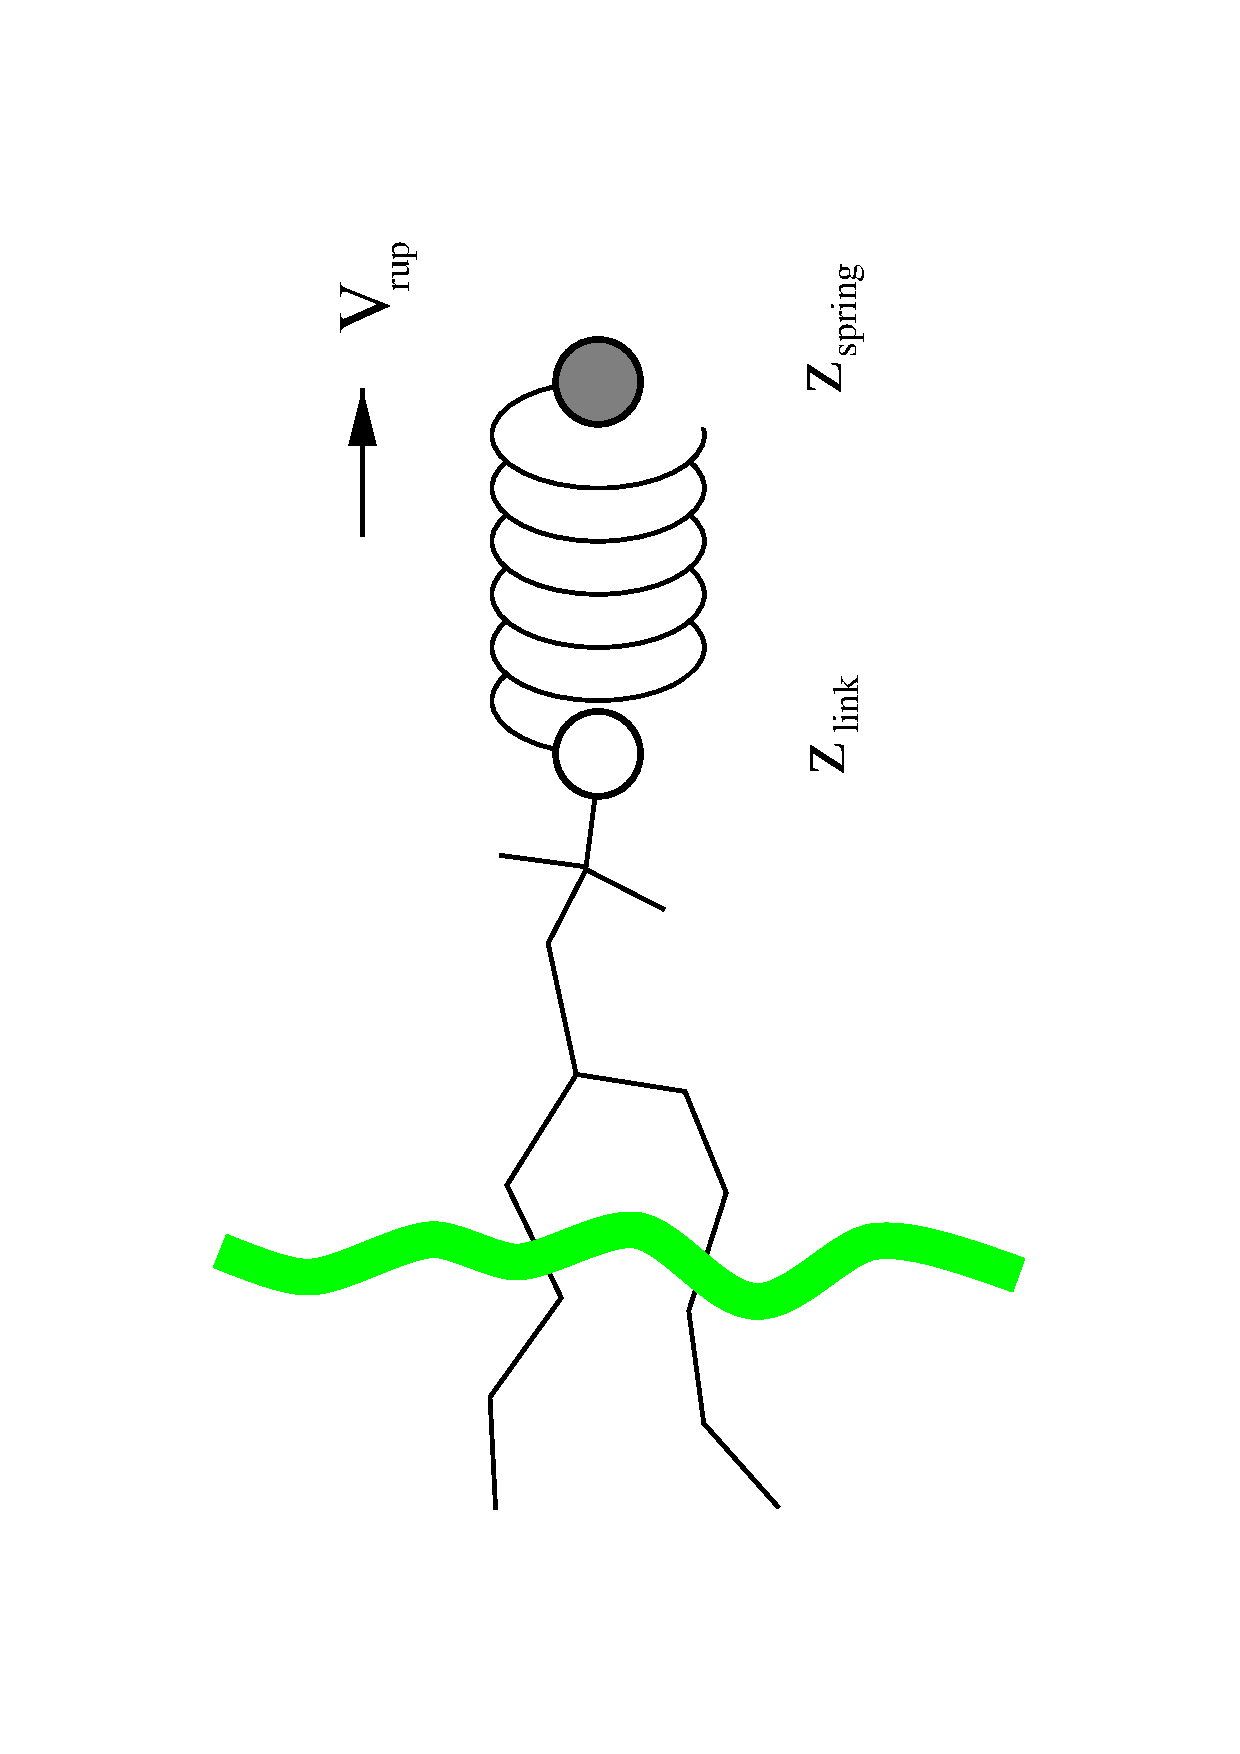
\includegraphics[width=6cm,angle=270]{plots/pull}}
\caption{Schematic picture of pulling a lipid out of a lipid bilayer
with umbrella pulling. $V_{rup}$ is the velocity at which the spring is
retracted, $Z_{link}$ is the atom to which the spring is attached and
$Z_{spring}$ is the location of the spring.}
\label{fig:pull} 
\end{figure}

Several different pull types, i.e. ways to apply the pull force, are supported,
and in all cases the reference distance can be constant
or linearly changing with time.
\begin{enumerate}
\item{\textbf{Umbrella pulling}\swapindexquiet{umbrella}{pulling}}
A harmonic potential is applied between
the centers of mass of two groups.
Thus, the force is proportional to the displacement.
\item{\textbf{Constraint pulling\swapindexquiet{constraint}{pulling}}}
The distance between the centers of mass of two groups is constrained.
The constraint force can be written to a file.
This method uses the SHAKE algorithm but only needs 1 iteration to be
exact if only two groups are constrained. 
\item{\textbf{Constant force pulling}}
A constant force is applied between the centers of mass of two groups.
Thus, the potential is linear.
In this case there is no reference distance of pull rate.
\item{\textbf{Flat bottom pulling}}
Like umbrella pulling, but the potential and force are zero for
coordinate values below ({\tt pull-coord?-type = flat-bottom}) or above
({\tt pull-coord?-type = flat-bottom-high}) a reference value.
This is useful for restraining e.g. the distance
between two molecules to a certain region.
\end{enumerate}
In addition, there are different types of reaction coordinates, so-called pull geometries.
These are set with the {\tt .mdp} option {\tt pull-coord?-geometry}.

\subsubsection{Definition of the center of mass}

In {\gromacs}, there are three ways to define the center of mass of a group.
The standard way is a ``plain'' center of mass, possibly with additional
weighting factors. With periodic boundary conditions it is no longer
possible to uniquely define the center of mass of a group of atoms.
Therefore, a reference atom is used. For determining the center of mass,
for all other atoms in the group, the closest periodic image to the reference
atom is used. This uniquely defines the center of mass.
By default, the middle (determined by the order in the topology) atom
is used as a reference atom, but the user can also select any other atom
if it would be closer to center of the group.

For a layered system, for instance a lipid bilayer, it may be of interest
to calculate the PMF of a lipid as function of its distance
from the whole bilayer. The whole bilayer can be taken as reference
group in that case, but it might also be of interest to define the
reaction coordinate for the PMF more locally. The {\tt .mdp} option
{\tt pull-coord?-geometry = cylinder} does not
use all the atoms of the reference group, but instead dynamically only those
within a cylinder with radius {\tt pull-cylinder-r} around the pull vector going
through the pull group. This only
works for distances defined in one dimension, and the cylinder is
oriented with its long axis along this one dimension. To avoid jumps in
the pull force, contributions of atoms are weighted as a function of distance
(in addition to the mass weighting):
\bea
w(r < r_\mathrm{cyl}) & = &
1-2 \left(\frac{r}{r_\mathrm{cyl}}\right)^2 + \left(\frac{r}{r_\mathrm{cyl}}\right)^4 \\
w(r \geq r_\mathrm{cyl}) & = & 0
\eea
Note that the radial dependence on the weight causes a radial force on
both cylinder group and the other pull group. This is an undesirable,
but unavoidable effect. To minimize this effect, the cylinder radius should
be chosen sufficiently large. The effective mass is 0.47 times that of
a cylinder with uniform weights and equal to the mass of uniform cylinder
of 0.79 times the radius.

\begin{figure}
\centerline{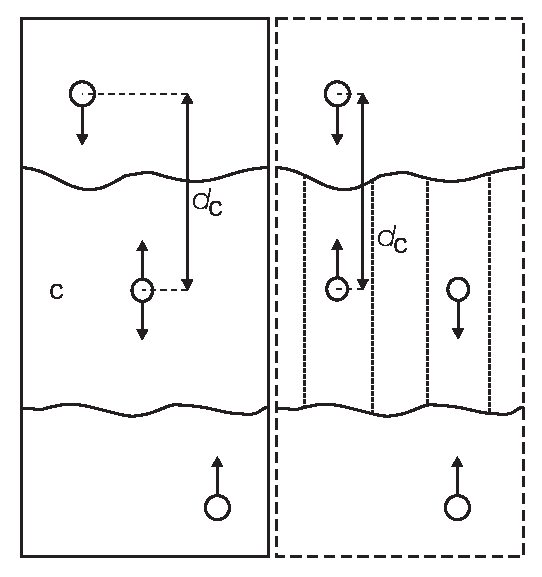
\includegraphics[width=6cm]{plots/pullref}}
\caption{Comparison of a plain center of mass reference group versus a cylinder
reference group applied to interface systems. C is the reference group.
The circles represent the center of mass of two groups plus the reference group,
$d_c$ is the reference distance.}
\label{fig:pullref} 
\end{figure}   

For a group of molecules in a periodic system, a plain reference group
might not be well-defined. An example is a water slab that is connected
periodically in $x$ and $y$, but has two liquid-vapor interfaces along $z$.
In such a setup, water molecules can evaporate from the liquid and they
will move through the vapor, through the periodic boundary, to the other
interface. Such a system is inherently periodic and there is no proper way
of defining a ``plain'' center of mass along $z$. A proper solution is to using
a cosine shaped weighting profile for all atoms in the reference group.
The profile is a cosine with a single period in the unit cell. Its phase
is optimized to give the maximum sum of weights, including mass weighting.
This provides a unique and continuous reference position that is nearly
identical to the plain center of mass position in case all atoms are all
within a half of the unit-cell length. See ref \cite{Engin2010a} for details.

When relative weights $w_i$ are used during the calculations, either
by supplying weights in the input or due to cylinder geometry
or due to cosine weighting,
the weights need to be scaled to conserve momentum:
\beq
w'_i = w_i
\left. \sum_{j=1}^N w_j \, m_j \right/ \sum_{j=1}^N w_j^2 \, m_j
\eeq
where $m_j$ is the mass of atom $j$ of the group.
The mass of the group, required for calculating the constraint force, is:
\beq
M = \sum_{i=1}^N w'_i \, m_i
\eeq
The definition of the weighted center of mass is:
\beq
\ve{r}_{com} = \left. \sum_{i=1}^N w'_i \, m_i \, \ve{r}_i \right/ M
\eeq
From the centers of mass the AFM, constraint, or umbrella force $\ve{F}_{\!com}$
on each group can be calculated.
The force on the center of mass of a group is redistributed to the atoms
as follows:
\beq
\ve{F}_{\!i} = \frac{w'_i \, m_i}{M} \, \ve{F}_{\!com}
\eeq

\subsubsection{Definition of the pull direction}

The most common setup is to pull along the direction of the vector containing
the two pull groups, this is selected with
{\tt pull-coord?-geometry = distance}. You might want to pull along a certain
vector instead, which is selected with {\tt pull-coord?-geometry = direction}.
But this can cause unwanted torque forces in the system, unless you pull against a reference group with (nearly) fixed orientation, e.g. a membrane protein embedded in a membrane along x/y while pulling along z. If your reference group does not have a fixed orientation, you should probably use
{\tt pull-coord?-geometry = direction-relative}, see \figref{pulldirrel}.
Since the potential now depends on the coordinates of two additional groups defining the orientation, the torque forces will work on these two groups.

\begin{figure}
\centerline{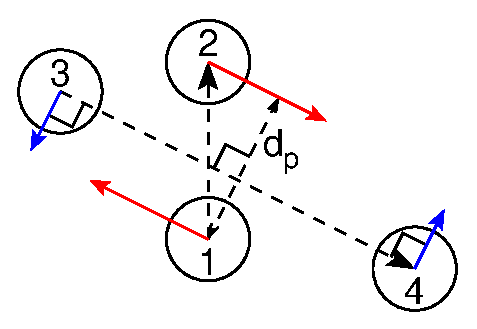
\includegraphics[width=5cm]{plots/pulldirrel}}
\caption{The pull setup for geometry {\tt direction-relative}. The ``normal'' pull groups are 1 and 2. Groups 3 and 4 define the pull direction and thus the direction of the normal pull forces (red). This leads to reaction forces (blue) on groups 3 and 4, which are perpendicular to the pull direction. Their magnitude is given by the ``normal'' pull force times the ratio of $d_p$ and the distance between groups 3 and 4.}
\label{fig:pulldirrel} 
\end{figure}   

\subsubsection{Definition of the angle and dihedral pull geometries}
Four pull groups are required for {\tt pull-coord?-geometry = angle}. In the same way as for geometries with two groups, each consecutive pair of groups
$i$ and $i+1$ define a vector connecting the COMs of groups $i$ and $i+1$. The angle is defined as the angle between the two resulting vectors.
E.g., the {\tt .mdp} option {\tt pull-coord?-groups = 1 2 2 4} defines the angle between the vector from the COM of group 1 to the COM of group 2
and the vector from the COM of group 2 to the COM of group 4.
The angle takes values in the closed interval [0, 180] deg.
For {\tt pull-coord?-geometry = angle-axis} the angle is defined with respect to a reference axis given by {\tt pull-coord?-vec} and only two groups need to be given.
The dihedral geometry requires six pull groups. These pair up in the same way as described above and so define three vectors. The dihedral angle is defined as the angle between the two
planes spanned by the two first and the two last vectors. Equivalently, the dihedral angle can be seen as the angle between the first and the third
vector when these vectors are projected onto a plane normal to the second vector (the axis vector).
As an example, consider a dihedral angle involving four groups: 1, 5, 8 and 9. Here, the {\tt .mdp} option
{\tt pull-coord?-groups = 8 1 1 5 5 9} specifies the three vectors that define the dihedral angle:
the first vector is the COM distance vector from group 8 to 1, the second vector is the COM distance vector from group 1 to 5, and the third vector is the COM distance vector from group 5 to 9.
The dihedral angle takes values in the interval (-180, 180] deg and has periodic boundaries.

\subsubsection{Limitations}
There is one theoretical limitation:
strictly speaking, constraint forces can only be calculated between
groups that are not connected by constraints to the rest of the system.
If a group contains part of a molecule of which the bond lengths
are constrained, the pull constraint and LINCS or SHAKE bond constraint
algorithms should be iterated simultaneously. This is not done in {\gromacs}.
This means that for simulations with {\tt constraints = all-bonds}
in the {\tt .mdp} file pulling is, strictly speaking,
limited to whole molecules or groups of molecules.
In some cases this limitation can be avoided by using the free energy code,
see \secref{fepmf}.
In practice, the errors caused by not iterating the two constraint
algorithms can be negligible when the pull group consists of a large
amount of atoms and/or the pull force is small.
In such cases, the constraint correction displacement of the pull group
is small compared to the bond lengths.



\section{\normindex{Enforced Rotation}}
\index{rotational pulling|see{enforced rotation}}
\index{pulling, rotational|see{enforced rotation}}
\label{sec:rotation}

\mathchardef\mhyphen="2D
\newcommand{\rotiso     }{^\mathrm{iso}}
\newcommand{\rotisopf   }{^\mathrm{iso\mhyphen pf}}
\newcommand{\rotpm      }{^\mathrm{pm}}
\newcommand{\rotpmpf    }{^\mathrm{pm\mhyphen pf}}
\newcommand{\rotrm      }{^\mathrm{rm}}
\newcommand{\rotrmpf    }{^\mathrm{rm\mhyphen pf}}
\newcommand{\rotrmtwo   }{^\mathrm{rm2}}
\newcommand{\rotrmtwopf }{^\mathrm{rm2\mhyphen pf}}
\newcommand{\rotflex    }{^\mathrm{flex}}
\newcommand{\rotflext   }{^\mathrm{flex\mhyphen t}}
\newcommand{\rotflextwo }{^\mathrm{flex2}}
\newcommand{\rotflextwot}{^\mathrm{flex2\mhyphen t}}

This module can be used to enforce the rotation of a group of atoms, as {\eg}
a protein subunit. There are a variety of rotation potentials, among them
complex ones that allow flexible adaptations of both the rotated subunit as
well as the local rotation axis during the simulation. An example application 
can be found in ref. \cite{Kutzner2011}.

\begin{figure}
\centerline{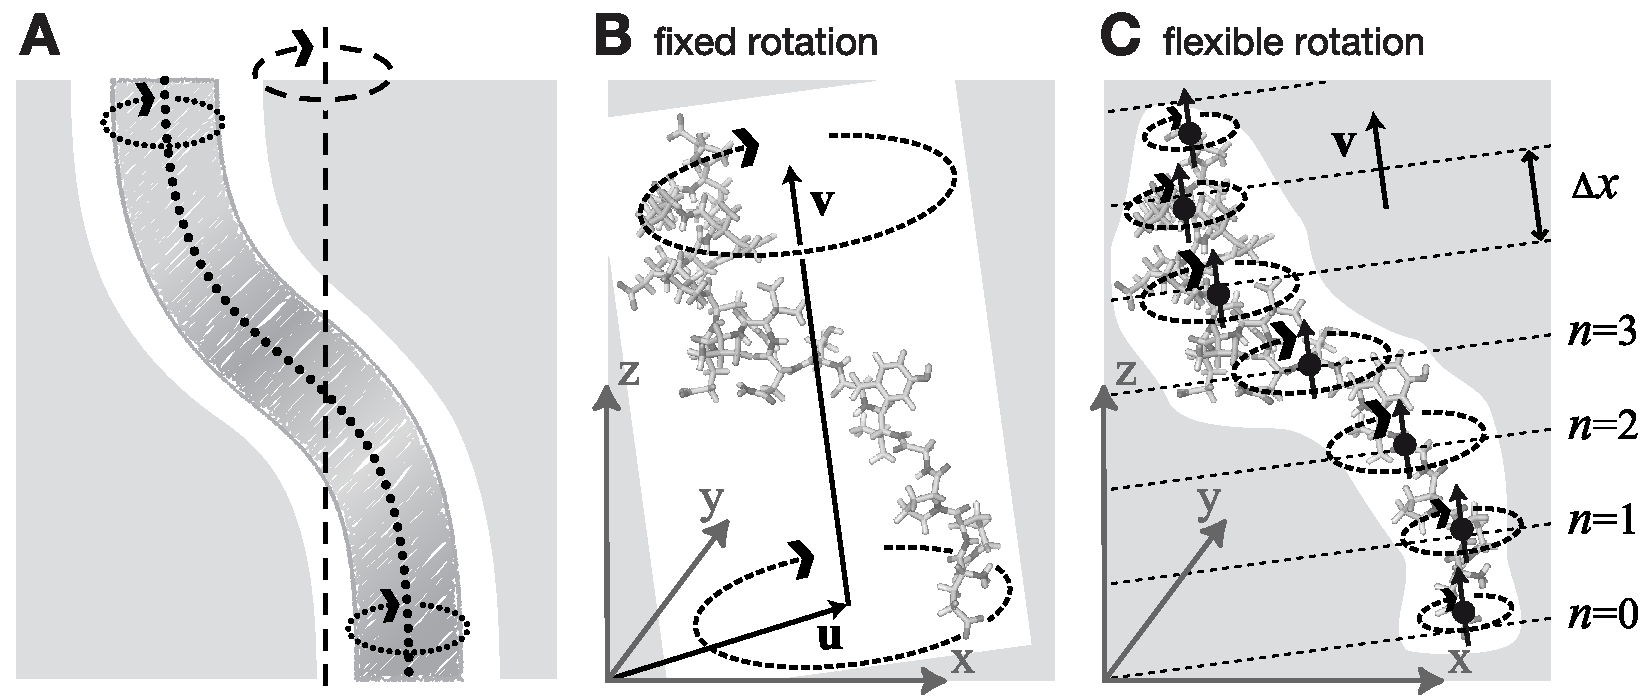
\includegraphics[width=13cm]{plots/rotation.pdf}}
\caption[Fixed and flexible axis rotation]{Comparison of fixed and flexible axis
rotation. 
{\sf A:} Rotating the sketched shape inside the white tubular cavity can create
artifacts when a fixed rotation axis (dashed) is used. More realistically, the
shape would revolve like a flexible pipe-cleaner (dotted) inside the bearing (gray). 
{\sf B:} Fixed rotation around an axis \ve{v} with a pivot point
specified by the vector \ve{u}. 
{\sf C:} Subdividing the rotating fragment into slabs with separate rotation
axes ($\uparrow$) and pivot points ($\bullet$) for each slab allows for
flexibility. The distance between two slabs with indices $n$ and $n+1$ is $\Delta x$.}
\label{fig:rotation}
\end{figure}

\begin{figure}
\centerline{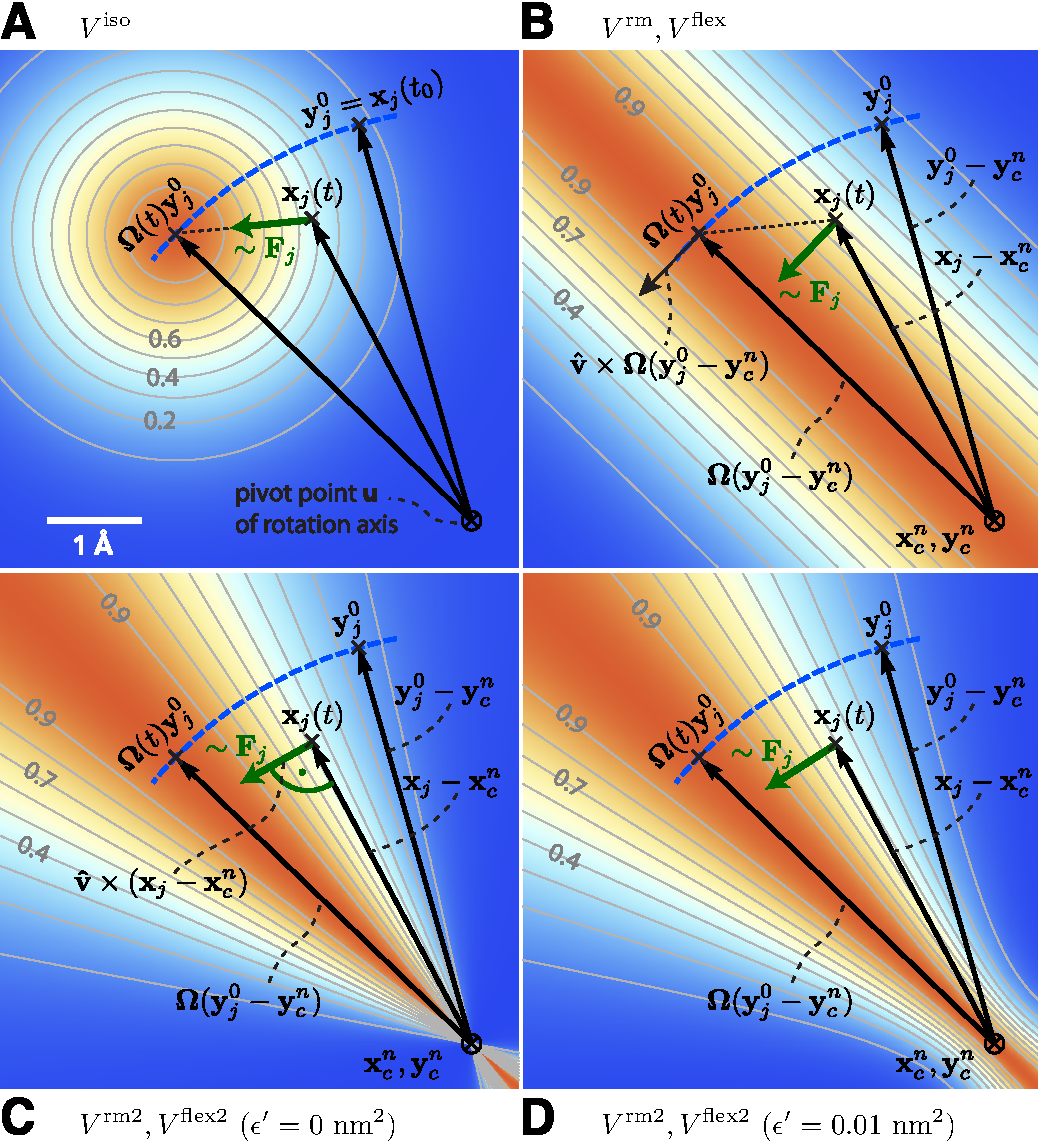
\includegraphics[width=13cm]{plots/equipotential.pdf}}
\caption{Selection of different rotation potentials and definition of notation.
All four potentials $V$ (color coded) are shown for a single atom at position
$\ve{x}_j(t)$.
{\sf A:} Isotropic potential $V\rotiso$,
{\sf B:} radial motion potential $V\rotrm$ and flexible potential
$V\rotflex$,
{\sf C--D:} radial motion\,2 potential $V\rotrmtwo$ and
flexible\,2 potential $V\rotflextwo$ for $\epsilon' = 0$\,nm$^2$ {\sf (C)}
and $\epsilon' = 0.01$\,nm$^2$ {\sf (D)}. The rotation axis is perpendicular to
the plane and marked by $\otimes$. The light gray contours indicate Boltzmann factors
$e^{-V/(k_B T)}$ in the $\ve{x}_j$-plane for $T=300$\,K and
$k=200$\,kJ/(mol$\cdot$nm$^2$). The green arrow shows the direction of the
force $\ve{F}_{\!j}$ acting on atom $j$; the blue dashed line indicates the
motion of the reference position.}
\label{fig:equipotential}
\end{figure}

\subsection{Fixed Axis Rotation}
\subsubsection{Stationary Axis with an Isotropic Potential}
In the fixed axis approach (see \figref{rotation}B), torque on a group of $N$
atoms with positions $\ve{x}_i$ (denoted ``rotation group'') is applied by
rotating a reference set of atomic positions -- usually their initial positions
$\ve{y}_i^0$ -- at a constant angular velocity $\omega$ around an axis
defined by a direction vector $\hat{\ve{v}}$ and a pivot point \ve{u}.
To that aim, each atom with position $\ve{x}_i$ is attracted by a
``virtual spring'' potential to its moving reference position
$\ve{y}_i = \mathbf{\Omega}(t) (\ve{y}_i^0 - \ve{u})$,
where $\mathbf{\Omega}(t)$ is a matrix that describes the rotation around the
axis. In the simplest case, the ``springs'' are described by a harmonic
potential,
\beq
V\rotiso = \frac{k}{2} \sum_{i=1}^{N} w_i \left[ \mathbf{\Omega}(t)
(\ve{y}_i^0 - \ve{u}) - (\ve{x}_i - \ve{u})  \right]^2 ,
\label{eqn:potiso}
\eeq
with optional mass-weighted prefactors $w_i = N \, m_i/M$ with total mass
$M = \sum_{i=1}^N m_i$.
The rotation matrix $\mathbf{\Omega}(t)$ is 
\newcommand{\omcost}{\,\xi\,}   % abbreviation
\begin{displaymath}
\mathbf{\Omega}(t) =  
\left(   
\begin{array}{ccc}
\cos\omega t + v_x^2\omcost       & v_x v_y\omcost - v_z\sin\omega t  & v_x v_z\omcost + v_y\sin\omega t\\
v_x v_y\omcost + v_z\sin\omega t  & \cos\omega t + v_y^2\omcost       & v_y v_z\omcost - v_x\sin\omega t\\
v_x v_z\omcost - v_y\sin\omega t  & v_y v_z\omcost + v_x\sin\omega t  & \cos\omega t + v_z^2\omcost     \\
\end{array}
\right) ,
\end{displaymath}
where $v_x$, $v_y$, and $v_z$ are the components of the normalized rotation vector
$\hat{\ve{v}}$, and $\omcost := 1-\cos(\omega t)$. As illustrated in
\figref{equipotential}A for a single atom $j$, the
rotation matrix $\mathbf{\Omega}(t)$ operates on the initial reference positions
$\ve{y}_j^0 = \ve{x}_j(t_0)$ of atom $j$ at $t=t_0$. At a later
time $t$, the reference position has rotated away from its initial place
(along the blue dashed line), resulting in the force
\beq
\ve{F}_{\!j}\rotiso 
= -\nabla_{\!j} \, V\rotiso 
= k \, w_j \left[
\mathbf{\Omega}(t) (\ve{y}_j^0 - \ve{u}) - (\ve{x}_j - \ve{u} ) \right] ,
\label{eqn:force_fixed}
\eeq
which is directed towards the reference position.


\subsubsection{Pivot-Free Isotropic Potential}
Instead of a fixed pivot vector \ve{u} this potential uses the center of
mass $\ve{x}_c$ of the rotation group as pivot for the rotation axis,
\beq
\ve{x}_c   = \frac{1}{M} \sum_{i=1}^N m_i \ve{x}_i 
\label{eqn:com}
\mbox{\hspace{4ex}and\hspace{4ex}}
\ve{y}_c^0 = \frac{1}{M} \sum_{i=1}^N m_i \ve{y}_i^0 \ ,
\eeq
which yields the ``pivot-free'' isotropic potential
\beq
V\rotisopf = \frac{k}{2} \sum_{i=1}^{N} w_i \left[ \mathbf{\Omega}(t)
(\ve{y}_i^0 - \ve{y}_c^0) - (\ve{x}_i - \ve{x}_c) \right]^2 ,
\label{eqn:potisopf}
\eeq
with forces
\beq
\mathbf{F}_{\!j}\rotisopf = k \, w_j 
\left[ 
\mathbf{\Omega}(t) ( \ve{y}_j^0 - \ve{y}_c^0) 
                 - ( \ve{x}_j   - \ve{x}_c )
\right] .
\label{eqn:force_isopf}
\eeq
Without mass-weighting, the pivot $\ve{x}_c$ is the geometrical center of
the group. 
\label{sec:fixed}

\subsubsection{Parallel Motion Potential Variant}
The forces generated by the isotropic potentials
(\eqnsref{potiso}{potisopf}) also contain components parallel
to the rotation axis and thereby restrain motions along the axis of either the
whole rotation group (in case of $V\rotiso$) or within
the rotation group (in case of $V\rotisopf$). For cases where
unrestrained motion along the axis is preferred, we have implemented a 
``parallel motion'' variant by eliminating all components parallel to the
rotation axis for the potential. This is achieved by projecting the distance
vectors between reference and actual positions
\beq
\ve{r}_i = \mathbf{\Omega}(t) (\ve{y}_i^0 - \ve{u}) - (\ve{x}_i - \ve{u})
\eeq
onto the plane perpendicular to the rotation vector,
\beq
\label{eqn:project}
\ve{r}_i^\perp :=  \ve{r}_i - (\ve{r}_i \cdot \hat{\ve{v}})\hat{\ve{v}} \ ,
\eeq
yielding
\bea
\nonumber
V\rotpm &=& \frac{k}{2} \sum_{i=1}^{N} w_i ( \ve{r}_i^\perp )^2 \\
        &=& \frac{k}{2} \sum_{i=1}^{N} w_i
 \left\lbrace
 \mathbf{\Omega}(t)
   (\ve{y}_i^0 - \ve{u}) - (\ve{x}_i - \ve{u})  \right. \nonumber \\
&& \left. - \left\lbrace
\left[ \mathbf{\Omega}(t)(\ve{y}_i^0 - \ve{u}) - (\ve{x}_i - \ve{u}) \right] \cdot\hat{\ve{v}}
  \right\rbrace\hat{\ve{v}} \right\rbrace^2 ,
\label{eqn:potpm}
\eea
and similarly
\beq
\ve{F}_{\!j}\rotpm = k \, w_j \, \ve{r}_j^\perp .
\label{eqn:force_pm}
\eeq

\subsubsection{Pivot-Free Parallel Motion Potential}
Replacing in \eqnref{potpm} the fixed pivot \ve{u} by the center 
of mass $\ve{x_c}$ yields the pivot-free variant of the parallel motion
potential. With
\beq
\ve{s}_i = \mathbf{\Omega}(t) (\ve{y}_i^0 - \ve{y}_c^0) - (\ve{x}_i - \ve{x}_c)
\eeq
the respective potential and forces are
\bea
V\rotpmpf &=& \frac{k}{2} \sum_{i=1}^{N} w_i ( \ve{s}_i^\perp )^2 \ , \\
\label{eqn:potpmpf}
\ve{F}_{\!j}\rotpmpf &=& k \, w_j \, \ve{s}_j^\perp .
\label{eqn:force_pmpf}
\eea

\subsubsection{Radial Motion Potential}
In the above variants, the minimum of the rotation potential is either a single
point at the reference position $\ve{y}_i$ (for the isotropic potentials) or a
single line through $\ve{y}_i$ parallel to the rotation axis (for the
parallel motion potentials). As a result, radial forces restrict radial motions
of the atoms. The two subsequent types of rotation potentials, $V\rotrm$
and $V\rotrmtwo$, drastically reduce or even eliminate this effect. The first
variant, $V\rotrm$ (\figref{equipotential}B), eliminates all force
components parallel to the vector connecting the reference atom and the
rotation axis,
\beq
V\rotrm = \frac{k}{2} \sum_{i=1}^{N} w_i \left[
\ve{p}_i
\cdot(\ve{x}_i - \ve{u}) \right]^2 ,
\label{eqn:potrm}
\eeq
with
\beq
\ve{p}_i := 
\frac{\hat{\ve{v}}\times \mathbf{\Omega}(t) (\ve{y}_i^0 - \ve{u})} {\| \hat{\ve{v}}\times \mathbf{\Omega}(t) (\ve{y}_i^0 - \ve{u})\|} \ .
\eeq
This variant depends only on the distance $\ve{p}_i \cdot (\ve{x}_i -
\ve{u})$ of atom $i$ from the plane spanned by $\hat{\ve{v}}$ and
$\mathbf{\Omega}(t)(\ve{y}_i^0 - \ve{u})$. The resulting force is
\beq
\mathbf{F}_{\!j}\rotrm =
 -k \, w_j \left[ \ve{p}_j\cdot(\ve{x}_j - \ve{u}) \right] \,\ve{p}_j \,  .
\label{eqn:potrm_force}
\eeq

\subsubsection{Pivot-Free Radial Motion Potential}
Proceeding similar to the pivot-free isotropic potential yields a pivot-free
version of the above potential. With
\beq
\ve{q}_i := 
\frac{\hat{\ve{v}}\times \mathbf{\Omega}(t) (\ve{y}_i^0 - \ve{y}_c^0)} {\| \hat{\ve{v}}\times \mathbf{\Omega}(t) (\ve{y}_i^0 - \ve{y}_c^0)\|} \, ,
\eeq
the potential and force for the pivot-free variant of the radial motion potential read
\bea
V\rotrmpf & = & \frac{k}{2} \sum_{i=1}^{N} w_i \left[
\ve{q}_i
\cdot(\ve{x}_i - \ve{x}_c)
\right]^2 \, , \\
\label{eqn:potrmpf}
\mathbf{F}_{\!j}\rotrmpf & = &
 -k \, w_j \left[ \ve{q}_j\cdot(\ve{x}_j - \ve{x}_c) \right] \,\ve{q}_j 
 + k   \frac{m_j}{M} \sum_{i=1}^{N} w_i \left[
 \ve{q}_i\cdot(\ve{x}_i - \ve{x}_c) \right]\,\ve{q}_i \, .
\label{eqn:potrmpf_force}
\eea

\subsubsection{Radial Motion 2 Alternative Potential}
As seen in \figref{equipotential}B, the force resulting from
$V\rotrm$ still contains a small, second-order radial component. In most
cases, this perturbation is tolerable; if not, the following
alternative, $V\rotrmtwo$, fully eliminates the radial contribution to the
force, as depicted in \figref{equipotential}C,
\beq
V\rotrmtwo = 
\frac{k}{2} \sum_{i=1}^{N} w_i\, 
\frac{\left[ (\hat{\ve{v}} \times ( \ve{x}_i - \ve{u} ))
\cdot \mathbf{\Omega}(t)(\ve{y}_i^0 - \ve{u}) \right]^2}
{\| \hat{\ve{v}} \times (\ve{x}_i - \ve{u}) \|^2 +
\epsilon'} \, ,
\label{eqn:potrm2}
\eeq
where a small parameter $\epsilon'$ has been introduced to avoid singularities.
For $\epsilon'=0$\,nm$^2$, the equipotential planes are spanned by $\ve{x}_i -
\ve{u}$ and $\hat{\ve{v}}$, yielding a force 
perpendicular to $\ve{x}_i - \ve{u}$, thus not contracting or
expanding structural parts that moved away from or toward the rotation axis.

Choosing a small positive  $\epsilon'$ ({\eg},
$\epsilon'=0.01$\,nm$^2$, \figref{equipotential}D) in the denominator of
\eqnref{potrm2} yields a well-defined potential and continuous forces also 
close to the rotation axis, which is not the case for $\epsilon'=0$\,nm$^2$ 
(\figref{equipotential}C). With
\bea
\ve{r}_i & := & \mathbf{\Omega}(t)(\ve{y}_i^0 - \ve{u})\\
\ve{s}_i & := & \frac{\hat{\ve{v}} \times (\ve{x}_i -
\ve{u} ) }{ \| \hat{\ve{v}} \times (\ve{x}_i - \ve{u})
\| } \equiv \; \Psi_{i} \;\; {\hat{\ve{v}} \times
(\ve{x}_i-\ve{u} ) }\\
\Psi_i^{*}   & := & \frac{1}{ \| \hat{\ve{v}} \times
(\ve{x}_i-\ve{u}) \|^2 + \epsilon'}
\eea
the force on atom $j$ reads
\beq
\ve{F}_{\!j}\rotrmtwo  = 
- k\; 
\left\lbrace w_j\;
(\ve{s}_j\cdot\ve{r}_{\!j})\;
\left[ \frac{\Psi_{\!j}^*   }{\Psi_{\!j}  }  \ve{r}_{\!j} 
     - \frac{\Psi_{\!j}^{*2}}{\Psi_{\!j}^3}
     (\ve{s}_j\cdot\ve{r}_{\!j})\ve{s}_j \right]
\right\rbrace \times \hat{\ve{v}} .
\label{eqn:potrm2_force}
\eeq

\subsubsection{Pivot-Free Radial Motion 2 Potential}
The pivot-free variant of the above potential is
\beq
V\rotrmtwopf = 
\frac{k}{2} \sum_{i=1}^{N} w_i\, 
\frac{\left[ (\hat{\ve{v}} \times ( \ve{x}_i - \ve{x}_c ))
\cdot \mathbf{\Omega}(t)(\ve{y}_i^0 - \ve{y}_c) \right]^2}
{\| \hat{\ve{v}} \times (\ve{x}_i - \ve{x}_c) \|^2 +
\epsilon'} \, .
\label{eqn:potrm2pf}
\eeq
With
\bea
\ve{r}_i & := & \mathbf{\Omega}(t)(\ve{y}_i^0 - \ve{y}_c)\\
\ve{s}_i & := & \frac{\hat{\ve{v}} \times (\ve{x}_i -
\ve{x}_c ) }{ \| \hat{\ve{v}} \times (\ve{x}_i - \ve{x}_c)
\| } \equiv \; \Psi_{i} \;\; {\hat{\ve{v}} \times
(\ve{x}_i-\ve{x}_c ) }\\ \Psi_i^{*}   & := & \frac{1}{ \| \hat{\ve{v}} \times
(\ve{x}_i-\ve{x}_c) \|^2 + \epsilon'}
\eea
the force on atom $j$ reads
\bea
\nonumber
\ve{F}_{\!j}\rotrmtwopf & = &
- k\; 
\left\lbrace w_j\;
(\ve{s}_j\cdot\ve{r}_{\!j})\;
\left[ \frac{\Psi_{\!j}^*   }{\Psi_{\!j}  } \ve{r}_{\!j} 
     - \frac{\Psi_{\!j}^{*2}}{\Psi_{\!j}^3}
     (\ve{s}_j\cdot\ve{r}_{\!j})\ve{s}_j \right]
\right\rbrace \times \hat{\ve{v}}\\
     & &
+ k\;\frac{m_j}{M} \left\lbrace \sum_{i=1}^{N}
w_i\;(\ve{s}_i\cdot\ve{r}_i) \; 
\left[ \frac{\Psi_i^*   }{\Psi_i  }  \ve{r}_i
     - \frac{\Psi_i^{*2}}{\Psi_i^3} (\ve{s}_i\cdot\ve{r}_i )\;
     \ve{s}_i \right] \right\rbrace \times \hat{\ve{v}} \, .
\label{eqn:potrm2pf_force}
\eea

\subsection{Flexible Axis Rotation}
As sketched in \figref{rotation}A--B, the rigid body behavior of
the fixed axis rotation scheme is a drawback for many applications. In
particular, deformations of the rotation group are suppressed when the
equilibrium atom positions directly depend on the reference positions. 
To avoid this limitation, \eqnsref{potrmpf}{potrm2pf}
will now be generalized towards a ``flexible axis'' as sketched in
\figref{rotation}C. This will be achieved by subdividing the
rotation group into a set of equidistant slabs perpendicular to
the rotation vector, and by applying a separate rotation potential to each
of these slabs. \figref{rotation}C shows the midplanes of the slabs 
as dotted straight lines and the centers as thick black dots.

To avoid discontinuities in the potential and in the forces, we define
``soft slabs'' by weighing the contributions of each
slab $n$ to the total potential function $V\rotflex$ by a Gaussian
function
\beq
\label{eqn:gaussian}
g_n(\ve{x}_i) = \Gamma \ \mbox{exp} \left(
-\frac{\beta_n^2(\ve{x}_i)}{2\sigma^2}  \right) ,
\eeq
centered at the midplane of the $n$th slab. Here $\sigma$ is the width
of the Gaussian function, $\Delta x$ the distance between adjacent slabs, and
\beq
\beta_n(\ve{x}_i) := \ve{x}_i \cdot \hat{\ve{v}} - n \, \Delta x \, .
\eeq
%
\begin{figure}
\centerline{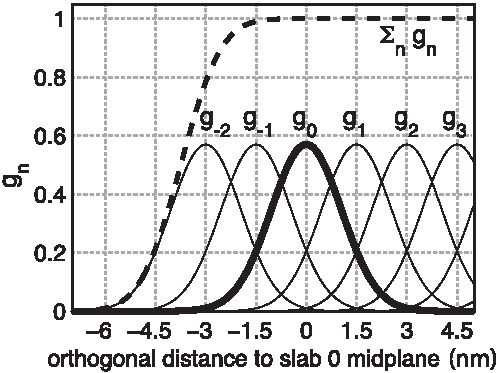
\includegraphics[width=6.5cm]{plots/gaussians.pdf}}
\caption{Gaussian functions $g_n$ centered at $n \, \Delta x$ for a slab
distance $\Delta x = 1.5$ nm and $n \geq -2$. Gaussian function $g_0$ is
highlighted in bold; the dashed line depicts the sum of the shown Gaussian
functions.}
\label{fig:gaussians}
\end{figure}
%
A most convenient choice is $\sigma = 0.7 \Delta x$ and
\begin{displaymath}
1/\Gamma = \sum_{n \in Z}
\mbox{exp}
\left(-\frac{(n - \frac{1}{4})^2}{2\cdot 0.7^2}\right)
\approx 1.75464 \, ,
\end{displaymath}
which yields a nearly constant sum, essentially independent of $\ve{x}_i$
(dashed line in \figref{gaussians}), {\ie},
\beq
\sum_{n \in Z} g_n(\ve{x}_i) =  1 + \epsilon(\ve{x}_i) \, ,
\label{eqn:normal}
\eeq
with $ | \epsilon(\ve{x}_i) | < 1.3\cdot 10^{-4}$. This choice also
implies that the individual contributions to the force from the slabs add up to
unity such that no further normalization is required.

To each slab center $\ve{x}_c^n$, all atoms contribute by their
Gaussian-weighted (optionally also mass-weighted) position vectors 
$g_n(\ve{x}_i) \, \ve{x}_i$. The
instantaneous slab centers $\ve{x}_c^n$ are calculated from the
current positions $\ve{x}_i$,
\beq
\label{eqn:defx0} 
\ve{x}_c^n =
\frac{\sum_{i=1}^N g_n(\ve{x}_i) \, m_i \, \ve{x}_i}
     {\sum_{i=1}^N g_n(\ve{x}_i) \, m_i} \, ,\\
\eeq
while the reference centers $\ve{y}_c^n$ are calculated from the reference 
positions $\ve{y}_i^0$,
\beq
\label{eqn:defy0}
\ve{y}_c^n =
\frac{\sum_{i=1}^N g_n(\ve{y}_i^0) \, m_i \, \ve{y}_i^0}
     {\sum_{i=1}^N g_n(\ve{y}_i^0) \, m_i} \, .
\eeq
Due to the rapid decay of $g_n$, each slab
will essentially involve contributions from atoms located within $\approx
3\Delta x$ from the slab center only.

\subsubsection{Flexible Axis Potential}
We consider two flexible axis variants. For the first variant,
the slab segmentation procedure with Gaussian weighting is applied to the radial 
motion potential (\eqnref{potrmpf}\,/\,\figref{equipotential}B),
yielding as the contribution of slab $n$
\begin{displaymath}
V^n = 
\frac{k}{2} \sum_{i=1}^{N} w_i \, g_n(\ve{x}_i) 
\left[
\ve{q}_i^n
\cdot
 (\ve{x}_i - \ve{x}_c^n) 
\right]^2  ,
\label{eqn:flexpot}
\end{displaymath}
and a total potential function
\beq 
V\rotflex = \sum_n V^n \, .
\label{eqn:potflex}
\eeq
Note that the global center of mass $\ve{x}_c$ used in
\eqnref{potrmpf} is now replaced by $\ve{x}_c^n$, the center of mass of
the slab. With
\bea
\ve{q}_i^n & := & \frac{\hat{\ve{v}} \times
\mathbf{\Omega}(t)(\ve{y}_i^0 - \ve{y}_c^n) }{ \| \hat{\ve{v}}
\times \mathbf{\Omega}(t)(\ve{y}_i^0 - \ve{y}_c^n) \| } \\
b_i^n         & := & \ve{q}_i^n \cdot (\ve{x}_i - \ve{x}_c^n) \, ,
\eea
the resulting force on atom $j$ reads
\bea
\nonumber\hspace{-15mm}
\ve{F}_{\!j}\rotflex &=&
- \, k \, w_j \sum_n g_n(\ve{x}_j) \, b_j^n \left\lbrace  \ve{q}_j^n -
b_j^n \frac{\beta_n(\ve{x}_j)}{2\sigma^2} \hat{\ve{v}} \right\rbrace \\ & &
+ \, k \, m_j \sum_n \frac{g_n(\ve{x}_j)}{\sum_h g_n(\ve{x}_h)}
\sum_{i=1}^{N} w_i \, g_n(\ve{x}_i) \, b_i^n \left\lbrace 
\ve{q}_i^n -\frac{\beta_n(\ve{x}_j)}{\sigma^2}
\left[ \ve{q}_i^n \cdot (\ve{x}_j - \ve{x}_c^n )\right]
\hat{\ve{v}} \right\rbrace .
\label{eqn:potflex_force}
\eea
%
Note that for $V\rotflex$, as defined, the slabs are fixed in space and so
are the reference centers $\ve{y}_c^n$. If during the simulation the
rotation group moves too far in $\ve{v}$ direction, it may enter a
region where -- due to the lack of nearby reference positions -- no reference
slab centers are defined, rendering the potential evaluation impossible. 
We therefore have included a slightly modified version of this potential that
avoids this problem by attaching the midplane of slab $n=0$ to the center of mass 
of the rotation group, yielding slabs that move with the rotation group. 
This is achieved by subtracting the center of mass $\ve{x}_c$ of the
group from the positions, 
\beq
\tilde{\ve{x}}_i = \ve{x}_i - \ve{x}_c \, , \mbox{\ \ \ and \ \ } 
\tilde{\ve{y}}_i^0 = \ve{y}_i^0 - \ve{y}_c^0 \, ,
\label{eqn:trafo} 
\eeq
such that
\bea
V\rotflext 
  & = & \frac{k}{2} \sum_n \sum_{i=1}^{N} w_i \, g_n(\tilde{\ve{x}}_i)
  \left[ \frac{\hat{\ve{v}} \times \mathbf{\Omega}(t)(\tilde{\ve{y}}_i^0
  - \tilde{\ve{y}}_c^n) }{ \| \hat{\ve{v}} \times
\mathbf{\Omega}(t)(\tilde{\ve{y}}_i^0 -
\tilde{\ve{y}}_c^n) \| }
\cdot
 (\tilde{\ve{x}}_i - \tilde{\ve{x}}_c^n) 
\right]^2 .
\label{eqn:potflext}
\eea
To simplify the force derivation, and for efficiency reasons, we here assume
$\ve{x}_c$ to be constant, and thus $\partial \ve{x}_c / \partial x =
\partial \ve{x}_c / \partial y = \partial \ve{x}_c / \partial z = 0$. The
resulting force error is small (of order $O(1/N)$ or $O(m_j/M)$ if
mass-weighting is applied) and can therefore be tolerated. With this assumption,
the forces $\ve{F}\rotflext$ have the same form as
\eqnref{potflex_force}.

\subsubsection{Flexible Axis 2 Alternative Potential}
In this second variant, slab segmentation is applied to $V\rotrmtwo$
(\eqnref{potrm2pf}), resulting in a flexible axis potential without radial
force contributions (\figref{equipotential}C),
\beq
V\rotflextwo = 
\frac{k}{2} \sum_{i=1}^{N} \sum_n w_i\,g_n(\ve{x}_i) 
\frac{\left[ (\hat{\ve{v}} \times ( \ve{x}_i - \ve{x}_c^n ))
\cdot \mathbf{\Omega}(t)(\ve{y}_i^0 - \ve{y}_c^n) \right]^2}
{\| \hat{\ve{v}} \times (\ve{x}_i - \ve{x}_c^n) \|^2 +
\epsilon'} \, .
\label{eqn:potflex2}
\eeq
With
\bea
\ve{r}_i^n & := & \mathbf{\Omega}(t)(\ve{y}_i^0 - \ve{y}_c^n)\\
\ve{s}_i^n & := & \frac{\hat{\ve{v}} \times (\ve{x}_i -
\ve{x}_c^n ) }{ \| \hat{\ve{v}} \times (\ve{x}_i - \ve{x}_c^n)
\| } \equiv \; \psi_{i} \;\; {\hat{\ve{v}} \times (\ve{x}_i-\ve{x}_c^n ) }\\
\psi_i^{*}     & := & \frac{1}{ \| \hat{\ve{v}} \times (\ve{x}_i-\ve{x}_c^n) \|^2 + \epsilon'}\\ 
W_j^n          & := & \frac{g_n(\ve{x}_j)\,m_j}{\sum_h g_n(\ve{x}_h)\,m_h}\\
\ve{S}^n   & := & 
\sum_{i=1}^{N} w_i\;g_n(\ve{x}_i)
\; (\ve{s}_i^n\cdot\ve{r}_i^n)
\left[ \frac{\psi_i^*   }{\psi_i  }  \ve{r}_i^n
     - \frac{\psi_i^{*2}}{\psi_i^3} (\ve{s}_i^n\cdot\ve{r}_i^n )\;
     \ve{s}_i^n \right] \label{eqn:Sn}
\eea
the force on atom $j$ reads
\bea
\nonumber
\ve{F}_{\!j}\rotflextwo & = &
- k\; 
\left\lbrace \sum_n w_j\;g_n(\ve{x}_j)\;
(\ve{s}_j^n\cdot\ve{r}_{\!j}^n)\;
\left[ \frac{\psi_j^*   }{\psi_j  }  \ve{r}_{\!j}^n 
     - \frac{\psi_j^{*2}}{\psi_j^3} (\ve{s}_j^n\cdot\ve{r}_{\!j}^n)\;
     \ve{s}_{\!j}^n \right] \right\rbrace \times \hat{\ve{v}} \\
\nonumber
& &
+ k \left\lbrace \sum_n W_{\!j}^n \, \ve{S}^n \right\rbrace \times
\hat{\ve{v}}
- k \left\lbrace \sum_n W_{\!j}^n \; \frac{\beta_n(\ve{x}_j)}{\sigma^2} \frac{1}{\psi_j}\;\; 
\ve{s}_j^n \cdot 
\ve{S}^n \right\rbrace \hat{\ve{v}}\\ 
& & 
+ \frac{k}{2} \left\lbrace \sum_n w_j\;g_n(\ve{x}_j)
\frac{\beta_n(\ve{x}_j)}{\sigma^2} 
\frac{\psi_j^*}{\psi_j^2}( \ve{s}_j^n \cdot \ve{r}_{\!j}^n )^2 \right\rbrace
\hat{\ve{v}} .
\label{eqn:potflex2_force}
\eea

Applying transformation (\ref{eqn:trafo}) yields a ``translation-tolerant''
version of the flexible\,2 potential, $V\rotflextwot$. Again,
assuming that $\partial \ve{x}_c / \partial x$,  $\partial \ve{x}_c /
\partial y$, $\partial \ve{x}_c / \partial z$ are small, the
resulting equations for $V\rotflextwot$ and $\ve{F}\rotflextwot$ are
similar to those of $V\rotflextwo$ and $\ve{F}\rotflextwo$.

\subsection{Usage}
To apply enforced rotation, the particles $i$ that are to
be subjected to one of the rotation potentials are defined via index groups
{\tt rot-group0}, {\tt rot-group1}, etc., in the {\tt .mdp} input file. 
The reference positions $\ve{y}_i^0$ are
read from a special {\tt .trr} file provided to {\tt grompp}. If no such file is found,
$\ve{x}_i(t=0)$ are used as reference positions and written to {\tt .trr} such
that they can be used for subsequent setups. All parameters of the potentials
such as $k$, $\epsilon'$, etc. (\tabref{vars}) are provided as {\tt .mdp}
parameters; {\tt rot-type} selects the type of the potential. 
The option {\tt rot-massw} allows to choose whether or not to use
mass-weighted averaging. 
For the flexible potentials, a cutoff value $g_n^\mathrm{min}$ 
(typically  $g_n^\mathrm{min}=0.001$) makes shure that only
significant contributions to $V$ and \ve{F} are evaluated, {\ie} terms with 
$g_n(\ve{x}) < g_n^\mathrm{min}$ are omitted.
\tabref{quantities} summarizes observables that are written
to additional output files and which are described below.


\begin{table}[tbp]
\caption{Parameters used by the various rotation potentials.
{\sf x}'s indicate which parameter is actually used for a given potential.}
%\small

\newcommand{\kunit}{$\frac{\mathrm{kJ}}{\mathrm{mol} \cdot \mathrm{nm}^2}$}
\newcommand{\smtt}[1]{{\hspace{-0.5ex}\small #1\hspace{-0.5ex}}}
\label{tab:vars}
\begin{center}
\begin{tabular}{l>{$}l<{$}rccccccc}
\hline
parameter           &               &                      & $k$      & $\hat{\ve{v}}$ & $\ve{u}$     & $\omega$    & $\epsilon'$ & $\Delta x$        & $g_n^\mathrm{min}$ \\
\multicolumn{3}{l}{{\tt .mdp} input variable name}         & \smtt{k} & \smtt{vec}     & \smtt{pivot} & \smtt{rate} & \smtt{eps}  & \smtt{slab-dist}  & \smtt{min-gauss}   \\
unit                &               &                      & \kunit   & -              & nm           & $^\circ$/ps & nm$^2$      & nm                & \,-\,              \\[1mm]
\hline \multicolumn{2}{l}{fixed axis potentials:} & eqn.\\
isotropic           & V\rotiso      & (\ref{eqn:potiso})   & {\sf x}  & {\sf x}        & {\sf x}      & {\sf x}     & -           & -                 &  -                 \\
--- pivot-free      & V\rotisopf    & (\ref{eqn:potisopf}) & {\sf x}  & {\sf x}        & -            & {\sf x}     & -           & -                 &  -                 \\
parallel motion     & V\rotpm       & (\ref{eqn:potpm})    & {\sf x}  & {\sf x}        & {\sf x}      & {\sf x}     & -           & -                 &  -                 \\
--- pivot-free      & V\rotpmpf     & (\ref{eqn:potpmpf})  & {\sf x}  & {\sf x}        & -            & {\sf x}     & -           & -                 &  -                 \\
radial motion       & V\rotrm       & (\ref{eqn:potrm})    & {\sf x}  & {\sf x}        & {\sf x}      & {\sf x}     & -           & -                 &  -                 \\
--- pivot-free      & V\rotrmpf     & (\ref{eqn:potrmpf})  & {\sf x}  & {\sf x}        & -            & {\sf x}     & -           & -                 &  -                 \\
radial motion\,2    & V\rotrmtwo    & (\ref{eqn:potrm2})   & {\sf x}  & {\sf x}        & {\sf x}      & {\sf x}     & {\sf x}     & -                 &  -                 \\
--- pivot-free      & V\rotrmtwopf  & (\ref{eqn:potrm2pf}) & {\sf x}  & {\sf x}        & -            & {\sf x}     & {\sf x}     & -                 &  -                 \\ \hline
\multicolumn{2}{l}{flexible axis potentials:}  & eqn.\\
flexible            & V\rotflex     & (\ref{eqn:potflex})  & {\sf x}  & {\sf x}        & -            & {\sf x}     & -           & {\sf x}           &  {\sf x}           \\
--- transl. tol.    & V\rotflext    & (\ref{eqn:potflext}) & {\sf x}  & {\sf x}        & -            & {\sf x}     & -           & {\sf x}           &  {\sf x}           \\
flexible\,2         & V\rotflextwo  & (\ref{eqn:potflex2}) & {\sf x}  & {\sf x}        & -            & {\sf x}     & {\sf x}     & {\sf x}           &  {\sf x}           \\
--- transl. tol.    & V\rotflextwot &  -                   & {\sf x}  & {\sf x}        & -            & {\sf x}     & {\sf x}     & {\sf x}           &  {\sf x}           \\
\hline
\end{tabular}
\end{center}
\end{table}

\begin{table}
\caption{Quantities recorded in output files during enforced rotation simulations.
All slab-wise data is written every {\tt nstsout} steps, other rotation data every {\tt nstrout} steps.}
\label{tab:quantities}
\begin{center}
\begin{tabular}{llllcc}
\hline
quantity                                             & unit    & equation                          & output file     & fixed   & flexible\\ \hline
$V(t)$                                               & kJ/mol  & see \ref{tab:vars}                & {\tt rotation}  & {\sf x} & {\sf x} \\
$\theta_\mathrm{ref}(t)$                             & degrees & $\theta_\mathrm{ref}(t)=\omega t$ & {\tt rotation}  & {\sf x} & {\sf x} \\
$\theta_\mathrm{av}(t)$                              & degrees & (\ref{eqn:avangle})               & {\tt rotation}  & {\sf x} & -       \\
$\theta_\mathrm{fit}(t)$, $\theta_\mathrm{fit}(t,n)$ & degrees & (\ref{eqn:rmsdfit})               & {\tt rotangles} & -       & {\sf x} \\
$\ve{y}_0(n)$, $\ve{x}_0(t,n)$                       & nm      & (\ref{eqn:defx0}, \ref{eqn:defy0})& {\tt rotslabs}  & -       & {\sf x} \\
$\tau(t)$                                            & kJ/mol  & (\ref{eqn:torque})                & {\tt rotation}  & {\sf x} & -       \\
$\tau(t,n)$                                          & kJ/mol  & (\ref{eqn:torque})                & {\tt rottorque} & -       & {\sf x} \\ \hline
\end{tabular}
\end{center}
\end{table}


\subsubsection*{Angle of Rotation Groups: Fixed Axis}
For fixed axis rotation, the average angle $\theta_\mathrm{av}(t)$ of the 
group relative to the reference group is determined via the distance-weighted
angular deviation of all rotation group atoms from their reference positions,
\beq
\theta_\mathrm{av} = \left. \sum_{i=1}^{N} r_i \ \theta_i \right/ \sum_{i=1}^N r_i \ .
\label{eqn:avangle}
\eeq
Here, $r_i$ is the distance of the reference position to the rotation axis, and
the difference angles $\theta_i$ are determined from the atomic positions, 
projected onto a plane perpendicular to the rotation axis through pivot point
$\ve{u}$ (see \eqnref{project} for the definition of $\perp$),
\beq
\cos \theta_i = 
\frac{(\ve{y}_i-\ve{u})^\perp \cdot (\ve{x}_i-\ve{u})^\perp}
     { \| (\ve{y}_i-\ve{u})^\perp \cdot (\ve{x}_i-\ve{u})^\perp
     \| } \ .
\eeq
%
The sign of $\theta_\mathrm{av}$ is chosen such that
$\theta_\mathrm{av} > 0$ if the actual structure rotates ahead of the reference.

\subsubsection*{Angle of Rotation Groups: Flexible Axis}
For flexible axis rotation, two outputs are provided, the angle of the
entire rotation group, and separate angles for the segments in the slabs.
The angle of the entire rotation group is determined by an RMSD fit 
of $\ve{x}_i$
to the reference positions $\ve{y}_i^0$ at $t=0$, yielding $\theta_\mathrm{fit}$
as the angle by which the reference has to be rotated around $\hat{\ve{v}}$ 
for the optimal fit,
\beq
\mathrm{RMSD} \big( \ve{x}_i,\ \mathbf{\Omega}(\theta_\mathrm{fit})
\ve{y}_i^0 \big) \stackrel{!}{=} \mathrm{min} \, .
\label{eqn:rmsdfit}
\eeq
To determine the local angle for each slab $n$, both reference and actual
positions are weighted with the Gaussian function of slab $n$, and 
$\theta_\mathrm{fit}(t,n)$ is calculated as in \eqnref{rmsdfit}) from the
Gaussian-weighted positions.

For all angles, the {\tt .mdp} input option {\tt rot-fit-method} controls
whether a normal RMSD fit is performed or whether for the fit each
position $\ve{x}_i$ is put at the same distance to the rotation axis as its
reference counterpart $\ve{y}_i^0$. In the latter case, the RMSD
measures only angular differences, not radial ones.


\subsubsection*{Angle Determination by Searching the Energy Minimum}
Alternatively, for {\tt rot-fit-method = potential}, the angle of the rotation 
group is determined as the angle for which the rotation potential energy is minimal.
Therefore, the used rotation potential is additionally evaluated for a set of angles
around the current reference angle. In this case, the {\tt rotangles.log} output file
contains the values of the rotation potential at the chosen set of angles, while 
{\tt rotation.xvg} lists the angle with minimal potential energy.


\subsubsection*{Torque}
\label{torque}
The torque $\ve{\tau}(t)$ exerted by the rotation potential is calculated for fixed
axis rotation via
\beq
\ve{\tau}(t) = \sum_{i=1}^{N} \ve{r}_i(t) \times \ve{f}_{\!i}^\perp(t) ,
\label{eqn:torque}
\eeq
where $\ve{r}_i(t)$ is the distance vector from the rotation axis to
$\ve{x}_i(t)$ and $\ve{f}_{\!i}^\perp(t)$ is the force component
perpendicular to $\ve{r}_i(t)$ and $\hat{\ve{v}}$. For flexible axis
rotation, torques $\ve{\tau}_{\!n}$ are calculated for each slab using the
local rotation axis of the slab and the Gaussian-weighted positions.


\section{\normindex{Computational Electrophysiology}}
\label{sec:compel}

The Computational Electrophysiology (CompEL) protocol \cite{Kutzner2011b} allows the simulation of
ion flux through membrane channels, driven by transmembrane potentials or ion
concentration gradients. Just as in real cells, CompEL establishes transmembrane
potentials by sustaining a small imbalance of charges $\Delta q$ across the membrane,
which gives rise to a potential difference $\Delta U$ according to the membrane capacitance:
\beq
\Delta U = \Delta q / C_{membrane}
\eeq
The transmembrane electric field and concentration gradients are controlled by
{\tt .mdp} options, which allow the user to set reference counts for the ions on either side
of the membrane. If a difference between the actual and the reference numbers persists
over a certain time span, specified by the user, a number of ion/water pairs are
exchanged between the compartments until the reference numbers are restored.
Alongside the calculation of channel conductance and ion selectivity, CompEL simulations also
enable determination of the channel reversal potential, an important
characteristic obtained in electrophysiology experiments.

In a CompEL setup, the simulation system is divided into two compartments {\bf A} and {\bf B}
with independent ion concentrations. This is best achieved by using double bilayer systems with
a copy (or copies) of the channel/pore of interest in each bilayer (\figref{compelsetup} A, B).
If the channel axes point in the same direction, channel flux is observed
simultaneously at positive and negative potentials in this way, which is for instance
important for studying channel rectification.

\begin{figure}
\centerline{\includegraphics[width=13.5cm]{plots/compelsetup.pdf}}
\caption{Typical double-membrane setup for CompEL simulations (A, B).
Ion\,/\,water molecule exchanges will be performed as needed
between the two light blue volumes around the dotted black lines (A).
Plot (C) shows the potential difference $\Delta U$ resulting
from the selected charge imbalance $\Delta q_{ref}$ between the compartments.}
\label{fig:compelsetup}
\end{figure}

The potential difference $\Delta U$ across the membrane is easily calculated with the
{\tt gmx potential} utility. By this, the potential drop along $z$ or the
pore axis is exactly known in each time interval of the simulation (\figref{compelsetup} C).
Type and number of ions $n_i$ of charge $q_i$, traversing the channel in the simulation,
are written to the {\tt swapions.xvg} output file, from which the average channel
conductance $G$ in each interval $\Delta t$ is determined by:
\beq
G = \frac{\sum_{i} n_{i}q_{i}}{\Delta t \, \Delta U} \, .
\eeq
The ion selectivity is calculated as the number flux ratio of different species.
Best results are obtained by averaging these values over several overlapping time intervals.

The calculation of reversal potentials is best achieved using a small set of simulations in which a given
transmembrane concentration gradient is complemented with small ion imbalances of varying magnitude. For
example, if one compartment contains 1\,M salt and the other 0.1\,M, and given charge neutrality otherwise,
a set of simulations with $\Delta q = 0\,e$, $\Delta q = 2\,e$, $\Delta q = 4\,e$ could
be used. Fitting a straight line through the current-voltage relationship of all obtained
$I$-$U$ pairs near zero current will then yield $U_{rev}$.

\subsection{Usage}
The following {\tt .mdp} options control the CompEL protocol:
{\small
\begin{verbatim}
swapcoords     = Z        ; Swap positions: no, X, Y, Z
swap-frequency = 100      ; Swap attempt frequency
\end{verbatim}}
Choose {\tt Z} if your membrane is in the $xy$-plane (\figref{compelsetup}).
Ions will be exchanged between compartments depending on their $z$-positions alone.
{\tt swap-frequency} determines how often a swap attempt will be made.
This step requires that the positions of the split groups, the ions, and possibly the solvent molecules are
communicated between the parallel processes, so if chosen too small it can decrease the simulation
performance. The {\tt Position swapping} entry in the cycle and time accounting
table at the end of the {\tt md.log} file summarizes the amount of runtime spent
in the swap module.
{\small
\begin{verbatim}
split-group0   = channel0 ; Defines compartment boundary
split-group1   = channel1 ; Defines other compartment boundary
massw-split0   = no       ; use mass-weighted center?
massw-split1   = no
\end{verbatim}}
{\tt split-group0} and {\tt split-group1} are two index groups that define the boundaries
between the two compartments, which are usually the centers of the channels.
If {\tt massw-split0} or {\tt massw-split1} are set to {\tt yes}, the center of mass
of each index group is used as boundary, here in $z$-direction. Otherwise, the
geometrical centers will be used ($\times$ in \figref{compelsetup} A). If, such as here, a membrane
channel is selected as split group, the center of the channel will define the dividing
plane between the compartments (dashed horizontal lines). All index groups
must be defined in the index file.

If, to restore the requested ion counts, an ion from one compartment has to be exchanged
with a water molecule from the other compartment, then those molecules are swapped
which have the largest distance to the compartment-defining boundaries
(dashed horizontal lines). Depending on the ion concentration,
this effectively results in exchanges of molecules between the light blue volumes.
If a channel is very asymmetric in $z$-direction and would extend into one of the
swap volumes, one can offset the swap exchange plane with the {\tt bulk-offset}
parameter. A value of 0.0 means no offset $b$, values $-1.0 < b < 0$ move the
swap exchange plane closer to the lower, values $0 < b < 1.0$ closer to the upper
membrane. \figref{compelsetup} A (left) depicts that for the {\bf A} compartment.

{\small
\begin{verbatim}
solvent-group  = SOL      ; Group containing the solvent molecules
iontypes       = 3        ; Number of different ion types to control
iontype0-name  = NA       ; Group name of the ion type
iontype0-in-A  = 51       ; Reference count of ions of type 0 in A
iontype0-in-B  = 35       ; Reference count of ions of type 0 in B
iontype1-name  = K
iontype1-in-A  = 10
iontype1-in-B  = 38
iontype2-name  = CL
iontype2-in-A  = -1
iontype2-in-B  = -1
\end{verbatim}}
The group name of solvent molecules acting as exchange partners for the ions
has to be set with {\tt solvent-group}. The number of different ionic species under
control of the CompEL protocol is given by the {\tt iontypes} parameter,
while {\tt iontype0-name} gives the name of the index group containing the
atoms of this ionic species. The reference number of ions of this type 
can be set with the {\tt iontype0-in-A} and {\tt iontype0-in-B} options
for compartments {\bf A} and {\bf B}, respectively. Obviously,
the sum of {\tt iontype0-in-A} and {\tt iontype0-in-B} needs to equal the number
of ions in the group defined by {\tt iontype0-name}.
A reference number of {\tt -1} means: use the number of ions as found at the beginning
of the simulation as the reference value.

{\small
\begin{verbatim}
coupl-steps    = 10       ; Average over these many swap steps
threshold      = 1        ; Do not swap if < threshold
\end{verbatim}}
If {\tt coupl-steps} is set to 1, then the momentary ion distribution determines
whether ions are exchanged. {\tt coupl-steps} \textgreater\ 1 will use the time-average
of ion distributions over the selected number of attempt steps instead. This can be useful, for example,
when ions diffuse near compartment boundaries, which would lead to numerous unproductive
ion exchanges. A {\tt threshold} of 1 means that a swap is performed if the average ion
count in a compartment differs by at least 1 from the requested values. Higher thresholds
will lead to toleration of larger differences. Ions are exchanged until the requested
number $\pm$ the threshold is reached.

{\small
\begin{verbatim}
cyl0-r         = 5.0      ; Split cylinder 0 radius (nm)
cyl0-up        = 0.75     ; Split cylinder 0 upper extension (nm)
cyl0-down      = 0.75     ; Split cylinder 0 lower extension (nm)
cyl1-r         = 5.0      ; same for other channel
cyl1-up        = 0.75
cyl1-down      = 0.75
\end{verbatim}}
The cylinder options are used to define virtual geometric cylinders around the
channel's pore to track how many ions of which type have passed each channel.
Ions will be counted as having traveled through a channel
according to the definition of the channel's cylinder radius, upper and lower extension,
relative to the location of the respective split group. This will not affect the actual
flux or exchange, but will provide you with the ion permeation numbers across
each of the channels. Note that an ion can only be counted as passing through a particular
channel if it is detected \emph{within} the defined split cylinder in a swap step.
If {\tt swap-frequency} is chosen too high, a particular ion may be detected in compartment {\bf A}
in one swap step, and in compartment {\bf B} in the following swap step, so it will be unclear
through which of the channels it has passed.

A double-layered system for CompEL simulations can be easily prepared by
duplicating an existing membrane/channel MD system in the direction of the membrane
normal (typically $z$) with {\tt gmx editconf -translate 0 0 <l_z>}, where {\tt l_z}
is the box length in that direction. If you have already defined index groups for
the channel for the single-layered system, {\tt gmx make_ndx -n index.ndx -twin} will
provide you with the groups for the double-layered system.

To suppress large fluctuations of the membranes along the swap direction,
it may be useful to apply a harmonic potential (acting only in the swap dimension)
between each of the two channel and/or bilayer centers using umbrella pulling
(see section~\ref{sec:pull}).

\subsection*{Multimeric channels}
If a split group consists of more than one molecule, the correct PBC image of all molecules
with respect to each other has to be chosen such that the channel center can be correctly
determined. \gromacs\ assumes that the starting structure in the {\tt .tpr}
file has the correct PBC representation. Set the following environment variable
to check whether that is the case:
\begin{itemize}
\item   {\tt GMX_COMPELDUMP}: output the starting structure after it has been made whole to
        {\tt .pdb} file.
\end{itemize}


\section{Calculating a PMF using the free-energy code}
\label{sec:fepmf}
\index{potentials of mean force}
\index{free energy calculations}
The free-energy coupling-parameter approach (see~\secref{fecalc})
provides several ways to calculate potentials of mean force.
A potential of mean force between two atoms can be calculated
by connecting them with a harmonic potential or a constraint.
For this purpose there are special potentials that avoid the generation of
extra exclusions, see~\secref{excl}.
When the position of the minimum or the constraint length is 1 nm more
in state B than in state A, the restraint or constraint force is given
by $\partial H/\partial \lambda$.
The distance between the atoms can be changed as a function of $\lambda$
and time by setting {\tt delta-lambda} in the {\tt .mdp} file.
The results should be identical (although not numerically
due to the different implementations) to the results of the pull code
with umbrella sampling and constraint pulling.
Unlike the pull code, the free energy code can also handle atoms that
are connected by constraints.

Potentials of mean force can also be calculated using position restraints.
With position restraints, atoms can be linked to a position in space
with a harmonic potential (see \ssecref{positionrestraint}).
These positions can be made a function of the coupling parameter $\lambda$.
The positions for the A and the B states are supplied to {\tt grompp} with
the {\tt -r} and {\tt -rb} options, respectively.
One could use this approach to do \normindex{targeted MD};
note that we do not encourage the use of targeted MD for proteins.
A protein can be forced from one conformation to another by using
these conformations as position restraint coordinates for state A and B.
One can then slowly change $\lambda$ from 0 to 1.
The main drawback of this approach is that the conformational freedom
of the protein is severely limited by the position restraints,
independent of the change from state A to B.
Also, the protein is forced from state A to B in an almost straight line,
whereas the real pathway might be very different.
An example of a more fruitful application is a solid system or a liquid
confined between walls where one wants to measure the force required
to change the separation between the boundaries or walls.
Because the boundaries (or walls) already need to be fixed,
the position restraints do not limit the system in its sampling.

%%%%%%%%%%%%%%%%%%%%%%%%%%%%%%%%%%%%%%%%%%%%%%%%%%%%%%%%%%%%%%%%%%%%%%%%%%%%%%%
%%%%%%%%%%%%%%%%%%%%%%%%%%%%%%%%%%%%%%%%%%%%%%%%%%%%%%%%%%%%%%%%%%%%%%%%%%%%%%%
%%%%%%%%%%%%%%%%%%%%%%%%%%%%%%%%%%%%%%%%%%%%%%%%%%%%%%%%%%%%%%%%%%%%%%%%%%%%%%%
\newcommand{\amine}{\sf -NH$_2$}
\newcommand{\amines}{\sf -NH-}
\newcommand{\aminep}{\sf -NH$_3^+$}
\section{Removing fastest \swapindex{degrees of}{freedom}}
\label{sec:rmfast}
The maximum time step in MD simulations is limited by the smallest
oscillation period that can be found in the simulated
system. Bond-stretching vibrations are in their quantum-mechanical
ground state and are therefore better represented by a constraint 
instead of a harmonic potential.

For the remaining degrees of freedom, the shortest oscillation period
(as measured from a simulation) is 13~fs for bond-angle vibrations
involving hydrogen atoms. Taking as a guideline that with a Verlet
(leap-frog) integration scheme a minimum of 5 numerical integration
steps should be performed per period of a harmonic oscillation in
order to integrate it with reasonable accuracy, the maximum time step
will be about 3~fs. Disregarding these very fast oscillations of
period 13~fs, the next shortest periods are around 20~fs, which will
allow a maximum time step of about 4~fs.

Removing the bond-angle degrees of freedom from hydrogen atoms can
best be done by defining them as \normindex{virtual interaction sites}
instead of normal atoms. Whereas a normal atom is connected to the molecule
with bonds, angles and dihedrals, a virtual site's position is calculated
from the position of three nearby heavy atoms in a predefined manner
(see also \secref{virtual_sites}). For the hydrogens in water and in
hydroxyl, sulfhydryl, or amine groups, no degrees of freedom can be
removed, because rotational freedom should be preserved. The only
other option available to slow down these motions is to increase the
mass of the hydrogen atoms at the expense of the mass of the connected
heavy atom. This will increase the moment of inertia of the water
molecules and the hydroxyl, sulfhydryl, or amine groups, without
affecting the equilibrium properties of the system and without
affecting the dynamical properties too much. These constructions will
shortly be described in \secref{vsitehydro} and have previously
been described in full detail~\cite{feenstra99}.

Using both virtual sites and \swapindex{modified}{mass}es, the next
bottleneck is likely to be formed by the improper dihedrals (which are
used to preserve planarity or chirality of molecular groups) and the
peptide dihedrals. The peptide dihedral cannot be changed without
affecting the physical behavior of the protein. The improper dihedrals
that preserve planarity mostly deal with aromatic residues. Bonds,
angles, and dihedrals in these residues can also be replaced with
somewhat elaborate virtual site constructions.

All modifications described in this section can be performed using the
{\gromacs} topology building tool {\tt \normindex{pdb2gmx}}. Separate
options exist to increase hydrogen masses, virtualize all hydrogen atoms,
or also virtualize all aromatic residues. {\bf Note} that when all hydrogen
atoms are virtualized, those inside the aromatic residues will be
virtualized as well, {\ie} hydrogens in the aromatic residues are treated
differently depending on the treatment of the aromatic residues.

Parameters for the virtual site constructions for the hydrogen atoms are
inferred from the force-field parameters ({\em vis}. bond lengths and
angles) directly by {\tt \normindex{grompp}} while processing the
topology file.  The constructions for the aromatic residues are based
on the bond lengths and angles for the geometry as described in the
force fields, but these parameters are hard-coded into {\tt
\normindex{pdb2gmx}} due to the complex nature of the construction
needed for a whole aromatic group.

\subsection{Hydrogen bond-angle vibrations}
\label{sec:vsitehydro}
\subsubsection{Construction of virtual sites} %%%%%%%%%%%%%%%%%%%%%%%%%
\begin{figure}
\centerline{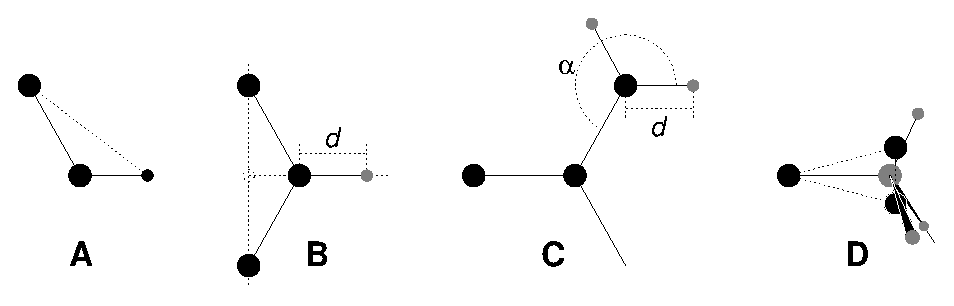
\includegraphics[width=11cm]{plots/dumtypes}}
\caption[Virtual site constructions for hydrogen atoms.]{The different
types of virtual site constructions used for hydrogen atoms. The atoms
used in the construction of the virtual site(s) are depicted as black
circles, virtual sites as gray ones. Hydrogens are smaller than heavy
atoms. {\sf A}: fixed bond angle, note that here the hydrogen is not a
virtual site; {\sf B}: in the plane of three atoms, with fixed distance;
{\sf C}: in the plane of three atoms, with fixed angle and distance;
{\sf D}: construction for amine groups ({\amine} or {\aminep}), see
text for details.}
\label{fig:vsitehydro}
\end{figure}

The goal of defining hydrogen atoms as virtual sites is to remove all
high-frequency degrees of freedom from them. In some cases, not all
degrees of freedom of a hydrogen atom should be removed, {\eg} in the
case of hydroxyl or amine groups the rotational freedom of the
hydrogen atom(s) should be preserved. Care should be taken that no
unwanted correlations are introduced by the construction of virtual
sites, {\eg} bond-angle vibration between the constructing atoms could
translate into hydrogen bond-length vibration. Additionally, since
virtual sites are by definition massless, in order to preserve total
system mass, the mass of each hydrogen atom that is treated as virtual
site should be added to the bonded heavy atom.

Taking into account these considerations, the hydrogen atoms in a
protein naturally fall into several categories, each requiring a
different approach (see also \figref{vsitehydro}).

\begin{itemize}

\item{\em hydroxyl ({\sf -OH}) or sulfhydryl ({\sf -SH})
hydrogen:\/} The only internal degree of freedom in a hydroxyl group
that can be constrained is the bending of the {\sf C-O-H} angle. This
angle is fixed by defining an additional bond of appropriate length,
see \figref{vsitehydro}A. Doing so removes the high-frequency angle bending,
but leaves the dihedral rotational freedom. The same goes for a
sulfhydryl group. {\bf Note} that in these cases the hydrogen is not treated
as a virtual site.

\item{\em single amine or amide ({\amines}) and aromatic hydrogens
({\sf -CH-}):\/} The position of these hydrogens cannot be constructed
from a linear combination of bond vectors, because of the flexibility
of the angle between the heavy atoms. Instead, the hydrogen atom is
positioned at a fixed distance from the bonded heavy atom on a line
going through the bonded heavy atom and a point on the line through
both second bonded atoms, see \figref{vsitehydro}B.

\item{\em planar amine ({\amine}) hydrogens:\/} The method used for
the single amide hydrogen is not well suited for planar amine groups,
because no suitable two heavy atoms can be found to define the
direction of the hydrogen atoms. Instead, the hydrogen is constructed
at a fixed distance from the nitrogen atom, with a fixed angle to the
carbon atom, in the plane defined by one of the other heavy atoms, see
\figref{vsitehydro}C.

\item{\em amine group (umbrella {\amine} or {\aminep}) hydrogens:\/}
Amine hydrogens with rotational freedom cannot be constructed as virtual
sites from the heavy atoms they are connected to, since this would
result in loss of the rotational freedom of the amine group. To
preserve the rotational freedom while removing the hydrogen bond-angle
degrees of freedom, two ``dummy masses'' are constructed with the same
total mass, moment of inertia (for rotation around the {\sf C-N} bond)
and center of mass as the amine group. These dummy masses have no
interaction with any other atom, except for the fact that they are
connected to the carbon and to each other, resulting in a rigid
triangle. From these three particles, the positions of the nitrogen and
hydrogen atoms are constructed as linear combinations of the two
carbon-mass vectors and their outer product, resulting in an amine
group with rotational freedom intact, but without other internal
degrees of freedom. See \figref{vsitehydro}D.

\end{itemize}

\begin{figure}
\centerline{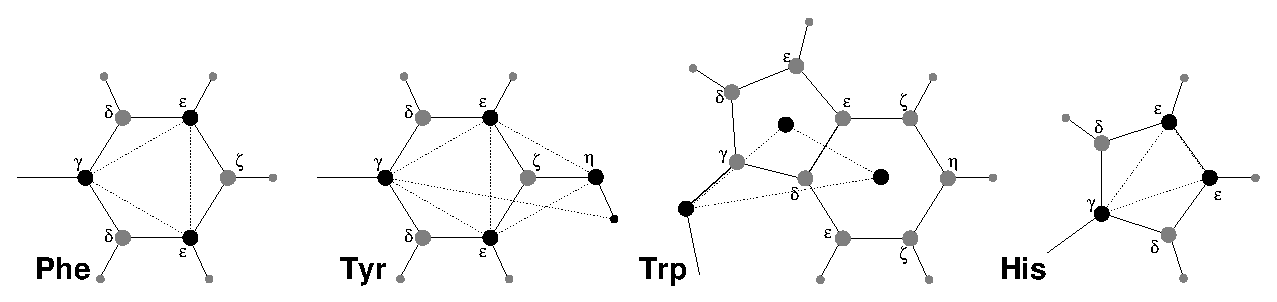
\includegraphics[width=15cm]{plots/dumaro}}
\caption[Virtual site constructions for aromatic residues.]{The
different types of virtual site constructions used for aromatic
residues. The atoms used in the construction of the virtual site(s) are
depicted as black circles, virtual sites as gray ones. Hydrogens are
smaller than heavy atoms. {\sf A}: phenylalanine; {\sf B}: tyrosine
(note that the hydroxyl hydrogen is {\em not} a virtual site); {\sf C}:
tryptophan; {\sf D}: histidine.}
\label{fig:vistearo}
\end{figure}

\subsection{Out-of-plane vibrations in aromatic groups}
\label{sec:vsitearo}
The planar arrangements in the side chains of the aromatic residues
lends itself perfectly to a virtual-site construction, giving a
perfectly planar group without the inherently unstable constraints
that are necessary to keep normal atoms in a plane. The basic approach
is to define three atoms or dummy masses with constraints between them
to fix the geometry and create the rest of the atoms as simple virtual
sites type (see \secref{virtual_sites}) from these three. Each of
the aromatic residues require a different approach:

\begin{itemize}

\item{\em Phenylalanine:\/} {\sf C}$_\gamma$, {\sf C}$_{{\epsilon}1}$,
and {\sf C}$_{{\epsilon}2}$ are kept as normal atoms, but with each a
mass of one third the total mass of the phenyl group. See
\figref{vsitehydro}A.

\item{\em Tyrosine:\/} The ring is treated identically to the
phenylalanine ring. Additionally, constraints are defined between {\sf
C}$_{{\epsilon}1}$, {\sf C}$_{{\epsilon}2}$, and {\sf O}$_{\eta}$.
The original improper dihedral angles will keep both triangles (one
for the ring and one with {\sf O}$_{\eta}$) in a plane, but due to the
larger moments of inertia this construction will be much more
stable. The bond-angle in the hydroxyl group will be constrained by a
constraint between {\sf C}$_\gamma$ and {\sf H}$_{\eta}$. {\bf Note} that
the hydrogen is not treated as a virtual site. See
\figref{vsitehydro}B.

\item{\em Tryptophan:\/} {\sf C}$_\beta$ is kept as a normal atom
and two dummy masses are created at the center of mass of each of the
rings, each with a mass equal to the total mass of the respective ring
({\sf C}$_{{\delta}2}$ and {\sf C}$_{{\epsilon}2}$ are each
counted half for each ring). This keeps the overall center of mass and
the moment of inertia almost (but not quite) equal to what it was. See
\figref{vsitehydro}C.

\item{\em Histidine:\/} {\sf C}$_\gamma$, {\sf C}$_{{\epsilon}1}$
and {\sf N}$_{{\epsilon}2}$ are kept as normal atoms, but with masses
redistributed such that the center of mass of the ring is
preserved. See \figref{vsitehydro}D.

\end{itemize}

\section{Viscosity calculation\index{viscosity}}

The shear viscosity is a property of liquids that can be determined easily  
by experiment. It is useful for parameterizing a force field
because it is a kinetic property, while most other properties
which are used for parameterization are thermodynamic.
The viscosity is also an important property, since it influences
the rates of conformational changes of molecules solvated in the liquid.

The viscosity can be calculated from an equilibrium simulation using
an Einstein relation:
\beq
\eta = \frac{1}{2}\frac{V}{k_B T} \lim_{t \rightarrow \infty}
\frac{\mbox{d}}{\mbox{d} t} \left\langle 
\left( \int_{t_0}^{{t_0}+t} P_{xz}(t') \mbox{d} t' \right)^2
\right\rangle_{t_0}
\eeq
This can be done with {\tt gmx energy}.
This method converges very slowly~\cite{Hess2002a}, and as such
a nanosecond simulation might not
be long enough for an accurate determination of the viscosity.
The result is very dependent on the treatment of the electrostatics.
Using a (short) cut-off results in large noise on the off-diagonal
pressure elements, which can increase the calculated viscosity by an order
of magnitude.

{\gromacs} also has a non-equilibrium method for determining
the viscosity~\cite{Hess2002a}.
This makes use of the fact that energy, which is fed into system by
external forces, is dissipated through viscous friction. The generated heat
is removed by coupling to a heat bath. For a Newtonian liquid adding a 
small force will result in a velocity gradient according to the following
equation:
\beq
a_x(z) + \frac{\eta}{\rho} \frac{\partial^2 v_x(z)}{\partial z^2} = 0
\eeq
Here we have applied an acceleration $a_x(z)$ in the $x$-direction, which
is a function of the $z$-coordinate.
In {\gromacs} the acceleration profile is:
\beq
a_x(z) = A \cos\left(\frac{2\pi z}{l_z}\right)
\eeq
where $l_z$ is the height of the box. The generated velocity profile is:
\beq
v_x(z) = V \cos\left(\frac{2\pi z}{l_z}\right)
\eeq
\beq
V = A \frac{\rho}{\eta}\left(\frac{l_z}{2\pi}\right)^2
\eeq
The viscosity can be calculated from $A$ and $V$:
\beq
\label{visc}
\eta = \frac{A}{V}\rho \left(\frac{l_z}{2\pi}\right)^2
\eeq

In the simulation $V$ is defined as:
\beq
V = \frac{\displaystyle \sum_{i=1}^N m_i v_{i,x} 2 \cos\left(\frac{2\pi z}{l_z}\right)}
         {\displaystyle \sum_{i=1}^N m_i}
\eeq
The generated velocity profile is not coupled to the heat bath. Moreover,
the velocity profile is excluded from the kinetic energy.
One would like $V$ to be as large as possible to get good statistics.
However, the shear rate should not be so high that the system gets too far
from equilibrium. The maximum shear rate occurs where the cosine is zero,
the rate being:
\beq
\mbox{sh}_{\max} =  \max_z \left| \frac{\partial v_x(z)}{\partial z} \right|
= A \frac{\rho}{\eta} \frac{l_z}{2\pi}
\eeq
For a simulation with: $\eta=10^{-3}$ [kg\,m$^{-1}$\,s$^{-1}$],
$\rho=10^3$\,[kg\,m$^{-3}$] and $l_z=2\pi$\,[nm],
$\mbox{sh}_{\max}=1$\,[ps\,nm$^{-1}$] $A$.
This shear rate should be smaller than one over the longest
correlation time in the system. For most liquids, this will be the rotation
correlation time, which is around 10 ps. In this case, $A$ should
be smaller than 0.1\,[nm\,ps$^{-2}$].
When the shear rate is too high, the observed viscosity will be too low.
Because $V$ is proportional to the square of the box height,
the optimal box is elongated in the $z$-direction.
In general, a simulation length of 100 ps is enough to obtain an
accurate value for the viscosity.

The heat generated by the viscous friction is removed by coupling to a heat
bath. Because this coupling is not instantaneous the real temperature of the
liquid will be slightly lower than the observed temperature.
Berendsen derived this temperature shift~\cite{Berendsen91}, which can
be written in terms of the shear rate as:
\beq
T_s = \frac{\eta\,\tau}{2 \rho\,C_v} \mbox{sh}_{\max}^2
\eeq
where $\tau$ is the coupling time for the Berendsen thermostat and
$C_v$ is the heat capacity. Using the values of the example above,
$\tau=10^{-13}$ [s] and $C_v=2 \cdot 10^3$\,[J kg$^{-1}$\,K$^{-1}$], we
get: $T_s=25$\,[K\,ps$^{-2}$]\,sh$_{\max}^2$. When we want the shear
rate to be smaller than $1/10$\,[ps$^{-1}$], $T_s$ is smaller than
0.25\,[K], which is negligible.

{\bf Note} that the system has to build up the velocity profile when starting
from an equilibrium state. This build-up time is of the order of the
correlation time of the liquid.

Two quantities are written to the energy file, along with their averages
and fluctuations: $V$ and $1/\eta$, as obtained from (\ref{visc}).

\section{Tabulated interaction functions\index{tabulated interaction functions}}
\subsection{Cubic splines for potentials}
\label{subsec:cubicspline}
In some of the inner loops of {\gromacs}, look-up tables are used 
for computation of potential and forces. 
The tables are interpolated using a cubic
spline algorithm. 
There are separate tables for electrostatic, dispersion, and repulsion
interactions,
but for the sake of caching performance these have been combined
into a single array. 
The cubic spline interpolation for $x_i \leq x < x_{i+1}$ looks like this:
\beq
V_s(x) = A_0 + A_1 \,\epsilon + A_2 \,\epsilon^2 + A_3 \,\epsilon^3
\label{eqn:spline}
\eeq
where the table spacing $h$ and fraction $\epsilon$ are given by:
\bea
h	&=&	x_{i+1} - x_i	\\
\epsilon&=&	(x - x_i)/h
\eea
so that $0 \le \epsilon < 1$.
From this, we can calculate the derivative in order to determine the forces:
\beq
-V_s'(x) ~=~ 
-\frac{{\rm d}V_s(x)}{{\rm d}\epsilon}\frac{{\rm d}\epsilon}{{\rm d}x} ~=~
-(A_1 + 2 A_2 \,\epsilon + 3 A_3 \,\epsilon^2)/h
\eeq
The four coefficients are determined from the four conditions
that $V_s$ and $-V_s'$ at both ends of each interval should match
the exact potential $V$ and force $-V'$.
This results in the following errors for each interval:
\bea
|V_s  - V  |_{max} &=& V'''' \frac{h^4}{384} + O(h^5) \\
|V_s' - V' |_{max} &=& V'''' \frac{h^3}{72\sqrt{3}} + O(h^4) \\
|V_s''- V''|_{max} &=& V'''' \frac{h^2}{12}  + O(h^3)
\eea
V and V' are continuous, while V'' is the first discontinuous
derivative.
The number of points per nanometer is 500 and 2000
for mixed- and double-precision versions of {\gromacs}, respectively.
This means that the errors in the potential and force will usually
be smaller than the mixed precision accuracy.

{\gromacs} stores $A_0$, $A_1$, $A_2$ and $A_3$.
The force routines get a table with these four parameters and
a scaling factor $s$ that is equal to the number of points per nm.
({\bf Note} that $h$ is $s^{-1}$).
The algorithm goes a little something like this:
\begin{enumerate}
\item	Calculate distance vector (\ve{r}$_{ij}$) and distance r$_{ij}$
\item	Multiply r$_{ij}$ by $s$ and truncate to an integer value $n_0$
	to get a table index
\item	Calculate fractional component ($\epsilon$ = $s$r$_{ij} - n_0$) 
	and $\epsilon^2$ 
\item	Do the interpolation to calculate the potential $V$ and the scalar force $f$
\item	Calculate the vector force \ve{F} by multiplying $f$ with \ve{r}$_{ij}$
\end{enumerate}

{\bf Note} that table look-up is significantly {\em
slower} than computation of the most simple Lennard-Jones and Coulomb
interaction. However, it is much faster than the shifted Coulomb
function used in conjunction with the PPPM method. Finally, it is much
easier to modify a table for the potential (and get a graphical
representation of it) than to modify the inner loops of the MD
program.

\subsection{User-specified potential functions}
\label{subsec:userpot}
You can also use your own potential functions\index{potential function} without 
editing the {\gromacs} code.  The potential function should be according to the 
following equation
\beq
V(r_{ij}) ~=~ \frac{q_i q_j}{4 \pi\epsilon_0} f(r_{ij}) + C_6 \,g(r_{ij}) + C_{12} \,h(r_{ij})
\eeq
where $f$, $g$, and $h$ are user defined functions. {\bf Note} that if $g(r)$ represents a
normal dispersion interaction, $g(r)$ should be $<$ 0. C$_6$, C$_{12}$
and the charges are read from the topology. Also note that combination
rules are only supported for Lennard-Jones and Buckingham, and that
your tables should match the parameters in the binary topology.

When you add the following lines in your {\tt .mdp} file:

{\small
\begin{verbatim}
rlist           = 1.0
coulombtype     = User
rcoulomb        = 1.0
vdwtype         = User
rvdw            = 1.0
\end{verbatim}}

{\tt mdrun} will read a single non-bonded table file,
or multiple when {\tt energygrp-table} is set (see below).
The name of the file(s) can be set with the {\tt mdrun} option {\tt -table}.
The table file should contain seven columns of table look-up data in the
order: $x$, $f(x)$, $-f'(x)$, $g(x)$, $-g'(x)$, $h(x)$, $-h'(x)$.
The $x$ should run from 0 to $r_c+1$ (the value of {\tt table_extension} can be
changed in the {\tt .mdp} file).
You can choose the spacing you like; for the standard tables {\gromacs}
uses a spacing of 0.002 and 0.0005 nm when you run in mixed
and double precision, respectively.  In this
context, $r_c$ denotes the maximum of the two cut-offs {\tt rvdw} and
{\tt rcoulomb} (see above). These variables need not be the same (and
need not be 1.0 either).  Some functions used for potentials contain a
singularity at $x = 0$, but since atoms are normally not closer to each
other than 0.1 nm, the function value at $x = 0$ is not important.
Finally, it is also
possible to combine a standard Coulomb with a modified LJ potential
(or vice versa). One then specifies {\eg} {\tt coulombtype = Cut-off} or
{\tt coulombtype = PME}, combined with {\tt vdwtype = User}.  The table file must
always contain the 7 columns however, and meaningful data (i.e. not
zeroes) must be entered in all columns.  A number of pre-built table
files can be found in the {\tt GMXLIB} directory for 6-8, 6-9, 6-10, 6-11, and 6-12
Lennard-Jones potentials combined with a normal Coulomb.

If you want to have different functional forms between different
groups of atoms, this can be set through energy groups.
Different tables can be used for non-bonded interactions between
different energy groups pairs through the {\tt .mdp} option {\tt energygrp-table}
(see details in the User Guide).
Atoms that should interact with a different potential should
be put into different energy groups.
Between group pairs which are not listed in {\tt energygrp-table},
the normal user tables will be used. This makes it easy to use
a different functional form between a few types of atoms.

\section{Mixed Quantum-Classical simulation techniques}

In a molecular mechanics (MM) force field, the influence of electrons
is expressed by empirical parameters that are assigned on the basis of
experimental data, or on the basis of results from high-level quantum
chemistry calculations. These are valid for the ground state of a
given covalent structure, and the MM approximation is usually
sufficiently accurate for ground-state processes in which the overall
connectivity between the atoms in the system remains
unchanged. However, for processes in which the connectivity does
change, such as chemical reactions, or processes that involve multiple
electronic states, such as photochemical conversions, electrons can no
longer be ignored, and a quantum mechanical description is required
for at least those parts of the system in which the reaction takes
place.

One approach to the simulation of chemical reactions in solution, or
in enzymes, is to use a combination of quantum mechanics (QM) and
molecular mechanics (MM). The reacting parts of the system are treated
quantum mechanically, with the remainder being modeled using the
force field. The current version of {\gromacs} provides interfaces to
several popular Quantum Chemistry packages (MOPAC~\cite{mopac},
GAMESS-UK~\cite{gamess-uk}, Gaussian~\cite{g03} and CPMD~\cite{Car85a}).

{\gromacs} interactions between the two subsystems are
either handled as described by Field {\em et al.}~\cite{Field90a} or
within the ONIOM approach by Morokuma and coworkers~\cite{Maseras96a,
Svensson96a}.

\subsection{Overview}

Two approaches for describing the interactions between the QM and MM
subsystems are supported in this version:

\begin{enumerate}
\item{\textbf{Electronic Embedding}} The electrostatic interactions
between the electrons of the QM region and the MM atoms and between
the QM nuclei and the MM atoms are included in the Hamiltonian for
the QM subsystem: \beq H^{QM/MM} =
H^{QM}_e-\sum_i^n\sum_J^M\frac{e^2Q_J}{4\pi\epsilon_0r_{iJ}}+\sum_A^N\sum_J^M\frac{e^2Z_AQ_J}{e\pi\epsilon_0R_{AJ}},
\eeq where $n$ and $N$ are the number of electrons and nuclei in the
QM region, respectively, and $M$ is the number of charged MM
atoms. The first term on the right hand side is the original
electronic Hamiltonian of an isolated QM system. The first of the
double sums is the total electrostatic interaction between the QM
electrons and the MM atoms. The total electrostatic interaction of the
QM nuclei with the MM atoms is given by the second double sum. Bonded
interactions between QM and MM atoms are described at the MM level by
the appropriate force-field terms. Chemical bonds that connect the two
subsystems are capped by a hydrogen atom to complete the valence of
the QM region. The force on this atom, which is present in the QM
region only, is distributed over the two atoms of the bond. The cap
atom is usually referred to as a link atom.

\item{\textbf{ONIOM}} In the ONIOM approach, the energy and gradients
are first evaluated for the isolated QM subsystem at the desired level
of {\it{ab initio}} theory. Subsequently, the energy and gradients of
the total system, including the QM region, are computed using the
molecular mechanics force field and added to the energy and gradients
calculated for the isolated QM subsystem. Finally, in order to correct
for counting the interactions inside the QM region twice, a molecular
mechanics calculation is performed on the isolated QM subsystem and
the energy and gradients are subtracted. This leads to the following
expression for the total QM/MM energy (and gradients likewise): \beq
E_{tot} = E_{I}^{QM}
+E_{I+II}^{MM}-E_{I}^{MM}, \eeq where the
subscripts I and II refer to the QM and MM subsystems,
respectively. The superscripts indicate at what level of theory the
energies are computed. The ONIOM scheme has the
advantage that it is not restricted to a two-layer QM/MM description,
but can easily handle more than two layers, with each layer described
at a different level of theory.
\end{enumerate}

\subsection{Usage}

To make use of the QM/MM functionality in {\gromacs}, one needs to:

\begin{enumerate}
\item introduce link atoms at the QM/MM boundary, if needed;
\item specify which atoms are to be treated at a QM level;
\item specify the QM level, basis set, type of QM/MM interface and so on. 
\end{enumerate}

\subsubsection{Adding link atoms}

At the bond that connects the QM and MM subsystems, a link atoms is
introduced.  In {\gromacs} the link atom has special atomtype, called
LA. This atomtype is treated as a hydrogen atom in the QM calculation,
and as a virtual site in the force-field calculation. The link atoms, if
any, are part of the system, but have no interaction with any other
atom, except that the QM force working on it is distributed over the
two atoms of the bond. In the topology, the link atom (LA), therefore,
is defined as a virtual site atom:

{\small
\begin{verbatim}
[ virtual_sites2 ]
LA QMatom MMatom 1 0.65
\end{verbatim}}

See~\secref{vsitetop} for more details on how virtual sites are
treated. The link atom is replaced at every step of the simulation.

In addition, the bond itself is replaced by a constraint:

{\small
\begin{verbatim}
[ constraints ]
QMatom MMatom 2 0.153
\end{verbatim}}

{\bf Note} that, because in our system the QM/MM bond is a carbon-carbon
bond (0.153 nm), we use a constraint length of 0.153 nm, and dummy
position of 0.65. The latter is the ratio between the ideal C-H
bond length and the ideal C-C bond length. With this ratio, the link
atom is always 0.1 nm away from the {\tt QMatom}, consistent with the
carbon-hydrogen bond length. If the QM and MM subsystems are connected
by a different kind of bond, a different constraint and a different
dummy position, appropriate for that bond type, are required.

\subsubsection{Specifying the QM atoms}

Atoms that should be treated at a QM level of theory, including the
link atoms, are added to the index file. In addition, the chemical
bonds between the atoms in the QM region are to be defined as
connect bonds (bond type 5) in the topology file:

{\small
\begin{verbatim}
[ bonds ]
QMatom1 QMatom2 5
QMatom2 QMatom3 5
\end{verbatim}}

\subsubsection{Specifying the QM/MM simulation parameters}

In the {\tt .mdp} file, the following parameters control a QM/MM simulation.

\begin{description}

\item[\tt QMMM = no]\mbox{}\\ If this is set to {\tt yes}, a QM/MM
simulation is requested. Several groups of atoms can be described at
different QM levels separately. These are specified in the QMMM-grps
field separated by spaces. The level of {\it{ab initio}} theory at which the
groups are described is specified by {\tt QMmethod} and {\tt QMbasis}
Fields. Describing the groups at different levels of theory is only
possible with the ONIOM QM/MM scheme, specified by {\tt QMMMscheme}.

\item[\tt QMMM-grps =]\mbox{}\\groups to be described at the QM level

\item[\tt QMMMscheme = normal]\mbox{}\\Options are {\tt normal} and
{\tt ONIOM}. This selects the QM/MM interface. {\tt normal} implies
that the QM subsystem is electronically embedded in the MM
subsystem. There can only be one {\tt QMMM-grps} that is modeled at
the {\tt QMmethod} and {\tt QMbasis} level of {\it{ ab initio}}
theory. The rest of the system is described at the MM level. The QM
and MM subsystems interact as follows: MM point charges are included
in the QM one-electron Hamiltonian and all Lennard-Jones interactions
are described at the MM level. If {\tt ONIOM} is selected, the
interaction between the subsystem is described using the ONIOM method
by Morokuma and co-workers. There can be more than one QMMM-grps each
modeled at a different level of QM theory (QMmethod and QMbasis).

\item[\tt QMmethod = ]\mbox{}\\Method used to compute the energy
and gradients on the QM atoms. Available methods are AM1, PM3, RHF,
UHF, DFT, B3LYP, MP2, CASSCF, MMVB and CPMD. For CASSCF, the number of
electrons and orbitals included in the active space is specified by
{\tt CASelectrons} and {\tt CASorbitals}. For CPMD, the plane-wave
cut-off is specified by the {\tt planewavecutoff} keyword.

\item[\tt QMbasis = ]\mbox{}\\Gaussian basis set used to expand the
electronic wave-function. Only Gaussian basis sets are currently
available, i.e. STO-3G, 3-21G, 3-21G*, 3-21+G*, 6-21G, 6-31G, 6-31G*,
6-31+G*, and 6-311G. For CPMD, which uses plane wave expansion rather
than atom-centered basis functions, the {\tt planewavecutoff} keyword
controls the plane wave expansion.

\item[\tt QMcharge = ]\mbox{}\\The total charge in {\it{e}} of the {\tt
QMMM-grps}. In case there are more than one {\tt QMMM-grps}, the total
charge of each ONIOM layer needs to be specified separately.

\item[\tt QMmult = ]\mbox{}\\The multiplicity of the {\tt
QMMM-grps}. In case there are more than one {\tt QMMM-grps}, the
multiplicity of each ONIOM layer needs to be specified separately.

\item[\tt CASorbitals = ]\mbox{}\\The number of orbitals to be
included in the active space when doing a CASSCF computation.

\item[\tt CASelectrons = ]\mbox{}\\The number of electrons to be
included in the active space when doing a CASSCF computation.

\item[\tt SH = no]\mbox{}\\If this is set to yes, a QM/MM MD
simulation on the excited state-potential energy surface and enforce a
diabatic hop to the ground-state when the system hits the conical
intersection hyperline in the course the simulation. This option only
works in combination with the CASSCF method.

\end{description}

\subsection{Output}

The energies and gradients computed in the QM calculation are added to
those computed by {\gromacs}. In the {\tt .edr} file there is a section
for the total QM energy.

\subsection{Future developments}

Several features are currently under development to increase the
accuracy of the QM/MM interface. One useful feature is the use of
delocalized MM charges in the QM computations. The most important
benefit of using such smeared-out charges is that the Coulombic
potential has a finite value at interatomic distances. In the point
charge representation, the partially-charged MM atoms close to the QM
region tend to ``over-polarize'' the QM system, which leads to artifacts
in the calculation.

What is needed as well is a transition state optimizer.

\section{Using VMD plug-ins for trajectory file I/O}
\index{VMD plug-ins}\index{trajectory file}{\gromacs} tools are able
to use the plug-ins found in an existing installation of
\href{http://www.ks.uiuc.edu/Research/vmd}{VMD} in order to read and
write trajectory files in formats that are not native to
{\gromacs}. You will be able to supply an AMBER DCD-format trajectory
filename directly to {\gromacs} tools, for example.

This requires a VMD installation not older than version 1.8, that your
system provides the dlopen function so that programs can determine at
run time what plug-ins exist, and that you build shared libraries when
building {\gromacs}. CMake will find the vmd executable in your path, and
from it, or the environment variable {\tt VMDDIR} at configuration or
run time, locate the plug-ins. Alternatively, the {\tt VMD_PLUGIN_PATH}
can be used at run time to specify a path where these plug-ins can be
found. Note that these plug-ins are in a binary format, and that format
must match the architecture of the machine attempting to use them.


\section{\normindex{Interactive Molecular Dynamics}}
{\gromacs} supports the interactive molecular dynamics (IMD) protocol as implemented
by \href{http://www.ks.uiuc.edu/Research/vmd}{VMD} to control a running simulation
in NAMD. IMD allows to monitor a running {\gromacs} simulation from a VMD client.
In addition, the user can interact with the simulation by pulling on atoms, residues
or fragments with a mouse or a force-feedback device. Additional information about
the {\gromacs} implementation and an exemplary {\gromacs} IMD system can be found
\href{http://www.mpibpc.mpg.de/grubmueller/interactivemd}{on this homepage}.

\subsection{Simulation input preparation}
The {\gromacs} implementation allows transmission and interaction with a part of the
running simulation only, e.g.\ in cases where no water molecules should be transmitted
or pulled. The group is specified via the {\tt .mdp} option {\tt IMD-group}. When
{\tt IMD-group} is empty, the IMD protocol is disabled and cannot be enabled via the
switches in {\tt mdrun}. To interact with the entire system, {\tt IMD-group} can
be set to {\tt System}. When using {\tt grompp}, a {\tt .gro} file
to be used as VMD input is written out ({\tt -imd} switch of {\tt grompp}).

\subsection{Starting the simulation}
Communication between VMD and {\gromacs} is achieved via TCP sockets and thus enables
controlling an {\tt mdrun} running locally or on a remote cluster. The port for the
connection can be specified with the {\tt -imdport} switch of {\tt mdrun}, 8888 is
the default. If a port number of 0 or smaller is provided, {\gromacs} automatically
assigns a free port to use with IMD.

Every $N$ steps, the {\tt mdrun} client receives the applied forces from VMD and sends the new
positions to the client. VMD permits increasing or decreasing the communication frequency
interactively.
By default, the simulation starts and runs even if no IMD client is connected. This
behavior is changed by the {\tt -imdwait} switch of {\tt mdrun}. After startup and
whenever the client has disconnected, the integration stops until reconnection of
the client.
When the {\tt -imdterm} switch is used, the simulation can be terminated by pressing
the stop button in VMD. This is disabled by default.
Finally, to allow interacting with the simulation (i.e. pulling from VMD) the {\tt -imdpull}
switch has to be used.
Therefore, a simulation can only be monitored but not influenced from the VMD client
when none of {\tt -imdwait}, {\tt -imdterm} or {\tt -imdpull} are set. However, since
the IMD protocol requires no authentication, it is not advisable to run simulations on
a host directly reachable from an insecure environment. Secure shell forwarding of TCP
can be used to connect to running simulations not directly reachable from the interacting host.
Note that the IMD command line switches of {\tt mdrun} are hidden by default and show
up in the help text only with {\tt gmx mdrun -h -hidden}.

\subsection{Connecting from VMD}
In VMD, first the structure corresponding to the IMD group has to be loaded ({\it File
$\rightarrow$ New Molecule}). Then the IMD connection window has to be used
({\it Extensions $\rightarrow$ Simulation $\rightarrow$ IMD Connect (NAMD)}). In the IMD
connection window, hostname and port have to be specified and followed by pressing
{\it Connect}. {\it Detach Sim} allows disconnecting without terminating the simulation, while
{\it Stop Sim} ends the simulation on the next neighbor searching step (if allowed by
{\tt -imdterm}).

The timestep transfer rate allows adjusting the communication frequency between simulation
and IMD client. Setting the keep rate loads every $N^\mathrm{th}$ frame into VMD instead
of discarding them when a new one is received. The displayed energies are in SI units
in contrast to energies displayed from NAMD simulations.

\section{\normindex{Embedding proteins into the membranes}}
\label{sec:membed}

GROMACS is capable of inserting the protein into pre-equilibrated
lipid bilayers with minimal perturbation of the lipids using the
method, which was initially described as a ProtSqueeze
technique,\cite{Yesylevskyy2007} and later implemented as g\_membed
tool.\cite{Wolf2010} Currently the functionality of g\_membed is
available in mdrun as described in the user guide.

This method works by first artificially shrinking the protein in the
$xy$-plane, then it removes lipids that overlap with that much smaller
core. Then the protein atoms are gradually resized back to their
initial configuration, using normal dynamics for the rest of the
system, so the lipids adapt to the protein. Further lipids are removed
as required.


% LocalWords:  PMF pmf kJ mol Jarzynski BT bilayer rup mdp AFM fepmf fecalc rb
% LocalWords:  posre grompp fs Verlet dihedrals hydrogens hydroxyl sulfhydryl
% LocalWords:  vsitehydro planarity chirality pdb gmx virtualize virtualized xz
% LocalWords:  vis massless tryptophan histidine phenyl parameterizing ij PPPM
% LocalWords:  parameterization Berendsen rlist coulombtype rcoulomb vdwtype LJ
% LocalWords:  rvdw energygrp mdrun pre GMXLIB MOPAC GAMESS CPMD ONIOM
% LocalWords:  Morokuma iJ AQ AJ initio atomtype QMatom MMatom QMMM grps et al
% LocalWords:  QMmethod QMbasis QMMMscheme RHF DFT LYP CASSCF MMVB CASelectrons
% LocalWords:  CASorbitals planewavecutoff STO QMcharge QMmult diabatic edr
% LocalWords:  hyperline delocalized Coulombic indices nm ccc th ps
% LocalWords:  GTX CPUs GHz md sd bd vv avek tcoupl andersen tc OPLSAA GROMOS
% LocalWords:  OBC obc CCMA tol pbc xyz barostat pcoupl acc gpu PLUGIN Cmake GX
% LocalWords:  MSVC gcc installpath cmake DGMX DCMAKE functionalities GPGPU GTS
% LocalWords:  OpenCL DeviceID gromacs gpus html GeForce Quadro FX Plex CX GF
% LocalWords:  VMD DCD GROningen MAchine BIOSON Groningen der Spoel Drunen Comp
% LocalWords:  Phys Comm moltype intramol vdw Waals fep multivector pf
% LocalWords:  pymbar dhdl xvg LINCS Entropic entropic solutes ref com iso pm
% LocalWords:  rm prefactors equipotential potiso potisopf potpm trr
% LocalWords:  potrm potrmpf midplanes midplane gaussians potflex vars massw av
% LocalWords:  shure observables rccccccc vec eps dist min eqn transl nstsout
% LocalWords:  nstrout rotangles rotslabs rottorque RMSD rmsdfit excl NH amine
% LocalWords:  positionrestraint es SH phenylalanine solvated sh nanometer QM
% LocalWords:  Lennard Buckingham UK Svensson ab vsitetop co UHF MP interatomic
% LocalWords:  cg grp coords SPC userpot
% LocalWords:  itp sitesn atomtypes ff csg ndx Tesla CHARMM AA gauss
% LocalWords:  CMAP nocmap fators Monte performant lib LD DIR llllcc
% LocalWords:  CMake homepage DEV overclocking GT dlopen vmd VMDDIR
% LocalWords:  versa PME atomperatom graining forcefields hy spc OPLS
% LocalWords:  topol multi

%
% This file is part of the GROMACS molecular simulation package.
%
% Copyright (c) 2013,2014,2015,2016, by the GROMACS development team, led by
% Mark Abraham, David van der Spoel, Berk Hess, and Erik Lindahl,
% and including many others, as listed in the AUTHORS file in the
% top-level source directory and at http://www.gromacs.org.
%
% GROMACS is free software; you can redistribute it and/or
% modify it under the terms of the GNU Lesser General Public License
% as published by the Free Software Foundation; either version 2.1
% of the License, or (at your option) any later version.
%
% GROMACS is distributed in the hope that it will be useful,
% but WITHOUT ANY WARRANTY; without even the implied warranty of
% MERCHANTABILITY or FITNESS FOR A PARTICULAR PURPOSE.  See the GNU
% Lesser General Public License for more details.
%
% You should have received a copy of the GNU Lesser General Public
% License along with GROMACS; if not, see
% http://www.gnu.org/licenses, or write to the Free Software Foundation,
% Inc., 51 Franklin Street, Fifth Floor, Boston, MA  02110-1301  USA.
%
% If you want to redistribute modifications to GROMACS, please
% consider that scientific software is very special. Version
% control is crucial - bugs must be traceable. We will be happy to
% consider code for inclusion in the official distribution, but
% derived work must not be called official GROMACS. Details are found
% in the README & COPYING files - if they are missing, get the
% official version at http://www.gromacs.org.
%
% To help us fund GROMACS development, we humbly ask that you cite
% the research papers on the package. Check out http://www.gromacs.org.

\chapter{Run parameters and Programs}
\label{ch:programs}

\section{Online documentation}
\index{online documentation}
More documentation is available online from the {\gromacs} web site,
\url{http://manual.gromacs.org/documentation}.

In addition, we install standard UNIX man pages for all the programs. If
you have sourced the {\tt GMXRC} script in the {\gromacs} binary directory for
your host they should already be present in your {\tt MANPATH} environment variable, and you
should be able to type {\eg} {\tt man gmx-grompp}. You can also use
the {\tt -h} flag on the command line (e.g. {\tt gmx grompp -h}) to
see the same information, as well as {\tt gmx help grompp}.
The list of all programs are available from {\tt gmx help}.

\section{File types\swapindexquiet{file}{type}}
\label{sec:fileformats}
\tabref{form} lists the file types used by {\gromacs} along with
a short description, and you can find a more detail description for
each file in your HTML reference, or in our online version.

{\gromacs} files written in \normindex{XDR} format can be read on any
architecture with {\gromacs} version 1.6 or later if the configuration
script found the XDR libraries on your system. They should always be
present on UNIX since they are necessary for NFS support.

%
% This file is part of the GROMACS molecular simulation package.
%
% Copyright (c) 2013,2014,2015, by the GROMACS development team, led by
% Mark Abraham, David van der Spoel, Berk Hess, and Erik Lindahl,
% and including many others, as listed in the AUTHORS file in the
% top-level source directory and at http://www.gromacs.org.
%
% GROMACS is free software; you can redistribute it and/or
% modify it under the terms of the GNU Lesser General Public License
% as published by the Free Software Foundation; either version 2.1
% of the License, or (at your option) any later version.
%
% GROMACS is distributed in the hope that it will be useful,
% but WITHOUT ANY WARRANTY; without even the implied warranty of
% MERCHANTABILITY or FITNESS FOR A PARTICULAR PURPOSE.  See the GNU
% Lesser General Public License for more details.
%
% You should have received a copy of the GNU Lesser General Public
% License along with GROMACS; if not, see
% http://www.gnu.org/licenses, or write to the Free Software Foundation,
% Inc., 51 Franklin Street, Fifth Floor, Boston, MA  02110-1301  USA.
%
% If you want to redistribute modifications to GROMACS, please
% consider that scientific software is very special. Version
% control is crucial - bugs must be traceable. We will be happy to
% consider code for inclusion in the official distribution, but
% derived work must not be called official GROMACS. Details are found
% in the README & COPYING files - if they are missing, get the
% official version at http://www.gromacs.org.
%
% To help us fund GROMACS development, we humbly ask that you cite
% the research papers on the package. Check out http://www.gromacs.org.

% TODO generate this from the code!
\begin{table}
\begin{tabularx}{\linewidth}{|r@{\tt.}lccX|}
\dline
\mc{2}{|c}{Default} &      & Default &  \\[-0.1ex]
\mc{1}{|c}{Name} & \mc{1}{c}{Ext.} & Type &  Option & Description \\[-0.1ex]
\hline
\tt   atomtp & \tt atp & Asc & \tt    & Atomtype file used by {\tt pdb2gmx} \\[-0.1ex]
\tt    eiwit & \tt brk & Asc & \tt -f & Brookhaven data bank file \\[-0.1ex]
\tt    state & \tt cpt & xdr & \tt    & Checkpoint file \\[-0.1ex]
\tt   nnnice & \tt dat & Asc & \tt    & Generic data file \\[-0.1ex]
\tt     user & \tt dlg & Asc & \tt    & Dialog Box data for {\tt ngmx} \\[-0.1ex]
\tt      sam & \tt edi & Asc & \tt    & ED sampling input \\[-0.1ex]
\tt      sam & \tt edo & Asc & \tt    & ED sampling output \\[-0.1ex]
\tt     ener & \tt edr &     & \tt    & Generic energy: \tt edr ene \\[-0.1ex]
\tt     ener & \tt edr & xdr & \tt    & Energy file in portable xdr format \\[-0.1ex]
\tt     ener & \tt ene & Bin & \tt    & Energy file \\[-0.1ex]
\tt    eiwit & \tt ent & Asc & \tt -f & Entry in the protein date bank \\[-0.1ex]
\tt     plot & \tt eps & Asc & \tt    & Encapsulated PostScript (tm) file \\[-0.1ex]
\tt     conf & \tt esp & Asc & \tt -c & Coordinate file in ESPResSo format \\[-0.1ex]
\tt     conf & \tt g96 & Asc & \tt -c & Coordinate file in Gromos-96 format \\[-0.1ex]
\tt     conf & \tt gro & Asc & \tt -c & Coordinate file in Gromos-87 format \\[-0.1ex]
\tt     conf & \tt gro &     & \tt -c & Structure: \tt gro g96 pdb esp tpr \\[-0.1ex]
\tt      out & \tt gro &     & \tt -o & Structure: \tt gro g96 pdb esp \\[-0.1ex]
\tt    polar & \tt hdb & Asc & \tt    & Hydrogen data base \\[-0.1ex]
\tt   topinc & \tt itp & Asc & \tt    & Include file for topology \\[-0.1ex]
\tt      run & \tt log & Asc & \tt -l & Log file \\[-0.1ex]
\tt       ps & \tt m2p & Asc & \tt    & Input file for mat2ps \\[-0.1ex]
\tt       ss & \tt map & Asc & \tt    & File that maps matrix data to colors \\[-0.1ex]
\tt       ss & \tt mat & Asc & \tt    & Matrix Data file \\[-0.1ex]
\tt   grompp & \tt mdp & Asc & \tt -f & {\tt grompp} input file with MD parameters \\[-0.1ex]
\tt  hessian & \tt mtx & Bin & \tt -m & Hessian matrix \\[-0.1ex]
\tt    index & \tt ndx & Asc & \tt -n & Index file \\[-0.1ex]
\tt    hello & \tt out & Asc & \tt -o & Generic output file \\[-0.1ex]
\tt    eiwit & \tt pdb & Asc & \tt -f & Protein data bank file \\[-0.1ex]
\tt  residue & \tt rtp & Asc & \tt    & Residue Type file used by {\tt pdb2gmx} \\[-0.1ex]
\tt      doc & \tt tex & Asc & \tt -o & LaTeX file \\[-0.1ex]
\tt    topol & \tt top & Asc & \tt -p & Topology file \\[-0.1ex]
\tt    topol & \tt tpr &     & \tt -s & Generic run input: \tt tpr \\[-0.1ex]
\tt    topol & \tt tpr &     & \tt -s & Structure+mass(db): \tt tpr gro g96 pdb \\[-0.1ex]
\tt    topol & \tt tpr & xdr & \tt -s & Portable xdr run input file \\[-0.1ex]
\tt     traj & \tt trr &     & \tt    & Full precision trajectory: \tt trr cpt \\[-0.1ex]
\tt     traj & \tt trr & xdr & \tt    & Trajectory in portable xdr format \\[-0.1ex]
\tt     root & \tt xpm & Asc & \tt    & X PixMap compatible matrix file \\[-0.1ex]
\tt     traj & \tt xtc &     & \tt -f & Trajec., input: \tt xtc trr tng cpt gro g96 pdb \\[-0.1ex]
\tt     traj & \tt xtc &     & \tt -f & Trajectory, output: \tt xtc trr tng gro g96 pdb \\[-0.1ex]
\tt     traj & \tt xtc & xdr & \tt    & Compressed trajectory (portable xdr format) \\[-0.1ex]
\tt    graph & \tt xvg & Asc & \tt -o & xvgr/xmgr file \\[-0.1ex]
\dline
\end{tabularx}
\caption{The {\gromacs} file types.}
\label{tab:form}
\end{table}

% LocalWords:  lccX atomtp atp Asc Atomtype pdb gmx eiwit brk Brookhaven cpt tm
% LocalWords:  xdr nnnice dat dlg ngmx sam edi edo ener edr ene ent eps conf ss
% LocalWords:  PostScript ESPResSo gtraj Gromos gro tpr hdb topinc itp
% LocalWords:  grompp mdp mtx ndx rtp tex LaTeX topol traj trr xpm PixMap
% LocalWords:  xtc Trajec xvg xvgr xmgr ps


\section{Run Parameters\swapindexquiet{run}{parameter}}
% TODO Check this is up to date when things stabilize
The descriptions of {\tt .mdp} parameters can be found at
\url{http://manual.gromacs.org/current/mdp-options.html}
or in your installation at {\tt share/gromacs/html/mdp-options.html}

% LocalWords:  online html GMXRC MANPATH grompp xdr NFS

} % Brace matches ifthenelse test for gmxlite
%
% This file is part of the GROMACS molecular simulation package.
%
% Copyright (c) 2013,2014,2015,2016, by the GROMACS development team, led by
% Mark Abraham, David van der Spoel, Berk Hess, and Erik Lindahl,
% and including many others, as listed in the AUTHORS file in the
% top-level source directory and at http://www.gromacs.org.
%
% GROMACS is free software; you can redistribute it and/or
% modify it under the terms of the GNU Lesser General Public License
% as published by the Free Software Foundation; either version 2.1
% of the License, or (at your option) any later version.
%
% GROMACS is distributed in the hope that it will be useful,
% but WITHOUT ANY WARRANTY; without even the implied warranty of
% MERCHANTABILITY or FITNESS FOR A PARTICULAR PURPOSE.  See the GNU
% Lesser General Public License for more details.
%
% You should have received a copy of the GNU Lesser General Public
% License along with GROMACS; if not, see
% http://www.gnu.org/licenses, or write to the Free Software Foundation,
% Inc., 51 Franklin Street, Fifth Floor, Boston, MA  02110-1301  USA.
%
% If you want to redistribute modifications to GROMACS, please
% consider that scientific software is very special. Version
% control is crucial - bugs must be traceable. We will be happy to
% consider code for inclusion in the official distribution, but
% derived work must not be called official GROMACS. Details are found
% in the README & COPYING files - if they are missing, get the
% official version at http://www.gromacs.org.
%
% To help us fund GROMACS development, we humbly ask that you cite
% the research papers on the package. Check out http://www.gromacs.org.

\chapter{Analysis}
\label{ch:analysis}
In this chapter different ways of analyzing your trajectory are described. 
The names of the corresponding analysis programs are given. 
Specific information on the in- and output of these programs can be found 
in the online manual at {\wwwpage}.
The output files are often produced as finished Grace/Xmgr graphs.

First, in \secref{usinggroups}, the group concept in analysis is explained. 
\ssecref{selections} explains a newer concept of dynamic selections,
which is currently supported by a few tools.
Then, the different analysis tools are presented.

%%%%%%%%%%%%%%%%%%%%%%%%%%%%%%%%%%%%%%% Groups in Analysis

\section{Using Groups}
\label{sec:usinggroups}\index{groups}
{\tt gmx make_ndx, gmx mk_angndx, gmx select}\\
In \chref{algorithms}, it was explained how {\em groups of
atoms} can be used in {\tt mdrun} (see~\secref{groupconcept}).
In most analysis programs, groups
of atoms must also be chosen. Most programs can generate several default
index groups, but groups can always be read from an index file. Let's
consider the example of a simulation of a binary mixture of components A and B. When
we want to calculate the radial distribution function (RDF)
$g_{AB}(r)$ of A with respect to B, we have to calculate:
\beq
4\pi r^2 g_{AB}(r)      ~=~     V~\sum_{i \in A}^{N_A} \sum_{j \in B}^{N_B} P(r)
\eeq
where $V$ is the volume and $P(r)$ is the probability of finding a B atom
at distance $r$ from an A atom.

By having the user define the {\em atom numbers} for groups A and B in
a simple file, we can calculate this $g_{AB}$ in the most general way, without
having to make any assumptions in the RDF program about the type of 
particles. 

Groups can therefore consist of a series of {\em atom numbers}, but in
some cases also of {\em molecule numbers}.  It is also possible to
specify a series of angles by {\em triples} of {\em atom numbers},
dihedrals by {\em quadruples} of {\em atom numbers} and bonds or
vectors (in a molecule) by {\em pairs} of {\em atom numbers}. When
appropriate the type of index file will be specified for the following
analysis programs.  To help creating such \swapindex{index}{file}s ({\tt
index.ndx}), there are a couple of programs to generate them, using
either your input configuration or the topology.  To generate an
index file consisting of a series of {\em atom numbers} (as in the
example of $g_{AB}$), use {\tt \normindex{gmx make_ndx}} or
{\tt \normindex{gmx select}}.  To generate an index file
with angles or dihedrals, use {\tt \normindex{gmx mk_angndx}}.
Of course you can also
make them by hand. The general format is presented here:

\begin{verbatim}
[ Oxygen ]
   1       4       7

[ Hydrogen ]
   2       3       5       6
   8       9
\end{verbatim}

First, the group name is written between square brackets. The following
atom numbers may be spread out over as many lines as you like. The
atom numbering starts at 1.

\swapindexquiet{choosing}{groups}%
Each tool that can use groups will offer the available alternatives
for the user to choose. That choice can be made with the number of the
group, or its name. In fact, the first few letters of the group
name will suffice if that will distinguish the group from all others.
There are ways to use Unix shell features to choose group names
on the command line, rather than interactively. Consult {\wwwpage}
for suggestions.

\subsection{Default Groups}
\label{subsec:defaultgroups}
When no index file is supplied to analysis tools or {\tt grompp},
a number of \swapindex{default}{groups} are generated to choose from:
\begin{description}
\item[{\tt System}]\mbox{}\\
        all atoms in the system
\item[{\tt Protein}]\mbox{}\\
        all protein atoms
\item[{\tt Protein-H}]\mbox{}\\
        protein atoms excluding hydrogens
\item[{\tt C-alpha}]\mbox{}\\
        C$_{\alpha}$ atoms
\item[{\tt Backbone}]\mbox{}\\
        protein backbone atoms; N, C$_{\alpha}$ and C
\item[{\tt MainChain}]\mbox{}\\
        protein main chain atoms: N, C$_{\alpha}$, C and O, including
        oxygens in C-terminus
\item[{\tt MainChain+Cb}]\mbox{}\\
        protein main chain atoms including C$_{\beta}$
\item[{\tt MainChain+H}]\mbox{}\\
        protein main chain atoms including backbone amide hydrogens and
        hydrogens on the N-terminus
\item[{\tt SideChain}]\mbox{}\\
        protein side chain atoms; that is all atoms except N,
        C$_{\alpha}$, C, O, backbone amide hydrogens, oxygens in
        C-terminus and hydrogens on the N-terminus
\item[{\tt SideChain-H}]\mbox{}\\
        protein side chain atoms excluding all hydrogens
%\ifthenelse{\equal{\gmxlite}{1}}{}{
\item[{\tt Prot-Masses}]\mbox{}\\
        protein atoms excluding dummy masses (as used in virtual site
        constructions of NH$_3$ groups and tryptophan side-chains),
        see also \secref{vsitetop}; this group is only included when
        it differs from the ``{\tt Protein}'' group
%} % Brace matches ifthenelse test for gmxlite
\item[{\tt Non-Protein}]\mbox{}\\
        all non-protein atoms
\item[{\tt DNA}]\mbox{}\\
        all DNA atoms
\item[{\tt RNA}]\mbox{}\\
        all RNA atoms
\item[{\tt Water}]\mbox{}\\
        water molecules (names like {\tt SOL}, {\tt WAT}, {\tt HOH}, etc.)  See
        {\tt \normindex{residuetypes.dat}} for a full listing
\item[{\tt non-Water}]\mbox{}\\
        anything not covered by the {\tt Water} group
\item[{\tt Ion}]\mbox{}\\
        any name matching an Ion entry in {\tt \normindex{residuetypes.dat}}
\item[{\tt Water_and_Ions}]\mbox{}\\
        combination of the {\tt Water} and {\tt Ions} groups 
\item[{\tt molecule_name}]\mbox{}\\
        for all residues/molecules which are not recognized as protein,
        DNA, or RNA; one group per residue/molecule name is generated
\item[{\tt Other}]\mbox{}\\
        all atoms which are neither protein, DNA, nor RNA.
\end{description}
Empty groups will not be generated.
Most of the groups only contain protein atoms.
An atom is considered a protein atom if its residue name is listed
in the {\tt \normindex{residuetypes.dat}} file and is listed as a
``Protein'' entry.  The process for determinding DNA, RNA, etc. is
analogous. If you need to modify these classifications, then you
can copy the file from the library directory into your working
directory and edit the local copy.

\subsection{Selections}
\label{subsec:selections}
{\tt \normindex{gmx select}}\\
Currently, a few analysis tools support an extended concept of {\em
(dynamic) \normindex{selections}}.  There are three main differences to
traditional index groups:
\begin{itemize}
  \item The selections are specified as text instead of reading fixed
    atom indices from a file, using a syntax similar to VMD.  The text
    can be entered interactively, provided on the command line, or from
    a file.
  \item The selections are not restricted to atoms, but can also specify
    that the analysis is to be performed on, e.g., center-of-mass
    positions of a group of atoms.
    Some tools may not support selections that do not evaluate to single
    atoms, e.g., if they require information that is available only for
    single atoms, like atom names or types.
  \item The selections can be dynamic, i.e., evaluate to different atoms
    for different trajectory frames.  This allows analyzing only a
    subset of the system that satisfies some geometric criteria.
\end{itemize}
As an example of a simple selection,
{\tt resname ABC and within 2 of resname DEF}
selects all atoms in residues named ABC that are within 2\,nm of any
atom in a residue named DEF.

Tools that accept selections can also use traditional index files
similarly to older tools: it is possible to give an {\tt .ndx} file to
the tool, and directly select a group from the index file as a
selection, either by group number or by group name.  The index groups
can also be used as a part of a more complicated selection.

To get started, you can run {\tt gmx select} with a single structure,
and use the interactive prompt to try out different selections.
The tool provides, among others, output options {\tt -on} and
{\tt -ofpdb} to write out the selected atoms to an index file and to a
{\tt .pdb} file, respectively.  This does not allow testing selections
that evaluate to center-of-mass positions, but other selections can be
tested and the result examined.

The detailed syntax and the individual keywords that can be used in
selections can be accessed by typing {\tt help} in the interactive
prompt of any selection-enabled tool, as well as with
{\tt gmx help selections}.  The help is divided into subtopics that can
be accessed with, e.g., {\tt help syntax} / {\tt gmx help selections
syntax}.  Some individual selection keywords have extended help as well,
which can be accessed with, e.g., {\tt help keywords within}.

The interactive prompt does not currently provide much editing
capabilities.  If you need them, you can run the program under
{\tt rlwrap}.

For tools that do not yet support the selection syntax, you can use
{\tt gmx select -on} to generate static index groups to pass to the
tool.  However, this only allows for a small subset (only the first
bullet from the above list) of the flexibility that fully
selection-aware tools offer.

It is also possible to write your own analysis
tools to take advantage of the flexibility of these selections: see the
{\tt template.cpp} file in the {\tt share/gromacs/template} directory of
your installation for an example.

%%%%%%%%%%%%%%%%%%%%%%%%%%%%%%%%%%%%%%% Looking at your trajectory

\section{Looking at your trajectory}
\label{sec:lookwhostalking}
\begin{figure}
\centerline{
{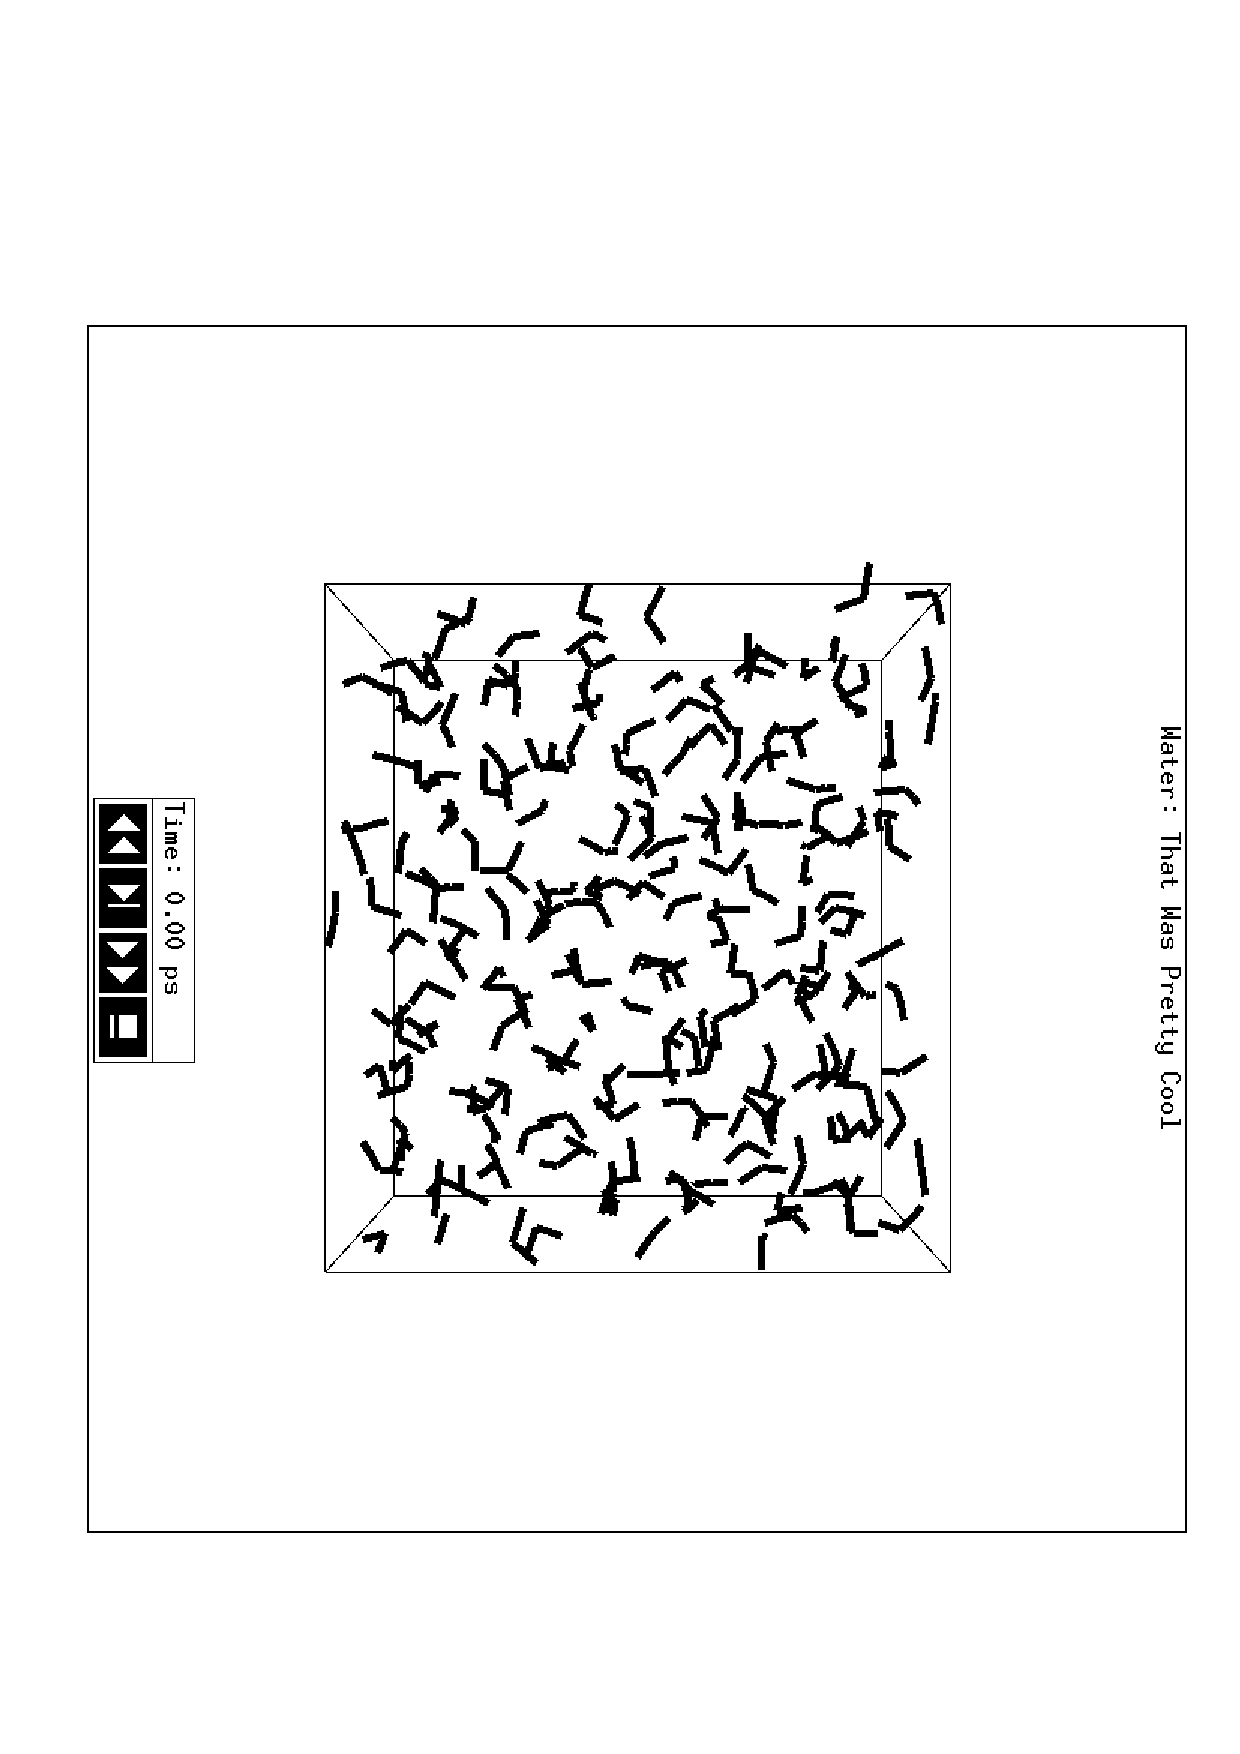
\includegraphics[width=8cm,angle=90]{plots/ngmxdump}}}
\caption{The window of {\tt gmx view} showing a box of water.}
\label{fig:ngmxdump}
\end{figure}
{\tt gmx view}\\
Before analyzing your trajectory it is often informative to look at
your trajectory first. {\gromacs} comes with a simple trajectory
viewer {\tt \normindex{gmx view}}; the advantage with this one is that it does not
require OpenGL, which usually isn't present on {\eg} supercomputers.
It is also possible to generate a
hard-copy in Encapsulated Postscript format (see
\figref{ngmxdump}). If you want a faster and more fancy viewer
 there are several programs
that can read the {\gromacs} trajectory formats -- have a look at our
homepage ({\wwwpage}) for updated links. 

%%%%%%%%%%%%%%%%%%%%%%%%%%%%%%%%%%%%%%% General properties

\section{General properties}
\label{sec:genprop}
{\tt gmx energy, gmx traj}\\
To analyze some or all {\em energies} and other properties, such as
{\em total pressure}, {\em pressure tensor}, {\em density}, {\em
box-volume} and {\em box-sizes}, use the program {\tt \normindex{gmx energy}}.  A
choice can be made from a list a set of energies, like potential,
kinetic or total energy, or individual contributions, like
Lennard-Jones or dihedral energies.

The {\em center-of-mass velocity}, defined as
\beq
{\bf v}_{com} = {1 \over M} \sum_{i=1}^N m_i {\bf v}_i
\eeq
with $M = \sum_{i=1}^N m_i$ the total mass of the system, can be
monitored in time by the program {\tt \normindex{gmx traj} -com -ov}. It is however
recommended to remove the center-of-mass velocity every step (see
\chref{algorithms})!

%%%%%%%%%%%%%%%%%%%%%%%%%%%%%%%%%%%%%%% Radial distribution functions 

\section{Radial distribution functions}
\label{sec:rdf}
{\tt gmx rdf}\\
The {\em radial distribution function} (RDF) or pair correlation
function $g_{AB}(r)$ between particles of type $A$ and $B$ is defined
in the following way:
\newcommand{\dfrac}[2]{\displaystyle \frac{#1}{#2}}
\beq
\begin{array}{rcl}
g_{AB}(r)&=&    \dfrac{\langle \rho_B(r) \rangle}{\langle\rho_B\rangle_{local}}         \\
         &=&    \dfrac{1}{\langle\rho_B\rangle_{local}}\dfrac{1}{N_A}
                \sum_{i \in A}^{N_A} \sum_{j \in B}^{N_B} 
                \dfrac{\delta( r_{ij} - r )}{4 \pi r^2}         \\
\end{array}
\eeq
with $\langle\rho_B(r)\rangle$ the particle density of type $B$ at a distance $r$
around particles $A$, and $\langle\rho_B\rangle_{local}$ the particle density of
type $B$ averaged over all spheres around particles $A$ with radius
$r_{max}$ (see \figref{rdfex}C).

\begin{figure}
\centerline{
{\includegraphics[width=7cm]{plots/rdf}}}
\caption[Definition of slices in {\tt gmx rdf}.]{Definition of slices
in {\tt gmx rdf}: A. $g_{AB}(r)$. B. $g_{AB}(r,\theta)$. The slices are
colored gray. C. Normalization $\langle\rho_B\rangle_{local}$. D. Normalization
$\langle\rho_B\rangle_{local,\:\theta }$. Normalization volumes are colored gray.}
\label{fig:rdfex}
\end{figure}

Usually the value of $r_{max}$ is half of the box length.  The
averaging is also performed in time.  In practice the analysis program
{\tt \normindex{gmx rdf}} divides the system into spherical slices (from $r$ to
$r+dr$, see \figref{rdfex}A) and makes a histogram in stead of
the $\delta$-function. An example of the RDF of oxygen-oxygen in
SPC water~\cite{Berendsen81} is given in \figref{rdf}.

\begin{figure}
\centerline{
{\includegraphics[width=8cm]{plots/rdfO-O}}}
\caption{$g_{OO}(r)$ for Oxygen-Oxygen of SPC-water.}
\label{fig:rdf}
\end{figure}

% TODO: This functionality isn't there...
With {\tt gmx rdf} it is also possible to calculate an angle dependent rdf
$g_{AB}(r,\theta)$, where the angle $\theta$ is defined with respect to a 
certain laboratory axis ${\bf e}$, see \figref{rdfex}B.
\bea 
g_{AB}(r,\theta) &=& {1 \over \langle\rho_B\rangle_{local,\:\theta }} {1 \over N_A} \sum_{i \in A}^{N_A} \sum_{j \in B}^{N_B} {\delta( r_{ij} - r ) \delta(\theta_{ij} -\theta) \over 2 \pi r^2 sin(\theta)}\\
cos(\theta_{ij}) &=& {{\bf r}_{ij} \cdot {\bf e} \over \|r_{ij}\| \;\| e\| }
\eea
This $g_{AB}(r,\theta)$ is useful for analyzing anisotropic systems. 
{\bf Note} that in this case the normalization $\langle\rho_B\rangle_{local,\:\theta}$ is 
the average density in all angle slices from $\theta$ to $\theta + d\theta$ 
up to $r_{max}$, so angle dependent, see \figref{rdfex}D.

%%%%%%%%%%%%%%%%%%%%%%%%%%%%%%%%%%%%%%% Correlation functions 
%\ifthenelse{\equal{\gmxlite}{1}}{}{

\section{Correlation functions}
\label{sec:corr}

\subsection{Theory of correlation functions}
The theory of correlation functions is well established~\cite{Allen87}.
We describe here the implementation of the various 
\normindex{correlation} function flavors in the {\gromacs} code.
The definition of the autocorrelation function\index{autocorrelation function} 
(ACF)
$C_f(t)$ for a property $f(t)$ is:
\beq
C_f(t)  ~=~     \left\langle f(\xi) f(\xi+t)\right\rangle_{\xi}
\label{eqn:corr}
\eeq
where the notation on the right hand side indicates averaging over $\xi$, {\ie} over
time origins.
It is also possible to compute cross-correlation function from two properties
$f(t)$ and $g(t)$:
\beq
C_{fg}(t) ~=~   \left\langle f(\xi) g(\xi+t)\right\rangle_{\xi}
\eeq
however, in {\gromacs} there is no standard mechanism to do this
({\bf note:} you can use the {\tt \normindex{xmgr}} program to compute cross correlations).
The integral of the correlation function over time is the 
correlation time $\tau_f$:
\beq
\tau_f  ~=~     \int_0^{\infty} C_f(t) {\rm d} t
\label{eqn:corrtime}
\eeq

In practice, correlation functions are calculated based on data points with
discrete time intervals {$\Delta$t}, so that the ACF from an MD simulation is:
\beq
C_f(j\Delta t)  ~=~     \frac{1}{N-j}\sum_{i=0}^{N-1-j} f(i\Delta t) f((i+j)\Delta t)
\label{eqn:corrmd}
\eeq
where $N$ is the number of available time frames for the calculation.
The resulting ACF is
obviously only available at time points with the same interval {$\Delta$t}.
Since, for many applications, it is necessary to know the short time behavior
of the ACF ({\eg} the first 10 ps) this often means that we have to save the
data with intervals much shorter than the time scale of interest.
Another implication of \eqnref{corrmd} is that in principle we can not compute
all points of the ACF with the same accuracy, since we have $N-1$ data points
for $C_f(\Delta t)$ but only 1 for $C_f((N-1)\Delta t)$. However, if we decide to
compute only an ACF of length $M\Delta t$, where $M \leq N/2$ we can compute 
all points with the same statistical accuracy:
\beq
C_f(j\Delta t)  ~=~ \frac{1}{M}\sum_{i=0}^{N-1-M} f(i\Delta t)f((i+j)\Delta t)
\eeq
Here of course $j < M$.
$M$ is sometimes referred to as the \normindex{time lag} of the correlation function. 
When we decide to do this, we intentionally do not use all the available points
for very short time intervals ($j << M$), but it makes it easier to interpret
the results.
Another aspect that may not be neglected when computing
ACFs from simulation is that usually the time origins $\xi$ (\eqnref{corr})
are not statistically independent, which may introduce a bias in the results.
This can be tested using a block-averaging procedure, where only time origins
with a spacing at least the length of the time lag are included, {\eg} using 
$k$ time origins with spacing of $M\Delta t$ (where $kM \leq N$):
\beq
C_f(j\Delta t)  ~=~ \frac{1}{k}\sum_{i=0}^{k-1} f(iM\Delta t)f((iM+j)\Delta t)
\eeq
However, one
needs very long simulations to get good accuracy this way, because there are 
many fewer points that contribute to the ACF.

\subsection{Using FFT for computation of the ACF}
The computational cost for calculating an ACF according to \eqnref{corrmd}
is proportional to $N^2$, which is considerable. However, this can be improved
by using fast Fourier transforms to do the convolution~\cite{Allen87}.

\subsection{Special forms of the ACF}
There are some important varieties on the ACF, {\eg} the ACF of a vector \ve{p}:
\beq
C_{\ve{p}}(t) ~=~       \int_0^{\infty} P_n(\cos\angle\left(\ve{p}(\xi),\ve{p}(\xi+t)\right) {\rm d} \xi
\label{eqn:corrleg}
\eeq
where $P_n(x)$ is the $n^{th}$ order Legendre polynomial
\footnote{$P_0(x) = 1$, $P_1(x) = x$, $P_2(x) = (3x^2-1)/2$}.
Such correlation times 
can actually be obtained experimentally using {\eg} NMR or other relaxation 
experiments. {\gromacs} can compute correlations using 
the 1$^{st}$ and 2$^{nd}$ order Legendre polynomial (\eqnref{corrleg}).
This can also be used for rotational autocorrelation
({\tt \normindex{gmx rotacf}})
and dipole autocorrelation ({\tt \normindex{gmx dipoles}}).

In order to study torsion angle dynamics, we define a dihedral 
autocorrelation function as~\cite{Spoel97a}:
\beq
C(t)    ~=~     \left\langle \cos(\theta(\tau)-\theta(\tau+t))\right\rangle_{\tau}
\label{eqn:coenk}
\eeq
{\bf Note} that this is not a  product of two functions 
as is generally used for correlation
functions, but it may be rewritten as the sum of two products:
\beq
C(t)    ~=~     \left\langle\cos(\theta(\tau))\cos(\theta(\tau+t))\,+\,\sin(\theta(\tau))\sin(\theta(\tau+t))\right\rangle_{\tau}
\label{eqn:cot}
\eeq

\subsection{Some Applications}
The program {\tt \normindex{gmx velacc}} calculates the {\em velocity autocorrelation 
function}.
\beq
C_{\ve{v}} (\tau) ~=~ \langle {\ve{v}}_i(\tau) \cdot {\ve{v}}_i(0) \rangle_{i \in A}
\eeq
The self diffusion coefficient can be calculated using the Green-Kubo 
relation~\cite{Allen87}:
\beq
D_A ~=~ {1\over 3} \int_0^{\infty} \langle {\bf v}_i(t) \cdot {\bf v}_i(0) \rangle_{i \in A} \; dt
\eeq
which is just the integral of the velocity autocorrelation function.
There is a widely-held belief that the velocity ACF converges faster than the mean
square displacement (\secref{msd}), which can also be used for the computation of 
diffusion constants. However, Allen \& Tildesley~\cite{Allen87} 
warn us that the long-time 
contribution to the velocity ACF can not be ignored, so care must be taken.

Another important quantity is the dipole correlation time. The {\em dipole 
correlation function} for particles of type $A$ is calculated as follows by 
{\tt \normindex{gmx dipoles}}:
\beq
C_{\mu} (\tau) ~=~
\langle {\bf \mu}_i(\tau) \cdot {\bf \mu}_i(0) \rangle_{i \in A}
\eeq
with ${\bf \mu}_i = \sum_{j \in i} {\bf r}_j q_j$. The dipole correlation time 
can be computed using \eqnref{corrtime}.
For some applications see~\cite{Spoel98a}.

The \normindex{viscosity} of a liquid can be related to the correlation 
time of the Pressure tensor $\ve{P}$~\cite{PSmith93c,Balasubramanian96}.
{\tt \normindex{gmx energy}} can compute the viscosity,
but this is not very accurate~\cite{Hess2002a}, and 
actually the values do not converge.
%} % Brace matches ifthenelse test for gmxlite

\section{Curve fitting in \gromacs}
\subsection{Sum of exponential functions}
Sometimes it is useful to fit a curve to an analytical function, for
example in the case of autocorrelation functions with noisy
tails. {\gromacs} is not a general purpose curve-fitting tool however
and therefore {\gromacs} only supports a limited number of
functions. 
Table~\ref{tab:fitfn} lists the available options with the
corresponding command-line options. The underlying routines for
fitting use the Levenberg-Marquardt algorithm as implemented in the
{\tt lmfit} package~\cite{lmfit} (a bare-bones version of which is
included in {\gromacs} in which an option for error-weighted fitting
was implemented). 
\begin{table}[ht]
\centering
\caption{Overview of fitting functions supported in (most) analysis tools
  that compute autocorrelation functions. The ``Note'' column describes
  properties of the output parameters.}
\label{tab:fitfn}
\begin{tabular}{lcc}
\hline
Command & Functional form $f(t)$& Note\\
line option         &           & \\
\hline
exp        & $e^{-t/{a_0}}$ &\\
aexp      & $a_1e^{-t/{a_0}}$ &\\
exp_exp & $a_1e^{-t/{a_0}}+(1-a_1)e^{-t/{a_2}}$ & $a_2\ge a_0\ge 0$\\
exp5      & $a_1e^{-t/{a_0}}+a_3e^{-t/{a_2}}+a_4$ &$a_2\ge a_0\ge 0$\\
exp7     &
$a_1e^{-t/{a_0}}+a_3e^{-t/{a_2}}+a_5e^{-t/{a_4}}+a_6$&$a_4\ge a_2\ge
a_0 \ge0$\\
exp9    &
$a_1e^{-t/{a_0}}+a_3e^{-t/{a_2}}+a_5e^{-t/{a_4}}+a_7e^{-t/{a_6}}+a_8$&$a_6\ge
a_4\ge a_2\ge a_0\ge 0$\\
\hline
\end{tabular}
\end{table}

\subsection{Error estimation}
Under the hood {\gromacs} implements some more fitting functions,
namely a function to estimate the error in time-correlated data due to Hess~\cite{Hess2002a}:
\beq
\varepsilon^2(t) =
\alpha\tau_1\left(1+\frac{\tau_1}{t}\left(e^{-t/\tau_1}-1\right)\right)
      + (1-\alpha)\tau_2\left(1+\frac{\tau_2}{t}\left(e^{-t/\tau_2}-1\right)\right)
\eeq
where $\tau_1$ and
$\tau_2$ are time constants (with $\tau_2 \ge \tau_1$) and $\alpha$
usually is close to 1 (in the fitting procedure it is enforced that
$0\leq\alpha\leq 1$). This is used in {\tt gmx analyze} for error
estimation using
\beq
\lim_{t\rightarrow\infty}\varepsilon(t) = \sigma\sqrt{\frac{2(\alpha\tau_1+(1-\alpha)\tau_2)}{T}}
\eeq
where $\sigma$ is the standard deviation of the data set and $T$ is
the total simulation time~\cite{Hess2002a}.

\subsection{Interphase boundary demarcation}
In order to determine the position and width of an interface,
Steen-S{\ae}thre {\em et al.} fitted a density profile to the
following function
\beq
f(x) ~=~ \frac{a_0+a_1}{2} - \frac{a_0-a_1}{2}{\rm
  erf}\left(\frac{x-a_2}{a_3^2}\right)
\eeq
where $a_0$ and $a_1$ are densities of different phases, $x$ is the
coordinate normal to the interface, $a_2$ is the position of the
interface and $a_3$ is the width of the
interface~\cite{Steen-Saethre2014a}.
This is implemented in {\tt gmx densorder}.

\subsection{Transverse current autocorrelation function}
In order to establish the transverse current autocorrelation function
(useful for computing viscosity~\cite{Palmer1994a})
the following function is fitted:
\beq
f(x) ~=~ e^{-\nu}\left({\rm cosh}(\omega\nu)+\frac{{\rm
    sinh}(\omega\nu)}{\omega}\right)
\eeq
with $\nu = x/(2a_0)$ and $\omega = \sqrt{1-a_1}$.
This is implemented in {\tt gmx tcaf}.

\subsection{Viscosity estimation from pressure autocorrelation
  function}
The viscosity is a notoriously difficult property to extract from
simulations~\cite{Hess2002a,Wensink2003a}. It is {\em in principle}
possible to determine it by integrating the pressure autocorrelation
function~\cite{PSmith93c}, however this is often hampered by the noisy
tail of the ACF. A workaround to this is fitting the ACF to the
following function~\cite{Guo2002b}:
\beq
f(t)/f(0) = (1-C) {\rm cos}(\omega t) e^{-(t/\tau_f)^{\beta_f}} + C
e^{-(t/\tau_s)^{\beta_s}}
\eeq
where $\omega$ is the frequency of rapid pressure oscillations (mainly
due to bonded forces in molecular simulations), $\tau_f$ and $\beta_f$
are the time constant and exponent of fast relaxation in a
stretched-exponential approximation, $\tau_s$ and $\beta_s$ are constants
for slow relaxation and $C$ is the pre-factor that determines the
weight between fast and slow relaxation. After a fit, the integral of
the function $f(t)$ is used to compute the viscosity:
\beq
\eta = \frac{V}{k_B T}\int_0^{\infty} f(t) dt
\eeq
This equation has been
applied to computing the bulk and shear viscosity using different
elements from the pressure tensor~\cite{Fanourgakis2012a}.
This is implemented in {\tt gmx viscosity}.

\section{Mean Square Displacement}
\label{sec:msd}
{\tt gmx msd}\\
To determine the self diffusion coefficient\index{diffusion coefficient} $D_A$ 
of
particles of type $A$, one can use the \normindex{Einstein
relation}~\cite{Allen87}:
\beq 
\lim_{t \rightarrow \infty} \langle
\|{\bf r}_i(t) - {\bf r}_i(0)\|^2 \rangle_{i \in A} ~=~ 6 D_A t 
\eeq
This {\em mean square displacement} and $D_A$ are calculated by the
program {\tt \normindex{gmx msd}}. Normally an index file containing
atom numbers is used and the MSD is averaged over these atoms.  For
molecules consisting of more than one atom, ${\bf r}_i$ can be taken
as the center of mass positions of the molecules. In that case, you
should use an index file with molecule numbers. The results will be
nearly identical to averaging over atoms, however. The {\tt gmx msd}
program can
also be used for calculating diffusion in one or two dimensions. This
is useful for studying lateral diffusion on interfaces.

An example of the mean square displacement of SPC water is given in
\figref{msdwater}.

\begin{figure}
\centerline{
{\includegraphics[width=8cm]{plots/msdwater}}}
\caption{Mean Square Displacement of SPC-water.}
\label{fig:msdwater}
\end{figure}

%\ifthenelse{\equal{\gmxlite}{1}}{}{
% 
%%%%%%%%%%%%%%%%%%%%% Bonds, angles and dihedral %%%%%%%%%%%%%%%%%%%
% 
\section{Bonds/distances, angles and dihedrals}
\label{sec:bad}
{\tt gmx distance, gmx angle, gmx gangle}\\
To monitor specific {\em bonds} in your modules, or more generally
distances between points, the program
{\tt \normindex{gmx distance}} can calculate distances as a function of
time, as well as the distribution of the distance.
With a traditional index file, the groups should consist of pairs of
atom numbers, for example:
\begin{verbatim}
[ bonds_1 ]
 1     2
 3     4
 9    10

[ bonds_2 ]
12    13
\end{verbatim}
Selections are also supported, with first two positions defining the
first distance, second pair of positions defining the second distance
and so on.  You can calculate the distances between CA and CB atoms in
all your residues (assuming that every residue either has both atoms, or
neither) using a selection such as:
\begin{verbatim}
name CA CB
\end{verbatim}
The selections also allow more generic distances to be computed.
For example, to compute the distances between centers of mass of two
residues, you can use:
\begin{verbatim}
com of resname AAA plus com of resname BBB
\end{verbatim}

The program {\tt \normindex{gmx angle}} calculates the distribution of {\em angles} and
{\em dihedrals} in time. It also gives the average angle or dihedral. 
The index file consists of triplets or quadruples of atom numbers:

\begin{verbatim}
[ angles ]
 1     2     3
 2     3     4
 3     4     5

[ dihedrals ]
 1     2     3     4
 2     3     5     5
\end{verbatim}

For the dihedral angles you can use either the ``biochemical convention'' 
($\phi = 0 \equiv cis$) or ``polymer convention'' ($\phi = 0 \equiv trans$), 
see \figref{dih_def}.

\begin{figure}
\centerline{
{\includegraphics[width=3.5cm,angle=270]{plots/dih-def}}}
\caption[Dihedral conventions.]{Dihedral conventions: A. ``Biochemical
convention''. B. ``Polymer convention''.}
\label{fig:dih_def}
\end{figure}

The program {\tt \normindex{gmx gangle}} provides a selection-enabled
version to compute angles.  This tool can also compute angles and
dihedrals, but does not support all the options of {\tt gmx angle}, such
as autocorrelation or other time series analyses.
In addition, it supports angles between two vectors, a vector and a
plane, two planes (defined by 2 or 3 points, respectively), a
vector/plane and the $z$ axis, or a vector/plane and the normal of a
sphere (determined by a single position).
Also the angle between a vector/plane compared to its position in the
first frame is supported.
For planes, {\tt \normindex{gmx gangle}} uses the normal vector
perpendicular to the plane.
See \figref{sgangle}A, B, C) for the definitions.

\begin{figure}
\centerline{
{\includegraphics{plots/sgangle}}}
\caption[Angle options of {\tt gmx gangle}.]{Angle options of {\tt gmx gangle}:
A. Angle between two vectors.
B. Angle between two planes.
C. Angle between a vector and the $z$ axis.
D. Angle between a vector and the normal of a sphere.
Also other combinations are supported: planes and vectors can be used
interchangeably.}
\label{fig:sgangle}
\end{figure}
%} % Brace matches ifthenelse test for gmxlite

%%%%%%%%%%%%%%%%%%%%%%%%%%%%%%%%%%%%%%% Radius of gyration and distances

\section{Radius of gyration and distances}
\label{sec:rg}
{\tt gmx gyrate, gmx distance, gmx mindist, gmx mdmat, gmx pairdist, gmx xpm2ps}\\
To have a rough measure for the compactness of a structure, you can calculate 
the {\em radius of gyration} with the program {\tt \normindex{gmx gyrate}} as follows:
\beq
R_g ~=~ \left({\frac{\sum_i \|{\bf r}_i\|^2 m_i}{\sum_i m_i}}\right)^{\half}
\label{eqn:rg}
\eeq
where $m_i$ is the mass of atom $i$ and ${\bf r}_i$ the position of 
atom $i$ with respect to the center of mass of the molecule. It is especially 
useful to characterize polymer solutions and proteins. The program will also
provide the radius of gyration around the coordinate axis (or, optionally, principal axes)
by only summing the radii components orthogonal to each axis, for instance
\beq
R_{g,x} ~=~ \left({\frac{\sum_i \left( r_{i,y}^2 + r_{i,z}^2 \right) m_i}{\sum_i m_i}}\right)^{\half}
\label{eqn:rgaxis}
\eeq

Sometimes it is interesting to plot the {\em distance} between two atoms,
or the {\em minimum} distance between two groups of atoms
({\eg}: protein side-chains in a salt bridge). 
To calculate these distances between certain groups there are several 
possibilities:
\begin{description}
\item[$\bullet$] 
The {\em distance between the geometrical centers} of two groups can be 
calculated with the program
%\ifthenelse{\equal{\gmxlite}{1}}{
{{\tt \normindex{gmx distance}}, as explained in \secref{bad}.}
\item[$\bullet$]
The {\em minimum distance} between two groups of atoms during time 
can be calculated with the program {\tt \normindex{gmx mindist}}. It also calculates the 
{\em number of contacts} between these groups 
within a certain radius $r_{max}$.
\item[$\bullet$]
{\tt \normindex{gmx pairdist}} is a selection-enabled version of
{\tt gmx mindist}.
\item[$\bullet$]
To monitor the {\em minimum distances between amino acid residues} 
within a (protein) molecule, you can use 
the program {\tt \normindex{gmx mdmat}}. This minimum distance between two residues
A$_i$ and A$_j$ is defined as the smallest distance between any pair of 
atoms (i $\in$ A$_i$, j $\in$ A$_j$).
The output is a symmetrical matrix of smallest distances 
between all residues.
To visualize this matrix, you can use a program such as {\tt xv}.
If you want to view the axes and legend or if you want to print
the matrix, you can convert it with 
{\tt xpm2ps} into a Postscript picture, see \figref{mdmat}.
\begin{figure}
\centerline{
\includegraphics[width=6.5cm]{plots/distm}}
\caption{A minimum distance matrix for a peptide~\protect\cite{Spoel96b}.}
\label{fig:mdmat}
\end{figure}

Plotting these matrices for different time-frames, one can analyze changes 
in the structure, and {\eg} forming of salt bridges.
\end{description}

%%%%%%%%%%%%%%%%%%%%%%%%%%%%%%%%%%%%%%% Root mean square deviations 

\section{Root mean square deviations in structure}
\label{sec:rmsd}
{\tt gmx rms, gmx rmsdist}\\
The {\em root mean square deviation} ($RMSD$) of certain atoms in a molecule
with respect to a reference structure can be calculated with the program 
{\tt \normindex{gmx rms}} by least-square fitting the structure to the reference structure
($t_2 = 0$) and subsequently calculating the $RMSD$ (\eqnref{rmsd}).
\beq
RMSD(t_1,t_2) ~=~ \left[\frac{1}{M} \sum_{i=1}^N m_i \|{\bf r}_i(t_1)-{\bf r}_i(t_2)\|^2 \right]^{\frac{1}{2}}
\label{eqn:rmsd}
\eeq
where $M = \sum_{i=1}^N m_i$ and ${\bf r}_i(t)$ is the position of atom $i$ at time $t$.
{\bf Note} that fitting does not have to use the same atoms as the calculation
of the $RMSD$; {\eg} a protein is usually fitted on the backbone atoms
(N,C$_{\alpha}$,C), but the $RMSD$ can be computed of the backbone
or of the whole protein.

Instead of comparing the structures to the initial structure at time $t=0$ 
(so for example a crystal structure), one can also calculate \eqnref{rmsd} 
with a structure at time $t_2=t_1-\tau$.
This gives some insight in the mobility as a function of $\tau$.
A matrix can also be made with the $RMSD$ as a function of $t_1$ and $t_2$,
which gives a nice graphical interpretation of a trajectory.
If there are transitions in a trajectory, they will clearly show up in
such a matrix.

Alternatively the $RMSD$ can be computed using a fit-free method with the 
program {\tt \normindex{gmx rmsdist}}:
\beq
RMSD(t) ~=~     \left[\frac{1}{N^2}\sum_{i=1}^N \sum_{j=1}^N    \|{\bf r}_{ij}(t)-{\bf r}_{ij}(0)\|^2\right]^{\frac{1}{2}}
\label{eqn:rmsdff}
\eeq
where the {\em distance} {\bf r}$_{ij}$ between atoms at time $t$ 
is compared with the distance between the same atoms at time $0$.

%\ifthenelse{\equal{\gmxlite}{1}}{}{
\section{Covariance analysis\index{covariance analysis}}
\label{sec:covanal}
Covariance analysis, also called
\seeindex{principal component analysis}{covariance analysis}
or \seeindex{essential dynamics}{covariance analysis}
\cite{Amadei93}{,} can find correlated motions.
It uses the covariance matrix $C$ of the atomic coordinates:
\beq
C_{ij} = \left \langle 
M_{ii}^{\frac{1}{2}} (x_i - \langle x_i \rangle)
M_{jj}^{\frac{1}{2}}  (x_j - \langle x_j \rangle)
\right \rangle
\eeq
where $M$ is a diagonal matrix containing the masses of the atoms
(mass-weighted analysis) or the unit matrix (non-mass weighted analysis).
$C$ is a symmetric $3N \times 3N$ matrix, which can be diagonalized with
an orthonormal transformation matrix $R$:
\beq
R^T C R = \mbox{diag}(\lambda_1,\lambda_2,\ldots,\lambda_{3N})
~~~~\mbox{where}~~\lambda_1 \geq \lambda_2 \geq \ldots \geq \lambda_{3N}
\eeq
The columns of $R$ are the eigenvectors, also called principal or
essential modes.
$R$ defines a transformation to a new coordinate system. The trajectory
can be projected on the principal modes to give the principal components
$p_i(t)$:
\beq
{\bf p}(t) = R^T M^{\frac{1}{2}} ({\bf x}(t) - \langle {\bf x} \rangle)
\eeq
The eigenvalue $\lambda_i$ is the mean square fluctuation of principal
component $i$. The first few principal modes often describe 
collective, global motions in the system.
The trajectory can be filtered along one (or more) principal modes.
For one principal mode $i$ this goes as follows:
\beq
{\bf x}^f(t) =
\langle {\bf x} \rangle + M^{-\frac{1}{2}} R_{*i} \, p_i(t)
\eeq

When the analysis is performed on a macromolecule, one often wants to
remove the overall rotation and translation to look at the internal motion
only. This can be achieved by least square fitting to a reference structure.
Care has to be taken that the reference structure is representative for the
ensemble, since the choice of reference structure influences the covariance
matrix.

One should always check if the principal modes are well defined.
If the first principal component resembles a half cosine and
the second resembles a full cosine, you might be filtering noise (see below).
A good way to check the relevance of the first few principal
modes is to calculate the overlap of the sampling between
the first and second half of the simulation.
{\bf Note} that this can only be done when the same reference structure is
used for the two halves.

A good measure for the overlap has been defined in~\cite{Hess2002b}.
The elements of the covariance matrix are proportional to the square
of the displacement, so we need to take the square root of the matrix
to examine the extent of sampling. The square root can be
calculated from the eigenvalues $\lambda_i$ and the eigenvectors,
which are the columns of the rotation matrix $R$.
For a symmetric and diagonally-dominant matrix $A$ of size $3N \times 3N$
the square root can be calculated as:
\beq
A^\frac{1}{2} = 
R \, \mbox{diag}(\lambda_1^\frac{1}{2},\lambda_2^\frac{1}{2},\ldots,\lambda_{3N}^\frac{1}{2}) \, R^T
\eeq
It can be verified easily that the product of this matrix with itself gives
$A$.
Now we can define a difference $d$ between covariance matrices $A$ and $B$
as follows:
\begin{eqnarray}
d(A,B) & = & \sqrt{\mbox{tr}\left(\left(A^\frac{1}{2} - B^\frac{1}{2}\right)^2\right)
}
\\ & = &
\sqrt{\mbox{tr}\left(A + B - 2 A^\frac{1}{2} B^\frac{1}{2}\right)}
\\ & = &
\left( \sum_{i=1}^N \left( \lambda_i^A + \lambda_i^B \right)
- 2 \sum_{i=1}^N \sum_{j=1}^N \sqrt{\lambda_i^A \lambda_j^B}
\left(R_i^A \cdot R_j^B\right)^2 \right)^\frac{1}{2}
\end{eqnarray}
where tr is the trace of a matrix.
We can now define the overlap $s$ as:
\beq
s(A,B) = 1 - \frac{d(A,B)}{\sqrt{\mbox{tr}A + \mbox{tr} B}}
\eeq
The overlap is 1 if and only if matrices $A$ and $B$ are identical.
It is 0 when the sampled subspaces are completely orthogonal.

A commonly-used measure is the subspace overlap of the first few
eigenvectors of covariance matrices.
The overlap of the subspace spanned by $m$ orthonormal vectors 
${\bf w}_1,\ldots,{\bf w}_m$ with a reference subspace spanned by 
$n$ orthonormal vectors ${\bf v}_1,\ldots,{\bf v}_n$
can be quantified as follows:
\beq
\mbox{overlap}({\bf v},{\bf w}) =
\frac{1}{n} \sum_{i=1}^n \sum_{j=1}^m ({\bf v}_i \cdot {\bf w}_j)^2
\eeq
The overlap will increase with increasing $m$ and will be 1 when
set ${\bf v}$ is a subspace of set ${\bf w}$.
The disadvantage of this method is that it does not take the eigenvalues
into account. All eigenvectors are weighted equally, and when
degenerate subspaces are present (equal eigenvalues), the calculated overlap
will be too low.

Another useful check is the cosine content. It has been proven that the
the principal components of random diffusion are cosines with the number of
periods equal to half the principal component index~\cite{Hess2000,Hess2002b}.
The eigenvalues are proportional to the index to the power $-2$.
The cosine content is defined as:
\beq
\frac{2}{T}
\left( \int_0^T \cos\left(\frac{i \pi t}{T}\right) \, p_i(t) \mbox{d} t \right)^2
\left( \int_0^T p_i^2(t) \mbox{d} t \right)^{-1}
\eeq
When the cosine content of the first few principal components
is close to 1, the largest fluctuations are not connected with
the potential, but with random diffusion.

The covariance matrix is built and diagonalized by
{\tt \normindex{gmx covar}}.
The principal components and overlap (and many more things)
can be plotted and analyzed with {\tt \normindex{gmx anaeig}}.
The cosine content can be calculated with {\tt \normindex{gmx analyze}}.
%} % Brace matches ifthenelse test for gmxlite

%\ifthenelse{\equal{\gmxlite}{1}}{}{
\section{Dihedral principal component analysis}
{\tt gmx angle, gmx covar, gmx anaeig}\\
Principal component analysis can be performed in dihedral
space~\cite{Mu2005a} using {\gromacs}. You start by defining the
dihedral angles of interest in an index file, either using {\tt
 gmx mk_angndx} or otherwise. Then you use the {\tt gmx angle} program
with the {\tt -or} flag to produce a new {\tt .trr} file containing the cosine and
sine of each dihedral angle in two coordinates, respectively. That is,
in the {\tt .trr} file you will have a series of numbers corresponding to:
cos($\phi_1$), sin($\phi_1$), cos($\phi_2$), sin($\phi_2$), ...,
cos($\phi_n$), sin($\phi_n$), and the array is padded with zeros, if
necessary.  Then you can use this {\tt .trr} file as input for the {\tt
 gmx covar} program and perform principal component analysis as usual.
For this to work you will need to generate a reference file ({\tt .tpr}, 
{\tt .gro}, {\tt .pdb} etc.) containing the same number of ``atoms'' 
as the new {\tt .trr} file, that is for $n$ dihedrals you need 2$n$/3 atoms 
(rounded up if not an integer number). 
You should use the {\tt -nofit} option for {\tt
gmx covar} since the coordinates in the dummy reference file do not
correspond in any way to the information in the {\tt .trr} file. Analysis of
the results is done using {\tt gmx anaeig}.
%} % Brace matches ifthenelse test for gmxlite
 
%%%%%%%%%%%%%%%%%%%%%%%%%%%%%%%%%%%%%%% Hydrogen bonds

\section{Hydrogen bonds}
{\tt gmx hbond}\\
The program {\tt \normindex{gmx hbond}} analyzes the {\em hydrogen bonds} (H-bonds)
between all possible donors D and acceptors A. To determine if an
H-bond exists, a geometrical criterion is used, see also
\figref{hbond}:
\beq
\begin{array}{rclcl}
r       & \leq  & r_{HB}        & = & 0.35~\mbox{nm}    \\
\alpha  & \leq  & \alpha_{HB}   & = & 30^o              \\
\end{array}
\eeq

\begin{figure}
\centerline{\includegraphics[width=2.5cm,angle=270]{plots/hbond}}
\caption{Geometrical Hydrogen bond criterion.}
\label{fig:hbond}
\end{figure}

The value of $r_{HB} = 0.35$~nm corresponds to the first minimum of the RDF of 
SPC water (see also \figref{rdf}).

The program {\tt gmx hbond} analyzes all hydrogen bonds existing
between two groups of atoms (which must be either identical or
non-overlapping) or in specified donor-hydrogen-acceptor triplets, in
the following ways:

\begin{figure}
\centerline{
{\includegraphics[width=5cm,angle=270]{plots/hbond-insert}}}
\caption[Insertion of water into an H-bond.]{Insertion of water into
an H-bond. (1) Normal H-bond between two residues. (2) H-bonding
bridge via a water molecule.}
\label{fig:insert}
\end{figure}

\begin{itemize}
\item
Donor-Acceptor distance ($r$) distribution of all H-bonds
\item
Hydrogen-Donor-Acceptor angle ($\alpha$) distribution of all H-bonds 
\item
The total number of H-bonds in each time frame
\item
\newcommand{\nn}[1]{$n$-$n$+$#1$}
The number of H-bonds in time between residues, divided into groups
\nn{i} where $n$ and $n$+$i$ stand for residue numbers and $i$ goes
from 0 to 6. The group for $i=6$ also includes all H-bonds for
$i>6$. These groups include the \nn{3}, \nn{4} and \nn{5} H-bonds,
which provide a measure for the formation of $\alpha$-helices or
$\beta$-turns or strands.
\item
The lifetime of the H-bonds is calculated from the average over all
autocorrelation functions of the existence functions (either 0 or 1)
of all H-bonds:
\beq
C(\tau) ~=~ \langle s_i(t)~s_i (t + \tau) \rangle
\label{eqn:hbcorr}
\eeq
with $s_i(t) = \{0,1\}$ for H-bond $i$ at time $t$. The integral of
$C(\tau)$ gives a rough estimate of the average H-bond lifetime
$\tau_{HB}$:
\beq
\tau_{HB} ~=~ \int_{0}^{\infty} C(\tau) d\tau
\label{eqn:hblife}
\eeq
Both the integral and the complete autocorrelation function $C(\tau)$
will be output, so that more sophisticated analysis ({\eg}\@ using
multi-exponential fits) can be used to get better estimates for
$\tau_{HB}$. A more complete analysis is given in ref.~\cite{Spoel2006b};
one of the more fancy option is the Luzar and Chandler analysis
of hydrogen bond kinetics~\cite{Luzar96b,Luzar2000a}. 
\item
An H-bond existence map can be generated of dimensions {\em
\#~H-bonds}$\times${\em \#~frames}. The ordering is identical to the index 
file (see below), but reversed, meaning that the last triplet in the index
file corresponds to the first row of the existence map.
\item
Index groups are output containing the analyzed groups, all
donor-hydrogen atom pairs and acceptor atoms in these groups,
donor-hydrogen-acceptor triplets involved in hydrogen bonds between
the analyzed groups and all solvent atoms involved in insertion.

\end{itemize}

%\ifthenelse{\equal{\gmxlite}{1}}{}{
%
%%%%%%%%%%%%%%%%%%%%%%%%%%%%%%%%%%%%%%% Protein related items 

\section{Protein-related items}
{\tt gmx do_dssp, gmx rama, gmx wheel}\\
To analyze structural changes of a protein, you can calculate the radius of 
gyration or the minimum residue distances over time 
(see \secref{rg}), or calculate the RMSD (\secref{rmsd}).

You can also look at the changing of {\em secondary structure elements} 
during your run. For this, you can use the program {\tt \normindex{gmx do_dssp}}, which is 
an interface for the commercial program {\tt DSSP}~\cite{Kabsch83}. For 
further information, see the {\tt DSSP} manual. A typical output plot of 
{\tt gmx do_dssp} is given in \figref{dssp}.

\begin{figure}
\centerline{
\includegraphics[width=12cm]{plots/dssp}}
\caption{Analysis of the secondary structure elements of a peptide in time.}
\label{fig:dssp}
\end{figure}

One other important analysis of proteins is the so-called 
{\em Ramachandran plot}. 
This is the projection of the structure on the two dihedral angles $\phi$ and 
$\psi$ of the protein backbone, see \figref{phipsi}.

\begin{figure}
\centerline{
\includegraphics[width=5cm]{plots/phipsi}}
\caption{Definition of the dihedral angles $\phi$ and $\psi$ of the protein backbone.}
\label{fig:phipsi}
\end{figure}

To evaluate this Ramachandran plot you can use the program {\tt
\normindex{gmx rama}}.
A typical output is given in \figref{rama}.

\begin{figure}
\centerline{
{\includegraphics[width=8cm]{plots/rama}}}
\caption{Ramachandran plot of a small protein.}
\label{fig:rama}
\end{figure}

When studying $\alpha$-helices 
it is useful to have a {\em helical wheel} projection
of your peptide, to see whether a peptide is amphipathic. This can be done
using the {\tt \normindex{gmx wheel}} program. Two examples are
plotted in \figref{wheel}.

\begin{figure}
\centerline{\includegraphics[width=\htw]{plots/hpr-wheel}}
\caption{Helical wheel projection of the N-terminal helix of HPr.}
\label{fig:wheel}
\end{figure}

%%%%%%%%%%%%%%%%%%%%%%%%%%%%%%%%%%%%%%% Membrane Related Items

\section{Interface-related items}
{\tt gmx order, gmx density, gmx potential, gmx traj}\\
When simulating molecules with long carbon tails, it can be
interesting to calculate their average orientation. There are several
flavors of order parameters, most of which are related. The program
{\tt \normindex{gmx order}} can calculate order parameters using the equation:

\begin{equation}
S_{z} = \frac{3}{2}\langle {\cos^2{\theta_z}} \rangle - \frac{1}{2}
\label{eqn:Sgr}
\end{equation}
where $\theta_z$ is the angle between the $z$-axis of the simulation
box and the molecular axis under consideration. The latter is defined as the
vector from C$_{n-1}$ to C$_{n+1}$. The parameters $S_x$
and $S_y$ are defined in the same way. The brackets imply averaging over time
and molecules. Order parameters can vary between 1 (full order along
the interface normal) and $-1/2$ (full order perpendicular to the
normal), with a value of zero in the case of isotropic orientation.

The program can do two things for you. It can calculate the order
parameter for each CH$_2$ segment separately, for any of three axes,
or it can divide the box in slices and calculate the average value of
the order parameter per segment in one slice. The first method gives
an idea of the ordering of a molecule from head to tail, the second
method gives an idea of the ordering as function of the box length.

The electrostatic potential ($\psi$) across the interface can be
computed from a trajectory by evaluating the double integral of the
charge density ($\rho(z)$):
\beq
\psi(z) - \psi(-\infty) = - \int_{-\infty}^z dz' \int_{-\infty}^{z'} \rho(z'')dz''/ \epsilon_0 
\label{eqn:elpotgr}
\eeq
where the position $z=-\infty$ is far enough in the bulk phase such that
the field is zero.  With this method, it is possible to ``split'' the
total potential into separate contributions from lipid and water
molecules. The program {\tt \normindex{gmx potential}} divides the box in slices and
sums all charges of the atoms in each slice. It then integrates this
charge density to give the electric field, which is in turn integrated to
give the potential. Charge density, electric field, and potential are written
to {\tt xvgr} input files.

The program {\tt \normindex{gmx traj}} is a very simple analysis program. All it
does is print the coordinates, velocities, or forces of selected atoms.
It can also calculate the center of mass of one or more
molecules and print the coordinates of the center of mass to three
files. By itself, this is probably not a very useful analysis, but
having the coordinates of selected molecules or atoms can be very
handy for further analysis, not only in interfacial systems.

The program {\tt \normindex{gmx density}} calculates the mass density of
groups and gives a plot of the density against a box
axis. This is useful for looking at the distribution of groups or
atoms across the interface.

%%%%%%%%%%%%%%%%%%%%%%%%%%%%%%%%%%%%%%% Chemical shifts

% \section{Chemical shifts}
% {\tt total, do_shift}\\
% You can compute the NMR chemical shifts of protons with the program
% {\tt \normindex{do_shift}}. This is just an {\gromacs} interface to
% the public domain program {\tt total}~\cite{Williamson93a}. For
% further information, read the article. Although there is limited
% support for this in {\gromacs}, users are encouraged to use the
% software provided by David Case's group at Scripps because it seems
% to be more up-to-date.

%%%%%%%%%%%%%%%%%%%%%%%%%%%%%%%%%%%%%%%
%} % Brace matches ifthenelse test for gmxlite

% LocalWords:  Xmgr ndx mk angndx rdf dihedrals grompp hydrogens MainChain Prot
% LocalWords:  oxygens SideChain tryptophan vsitetop aminoacids dat ngmx dr SPC
% LocalWords:  OO ACF fg xmgr corrmd ACFs kM iM FFT th NMR nd corrleg rotacf dt
% LocalWords:  velacc Kubo msd Tildesley corrtime msdwater sgangle cis dih xpm
% LocalWords:  mindist mdmat rms rmsdist rmsd jj diag eigenvectors covar anaeig
% LocalWords:  macromolecule trr tpr gro pdb nofit hbond rclcl HB multi Luzar
% LocalWords:  dssp rama xrama rg Ramachandran phipsi amphipathic HPr xvgr pvd
% LocalWords:  Scripps RDF online usinggroups mdrun groupconcept HOH
% LocalWords:  residuetypes determinding OpenGL traj ov rcl ij ps nm
% LocalWords:  autocorrelation interfacial pairdist

\ifthenelse{\equal{\gmxlite}{1}}{}{
%
%       A P P E N D I C E S
%
\appendix
\include{technical}
%
% This file is part of the GROMACS molecular simulation package.
%
% Copyright (c) 2013,2014,2015, by the GROMACS development team, led by
% Mark Abraham, David van der Spoel, Berk Hess, and Erik Lindahl,
% and including many others, as listed in the AUTHORS file in the
% top-level source directory and at http://www.gromacs.org.
%
% GROMACS is free software; you can redistribute it and/or
% modify it under the terms of the GNU Lesser General Public License
% as published by the Free Software Foundation; either version 2.1
% of the License, or (at your option) any later version.
%
% GROMACS is distributed in the hope that it will be useful,
% but WITHOUT ANY WARRANTY; without even the implied warranty of
% MERCHANTABILITY or FITNESS FOR A PARTICULAR PURPOSE.  See the GNU
% Lesser General Public License for more details.
%
% You should have received a copy of the GNU Lesser General Public
% License along with GROMACS; if not, see
% http://www.gnu.org/licenses, or write to the Free Software Foundation,
% Inc., 51 Franklin Street, Fifth Floor, Boston, MA  02110-1301  USA.
%
% If you want to redistribute modifications to GROMACS, please
% consider that scientific software is very special. Version
% control is crucial - bugs must be traceable. We will be happy to
% consider code for inclusion in the official distribution, but
% derived work must not be called official GROMACS. Details are found
% in the README & COPYING files - if they are missing, get the
% official version at http://www.gromacs.org.
%
% To help us fund GROMACS development, we humbly ask that you cite
% the research papers on the package. Check out http://www.gromacs.org.

\chapter{Some implementation details}
In this chapter we will present some implementation details. This is
far from complete, but we deemed it necessary to clarify some things
that would otherwise be hard to understand.

\section{Single Sum Virial in {\gromacs}}
\label{sec:virial}
The \normindex{virial} $\Xi$ can be written in full tensor form as:
\beq
\Xi~=~-\half~\sum_{i < j}^N~\rvij\otimes\Fvij
\eeq
where $\otimes$ denotes the {\em direct product} of two vectors.\footnote
{$({\bf u}\otimes{\bf v})^{\ab}~=~{\bf u}_{\al}{\bf v}_{\be}$} When this is 
computed in the inner loop of an MD program 9 multiplications and 9
additions are needed.\footnote{The calculation of 
Lennard-Jones and Coulomb forces is about 50 floating point operations.}

Here it is shown how it is possible to extract the virial calculation
from the inner loop~\cite{Bekker93b}.

\subsection{Virial}
In a system with periodic boundary conditions\index{periodic boundary 
conditions}, the
periodicity must be taken into account for the virial:
\beq
\Xi~=~-\half~\sum_{i < j}^{N}~\rnij\otimes\Fvij
\eeq
where $\rnij$ denotes the distance vector of the
{\em nearest image} of atom $i$ from atom $j$. In this definition we add
a {\em shift vector} $\delta_i$ to the position vector $\rvi$ 
of atom $i$. The difference vector $\rnij$ is thus equal to:
\beq
\rnij~=~\rvi+\delta_i-\rvj
\eeq
or in shorthand:
\beq
\rnij~=~\rni-\rvj
\eeq
In a triclinic system, there are 27 possible images of $i$; when a truncated 
octahedron is used, there are 15 possible images.

\subsection{Virial from non-bonded forces}
Here the derivation for the single sum virial in the {\em non-bonded force} 
routine is given. $i \neq j$ in all formulae below.
\newcommand{\di}{\delta_{i}}
\newcommand{\qrt}{\frac{1}{4}}
\bea
\Xi	
&~=~&-\half~\sum_{i < j}^{N}~\rnij\otimes\Fvij				\\
&~=~&-\qrt\sum_{i=1}^N~\sum_{j=1}^N ~(\rvi+\di-\rvj)\otimes\Fvij	\\
&~=~&-\qrt\sum_{i=1}^N~\sum_{j=1}^N ~(\rvi+\di)\otimes\Fvij-\rvj\otimes\Fvij	\\
&~=~&-\qrt\left(\sum_{i=1}^N~\sum_{j=1}^N ~(\rvi+\di)\otimes\Fvij~-~\sum_{i=1}^N~\sum_{j=1}^N ~\rvj\otimes\Fvij\right)	\\
&~=~&-\qrt\left(\sum_{i=1}^N~(\rvi+\di)\otimes\sum_{j=1}^N~\Fvij~-~\sum_{j=1}^N ~\rvj\otimes\sum_{i=1}^N~\Fvij\right)	\\
&~=~&-\qrt\left(\sum_{i=1}^N~(\rvi+\di)\otimes\Fvi~+~\sum_{j=1}^N ~\rvj\otimes\Fvj\right)	\\
&~=~&-\qrt\left(2~\sum_{i=1}^N~\rvi\otimes\Fvi+\sum_{i=1}^N~\di\otimes\Fvi\right)
\eea
In these formulae we introduced:
\bea
\Fvi&~=~&\sum_{j=1}^N~\Fvij					\\
\Fvj&~=~&\sum_{i=1}^N~\Fvji
\eea
which is the total force on $i$ with respect to $j$. Because we use Newton's Third Law:
\beq
\Fvij~=~-\Fvji
\eeq
we must, in the implementation, double the term containing the shift $\delta_i$.

\subsection{The intra-molecular shift (mol-shift)}
For the bonded forces and SHAKE it is possible to make a {\em mol-shift}
list, in which the periodicity is stored. We simple have an array {\tt mshift}
in which for each atom an index in the {\tt shiftvec} array is stored.

The algorithm to generate such a list can be derived from graph theory,
considering each particle in a molecule as a bead in a graph, the bonds 
as edges.
\begin{enumerate}
\item[1]	Represent the bonds and atoms as bidirectional graph
\item[2]	Make all atoms white
\item[3]	Make one of the white atoms black (atom $i$) and put it in the
		central box
\item[4]	Make all of the neighbors of $i$ that are currently 
		white, gray 
\item[5]	Pick one of the gray atoms (atom $j$), give it the
		correct periodicity with respect to any of 
		its black neighbors
		and make it black
\item[6]	Make all of the neighbors of $j$ that are currently 
		white, gray
\item[7]	If any gray atom remains, go to [5]
\item[8]	If any white atom remains, go to [3]
\end{enumerate}
Using this algorithm we can 
\begin{itemize}
\item	optimize the bonded force calculation as well as SHAKE 
\item	calculate the virial from the bonded forces
	in the single sum method again
\end{itemize}

Find a representation of the bonds as a bidirectional graph.

\subsection{Virial from Covalent Bonds}
Since the covalent bond force gives a contribution to the virial, we have:
\bea
b	&~=~&	\|\rnij\|					\\
V_b	&~=~&	\half k_b(b-b_0)^2				\\
\Fvi	&~=~&	-\nabla V_b					\\
	&~=~&	k_b(b-b_0)\frac{\rnij}{b}			\\
\Fvj	&~=~&	-\Fvi
\eea
The virial contribution from the bonds then is:
\bea
\Xi_b	&~=~&	-\half(\rni\otimes\Fvi~+~\rvj\otimes\Fvj)	\\
	&~=~&	-\half\rnij\otimes\Fvi
\eea

\subsection{Virial from SHAKE}
An important contribution to the virial comes from shake. Satisfying 
the constraints a force {\bf G} that is exerted on the particles ``shaken.'' If this
force does not come out of the algorithm (as in standard SHAKE) it can be
calculated afterward (when using {\em leap-frog}) by:
\bea
\Delta\rvi&~=~&\rvi(t+\Dt)-
[\rvi(t)+{\bf v}_i(t-\frac{\Dt}{2})\Dt+\frac{\Fvi}{m_i}\Dt^2]	\\
{\bf G}_i&~=~&\frac{m_i\Delta\rvi}{\Dt^2}
\eea
This does not help us in the general case. Only when no periodicity
is needed (like in rigid water) this can be used, otherwise
we must add the virial calculation in the inner loop of SHAKE.

When it {\em is} applicable the virial can be calculated in the single sum way:
\beq
\Xi~=~-\half\sum_i^{N_c}~\rvi\otimes\Fvi
\eeq
where $N_c$ is the number of constrained atoms.

%Another method is the Non-Iterative shake as proposed (and implemented)
%by Yoneya. In this algorithm the Lagrangian multipliers are solved in a 
%matrix equation, and given these multipliers it is easy to get the periodicity
%in the virial afterwards. 

%More...


\section{Optimizations}
Here we describe some of the algorithmic optimizations used 
in {\gromacs}, apart from parallelism. 

\subsection{Inner Loops for Water}
\label{sec:waterloops}
{\gromacs} uses special inner loops to calculate non-bonded
interactions for water molecules with other atoms, and yet
another set of loops for interactions between pairs of
water molecules. There highly optimized loops for two types of water models.
For three site models similar to
SPC~\cite{Berendsen81}, {\ie}:
\begin{enumerate}
\item   There are three atoms in the molecule.
\item   The whole molecule is a single charge group.
\item   The first atom has Lennard-Jones (\secref{lj}) and 
        Coulomb (\secref{coul}) interactions.
\item   Atoms two and three have only Coulomb interactions, 
        and equal charges.
\end{enumerate}
These loops also works for the SPC/E~\cite{Berendsen87} and 
TIP3P~\cite{Jorgensen83} water models.
And for four site water models similar to TIP4P~\cite{Jorgensen83}:
\begin{enumerate}
\item   There are four atoms in the molecule.
\item   The whole molecule is a single charge group.
\item   The first atom has only Lennard-Jones (\secref{lj}) interactions.
\item   Atoms two and three have only Coulomb (\secref{coul}) interactions, 
        and equal charges.
\item   Atom four has only Coulomb interactions.
\end{enumerate}

The benefit of these implementations is that there are more floating-point
operations in a single loop, which implies that some compilers
can schedule the code better. However, it turns out that even
some of the most advanced compilers have problems with scheduling, 
implying that manual tweaking is necessary to get optimum 
\normindex{performance}.
This may include common-sub-expression elimination, or moving
code around. 

% LocalWords:  Virial virial triclinic intra mol mshift shiftvec sqrt SPC lj yf
% LocalWords:  coul

%
% This file is part of the GROMACS molecular simulation package.
%
% Copyright (c) 2013,2014,2017, by the GROMACS development team, led by
% Mark Abraham, David van der Spoel, Berk Hess, and Erik Lindahl,
% and including many others, as listed in the AUTHORS file in the
% top-level source directory and at http://www.gromacs.org.
%
% GROMACS is free software; you can redistribute it and/or
% modify it under the terms of the GNU Lesser General Public License
% as published by the Free Software Foundation; either version 2.1
% of the License, or (at your option) any later version.
%
% GROMACS is distributed in the hope that it will be useful,
% but WITHOUT ANY WARRANTY; without even the implied warranty of
% MERCHANTABILITY or FITNESS FOR A PARTICULAR PURPOSE.  See the GNU
% Lesser General Public License for more details.
%
% You should have received a copy of the GNU Lesser General Public
% License along with GROMACS; if not, see
% http://www.gnu.org/licenses, or write to the Free Software Foundation,
% Inc., 51 Franklin Street, Fifth Floor, Boston, MA  02110-1301  USA.
%
% If you want to redistribute modifications to GROMACS, please
% consider that scientific software is very special. Version
% control is crucial - bugs must be traceable. We will be happy to
% consider code for inclusion in the official distribution, but
% derived work must not be called official GROMACS. Details are found
% in the README & COPYING files - if they are missing, get the
% official version at http://www.gromacs.org.
%
% To help us fund GROMACS development, we humbly ask that you cite
% the research papers on the package. Check out http://www.gromacs.org.

%%%%%%%%%%%%%%%%%%%%%%%%%%%%%%%%%%%%%%%%%%%%%%%%%%%%%%%%%%%%%%%%%%%%%%%%%
%
%       AVERAGES AND FLUCTUATIONS
%
%%%%%%%%%%%%%%%%%%%%%%%%%%%%%%%%%%%%%%%%%%%%%%%%%%%%%%%%%%%%%%%%%%%%%%%%%
\chapter{Averages and fluctuations}
\section{Formulae for averaging}
{\bf Note:} this section was taken from ref~\cite{Gunsteren94a}.

When analyzing a MD trajectory averages $\left<x\right>$ and fluctuations
\beq
 \left<(\Delta x)^2\right>^{\half} ~=~ \left<[x-\left<x\right>]^2\right>^{\half}
\label{eqn:var0}
\eeq
of a quantity $x$ are to be computed.
The variance $\sigma_x$ of a series of N$_x$ values, 
\{x$_i$\}, can be computed from
\beq
\sigma_x~=~ \sum_{i=1}^{N_x} x_i^2 ~-~  \frac{1}{N_x}\left(\sum_{i=1}^{N_x}x_i\right)^2
\label{eqn:var1}
\eeq
Unfortunately this formula is numerically not very accurate, 
especially when $\sigma_x^{\half}$ is small compared to the values of $x_i$. 
The following (equivalent) expression is numerically more accurate
\beq
\sigma_x ~=~ \sum_{i=1}^{N_x} [x_i  - \left<x\right>]^2
\eeq
with
\beq
  \left<x\right> ~=~ \frac{1}{N_x} \sum_{i=1}^{N_x} x_i
\label{eqn:var2}
\eeq
Using ~\eqnsref{var1}{var2} one has to go 
through the series of $x_i$ values twice, once to determine 
$\left<x\right>$ and again to 
compute $\sigma_x$, 
whereas \eqnref{var0} requires only one sequential scan of
the series \{x$_i$\}. However, one may cast \eqnref{var1} in
another form, containing partial sums, which allows for a sequential 
update algorithm. Define the partial sum
\beq
          X_{n,m} ~=~ \sum_{i=n}^{m} x_i                      
\eeq
and the partial variance
\beq
    \sigma_{n,m} ~=~ \sum_{i=n}^{m}  \left[x_i - \frac{X_{n,m}}{m-n+1}\right]^2  
\label{eqn:sigma}
\eeq
It can be shown that
\beq
          X_{n,m+k} ~=~  X_{n,m} + X_{m+1,m+k}         
\label{eqn:Xpartial}
\eeq
and
\bea
\sigma_{n,m+k} &=& \sigma_{n,m} + \sigma_{m+1,m+k} + \left[~\frac {X_{n,m}}{m-n+1} - \frac{X_{n,m+k}}{m+k-n+1}~\right]^2~* \nonumber\\
   && ~\frac{(m-n+1)(m+k-n+1)}{k}
\label{eqn:varpartial}
\eea
For $n=1$ one finds
\beq
\sigma_{1,m+k} ~=~ \sigma_{1,m} + \sigma_{m+1,m+k}~+~
  \left[~\frac{X_{1,m}}{m} - \frac{X_{1,m+k}}{m+k}~\right]^2~ \frac{m(m+k)}{k}
\label{eqn:sig1}
\eeq
and for $n=1$ and $k=1$ ~(\eqnref{varpartial}) becomes
\bea
\sigma_{1,m+1}  &=& \sigma_{1,m} + 
                        \left[\frac{X_{1,m}}{m} - \frac{X_{1,m+1}}{m+1}\right]^2 m(m+1)\\
                &=& \sigma_{1,m} + 
                        \frac {[~X_{1,m} - m x_{m+1}~]^2}{m(m+1)}
\label{eqn:simplevar0}
\eea
where we have used the relation
\beq
     X_{1,m+1} ~=~  X_{1,m} + x_{m+1}                       
\label{eqn:simplevar1}
\eeq
Using formulae~(\eqnref{simplevar0}) and ~(\eqnref{simplevar1}) the average 
\beq
\left<x\right> ~=~ \frac{X_{1,N_x}}{N_x}
\eeq
and the fluctuation 
\beq
\left<(\Delta x)^2\right>^{\half} = \left[\frac {\sigma_{1,N_x}}{N_x}\right]^{\half}
\eeq
can be obtained by one sweep through the data. 

\section{Implementation}
In {\gromacs} the instantaneous
energies $E(m)$ are stored in the \swapindex{energy}{file}, along with the 
values of $\sigma_{1,m}$ and $X_{1,m}$. Although the steps are counted from 0,
for the energy and fluctuations steps are counted from 1. This means that the
equations presented here are the ones that are implemented.
We give somewhat lengthy derivations in this section
to simplify checking of code and equations later on.

\subsection{Part of a Simulation}
It is not uncommon to perform a simulation where the first part,
{\eg} 100 ps, is taken as \normindex{equilibration}. However, the
averages and fluctuations as printed in the \swapindex{log}{file}
are computed over the whole simulation. The equilibration time,
which is now part of the simulation, may in such a case invalidate the
averages and fluctuations, because these numbers are now dominated
by the initial drift towards equilibrium.

Using~\eqnsref{Xpartial}{varpartial} the average and 
standard deviation over part of the trajectory can be computed as:
\bea
X_{m+1,m+k}     &=& X_{1,m+k} - X_{1,m}                 \\
\sigma_{m+1,m+k} &=& \sigma_{1,m+k}-\sigma_{1,m} - \left[~\frac{X_{1,m}}{m} - \frac{X_{1,m+k}}{m+k}~\right]^{2}~ \frac{m(m+k)}{k}
\eea

or, more generally (with $p \geq 1$ and $q \geq p$):
\bea
X_{p,q}         &=&     X_{1,q} - X_{1,p-1}     \\
\sigma_{p,q}    &=&     \sigma_{1,q}-\sigma_{1,p-1} - \left[~\frac{X_{1,p-1}}{p-1} - \frac{X_{1,q}}{q}~\right]^{2}~ \frac{(p-1)q}{q-p+1}
\eea
{\bf Note} that implementation of this is not entirely trivial, since energies
are not stored every time step of the simulation. We therefore have to construct
$X_{1,p-1}$ and $\sigma_{1,p-1}$ from the information at time $p$ using
\eqnsref{simplevar0}{simplevar1}:
\bea
X_{1,p-1}       &=&     X_{1,p} - x_p   \\
\sigma_{1,p-1}  &=&     \sigma_{1,p} -  \frac {[~X_{1,p-1} - (p-1) x_{p}~]^2}{(p-1)p}
\eea

\subsection{Combining two simulations}
Another frequently occurring problem is, that the fluctuations of two simulations
must be combined. Consider the following example: we have two simulations
(A) of $n$ and (B) of $m$ steps, in which the second simulation is a 
continuation of the first. However, the second simulation starts numbering from 1
instead of from $n+1$. For the partial sum
this is no problem, we have to add $X_{1,n}^A$ from run A:
\beq
X_{1,n+m}^{AB} ~=~ X_{1,n}^A + X_{1,m}^B
\label{eqn:pscomb}
\eeq
When we want to compute the partial variance from the two components we have to 
make a correction $\Delta\sigma$:
\beq
\sigma_{1,n+m}^{AB} ~=~ \sigma_{1,n}^A + \sigma_{1,m}^B +\Delta\sigma
\eeq
if we define $x_i^{AB}$ as the combined and renumbered set of data points we can 
write:
\beq
\sigma_{1,n+m}^{AB} ~=~ \sum_{i=1}^{n+m}  \left[x_i^{AB} - \frac{X_{1,n+m}^{AB}}{n+m}\right]^2  
\eeq
and thus
\beq
\sum_{i=1}^{n+m}  \left[x_i^{AB} - \frac{X_{1,n+m}^{AB}}{n+m}\right]^2  ~=~
\sum_{i=1}^{n}  \left[x_i^{A} - \frac{X_{1,n}^{A}}{n}\right]^2  +
\sum_{i=1}^{m}  \left[x_i^{B} - \frac{X_{1,m}^{B}}{m}\right]^2  +\Delta\sigma
\eeq
or
\bea
\sum_{i=1}^{n+m}  \left[(x_i^{AB})^2 - 2 x_i^{AB}\frac{X^{AB}_{1,n+m}}{n+m} + \left(\frac{X^{AB}_{1,n+m}}{n+m}\right)^2  \right] &-& \nonumber \\
\sum_{i=1}^{n}  \left[(x_i^{A})^2 - 2 x_i^{A}\frac{X^A_{1,n}}{n} + \left(\frac{X^A_{1,n}}{n}\right)^2  \right] &-& \nonumber \\
\sum_{i=1}^{m}  \left[(x_i^{B})^2 - 2 x_i^{B}\frac{X^B_{1,m}}{m} + \left(\frac{X^B_{1,m}}{m}\right)^2  \right] &=& \Delta\sigma
\eea
all the $x_i^2$ terms drop out, and the terms independent of the summation
counter $i$ can be simplified:
\bea
\frac{\left(X^{AB}_{1,n+m}\right)^2}{n+m} \,-\, 
\frac{\left(X^A_{1,n}\right)^2}{n} \,-\, 
\frac{\left(X^B_{1,m}\right)^2}{m} &-& \nonumber \\
2\,\frac{X^{AB}_{1,n+m}}{n+m}\sum_{i=1}^{n+m}x_i^{AB} \,+\,
2\,\frac{X^{A}_{1,n}}{n}\sum_{i=1}^{n}x_i^{A} \,+\,
2\,\frac{X^{B}_{1,m}}{m}\sum_{i=1}^{m}x_i^{B} &=& \Delta\sigma
\eea
we recognize the three partial sums on the second line and use \eqnref{pscomb}
to obtain:
\beq
\Delta\sigma ~=~ \frac{\left(mX^A_{1,n} - nX^B_{1,m}\right)^2}{nm(n+m)}
\eeq
if we check this by inserting $m=1$ we get back \eqnref{simplevar0}

\subsection{Summing energy terms}
The {\tt \normindex{gmx energy}} program can also sum energy terms into one, {\eg} 
potential + kinetic = total. For the partial averages this is again easy
if we have $S$ energy components $s$:
\beq
X_{m,n}^S ~=~ \sum_{i=m}^n \sum_{s=1}^S x_i^s ~=~ \sum_{s=1}^S \sum_{i=m}^n x_i^s ~=~ \sum_{s=1}^S X_{m,n}^s
\label{eqn:sumterms}
\eeq
For the fluctuations it is less trivial again, considering for example 
that the fluctuation in potential and kinetic energy should cancel. 
Nevertheless we can try the same approach as before by writing:
\beq
\sigma_{m,n}^S ~=~ \sum_{s=1}^S \sigma_{m,n}^s + \Delta\sigma
\eeq
if we fill in \eqnref{sigma}:
\beq
\sum_{i=m}^n \left[\left(\sum_{s=1}^S x_i^s\right) - \frac{X_{m,n}^S}{m-n+1}\right]^2 ~=~
\sum_{s=1}^S \sum_{i=m}^n \left[\left(x_i^s\right) - \frac{X_{m,n}^s}{m-n+1}\right]^2 + \Delta\sigma
\label{eqn:sigmaterms}
\eeq
which we can expand to:
\bea
&~&\sum_{i=m}^n \left[\sum_{s=1}^S (x_i^s)^2 + \left(\frac{X_{m,n}^S}{m-n+1}\right)^2 -2\left(\frac{X_{m,n}^S}{m-n+1}\sum_{s=1}^S x_i^s + \sum_{s=1}^S \sum_{s'=s+1}^S x_i^s x_i^{s'} \right)\right]    \nonumber \\
&-&\sum_{s=1}^S \sum_{i=m}^n \left[(x_i^s)^2 - 2\,\frac{X_{m,n}^s}{m-n+1}\,x_i^s + \left(\frac{X_{m,n}^s}{m-n+1}\right)^2\right] ~=~\Delta\sigma 
\eea
the terms with $(x_i^s)^2$ cancel, so that we can simplify to:
\bea
&~&\frac{\left(X_{m,n}^S\right)^2}{m-n+1} -2 \frac{X_{m,n}^S}{m-n+1}\sum_{i=m}^n\sum_{s=1}^S x_i^s -2\sum_{i=m}^n\sum_{s=1}^S \sum_{s'=s+1}^S x_i^s x_i^{s'}\, -        \nonumber \\
&~&\sum_{s=1}^S \sum_{i=m}^n \left[- 2\,\frac{X_{m,n}^s}{m-n+1}\,x_i^s + \left(\frac{X_{m,n}^s}{m-n+1}\right)^2\right] ~=~\Delta\sigma 
\eea
or
\beq
-\frac{\left(X_{m,n}^S\right)^2}{m-n+1}  -2\sum_{i=m}^n\sum_{s=1}^S \sum_{s'=s+1}^S x_i^s x_i^{s'}\, +  \sum_{s=1}^S \frac{\left(X_{m,n}^s\right)^2}{m-n+1}  ~=~\Delta\sigma 
\eeq
If we now expand the first term using \eqnref{sumterms} we obtain:
\beq
-\frac{\left(\sum_{s=1}^SX_{m,n}^s\right)^2}{m-n+1}  -2\sum_{i=m}^n\sum_{s=1}^S \sum_{s'=s+1}^S x_i^s x_i^{s'}\, +      \sum_{s=1}^S \frac{\left(X_{m,n}^s\right)^2}{m-n+1}  ~=~\Delta\sigma 
\eeq
which we can reformulate to:
\beq
-2\left[\sum_{s=1}^S \sum_{s'=s+1}^S X_{m,n}^s X_{m,n}^{s'}\,+\sum_{i=m}^n\sum_{s=1}^S \sum_{s'=s+1}^S x_i^s x_i^{s'}\right] ~=~\Delta\sigma 
\eeq
or
\beq
-2\left[\sum_{s=1}^S X_{m,n}^s \sum_{s'=s+1}^S X_{m,n}^{s'}\,+\,\sum_{s=1}^S \sum_{i=m}^nx_i^s \sum_{s'=s+1}^S x_i^{s'}\right] ~=~\Delta\sigma 
\eeq
which gives
\beq
-2\sum_{s=1}^S \left[X_{m,n}^s \sum_{s'=s+1}^S \sum_{i=m}^n x_i^{s'}\,+\,\sum_{i=m}^n x_i^s \sum_{s'=s+1}^S x_i^{s'}\right] ~=~\Delta\sigma 
\eeq
Since we need all data points $i$ to evaluate this, in general this is not possible.
We can then make an estimate of $\sigma_{m,n}^S$ using only the data points that 
are available using the left hand side of \eqnref{sigmaterms}. While the average can
be computed using all time steps in the simulation, the accuracy of the
fluctuations is thus limited by the frequency with which energies are saved.
Since this can be easily done with a program such as \normindex{xmgr} this is not 
built-in in {\gromacs}.

% LocalWords:  Formulae varpartial formulae simplevar Xpartial pscomb mX nX SX
% LocalWords:  sumterms nx sigmaterms xmgr ps nm

} % Brace matches ifthenelse test for gmxlite
%
% The pdfdummy counter is a workaround to get correct
% bookmarks for the index & bibliography in pdf files

\newcounter{pdfdummy}

%
%       B I B L I O G R A P H Y
%
\cleardoublepage
\refstepcounter{pdfdummy}

\addcontentsline{toc}{chapter}{Bibliography}

\bibliographystyle{proteins}
\bibliography{monster,unpubl}

%
%       I N D E X
%
\cleardoublepage
\refstepcounter{pdfdummy}

\ifthenelse{\equal{\gmxlite}{1}}{}{
\addcontentsline{toc}{chapter}{Index}

\renewcommand{\see}[2]{\mbox{} \mbox{\textit{see} #1}}
\printindex
} % Brace matches ifthenelse test for gmxlite

\end{document}

% LocalWords:  Groningen der Spoel Lindahl Nijenborgh Carsten Kutzner Aldert
% LocalWords:  Buuren Apol Meulenhoff Tieleman Sijbers Feenstra Rudi Drunen Sij
% LocalWords:  Berendsen pretention bers ser anual Uppsala Mainz unpubl
% LocalWords:  Bioinformatics GROMACS Rossen Apostolov ar Bjelkmar
% LocalWords:  Fritsch Gerrit Groenhof Junghans Kasson Larsson Peiter
% LocalWords:  Teemu Murtola Szil ard Pronk Jochen Lambeth Lemkul
% LocalWords:  Marklund Maarten
